% This work is licensed under the Creative Commons
% Attribution-NonCommercial-ShareAlike 4.0 International License. To view a copy
% of this license, visit http://creativecommons.org/licenses/by-nc-sa/4.0/ or
% send a letter to Creative Commons, PO Box 1866, Mountain View, CA 94042, USA.
% vim: set noexpandtab:

\documentclass[]{scrreprt}

% This work is licensed under the Creative Commons
% Attribution-NonCommercial-ShareAlike 4.0 International License. To view a copy
% of this license, visit http://creativecommons.org/licenses/by-nc-sa/4.0/ or
% send a letter to Creative Commons, PO Box 1866, Mountain View, CA 94042, USA.

% PACKAGES
\usepackage[english, ngerman]{babel}	% Paket für Sprachselektion, in diesem Fall für deutsches Datum etc
\usepackage[utf8]{inputenc}	% Paket für Umlaute; verwende utf8 Kodierung in TexWorks 
\usepackage[T1]{fontenc} % ö,ü,ä werden richtig kodiert
\usepackage{amsmath} % wichtig für align-Umgebung
\usepackage{amssymb} % wichtig für \mathbb{} usw.
\usepackage{amsthm} % damit kann man eigene Theorem-Umgebungen definieren, proof-Umgebungen, etc.
\usepackage{mathrsfs} % für \mathscr
\usepackage[backref]{hyperref} % Inhaltsverzeichnis und \ref-Befehle werden in der PDF-klickbar
\usepackage{graphicx}
\usepackage{grffile}
\usepackage{setspace} % wichtig für Lesbarkeit. Schöne Zeilenabstände
\usepackage{enumitem} % für custom Liste mit default Buchstaben
\usepackage{ulem} % für bessere Unterstreichung
\usepackage{contour} % für bessere Unterstreichung
\usepackage{epigraph} % für das coole Zitat
\usepackage{float}            % figure-Umgebungen besser positionieren
\usepackage{xfrac}
\usepackage{bbm} %sorgt für Symbol für Indikatorfunktion
\usepackage{color} % bringt Farbe ins Spiel
\usepackage{pdflscape} % damit kann man einzelne Seiten ins Querformat drehen
\usepackage{aligned-overset} % besseres Einrücken, siehe: https://tex.stackexchange.com/questions/257529/overset-and-align-environment-how-to-get-correct-alignment
\usepackage{pgfplots}
	\pgfplotsset{compat=newest}

\usepackage[
    type={CC},
    modifier={by-nc-sa},
    version={4.0},
]{doclicense} % für CC Lizenz-Vermerk

\usepackage{tikz}
  \usetikzlibrary{matrix}
  \usetikzlibrary{cd}
  \usetikzlibrary{babel}
  \usetikzlibrary{calc}
	\usetikzlibrary{positioning}
	\usetikzlibrary{shapes.geometric}
	\usetikzlibrary{fit}
	\usetikzlibrary{arrows}
	
\usepackage{csquotes}
	\MakeOuterQuote{"}

\usepackage{xargs} % for multiple optional args in newcommand
\usepackage{lmodern} % provides a bigger set of font sizes
\usepackage{anyfontsize} % supports fallback scaling for non-existing font size
\usepackage{scrhack} % provides a hack for deprecated float environments used by some libs

% Ich habe gelesen, dass man folgendes Package zuletzt einbinden soll:
\usepackage[english, ngerman, capitalise]{cleveref} % bessere Verweise

% This work is licensed under the Creative Commons
% Attribution-NonCommercial-ShareAlike 4.0 International License. To view a copy
% of this license, visit http://creativecommons.org/licenses/by-nc-sa/4.0/ or
% send a letter to Creative Commons, PO Box 1866, Mountain View, CA 94042, USA.

% THEOREM-ENVIRONMENTS

\newtheoremstyle{mystyle}
  {20pt}   % ABOVESPACE \topsep is default, 20pt looks nice
  {20pt}   % BELOWSPACE \topsep is default, 20pt looks nice
  {\normalfont} % BODYFONT
  {0pt}       % INDENT (empty value is the same as 0pt)
  {\bfseries} % HEADFONT
  {}          % HEADPUNCT (if needed)
  {5pt plus 1pt minus 1pt} % HEADSPACE
	{}          % CUSTOM-HEAD-SPEC
\theoremstyle{mystyle}

% Definitionen der Satz, Lemma... - Umgebungen. Der Zähler von "satz" ist dem "section"-Zähler untergeordnet, alle weiteren Umgebungen bedienen sich des satz-Zählers.
\newtheorem{satz}{Satz}[section]
\newtheorem{lemma}[satz]{Lemma}
\newtheorem{korollar}[satz]{Korollar}
\newtheorem{proposition}[satz]{Proposition}
\newtheorem{beispiel}[satz]{Beispiel}
\newtheorem{definition}[satz]{Definition}
\newtheorem{bemerkungnr}[satz]{Bemerkung}
\newtheorem{theorem}[satz]{Theorem}
\newtheorem{erinnerungnr}[satz]{Erinnerung}
\newtheorem{vermutung}[satz]{Vermutung}

% Bemerkungen, Erinnerungen und Notationshinweise werden ohne Numerierungen dargestellt.
\newtheorem*{bemerkung}{Bemerkung.}
\newtheorem*{erinnerung}{Erinnerung.}
\newtheorem*{notation}{Notation.}
\newtheorem*{aufgabe}{Aufgabe.}
\newtheorem*{lösung}{Lösung.}
\newtheorem*{beisp}{Beispiel.}  %Beispiel ohne Nummerierung
\newtheorem*{defi}{Definition.} %Definition ohne Nummerierung
\newtheorem*{lem}{Lemma.}       %Lemma ohne Nummerierung
\newtheorem*{thm}{Theorem.}     %Theorem ohne Nummerierung
\newtheorem*{konvention}{Konvention.}  


% This work is licensed under the Creative Commons
% Attribution-NonCommercial-ShareAlike 4.0 International License. To view a copy
% of this license, visit http://creativecommons.org/licenses/by-nc-sa/4.0/ or
% send a letter to Creative Commons, PO Box 1866, Mountain View, CA 94042, USA.

% FONT
\KOMAoption{paper}{a4}          % Blattformat = A4
\KOMAoption{fontsize}{11pt}	    % Grundschriftgröße = 11pt
\KOMAoption{headings}{normal}	% Überschriften = normalgroß
\KOMAoption{toc}{left, listof, bib, chapterentrywithdots}	
	% Inhaltsverzeichnis = tabellenform links ausgerichtet;
	% Tabellen- und  Abbildungsverzeichnis haben Eintrag;
	% Literaturverzeichnis hat einen Eintrag;
	% Kapitel haben Punkte
	
%Die folgende Zeile wurde auskommentiert, da eine Warning dies vorschlug
%\KOMAoption{footnotes}{multiple} % Fußnotenstyle = automatischer Trenner, falls mehrere Fußnoten direkt hintereinander stehen
\setcounter{tocdepth}{2}	      % Inhaltsverzeichnistiefe = 2(von part(0) bis subsection(2))
\bibliographystyle{plain}	      % Literaturverzeichnisformat = standard

% This work is licensed under the Creative Commons
% Attribution-NonCommercial-ShareAlike 4.0 International License. To view a copy
% of this license, visit http://creativecommons.org/licenses/by-nc-sa/4.0/ or
% send a letter to Creative Commons, PO Box 1866, Mountain View, CA 94042, USA.

% STANDARD SHORTCUTS
%%%%%%%%%%%%%%%%%%%%%%%%%%%%%%%%%%%%%%%%%%%%
\newcommand{\R}{\mathbb{R}}				 % reelle Zahlen
\newcommand{\Rn}{\R^n}					 % der R^n
\newcommand{\N}{\mathbb{N}}				 % natürliche Zahlen
\newcommand{\Q}{\mathbb{Q}}				 % rationale Zahlen
\newcommand{\Z}{\mathbb{Z}}				 % ganze Zahlen
\newcommand{\C}{\mathbb{C}}			   % komplexe Zahlen
\renewcommand{\mit}{\text{ mit }}   % mit
\newcommand{\falls}{\text{falls }} % falls
\renewcommand{\d}{\text{ d}}        % Differential d
\DeclareMathOperator{\tr}{tr} % spur
\DeclareMathOperator{\diag}{diag}
\DeclareMathOperator{\Hom}{Hom}
\DeclareMathOperator{\Span}{span}
\DeclareMathOperator{\im}{im}
\DeclareMathOperator{\SO}{SO}
\newcommand{\ideal}{\trianglelefteq} %Ideal
\newcommand{\properideal}{\mathrel{\ooalign{$\lneqq$\cr\raise.51ex\hbox{$\lhd$}\cr}}} %echtes Ideal
\DeclareMathOperator{\supp}{supp}                 % Träger
\newcommandx{\bracket}[2][1=\cdot, 2=\cdot]{[#1,#2]}
\DeclareMathOperator{\graph}{graph}       % Graph einer Funktion

% ETWAS SPEZIELLERE ZEICHEN
%%%%%%%%%%%%%%%%%%%%%%%%%%%%%%%%%%%%%%%%%%%%
% disjunkte Vereinigung
\newcommand{\bigcupdot}{
	\mathop{\vphantom{\bigcup}\mathpalette\setbigcupdot\cdot}\displaylimits
}
\newcommand{\setbigcupdot}[2]{\ooalign{\hfil$#1\bigcup$\hfil\cr\hfil$#2$\hfil\cr\cr}}
% großes Kreuz
\newcommand*{\bigtimes}{\mathop{\raisebox{-.5ex}{\hbox{\huge{$\times$}}}}} 
% dreifach gestrichene Norm
\newcommand{\Vertiii}[1]{{\left\vert\kern-0.25ex\left\vert\kern-0.25ex\left\vert #1 
    \right\vert\kern-0.25ex\right\vert\kern-0.25ex\right\vert}}
% korrektes argmin und argmax
\DeclareMathOperator*{\argmax}{arg\,max}
\DeclareMathOperator*{\argmin}{arg\,min}

% WHITESPACE COMMANDS
%%%%%%%%%%%%%%%%%%%%%%%%%%%%%%%%%%%%%%%%%%%%
% Zeilenumbruch mit freier Zeile darunter OHNE underfull-hbox-warning
\newcommand{\nl}{\\[\baselineskip]}
% nicht restriktiver newline command
\newcommand{\enter}{$ $\newline} 
% praktischer Tabulator
\newcommand\tab[1][1cm]{\hspace*{#1}}

% TEXT ÜBER ZEICHEN
\newcommand{\stackeq}[1]{\stackrel{#1}{=}} 

% TEXT ÜBER UND UNTER ZEICHEN
\newcommand{\stackrelnew}[3]{\underset{#1}{\overset{#2}{#3}}}

% UNDERLINE (wird nicht mehr genutzt)
% besseres underline 
%\renewcommand{\ULdepth}{1pt}
%\contourlength{0.5pt}
%\newcommand{\ul}[1]{
%	\uline{\phantom{#1}}\llap{\contour{white}{#1}}
%}
\newcommand{\ul}[1]{\underline{#1}} %Umleitung des Commands, da man sich gegen obigen entschieden hat. Dieser erzeugt zu viel Whitespace vor und nach dem Unterstrichenem.

% Commands für Stochastik / Statistik
\newcommand{\A}{\mathcal{A}}
\renewcommand{\P}{\mathbb{P}}
\newcommand{\E}{\mathbb{E}}
\newcommand{\B}{\mathcal{B}} %Borel-Sigma-Algebra
\newcommand{\Var}{\mathbb{V}\text{ar}}
\newcommand{\Cov}{\mathbb{C}\text{ov}} %Kovarianz
\newcommand{\indi}{\mathbbm{1}} % Indikatorfunktion
\renewcommand{\L}{\mathcal{L}} %L_p-Räume

% Verteilungen
\DeclareMathOperator{\Bin}{Bin}       %Binomialverteilung
\newcommand{\Nor}{\mathcal{N}}        %Normalverteilung
\DeclareMathOperator{\Poi}{Poi}       %Poissonverteilung
\DeclareMathOperator{\Exp}{Exp}       %Exponentialverteilung
\DeclareMathOperator{\Cauchy}{Cauchy} %Cauchyverteilung


% This work is licensed under the Creative Commons
% Attribution-NonCommercial-ShareAlike 4.0 International License. To view a copy
% of this license, visit http://creativecommons.org/licenses/by-nc-sa/4.0/ or
% send a letter to Creative Commons, PO Box 1866, Mountain View, CA 94042, USA.

\newcommand{\gdw}{\Leftrightarrow}             % genau dann, wenn

% This work is licensed under the Creative Commons
% Attribution-NonCommercial-ShareAlike 4.0 International License. To view a copy
% of this license, visit http://creativecommons.org/licenses/by-nc-sa/4.0/ or
% send a letter to Creative Commons, PO Box 1866, Mountain View, CA 94042, USA.

% hier einige Befehle, die ich im Sinne der selbst-erklärheit der Codes sinnvoll finde:

\newcommand{\abs}[1]{\left\lvert#1\right\rvert}     % absolute value
\newcommand{\halfnorm}[1]{\left\lvert#1\right\rvert}     % Halbnorm
\newcommand{\norm}[1]{\left\lVert#1\right\rVert}    % norm
\newcommand{\scaProd}[2]{\left\langle#1, #2\right\rangle} % scalar product, could also use \rangle, \langle

% This work is licensed under the Creative Commons
% Attribution-NonCommercial-ShareAlike 4.0 International License. To view a copy
% of this license, visit http://creativecommons.org/licenses/by-nc-sa/4.0/ or
% send a letter to Creative Commons, PO Box 1866, Mountain View, CA 94042, USA.
% vim: set noexpandtab:

\newcommand{\T}{\mathcal{T}}       % Triangulierung
\newcommand{\G}{\mathcal{G}}       % Menge




\setlength{\parindent}{0px} %dieser Befehl verhindert das Einrücken eines Absatzes bei einer leeren Codezeile.

\renewcommand{\thesection}{\arabic{section}}

\title{%
  Vorlesung\\
  Numerik partieller Differentialgleichungen \\
  }
\subtitle{Wintersemester 2018/2019}
\author{
	Vorlesung: Prof. Dr. Gunar Matthies\\
	Mitschrift: Willi Sontopski \& Robert Walter
}

\begin{document}
	% begin hack: fix overfull hbox warning caused by \tableofcontents when exceeding 100 pages	
	\makeatletter
  	\renewcommand{\@pnumwidth}{2em}
  	%\renewcommand{\@tocrmarg}{3em} % currently unnecessary
  	\makeatother
  	% end hack
  	
	\pagenumbering{gobble}	% disable pagenumbering
	\maketitle
	\doclicenseThis
	\tableofcontents
	\pagenumbering{arabic}	% enable pagenumbering
	
	\addchap{Die Finite-Elemente-Methode}
	\setcounter{section}{-1}
	% This work is licensed under the Creative Commons
% Attribution-NonCommercial-ShareAlike 4.0 International License. To view a copy
% of this license, visit http://creativecommons.org/licenses/by-nc-sa/4.0/ or
% send a letter to Creative Commons, PO Box 1866, Mountain View, CA 94042, USA.
% vim: set noexpandtab:

\section{Einleitung}
In diesem Dokument werden folgende Notationen verwendet:
\begin{itemize}
	\item $u_x:=\frac{\partial u(x)}{\partial x}$ für die Ableitung einer diffbaren Funktion $u, x\mapsto u(x)$
	\item $\frac{\partial u}{\partial n}:=\nabla u\cdot n$ wobei $n$ die Normale an $u$ ist
\end{itemize}

\subsection*{Durchbiegung einer Membran}
\begin{itemize}
	\item Gegeben ist eine Membran als Graph der Funktion $u:\Omega\subseteq\R^2\to\R$.
	\item Aus der Physik ist bekannt, dass die Deformationsarbeit proportional zur Flächenänderung ist.
	Die Flächenänderung ist
	\begin{align*}
		\frac{1}{2}\cdot\int\limits_\Omega\left(u^2_x+u_y^2\right)\d x\d y
	\end{align*}
	\item Die Energie des Systems ist
	\begin{align*}
		\frac{1}{2}\cdot\int\limits_\Omega\left(u^2_x+u_y^2\right)\d x\d y-\int\limits_\Omega f\cdot u\d x\d y
	\end{align*}
	wobei $f$ eine von außen einwirkende Kraft ist
	\item Es wirkt das \textbf{physikalische Minimierungsprinzip}, d.h. das System strebt stets einen Zustand minimaler Gesamtenergie an.
	Gesucht ist also eine Funktion $u$ derart, dass
	\begin{align*}
		E(u)&\leq E(v)&\forall v\in\tilde{V}\\
		\gdw ~ E(u)&\leq E(u+t\cdot v)\forall t\in\R,~&\forall v\in V
	\end{align*}
	Dabei ist $V$ ein Funktionenraum, dessen Funktionen auf dem Rand verschwinden.
	\item Setze $\varphi(v,t):=E(u+t\cdot v)$, wobei $v$ als Parameter und $t$ als Variable aufgefasst wird.
	Somit lautet die notwendige Bedingung an das Energieminimum
	\begin{align*}
		\frac{\d\varphi}{\d t}(v,0)=0
	\end{align*}
\end{itemize}
Nachrechnen:
\begin{align*}
	\frac{\d\varphi}{\d t}(v,t)
	&=\frac{\d}{\d t}E(u+t\cdot v)\\
	&=\frac{\d}{\d t}\int\limits_\Omega\left(\frac{1}{2}\cdot\left((u+t\cdot v)_x^2+(u+t\cdot v)_y^2\right)-f(u+t\cdot v)\right)\d x\d y\\
	&=\int\limits_\Omega\left((u+t\cdot v)_x\cdot v_x+(u+t\cdot v)_y\cdot v_y-f\cdot v\right)\d x\d y
\end{align*}
Setze nun $t:=0$.
Dann folgt aus der notwendigen Bedingung
\begin{align*}
	0=\int\limits_\Omega\left(u_x\cdot v_x+u_y\cdot v_y-f\cdot v\right)\d x\d y
\end{align*}
Es entsteht die Variationsaufgabe: Finde $u(t)$ so, dass
\begin{align*}
	\int\limits_\Omega u_x\cdot v_x+u_y\cdot v_y\d x\d y=\int\limits_\Omega f\cdot v\d x\d y\qquad\forall v\in V.
\end{align*}

Durch partielle Integration (siehe Anhang für nähere Erklärung) erhält man aus dem linken Integral
\begin{align*}
	\int\limits_\Omega u_x\cdot v_x+u_y\cdot v_y\d x\d y
	=-\int\limits_\Omega\left(u_{xx}+u_{yy}\right)\cdot v
	+\int\limits_{\partial\Omega}\underbrace{u_x\cdot v\cdot n_x+u_y\cdot v\cdot n_y}_{=(\nabla u\cdot n)\cdot v=0\text{, da $v=0$ auf }\partial\Omega}\d\gamma
\end{align*}
Somit folgt:
\begin{align*}
	-\int\limits_\Omega\big(\underbrace{u_{xx}+u_{yy}}_{=\Delta u}\big)\cdot v\d x\d y=\int\limits_\Omega f\cdot v\d x\d y~\forall v\in V\\
	\Longrightarrow-\Delta u\equiv f\text{ auf }\Omega\Longrightarrow\textbf{``Poisson-Gleichung''}
\end{align*}
	% This work is licensed under the Creative Commons
% Attribution-NonCommercial-ShareAlike 4.0 International License. To view a copy
% of this license, visit http://creativecommons.org/licenses/by-nc-sa/4.0/ or
% send a letter to Creative Commons, PO Box 1866, Mountain View, CA 94042, USA.

\section{Einführung in algebraische Modellierung}

%Vorlesung vom 02.04.2019 war scheinbar inhaltslos, deshalb lasse ich die mal

Die \define{Strukturmathematik} stellt sich die Aufgabe Strukturen zu modellieren und technisch wie sprachlich zugänglich zu machen, sogenannte \define{Theoriebildung}.
Dies ist ein evokutionärer Prozess in dem neue Begriffe entstehen und alte untergehen.

\subsection{Warum Modellierung und Formalisierung?}
Natürliche Sprache

\begin{figure}[H] % oder ht!
	\begin{center}
		% This work is licensed under the Creative Commons
% Attribution-NonCommercial-ShareAlike 4.0 International License. To view a copy
% of this license, visit http://creativecommons.org/licenses/by-nc-sa/4.0/ or
% send a letter to Creative Commons, PO Box 1866, Mountain View, CA 94042, USA.

\tikzset{every picture/.style={line width=0.75pt}} %set default line width to 0.75pt        

\begin{tikzpicture}[x=0.75pt,y=0.75pt,yscale=-1,xscale=1]
%uncomment if require: \path (0,300); %set diagram left start at 0, and has height of 300

%Shape: Rectangle [id:dp02241090211127661] 
\draw   (81,126) -- (161,126) -- (161,166) -- (81,166) -- cycle ;
%Shape: Rectangle [id:dp20165869726734287] 
\draw   (254,127) -- (355,127) -- (355,167) -- (254,167) -- cycle ;
%Left Right Arrow [id:dp33351638469477385] 
\draw   (173,145) -- (190.5,125) -- (190.5,135) -- (225.5,135) -- (225.5,125) -- (243,145) -- (225.5,165) -- (225.5,155) -- (190.5,155) -- (190.5,165) -- cycle ;

% Text Node
\draw (121,146) node  [align=left] {Natürliche\\Sprache};
% Text Node
\draw (304,147) node  [align=left] {Automatisierte\\Sprache};
% Text Node
\draw (208,145) node  [align=left] {Heuristik};


\end{tikzpicture}
		%\caption{Modellierung}
		%\label{Abb:natSpracheModellierung}
	\end{center}
\end{figure}

\betone{Problem:} Fehlkommunikation\\
Das fehlende Glied ist die Formale Sprache:

\begin{figure}[H] % oder ht!
	\begin{center}
		% This work is licensed under the Creative Commons
% Attribution-NonCommercial-ShareAlike 4.0 International License. To view a copy
% of this license, visit http://creativecommons.org/licenses/by-nc-sa/4.0/ or
% send a letter to Creative Commons, PO Box 1866, Mountain View, CA 94042, USA.

\tikzset{every picture/.style={line width=0.75pt}} %set default line width to 0.75pt        

\begin{tikzpicture}[x=0.75pt,y=0.75pt,yscale=-1,xscale=1]
%uncomment if require: \path (0,300); %set diagram left start at 0, and has height of 300

%Shape: Rectangle [id:dp02241090211127661] 
\draw   (81,126) -- (161,126) -- (161,166) -- (81,166) -- cycle ;
%Shape: Rectangle [id:dp20165869726734287] 
\draw   (236,125) -- (310,125) -- (310,165) -- (236,165) -- cycle ;
%Left Right Arrow [id:dp33351638469477385] 
\draw   (163,145) -- (180.5,125) -- (180.5,135) -- (215.5,135) -- (215.5,125) -- (233,145) -- (215.5,165) -- (215.5,155) -- (180.5,155) -- (180.5,165) -- cycle ;
%Shape: Rectangle [id:dp2972974344682269] 
\draw   (389,125) -- (490,125) -- (490,165) -- (389,165) -- cycle ;
%Left Right Arrow [id:dp8197742277124606] 
\draw   (314,145) -- (331.5,125) -- (331.5,135) -- (366.5,135) -- (366.5,125) -- (384,145) -- (366.5,165) -- (366.5,155) -- (331.5,155) -- (331.5,165) -- cycle ;
%U Turn Arrow [id:dp49299810652548426] 
\draw   (115,126) -- (115,91.65) .. controls (115,83.52) and (121.59,76.93) .. (129.72,76.93) -- (432.37,76.93) .. controls (440.5,76.93) and (447.09,83.52) .. (447.09,91.65) -- (447.09,101.47) -- (452,101.47) -- (439.73,116.19) -- (427.47,101.47) -- (432.37,101.47) -- (432.37,91.65) .. controls (432.37,91.65) and (432.37,91.65) .. (432.37,91.65) -- (129.72,91.65) .. controls (129.72,91.65) and (129.72,91.65) .. (129.72,91.65) -- (129.72,126) -- cycle ;
%U Turn Arrow [id:dp46223682559547996] 
\draw   (450,164.93) -- (450,199.28) .. controls (450,207.41) and (443.41,214) .. (435.28,214) -- (131.63,214) .. controls (123.5,214) and (116.91,207.41) .. (116.91,199.28) -- (116.91,189.47) -- (112,189.47) -- (124.27,174.75) -- (136.53,189.47) -- (131.63,189.47) -- (131.63,199.28) .. controls (131.63,199.28) and (131.63,199.28) .. (131.63,199.28) -- (435.28,199.28) .. controls (435.28,199.28) and (435.28,199.28) .. (435.28,199.28) -- (435.28,164.93) -- cycle ;

% Text Node
\draw (121,146) node  [align=left] {Natürliche\\Sprache};
% Text Node
\draw (439.5,145) node  [align=left] {Automatisierte\\Sprache};
% Text Node
\draw (272.5,146) node  [align=left] {Formale\\Sprache};
% Text Node
\draw (279,83) node  [align=left] {Heuristik};
% Text Node
\draw (275,205) node  [align=left] {Heuristik};


\end{tikzpicture}

		%\caption{Modellierung}
		%\label{Abb:natSpracheModellierung}
	\end{center}
\end{figure}

Die Formale Sprache erlaubt Absraktion und Vergleich.
Die automatisierte Sprache ist algorithmisch reichhaltig, aber strukturell arm.
Im Sinne der mathematischen Beschreibung / Modellierung ist ein Modell-Vergleich oft nicht möglich, wenn ich kein abstraktes Modell habe!\nl
Es gibt zwei Wege, Wissen zu erlangen:
\begin{enumerate}
	\item \define{Top Down:} deduktive Methode
	\item \define{Bottom Up:} induktive Methode
\end{enumerate}

Technisches Makro sind symbolische Abkürzungen, z.B. "$\R$".
Im Gegensatz dazu gibt es auch verbale Makros, z.B. "reelle Zahlen".

\subsection{Mengenbasierte Modellierung / strukturelle Modellierung}
\begin{definition}
	Eine \define{Inzidenzstruktur} ist ein Tripel $J=(P,B,I)$ wobei $P,B,I$ Mengen sind mit $I\subseteq P\times B$. 
	Interpretation:
	\begin{itemize}
		\item $P$ ist Menge von Punkten / Points
		\item $B$ ist Menge von Blöcken / Blocks
		\item $I$ Inzidenzrelation (z.B. Lines)
	\end{itemize}
	Für $(p,b)\in I$ schreiben wir auch $pIb$ (incidence) und sagen:\\
	"Der Punkt $p$ inzidiert mit dem Block $b$ in $J$."\\
	Für $p\in P$ sei
	\begin{align*}
		pI:=\set{b\in B\mid pIb}
	\end{align*}
	d.h. die Menge aller mit dem Punkt $p$ inzidierenden Blöcke.\\
	Analog sei für $b\in B$ stets
	\begin{align*}
		Ib:=\set{p\in P\mid pIb}
	\end{align*}
	die Menge aller mit dem Block $b$ inzidierenden Punkte.
\end{definition}

Strukturelle Modellierung ist eine mengenbasierte Modellierung.
Dies ist ein Gegensatz z.B. zur \textbf{Prozedurale Modellierung}.

\begin{beispiel}\
	\begin{itemize}
		\item $P:=$ Eckenmenge eines Würfels
		\item $B:=$ Flächenmenge des Würfels
		\item Inzidenz: Punkt ist Eckpunkt von Würfelfläche
	\end{itemize}
\end{beispiel}

\begin{satz}[Prinzip des doppelten Abzählens]\enter
	Ist $J=(P,B,I)$ endliche Inzidenzstruktur (d.h. $P$ und $B$ endlich), so gilt
	\begin{align*}
		\sum\limits_{p\in P}\# pI=\#I=\sum\limits_{b\in B}\# Ib
	\end{align*}
	Hierbei ist $\#M$ die Anzahl der Elemente von $M$.
\end{satz}

\begin{definition}
	$y$ heißt \define{taktische Konfiguration} der Inzidenzstruktur $J=(P,B,I)$
	\begin{align*}
		:\iff\exists r_y,k_y\in\N:\forall p\in P,\forall b\in B:\# pI=r_y\und\#Ib=k_y
	\end{align*}
\end{definition}

\begin{lemma}
	Sei $y$ taktische Konfiguration von $J=(P,B,I)$. Dann gilt:
	\begin{align*}
		v_y\mal r_y=b_y\mal k_y
		\qquad\mit\qquad
		v_y:=\# P\und b_y:=\#B
	\end{align*}
\end{lemma}

\begin{proof}
	Doppelte Abzählung: 
	\begin{align*}
		v_y\mal r_y=\sum\limits_{p\in P}\underbrace{\# pI}_{=r_y}=\sum\limits_{b\in B}\underbrace{\#Ib}_{=k_y}=b_y\mal r_y
	\end{align*}
\end{proof}


\begin{definition}
	$\big(v_y,r_y;b_y,k_y)$ ist das \define{Parametertupel} von $y$.
	\index{Parametertupel}.
	Das dazu \define{duale Parametertupel} ist $\big(b_y,k_y;v_y,r_y\big)$.
\end{definition}

\begin{beispiel}
	Für unsere Würfelinzidenzstruktur ist das Parametertupel:\\
	(Anzahl der Punkte, Anzahl der Geraden pro Punkt, Anzahl der Geraden, Anzahl der Punkte pro Gerade).
	\begin{enumerate}
		\item Tetraeder (dual Tetraeder): $(4,3;4,3)$ 
		\item Hexader (dual: Oktaeder): $(8,3;6,4)$
		\item Dodekaeder (dual: Ikosaeder): $(20,3;12,5)$
		\item Dreieck: $(3,2;3,2)$ ist auch selbstdual: Dreieck $\leftrightarrow$ Dreiseit
	\end{enumerate}
\end{beispiel}

\begin{beispiel}[Veblen-Young-Configuration]
	\begin{figure}[H] % oder ht!
		\begin{center}
			% This work is licensed under the Creative Commons
% Attribution-NonCommercial-ShareAlike 4.0 International License. To view a copy
% of this license, visit http://creativecommons.org/licenses/by-nc-sa/4.0/ or
% send a letter to Creative Commons, PO Box 1866, Mountain View, CA 94042, USA.



\tikzset{every picture/.style={line width=0.75pt}} %set default line width to 0.75pt        

\begin{tikzpicture}[x=0.75pt,y=0.75pt,yscale=-1,xscale=1]
%uncomment if require: \path (0,300); %set diagram left start at 0, and has height of 300

%Shape: Circle [id:dp8256548323361356] 
\draw   (15,144) .. controls (15,139.03) and (19.03,135) .. (24,135) .. controls (28.97,135) and (33,139.03) .. (33,144) .. controls (33,148.97) and (28.97,153) .. (24,153) .. controls (19.03,153) and (15,148.97) .. (15,144) -- cycle ;
%Shape: Circle [id:dp9999136902725693] 
\draw   (162,30) .. controls (162,25.03) and (166.03,21) .. (171,21) .. controls (175.97,21) and (180,25.03) .. (180,30) .. controls (180,34.97) and (175.97,39) .. (171,39) .. controls (166.03,39) and (162,34.97) .. (162,30) -- cycle ;
%Shape: Circle [id:dp7722874472312242] 
\draw   (86,89) .. controls (86,84.03) and (90.03,80) .. (95,80) .. controls (99.97,80) and (104,84.03) .. (104,89) .. controls (104,93.97) and (99.97,98) .. (95,98) .. controls (90.03,98) and (86,93.97) .. (86,89) -- cycle ;
%Shape: Circle [id:dp1591555646648798] 
\draw   (194,158) .. controls (194,153.03) and (198.03,149) .. (203,149) .. controls (207.97,149) and (212,153.03) .. (212,158) .. controls (212,162.97) and (207.97,167) .. (203,167) .. controls (198.03,167) and (194,162.97) .. (194,158) -- cycle ;
%Shape: Circle [id:dp04988684193722637] 
\draw   (121,112) .. controls (121,107.03) and (125.03,103) .. (130,103) .. controls (134.97,103) and (139,107.03) .. (139,112) .. controls (139,116.97) and (134.97,121) .. (130,121) .. controls (125.03,121) and (121,116.97) .. (121,112) -- cycle ;
%Shape: Circle [id:dp15540025125472967] 
\draw   (99,153) .. controls (99,148.03) and (103.03,144) .. (108,144) .. controls (112.97,144) and (117,148.03) .. (117,153) .. controls (117,157.97) and (112.97,162) .. (108,162) .. controls (103.03,162) and (99,157.97) .. (99,153) -- cycle ;
%Straight Lines [id:da9051529769910057] 
\draw    (24,144) -- (171,30) ;


%Straight Lines [id:da9722531504709364] 
\draw    (24,144) -- (203,158) ;


%Straight Lines [id:da879150422612323] 
\draw    (95,89) -- (203,158) ;


%Straight Lines [id:da809884536800273] 
\draw    (171,30) -- (108,153) ;

\end{tikzpicture}

			\caption{Veblen-Young-Konfiguration: $(6,2;4,3)$}
			%\label{Abb:natSpracheModellierung}
		\end{center}
	\end{figure}
	\begin{figure}[H] % oder ht!
		\begin{center}
			% This work is licensed under the Creative Commons
% Attribution-NonCommercial-ShareAlike 4.0 International License. To view a copy
% of this license, visit http://creativecommons.org/licenses/by-nc-sa/4.0/ or
% send a letter to Creative Commons, PO Box 1866, Mountain View, CA 94042, USA.


\tikzset{every picture/.style={line width=0.75pt}} %set default line width to 0.75pt        

\begin{tikzpicture}[x=0.75pt,y=0.75pt,yscale=-1,xscale=1]
%uncomment if require: \path (0,300); %set diagram left start at 0, and has height of 300

%Shape: Square [id:dp9706132534648327] 
\draw   (201,62) -- (379,62) -- (379,240) -- (201,240) -- cycle ;
%Straight Lines [id:da9618724140233941] 
\draw    (201,62) -- (379,240) ;


%Straight Lines [id:da3907949926394131] 
\draw    (379,62) -- (201,240) ;


%Shape: Circle [id:dp5133007782867983] 
\draw   (192,62) .. controls (192,57.03) and (196.03,53) .. (201,53) .. controls (205.97,53) and (210,57.03) .. (210,62) .. controls (210,66.97) and (205.97,71) .. (201,71) .. controls (196.03,71) and (192,66.97) .. (192,62) -- cycle ;
%Shape: Circle [id:dp3477876429055702] 
\draw   (192,240) .. controls (192,235.03) and (196.03,231) .. (201,231) .. controls (205.97,231) and (210,235.03) .. (210,240) .. controls (210,244.97) and (205.97,249) .. (201,249) .. controls (196.03,249) and (192,244.97) .. (192,240) -- cycle ;
%Shape: Circle [id:dp36747093980837164] 
\draw   (370,240) .. controls (370,235.03) and (374.03,231) .. (379,231) .. controls (383.97,231) and (388,235.03) .. (388,240) .. controls (388,244.97) and (383.97,249) .. (379,249) .. controls (374.03,249) and (370,244.97) .. (370,240) -- cycle ;
%Shape: Circle [id:dp00705377401053342] 
\draw   (370,62) .. controls (370,57.03) and (374.03,53) .. (379,53) .. controls (383.97,53) and (388,57.03) .. (388,62) .. controls (388,66.97) and (383.97,71) .. (379,71) .. controls (374.03,71) and (370,66.97) .. (370,62) -- cycle ;

\end{tikzpicture}

			\caption{duela Veblen-Young-Konfiguration: $(4,3;6,2)$}
			%\label{Abb:natSpracheModellierung}
		\end{center}
	\end{figure}	
\end{beispiel}

\begin{beispiel}
	Berühmte taktische Konfiguation ist $(10,3;10,3)$.\\
	Sei $[n]:=\set{1,\ldots,n}$ für $n\in\N$ und $\ul{n}:=\set{0,\ldots,n-1}$.
	Sei $\begin{pmatrix}
		M\\k
	\end{pmatrix}:=\set{X\subseteq M\mid\#X=k}$ für $M$ Menge.
	Dann gilt $\#\begin{pmatrix}
		M\\k
	\end{pmatrix}=\begin{pmatrix}
		\#M\\k
	\end{pmatrix}$.
	Seien $i,j,n\in\N$ mit $i\leq j\leq n$.
	Setze
	\begin{align*}
		J^n_{(i,j)}&:=\klammern{\begin{pmatrix}
			[n]\\i
		\end{pmatrix},\begin{pmatrix}
			[n]\\ j
		\end{pmatrix},I^n_{(i,j)}}\qquad\mit\\
		I^n_{(i,j)}&:=\set{(p,b)\in\begin{pmatrix}
			[n]\\ i
		\end{pmatrix}\times\begin{pmatrix}
			[n]\\j
		\end{pmatrix}\mid p\subseteq b}
	\end{align*}
	Dann ist $J^n_{(i,j)}$ taktische Konfiguration mit dem Parametertupel
	\begin{align*}
		\klammern{
		\begin{pmatrix}
			n\\i
		\end{pmatrix},
		\begin{pmatrix}
			n-i\\j-i
		\end{pmatrix},
		\begin{pmatrix}
			n\\j
		\end{pmatrix},
		\begin{pmatrix}
			j\\i
		\end{pmatrix}
		}
	\end{align*}
	Wann ist dies gleich $(10,3;10,3)$?
	Oder gleich $(4,3;6,2)$? Antwort:
	\begin{align*}
		(4,3;6,2)=\klammern{\begin{pmatrix}
			4\\1
		\end{pmatrix},\begin{pmatrix}
			4-1\\2-1
		\end{pmatrix},
		\begin{pmatrix}
			4\\2
		\end{pmatrix},
		\begin{pmatrix}
			2\\1
		\end{pmatrix}}
	\end{align*}
	dh. $(i,j,n)=(1,2,4)$.
\end{beispiel}






	% This work is licensed under the Creative Commons
% Attribution-NonCommercial-ShareAlike 4.0 International License. To view a copy
% of this license, visit http://creativecommons.org/licenses/by-nc-sa/4.0/ or
% send a letter to Creative Commons, PO Box 1866, Mountain View, CA 94042, USA.

\section{Konzepte aus metrischen Räumen} %2
Sei $(\S,d)$ metrischer Raum.

\begin{beispiel}[Supremums-Metrik] %2.1
	\begin{align*}
		\S=C([0,1]):=\big\lbrace f:[0,1]\to\R: f\text{ stetig}\big\rbrace\\
		d(f,g):=\sup\limits_{t\in[0,1]}\big|f(t)-g(t)\big|,\qquad\forall f,g\in C([0,1])
	\end{align*}
\end{beispiel}

\begin{definition}\
	\begin{enumerate}[label={(\arabic*)}]
		\item Für $x\in\mathcal{S},~r>0$ ist
		\begin{align*}
			B(x,r):=B_d(x,r):=\lbrace y\in\mathcal{S}:d(x,y)<r\rbrace
		\end{align*}
		die offene Kugel um Mittelpunkt $x$ und Radius $r$.
		\item Sei $A\subseteq\mathcal{S}$. Dann:
		\begin{align*}
			A^\circ&:=\inner(A):=\text{ das Innere von }A\\
			\overline{A}&:=\text{ Abschluss von }A\\
			\rand A&:=\overline{A}\cap\overline{A^C}=\overline{A}\setminus A^\circ \text{ ist der Rand von }A\\
			A^C&:=\S\setminus A
		\end{align*}
		\item \begin{align*}
			\mathcal{G}:=\mathcal{G}(\mathcal{S})&:=\big\lbrace G\subseteq\mathcal{S}: G\text{ ist offen bzgl. }d\big\rbrace\\
			&=\big\lbrace G\subseteq\mathcal{S}:\forall x\in G:\exists r>0:B_d(x,r)\subseteq G\big\rbrace
		\end{align*}
		ist die durch $d$ induzierte Topologie.
		\begin{align*}
			\mathcal{F}:=\mathcal{F}(\mathcal{S}):=\big\lbrace F\subseteq\mathcal{S}:F\text{ ist abgeschlossen}\big\rbrace
		\end{align*}
		\item Sei $\emptyset\neq A\subseteq\mathcal{S},~x\in\mathcal{S}$. Dann ist
		\begin{align*}
			d(x,A):=\inf\lbrace d(x,a):a\in A\rbrace\geq0
		\end{align*}
		der Abstand von $x$ zu $A$.
		\item $C(\mathcal{S}):=\lbrace f:S\to\R:f\text{ stetig}\rbrace$
		\begin{align*}
			C^b(\mathcal{S}):=\lbrace f\in C(\mathcal{S}):f\text{ beschränkt}\rbrace\\
			\Vert f\Vert:=\Vert f\Vert_\infty:=\sup\limits_{x\in\mathcal{S}}|f(x)|
		\end{align*}
	\end{enumerate}
\end{definition}

\begin{lemma}\label{lemma2.3}\
	\begin{enumerate}[label={(\arabic*)}]
		\item $\begin{aligned}
			x\in\overline{A}\Longleftrightarrow d(x,A)=0
		\end{aligned}$
		\item $\begin{aligned}
			\big| d(x,A)-d(y,A)\big|\leq d(x,y)\qquad\forall x,y\in\mathcal{S}
		\end{aligned}$
		\item $\begin{aligned}
			d(\cdot, A):\mathcal{S}\to\R,\qquad x\mapsto d(x,A)
		\end{aligned}$ ist gleichmäßig stetig ($A\neq\emptyset$).
	\end{enumerate}
\end{lemma}

\begin{proof}
	\underline{Zeige (1) ``$\Rightarrow$'':} Sei $x\in\overline{A}$. Dann gilt:
	\begin{align*}
		&\forall\varepsilon>0:\exists a\in A: d(x,a)<\varepsilon\\
		&\implies d(x,A)\leq d(x,a)<\varepsilon~\forall\varepsilon>0\\
		&\stackrel{\varepsilon\to0}{\implies}
		d(x,A)=0
	\end{align*}
	\underline{Zeige (1) ``$\Leftarrow$'':}
	Sei $d(x,A)=0$. Dann folgt aus der Infimumseigenschaft:
	\begin{align*}
		&\forall\varepsilon>0:\exists a\in A;0\leq d(x,a)\leq0+\varepsilon=\varepsilon\\
		&\implies x\in\overline{A}
	\end{align*}
	\underline{Zeige (2):} Seien $x,y\in\mathcal{S}$. Dann gilt:
	\begin{align*}
		&d(x,a)
		\stackrel{\Delta\text{Ungl}}{\leq}
		d(x,y)+d(y,a)\qquad\forall a\in A\\
		&\implies
		d(x,A)\leq d(x,y)+d(y,A)\implies d(x,A)-d(y,A)\leq d(x,y)
	\end{align*}
	Vertauschen von $x$ und $y$ liefert:
	\begin{align*}
		d(y,A)-d(x,A)\leq d(y,x)=d(x,y)\implies\text{ Behauptung}
	\end{align*}
	\underline{Zeige (3):} Folgt aus (2) da, die Funktion $d(\cdot,A)$ Lipschitz-stetig und damit gleichmäßig stetig ist.
\end{proof}

\begin{satz}\label{Satz2.4}
	Zu $A\subseteq\mathcal{S}$ und $\varepsilon>0$ existiert ein gleichmäßig stetige Funktion 
	\begin{align*}
		f:\mathcal{S}\to[0,1]\text{ mit der Eigenschaft}\qquad f(x)=\left\lbrace\begin{array}{cl}
			1, & \falls x\in A\\
			0, & \falls d(x,A)\geq\varepsilon
		\end{array}\right.
	\end{align*}
\end{satz}

\begin{proof}
	Setze
	\begin{align*}
		\varphi:\R\to[0,1],\qquad \varphi(t):=\left\lbrace\begin{array}{cl}
			1 , & \falls t\leq0\\
			1-t, & \falls 0<t<1\\
			0, & \falls t\geq1
		\end{array}\right.
	\end{align*}
	Dann ist $\varphi$ gleichmäßig stetig auf $\R$. Sei
	\begin{align*}
		f(x):=\varphi\left(\frac{1}{\varepsilon}\cdot d(x,A)\right)\qquad\forall x\in\S
	\end{align*}
	Dann hat dieses $f$ die gewünschte Eigenschaft wegen Lemma \ref{lemma2.3}.
\end{proof}

\begin{definition}\label{def2.5}
	Ein metrischer Raum $(\S,d)$ heißt \textbf{separabel}
	\begin{align*}
		&:\Longleftrightarrow\exists\text{ abzählbares } S_0\subseteq\S:\S\subseteq\overline{S_0}\\
		&\Longleftrightarrow\exists\text{ abzählbares } S_0\subseteq\S:\S=\overline{S_0}\\
		&\Longleftrightarrow\exists\text{ abzählbares } S_0\subseteq\S:S_0\text{ liegt dicht in }\S
	\end{align*}
\end{definition}

\begin{beispiel}\label{beisp2.6}
	$C([0,1])$ mit Supremums-Metrik ist separabal.
	
	\begin{proof}
		\begin{align*}
			S_0:=\big\lbrace P:P\text{ ist Polynom mit \underline{rationalen} Koeffizienten}\big\rbrace
		\end{align*}
		$S_0$ ist abzählbar. Aus dem \textit{Approximationssatz von Weierstraß} und der Dichtheit von $\Q$ folgt die Behauptung.
	\end{proof}
\end{beispiel}

\begin{definition} %2.7
	$\G_0\subseteq\G$ heißt \textbf{Basis} von $\G:\Longleftrightarrow\forall G\in\G:G$ ist Vereinigung von Mengen aus $\G_0$,
	so genannte \textbf{$\G_0$-Mengen}.
\end{definition}

\begin{beispiel} %2.8
	Die Menge
	\begin{align*}
		\big\lbrace B(x,r):x\in\S,0<r\in\Q\big\rbrace
	\end{align*}
	ist Basis von $\G$, denn:
	\begin{proof}
		Sei $G\in\G$. Dann gilt:
		\begin{align*}
			&\forall x\in G:\exists 0<r_x\in\Q:B(x,r_x)\subseteq G\\
			&\implies
			G=\bigcup\limits_{x\in G}\underbrace{\lbrace x\rbrace}_{\subseteq B(x,r_x)}\subseteq\bigcup\limits_{x\in G} \underbrace{B(x,r_x)}_{\subseteq G}\subseteq G\implies G=\bigcup\limits_{x\in G} \underbrace{B(x,r_x)}_{\in\G_0}
		\end{align*}
	\end{proof}
\end{beispiel}

\begin{satz}\label{satz2.9}
	$\S$ separabel $\Longleftrightarrow\G$ hat abzählbare Basis
\end{satz}

\begin{proof}
	\underline{Zeige ``$\Rightarrow$'':}\\
	Sei $S_0\subseteq\S$ abzählbar und dicht in $\S$. Zeige:
	\begin{align*}
		\G_0:=\big\lbrace B(x,r):x\in S_0,0<r\in\Q\big\rbrace\subseteq\G\text{ ist Basis.}
	\end{align*}
	Sei also $G$ offen. Dann folgt aus Beispiel 2.8:
	\begin{align}\label{proof2.9Sternchen}\tag{$\ast$}
		G=\bigcup\limits_{x\in G} B(x,r_x),\qquad 0<r_x\in\Q,\forall x\in G
	\end{align}
	Da $\overline{S_0}=\S$ gilt:
	\begin{align*}
		&\forall x\in G:\exists y_x\in S_0: d(x,y_x)<\frac{r_x}{2}\\
		&\implies d(x,y)
		\stackrel{\Delta\text{Ungl}}{\leq}
		d(x,y_x)+d(y_x,x)< \underbrace{\frac{r_x}{2}+\frac{r_x}{2}}_{=r_x}\qquad\forall y\in B\left(y_x,\frac{r_x}{2}\right)\\
		&\implies B\left(y_x,\frac{r_x}{2}\right)\subseteq B(x,r_x)\qquad\forall x\in G\\
		&\implies G\stackrel{\eqref{proof2.9Sternchen}}{\supseteq}
		\bigcup\limits_{x\in G}\underbrace{B\left(y_x,\frac{r_x}{2}\right)}_{\supseteq\lbrace x\rbrace}
		\supseteq\bigcup\limits_{x\in G}\lbrace x\rbrace=G\\
		&\implies G=\bigcup	\limits_{x\in G}\underbrace{B\left(y_x,\frac{r_x}{2}\right)}_{\in\G_0}
	\end{align*}
	Also ist $\G_0$ einen Basis. Da $S_0$ abzählbar ist $\G_0$ abzählbar.\nl
	\underline{Zeige ``$\Leftarrow$'':}\\
	Sei $\G_0$ abzählbare Basis von $\G$ und sei o.B.d.A. $\emptyset\notin\G_0$. Wähle für jedes $G\in\G_0$ ein $x_G\in G$ fest aus. Setze
	\begin{align*}
		S_0:=\lbrace x_G:G\in\G_0\rbrace.
	\end{align*}
	$S_0$ ist auch abzählbar. Bleibt Dichtheit zu zeigen.\\
	Sei $x\in\S$ und $\varepsilon>0$. Da $B(x,\varepsilon)$ offen und $\G_0$ Basis, gilt: 
	\begin{align*}
		&\exists\G_{x,\varepsilon}\subseteq\G_0\mit B(x,\varepsilon)=\bigcup\limits_{G\in\G_{x,\varepsilon}} G\\
		&\implies G\subseteq B(x,\varepsilon)\qquad\forall G\in\G_{x\varepsilon}
	\end{align*}
	Wähle ein $G$ von diesen aus. Dann gilt:
	\begin{align*}
		x_G\in G\subseteq B(x,\varepsilon)
		\implies x_G\in B(x,\varepsilon)
		\implies d(\underbrace{x_G}_{\in S_0},x)<\varepsilon
	\end{align*}
\end{proof}

\begin{satz}\label{Satz2.10} %2.10
	Seien $(\S,d)$ und $(\S',d')$ metrische Räume.
	\begin{enumerate}[label={(\arabic*)}]
		\item Auf $\S\times\S'$ sind Metriken definiert durch
		\begin{align*}
			d_1\Big((x,x'),(y,y')\Big)&:=\left( \big(d(x,y)\big)^2+\big(d'(x',y')\big)^2\right)^{\frac{1}{2}} &\forall(x,x'),(y,y')\in \S\times\S'\\
			d_2\Big((x,x'),(y,y')\Big)&:=\max \left\lbrace d(x,y),d'(x',y')\right\rbrace &\forall(x,x'),(y,y')\in \S\times\S'\\
			d_3\Big((x,x'),(y,y')\Big)&:=d(x,y)+d'(x',y') &\forall(x,x'),(y,y')\in \S\times\S'
		\end{align*}
		\item Die Metriken $d_1,d_2,d_3$ induzieren dieselbe Topologie $\mathcal{G}(\S\times \S')$ auf $\S\times\S'$, 
		die sogenannte \textbf{Produkttopologie} von $\mathcal{G}(\S)$ und $\mathcal{G}(\S')$.
		\item $\begin{aligned}
			\mathcal{G}(\S\times\S')=\left\lbrace\bigcup\limits_{\begin{subarray}{c}
				G\in\mathcal{O}\\ G'\in\mathcal{O}'
			\end{subarray}}G\times G':\mathcal{O}\subseteq\mathcal{G}(\S),\mathcal{O}'\subseteq\mathcal{G}(\S')\right\rbrace
		\end{aligned}$\\
		d.h.
		\begin{align*}
			\big\lbrace G\times G':G\in\mathcal{G}(\S),G'\in\mathcal{G}(\S')\big\rbrace
		\end{align*}
		bildet eine Basis von $\mathcal{G}(S\times\S')$.
	\end{enumerate}
\end{satz}

\begin{proof}\enter
	\underline{Zu (1):} Überprüfung der Eigenschaften einer Metrik (zur Übung).\\
	\underline{Zu (2):} Punktweise gelten die Beziehungen:
	\begin{align*}
		d_2\leq d_1\leq\sqrt{2}\cdot d_2,\qquad
		\frac{1}{\sqrt{2}}\cdot d_3\leq d_1\leq d_3,\qquad
		d_2\leq d_3\leq 2\cdot d_2
	\end{align*}
	Beachte beim Nachweis, dass die $d_i$'s als Metriken größer Null sind. Aus obigen Beziehungen folgt u. a.:
	\begin{align*}
		B_{d_2}\left(x,\frac{r}{\sqrt{2}}\right)\subseteq B_{d_1}(x,r)
	\end{align*}
	denn:
	\begin{align*}
		r>\sqrt{2}\cdot d_2(y,x)\geq d_1(y,x)
	\end{align*}
	\underline{Zu (3), zeige ``$\subseteq$'':}\\
	Sei $G^\ast\in\mathcal{G}(\S\times\S')$. Dann gilt:
	\begin{align*}
		\forall x^\ast=(x,y)\in G^\ast:\exists r=r_{x^\ast}>0:
		G^\ast=\bigcup\limits_{x^\ast\in G^\ast} B\big(x^\ast,r_{x^\ast}\big)
	\end{align*}
	Wegen Teil (2) sei o.B.d.A. $\S^\ast:=\S\times\S'$ versehen mit der Metrik $d_2$. Dann gilt:
	\begin{align*}
		B_{d_2}\big(x^\ast,r_{x^\ast}\big)&=\Big\lbrace(y,y')\in \S\times\S':\max\big\lbrace d(x,y),d'(x',y')\big\rbrace<r_{x^\ast}\Big\rbrace\\
		&=\Big\lbrace(y,y')\in\S\times\S':d(x,y)<r_{x^\ast}\wedge d'(x',y')<r_{x^\ast}\Big\rbrace\\
		&= \underbrace{B_d\big(x,r_{x^\ast}\big)}_{\in\mathcal{G}(\S)}\times \underbrace{B_{d'}\big(x', r_{x^\ast}\big)}_{\in\mathcal{G}(\S')}
	\end{align*}
	\underline{Zu (3), zeige ``$\supseteq$'':}\\
	Sei zunächst $G\times G'\mit G,G'$ offen und $x^\ast=(x,x')\in G\times G'$. Also ist $x\in G$ und $x'\in G'$ und somit
	\begin{align*}
		\exists r,r'>0:B_d(x,r)\subseteq G\wedge B_{d'}(x',r')\subseteq G'
	\end{align*}
	Setze $r^\ast:=\min\lbrace r,r'\rbrace>0$. Damit folgt

	\begin{align*}
		B_{d_2}\big( x^\ast,r^\ast\big)&\subseteq B_d(x,r)\times B_{d'}\big(x',r'\big)\\
		&\subseteq
		G\times G'=G^\ast\\
		&\implies
		G\times G'\in\mathcal{G}(\S\times\S')\\
		&\implies
		\bigcup\limits_{\begin{subarray}{c} G\in\mathcal{O}\\G'\in\mathcal{O}'\end{subarray}}G\times G'\subseteq\mathcal{G}(\S\times\S')
		\qquad\forall\mathcal{O}\subseteq\mathcal{G}(\S),\mathcal{O}'\subseteq\mathcal{G}(\S')
	\end{align*}
	da die Produkttopologie vereinigungsstabil ist.
\end{proof}

\begin{defi}
	Die Metriken $d_1,d_2,d_3$ heißen \textbf{Produktmetriken}.
	Daher alternative\\ Schreibweise $d\times d'$, also z. B. $d\times d':=\max\lbrace d,d'\rbrace$ usw.
\end{defi}

\begin{bemerkungnr} %2.11
	Analog lassen sich Produktmetriken für \underline{endlich viele} metrische Räume $(S_i,d_i)_{i\in\lbrace1,\ldots,k\rbrace}$ definieren, z. B.
	\begin{align*}
		d_1\times\ldots\times d_k:=\left(\sum\limits_{i=1}^k d_i^2\right)^{\frac{1}{2}},
	\end{align*}
	die wiederum dieselbe Produkttopologie induzieren.
\end{bemerkungnr}
	% This work is licensed under the Creative Commons
% Attribution-NonCommercial-ShareAlike 4.0 International License. To view a copy
% of this license, visit http://creativecommons.org/licenses/by-nc-sa/4.0/ or
% send a letter to Creative Commons, PO Box 1866, Mountain View, CA 94042, USA.

\section{Zufallsvariablen in metrischen Räumen} %3
\begin{definition}\label{def3.1}
	Die durch den metrischen Raum $(\S,d)$ induzierte $\sigma$-Algebra  
	\begin{align*}
		\B(\S):=\sigma\big(\G(\S)\big).
	\end{align*}
	heißt \textbf{Borel-$\sigma$-Algebra}.
	Elemente $B\in\B(\S)$ heißen \textbf{Borel-Mengen} in $\S$.\\
	Beachte: $\B(\S)=\B_d(\S)$ hängt i. A. von der Metrik $d$ ab.
\end{definition}

\begin{lemma}\label{Lemma3.2}
	Es gilt:
	\begin{enumerate}[label=(\arabic*)]
		\item 
		$\begin{aligned}
			\B(\S)=\sigma\big(\mathcal{F}(\S)\big)
		\end{aligned}$
		\item Ist $\begin{aligned}
			f:(\S,d)\to(\S',d)
		\end{aligned}$ stetig, so ist $f$ $\B_d(\S)$-$\B_d(\S')$-messbar.
		\item Sei $\mathcal{G}_0$ abzählbare Basis von $\mathcal{G}(\S)$. Dann gilt:
		\begin{align*}
			\sigma(\mathcal{G}_0)=\B(\S)
		\end{align*}
	\end{enumerate}
\end{lemma}

\begin{proof}\enter
	\underline{Zu (1), zeige ``$\subseteq$'':}
	Sei $G\in\G(\S)$. Dann gilt:
	\begin{align*}
		G^C\in\mathcal{F}(\S)\subseteq\sigma\big(\mathcal{F}(\S)\big)
		\implies
		G=\big(G^C\big)^C\in\mathcal{F}(\S)
	\end{align*}
	da $\sigma\big(\mathcal{F}(\S)\big)$ Komplement-stabil ist. Also folgt
	\begin{align*}
		\mathcal{G}\subseteq\sigma(\mathcal{F})
		\implies\sigma(\mathcal{G})\subseteq\sigma(\mathcal{F})
	\end{align*}
	\underline{Zu (1), zeige ``$\supseteq$'':} Analog.\nl
	\underline{Zeige (2):}
	\begin{align*}
		f^{-1}\big(\B_{d'}(\S')\big)&=f^{-1}\Big(\sigma\big(\mathcal{G}(\S')\big)\Big)\\
		&=\sigma\Big(\underbrace{f^{-1}\big(\mathcal{G}(\S')\big)}_{\stackrel{f\text{ stetig}}{\subseteq}\mathcal{G}(S)}\Big)\\
		&\subseteq\sigma\big(\mathcal{G}(\S)\big)\\
		&=\B(\S)
	\end{align*}
	\underline{Zu (3), zeige ``$\subseteq$'':}\\
	Klar wegen $\mathcal{G}_0\subseteq\mathcal{G}(\S)$ und $\sigma$ monoton.\\
	\underline{Zu (3), zeige ``$\supseteq$'':} Sei $G\in\mathcal{G}$. Dann:
	\begin{align*}
		G&=\bigcup\limits_{i\in\N} G_i\mit\text{geeigneten }G_i\in\mathcal{G}_0\subseteq\sigma(\mathcal{G}_0)\\
		&\implies
		G\in\sigma(\mathcal{G}_0)
	\end{align*}
	Aus der Stabilität unter Vereinigungen folgt die Behauptung:
	\begin{align*}
		G=\bigcup\limits_{i\in\N} G_i\subseteq\sigma\big(\G_0\big)=\B(\S)
	\end{align*}
\end{proof}

\begin{satz}\label{satz3.3}
	Sei $(\S,d)$ separabler metrischer Raum. Dann gilt:
	\begin{align*}
		\B_{d\times d}(\S\times\S)=\B(S)\otimes\B(\S)
	\end{align*}
\end{satz}

\begin{proof}
	Seien
	\begin{align*}
		&\pi_1:\S\times\S\to\S,\qquad \pi_1(x,y):=x\qquad\forall(x,y)\in\S\times S\\
		&\pi_2:\S\times\S\to\S,\qquad \pi_2(x,y):=y\qquad\forall(x,y)\in\S\times S
	\end{align*}
	die \textbf{Projektionsabbildungen}. Dann gilt
	\begin{align*}
		\B(\S)\otimes\B(\S) 
		\overset{\text{Def}}&=
		\sigma(\pi_1,\pi_2)\\
		\overset{\text{Def}}&=
		\sigma\Big(\pi_1^{-1}\big(\sigma(\mathcal{G})\big)\cup\pi_2^{-1}\big(\sigma(\mathcal{G})\big)\Big)\\
		\overset{(+)}&=
		\sigma\Big(\sigma\big(\pi_1^{-1}(\mathcal{G})\big)\cup\sigma\big(\pi_2^{-1}(\mathcal{G})\big)\Big)\\
		&=
		\sigma\Big(\pi_1^{-1}(\mathcal{G})\big)\cup\pi_2^{-1}(\mathcal{G})\Big)\\
		&=\sigma\Big(\big\lbrace G\times S,S\times G':G,G'\in\mathcal{G}\big\rbrace\Big)\\
		&=
		\sigma\Big(\big\lbrace \overbrace{G\times G'}^{=(G\times S)\cap(S\times G')}:G,G'1\in\mathcal{G}\big\rbrace\Big)\\
		\overset{\text{($\ast$)}}&=
		\sigma\left(\left\lbrace\bigcup\limits_{\begin{subarray}{c}
			G\in\mathcal{O}\\
			G'\in\mathcal{O}'
		\end{subarray}}G\times G':\mathcal{O},\mathcal{O}'\subseteq\mathcal{G}\right\rbrace\right)\\
		\overset{2.10~(3)}&=
		\sigma\Big(\mathcal{G}(\S\times\S)\Big)\\
		\overset{\text{Def}}&=
		\B(\S\times\S)
	\end{align*}
	Zum Nachweis von (+):\\
	Zeige ``$\supseteq$'': Setze
	\begin{align*}
		\xi&:=
		\underbrace{\sigma\big(\pi_1^{-1}(\mathcal{G})\big)}_{\supseteq \pi_1^{-1}(\mathcal{G})}\cup\underbrace{\sigma\big(\pi_2^{-1}(\mathcal{G})\big)}_{\pi_2^{-1}(\mathcal{G})}\\
		&\supseteq
		\pi_1^{-1}(\mathcal{G})\cup\pi_2^{-1}(\mathcal{G})\\
		&=:\mathcal{H}\\
		&\implies\sigma(\xi)\supseteq\sigma(\mathcal{H})
	\end{align*}
	Zeige ``$\subseteq$'': Es gilt
	\begin{align*}
		&\pi_1^{-1}(\mathcal{G})\subseteq\big(\pi_1^{-1}(\mathcal{G})\cup\pi_2^{-1}(\mathcal{G})\big)=\mathcal{H}\\
		&\implies
		\sigma\big(\pi_1^{-1}(\mathcal{G})\big)\subseteq\sigma(\mathcal{H})\text{ und analog }\\
		&\implies
		\sigma\big(\pi_2^{-1}(\mathcal{G})\big)\subseteq\sigma(\mathcal{H})\\
		&\implies
		\xi=\underbrace{\sigma\big(\pi_1^{-1}(\mathcal{G})\big)}_{\subseteq\sigma(\mathcal{H})}\cup\underbrace{\sigma\big(\pi_2^{-1}(\mathcal{G})\big)}_{\subseteq\sigma(\mathcal{H})}\subseteq\sigma(\mathcal{H})\\
		&\implies
		\sigma(\xi)\subseteq\sigma(\mathcal{H})
	\end{align*}

	Bleibt Nachweis von ($\ast$):\\
	``$\subseteq$'': ist klar (gilt auch ohne Separabilität)\\
	``$\supseteq$'': Gemäß Satz \ref{satz2.9} existiert abzählbare Basis $\mathcal{G}_0$  von $\mathcal{G}$. Sei
	\begin{align*}
		G^\ast&=\bigcup\limits_{\begin{subarray}{c}
			G\in\mathcal{O}\\
			G'\in\mathcal{O}'
		\end{subarray}}G\times G'\text{ und }\mathcal{O},\mathcal{O}'\subseteq\mathcal{G}\\
		&\stackeq{(!)}
		\bigcup\limits_{\begin{subarray}{c}
			G,G'\text{ offen}\\
			G,G'\subseteq G^\ast
		\end{subarray}}
		G\times G'\\
		&\stackeq{(!)}
		\bigcup\limits_{\begin{subarray}{c}
			G_0,G_0'\in\mathcal{G}_0\\
			G\times G_0'\subseteq G^\ast
		\end{subarray}}
		G_0\times G_0'\\
		&=\text{ abzählbare Vereinigung, da $\mathcal{G}_0$ abzählbare Basis }\\
		&\implies
		G^\ast\in\sigma\Big(\big\lbrace G\times G':G,G'\in\mathcal{G}\big\rbrace\Big)
	\end{align*}
\end{proof}

\begin{definition}\label{def3.4}
	Sei $(\Omega,\A)$ ein Messraum.
	Eine Abbildung
	$X:\Omega\to\S$, die $\A$-$\B(\S)$-messbar ist, heißt \textbf{Zufallsvariable (ZV)} in den metrischen Raum $(\S,d)$ über $(\Omega,\A)$.\nl
	Sei $\P$ ein Wahrscheinlichkeitsmaß auf $(\Omega,\A)$, also $(\Omega,\A,\P)$ ein Wahrscheinlichkeitsraum. 
	Das Bildmaß
	\begin{align*}
		\P\circ X^{-1}&:=:\P_X:=:\L(X):=:\L(X~|~\P)\\
		(\P\circ X^{-1})(B)&:=\P\left(X^{-1}(B)\right)=\P\Big(\big\lbrace\omega\in\Omega:X(\omega)\in B\big\rbrace\Big)
		=: \P[X\in B]
		\qquad\forall B\in\B(\S)
	\end{align*}
	heißt \textbf{Verteilung} von $X$ unter $\P$.
\end{definition}

\begin{satz}\label{Satz3.5}
	Sei $(\S,d)$ separabler metrischer Raum und seien $X,Y$ Zufallsvariablen in $(\S,d)$ über $(\Omega,\A)$.\\
	Dann ist $d(X,Y)$ eine reelle Zufallsvariable.
\end{satz}

\begin{proof}
	\begin{align*}
		X,Y:(\Omega,\A)\to(\S,\B(\S))\text{ sind messbar }\\
		\stackrel{\text{MINT}}{\Longleftrightarrow}
		(X,Y):(\Omega,\A)\to\big(\S\times\S,\underbrace{\B(\S)\otimes\B(\S)}_{\stackeq{\ref{satz3.3}}\B(\S\times\S)}\big)\text{ ist messbar}\\
	\end{align*}
	Jede Metrik ist bekanntlich stetig, also auch
	\begin{align*}
		d:\big(\S\times\S,\G(\S\times\S)\big)\to\R.
	\end{align*}
	Dann folgt aus Lemma \ref{Lemma3.2}, dass
	\begin{align*}
		d:\B(\S\times\S)\to\B(\R)
	\end{align*}
	messbar ist.
	Damit folgt die Behauptung, denn $d(X,Y)=d\circ(X,Y)$ ist messbar als Komposition von messbaren Abbildungen.
\end{proof}

\subsection{Fast sichere Konvergenz} %NoNumber
\begin{definition}\label{def3.6}
	Seien $X,X_n,n\in\N$ Zufallsvariablen in $(\S,d)$ über $(\Omega,\A,\P)$. 
	Dann:
	\begin{align*}
		X_n\stackrel{n\to\infty}{\longrightarrow} X\quad\P\text{-fast sicher }:\Longleftrightarrow
		\P\Big(\underbrace{\big\lbrace\omega\in\Omega:d\big(X_n(\omega),X(\omega)\big)\stackrel{n\to\infty}{\longrightarrow} 0\big\rbrace}_{=:M}\Big)=1
	\end{align*}
	Beachte: Die Definition von Konvergenz mengentheoretisch aufgeschrieben (Schnitt $\hat{=}$ ``für alle''; Vereinigung $\hat{=}$ ``Es gibt''):
	\begin{align*}
		\bigcap\limits_{0<\varepsilon\in\Q}
		\bigcup\limits_{m\in\N}
		\bigcap\limits_{n\geq m}
		\big\lbrace\underbrace{d(X_n,X)}_{=:\xi_n}<\varepsilon\big\rbrace\stackrel{\ref{Satz3.5}}{\in}\A\\
		\text{denn }\xi_n^{-1}\big((-\infty,\varepsilon)\big)\in\A
	\end{align*}
\end{definition}

Die bekannten Regeln (Ergebnisse) für \underline{reelle} Zufallsvariablen lassen sich mühelos verallgemeinern. Dazu z. B.:

\begin{satz}\label{Satz3.7}
	\begin{align*}
		X_n
		\stackrel{n\to\infty}{\longrightarrow}
		X\quad\P\text{-fast sicher }\wedge
		X_n
		\stackrel{n\to\infty}{\longrightarrow}
		X'\quad\P\text{-fast sicher }
		\implies
		X=X'\quad\P\text{-fast sicher}
	\end{align*}
\end{satz}

\begin{proof}
	\begin{align*}
		\lbrace X\neq X'\rbrace
		&\subseteq\lbrace X_n
		\stackrel{n\to\infty}{\not\longrightarrow}
		X\rbrace
		\cup\lbrace X_n
		\stackrel{n\to\infty}{\not\longrightarrow}
		X'\rbrace\\
		&\implies
		\P[X_n\not\to X]+\P[X_n\not\to X']=0+0\\
		&\implies
		\P[X\neq X']=0\\
		&\implies\P\big(X=X'\big)=1-\underbrace{\P\big(X\neq X'\big)}_{=0}=1
	\end{align*}
\end{proof}

\begin{satz}\label{Satz3.8}
	Seien $X,X_n,n\in\N$ Zufallsvariablen im metrischen Raum $(\S,d)$ und sei\\
	$f:(\S,d)\to(\S',d')$ messbar und stetig in $X$ $\P$-fast sicher.
	Dann gilt:
	\begin{align*}
		X_n
		\stackrel{n\to\infty}{\longrightarrow}
		X\quad\P\text{-fast sicher }
		\implies
		f(X_n)
		\stackrel{n\to\infty}{\longrightarrow}
		f(X)\quad\P\text{-fast sicher}
	\end{align*}
\end{satz}

\begin{proof}
	\begin{align*}
		\lbrace X_n
		\stackrel{n\to\infty}{\longrightarrow}
		X\rbrace\cap\lbrace f\text{ stetig in }X\rbrace\rbrace
		\stackrel{\text{Folgen-Stetigkeit}}{\subseteq}
		\lbrace f(X_n)
		\stackrel{n\to\infty}{\longrightarrow}
		f(X)\rbrace
	\end{align*}
	Mit
	\begin{align*}
		\big(\forall i\in\N:\P(E_i)=1\big)\implies\P\left(\bigcap\limits_{i\in\N} E_i\right)=1
	\end{align*}
	folgt
	\begin{align*}
		1=\P\Big(\Big\lbrace X_n\overset{n\to\infty}{\longrightarrow}X\text{ und $f$ stetig in }X\Big\rbrace\Big)\leq\P\Big(\Big\lbrace f(X_n)\overset{n\to\infty}{\longrightarrow} f(X)\Big\rbrace\Big)\\
		\implies \P\Big(\Big\lbrace f(X_n)\overset{n\to\infty}{\longrightarrow} f(X)\Big\rbrace\Big)
	\end{align*}
\end{proof}

\begin{satz}[Konvergenz-Kriterium]\label{Satz3.9}
	\begin{align*}
		X_n
		\stackrel{n\to\infty}{\longrightarrow}
		X\quad\P\text{-fast sicher}
		\Longleftrightarrow
		\forall\varepsilon>0:\limn\P\left(\sup\limits_{m\geq n} d(X_m,X)>\varepsilon\right)=0
	\end{align*}
\end{satz}

\begin{proof}
	Man ersetze im Beweis für den Fall reeller Zufallsvariablen $|X_n-X|$ durch $d(X_n,X)$. 
	Und beachte, dass alle Schlussfolgerungen bestehen bleiben.
\end{proof}

Ein sehr nützliches Kriterium ist Folgendes:
\begin{satz}\label{Satz3.10}
	\begin{align*}
		\sum\limits_{n\in\N_{\geq1}}\P\big(d(X_n,X)>\varepsilon\big)<\infty\qquad\forall\varepsilon>0
		\implies
		X_n
		\stackrel{n\to\infty}{\longrightarrow}
		X\quad\P\text{-fast sicher}
	\end{align*}
\end{satz}

\begin{proof}
	Setze
	\begin{align*}
		A_n(\varepsilon):=\big\lbrace d(X_n,X)>\varepsilon\big\rbrace\stackrel{\ref{Satz3.5}}{\in}\A
	\end{align*}
	Dann folgt aus dem \textit{ersten Borel-Cantelli-Lemma}:
	\begin{align*}
		&\P\left(\limsup\limits_{n\to\infty} A_n(\varepsilon)\right)=0\qquad\forall\varepsilon>0
	\end{align*}
		Mit
	\begin{align*}
		\liminf\limits_{n\to\infty}\big(A_n(\varepsilon)\big)
		\stackeq{\text{Def}}
		\bigcup\limits_{m\in\N}\bigcap\limits_{n\geq m}\big(A_n(\varepsilon)\big)^C
		=
		\bigcup\limits_{m\in\N}\bigcap\limits_{n\geq m}\big\lbrace d(X_n,X)\leq\varepsilon\big\rbrace
	\end{align*}
	folgt dann
	\begin{align*}
		1=\P\left(\left(\limsup\limits_{n\to\infty} A_n(\varepsilon)\right)^C\right)
		=\P\left(\liminf\limits_{n\to\infty}\big(A_n(\varepsilon)\big)\right)\qquad\forall\varepsilon>0
	\end{align*}
	Da Abzählbare Durchschnitte von Eins-Mengen (also Mengen mit $\P$-Maß 1) wieder Eins-Mengen sind, folgt schließlich:
	\begin{align*}
		\P\Bigg(\underbrace{
			\bigcap\limits_{0<\varepsilon\in\Q}\bigcup\limits_{m\in\N}\bigcap\limits_{n\geq m}\big\lbrace d(X_n,X)\leq\varepsilon\big\rbrace
		}_{\lbrace X_n\to X\rbrace=\lbrace d(X_n,X)\to0\rbrace}\Bigg)=1
	\end{align*}
\end{proof}

Weitere Eigenschaften der fast sicheren Konvergenz von Zufallsvariablen in metrischen Räumen finden sich z. B. in \textit{Wahrscheinlichkeitstheorie} von Gäussler und Stute (1977), Kapitel 8.2.

\subsection{Stochastische Konvergenz} %NoNumber
\begin{definition}\label{def3.11}
	$X_n$ \textbf{konvergiert stochastisch gegen $X$}, i.Z.:
	\begin{align*}
		X_n
		\stackrelnew{n\to\infty}{\P}{\longrightarrow}
		X:\Longleftrightarrow\forall\varepsilon>0:
		\P\Big(\big\lbrace d(X_n,X)>\varepsilon\big\rbrace\Big)
		\stackrel{n\to\infty}{\longrightarrow}
		0
	\end{align*}
\end{definition}

\begin{satz}\label{Satz3.12}
	\begin{align*}
		X_n
		\stackrel{n\to\infty}{\longrightarrow}
		X\quad\P\text{-fast sicher }
		\implies X_n
		\stackrelnew{n\to\infty}{\P}{\longrightarrow}
		X
	\end{align*}
\end{satz}

\begin{proof}
	\begin{align*}
		\forall\varepsilon>0:
		0\leq\P\big(d(X_n,X)>\varepsilon\big)
		\leq\P\left(\sup\limits_{m\geq n}d(X_m,X)>\varepsilon\right)
		\stackrelnew{n\to\infty}{\P}{\longrightarrow}
		0
	\end{align*}
	gemäß Satz \ref{Satz3.9}.
\end{proof}

Die Umkehrung von Satz \ref{Satz3.12} gilt i. A. \underline{nicht}, aber es gilt das folgende Teilfolgenkriterium:

\begin{satz}[Teilfolgenkriterium für stochastische Konvergenz]\label{satz3.13}\enter
	Folgende Aussagen sind äquivalent:
	\begin{enumerate}[label=(\arabic*)]
		\item $\begin{aligned}
			X_n
			\stackrelnew{n\to\infty}{\P}{\longrightarrow}
			X
		\end{aligned}$
		\item Zu jeder Teilfolge (TF) $(X_{n'})$ von $(X_n)_{n\in\N}$ existiert eine Teilfolge $(X_{n''})$ von $(X_{n'})$ derart, dass $X_{n''}
		\stackrel{n''\to\infty}{\longrightarrow} X$ $\P$-fast sicher.
	\end{enumerate}
\end{satz}

\begin{proof}
	Wie im Reellen.
\end{proof}

Mit dem Teilfolgenkriterium lassen sich Rechenregeln für fast sichere Konvergenz auf stochastische Konvergenz übertragen.

\begin{korollar}\label{Korollar3.14}\
	\begin{enumerate}[label=(\arabic*)]
		\item $\begin{aligned}
			X_n
			\stackrelnew{n\to\infty}{\P}{\longrightarrow}
			X\wedge X_n
			\stackrelnew{n\to\infty}{\P}{\longrightarrow}
			X'
			\implies X=X'\quad\P\text{-fast sicher}
		\end{aligned}$
		\item $\begin{aligned}
			X_n
			\stackrelnew{n\to\infty}{\P}{\longrightarrow}
			X\text{ in }(\S,d),~f:(\S,d)\to(\S',d')\text{ messbar mit $f$ stetig in $X$ $\P$-fast sicher }
		\end{aligned}$
		\begin{align*}
			\implies f(X_n)
			\stackrelnew{n\to\infty}{\P}{\longrightarrow}
			f(X)
		\end{align*}
	\end{enumerate}
\end{korollar}

\begin{proof}
	\underline{Zeige (1):}
	\begin{align*}
		X_n
		\stackrelnew{n\to\infty}{\P}{\longrightarrow}
		X
		\stackrel{\ref{satz3.13}}{\implies}
		\exists\text{ TF }(X_{n'})\subseteq(X_n)_{n\in\N}\mit X_{n'}
		\stackrel{n'\to\infty}{\longrightarrow}
		X\text{ fast sicher}
	\end{align*}
	Zu $(X_{n'})$ existiert (wegen $X_n\stackrelnew{n\to\infty}{\P}{\longrightarrow} X'$ und Satz \ref{satz3.3}) eine Teilfolge
	$(X_{n''})\subseteq(X_{n'})$ mit
	\begin{align*}
		X_{n''}
		\stackrel{n\to\infty}{\longrightarrow} X'\text{ fast sicher}
		\stackrel{\ref{Satz3.7}}{\implies}
		X=X'\text{ fast sicher }
	\end{align*}

	\underline{Zeige (2):} Zur Übung.
\end{proof}

\subsection{Konvergenz in Produkträumen} %noNumber
Seien $(\S,d)$ und $(\S',d')$ separable metrische Räume. Dann ist auch $(\S\times\S',d\times d')$ ein separabler metrischer Raum. 
Dies folgt z. B. aus dem \textit{Satz von der koordinatenweise Konvergenz}:

\begin{align}\label{eq3.1KoordinatenweissKonvergenz}\tag{3.1}
	\big(a_n,a_n'\big)
	\stackrelnew{d\times d'}{n\to\infty}{\longrightarrow}
	(a,a')
	\Longleftrightarrow
	(a_n)
	\stackrelnew{d}{n\to\infty}{\longrightarrow}
	a
	\wedge
	(a_n')
	\stackrelnew{d'}{n\to\infty}{\longrightarrow}
	(a')
\end{align}

Es ``stochastische Versionen'' dieses Satzes.

\begin{satz}\label{satz3.15}\
	\begin{enumerate}[label=(\arabic*)]
		\item $\begin{aligned}
			(X_n,X_n')
			\stackrelnew{}{n\to\infty}{\longrightarrow}
			(X,X')~\P\text{-f.s.}
			\Longleftrightarrow
			X_n
			\stackrelnew{}{n\to\infty}{\longrightarrow}
			X~\P\text{-f.s. }\wedge
			X_n'
			\stackrelnew{}{n\to\infty}{\longrightarrow}
			X'~\P\text{-f.s.}
		\end{aligned}$
		\item $\begin{aligned}
			(X_n,X_n')
			\stackrelnew{n\to\infty}{\P}{\longrightarrow}
			(X,X')
			\Longleftrightarrow
			X_n
			\stackrelnew{n\to\infty}{\P}{\longrightarrow}
			X\wedge
			X_n'
			\stackrelnew{n\to\infty}{\P}{\longrightarrow}
			X'
		\end{aligned}$
	\end{enumerate}
\end{satz}

\begin{proof}
	\underline{Zu (1):}
	\begin{align*}
		(1)\text{, linke Seite }
		&\stackrel{\eqref{eq3.1KoordinatenweissKonvergenz}}{\Longleftrightarrow}
		X_n\to X,~X_n'\to X'\quad\P\text{-fast sicher}\\
		&\stackrel{\cap\text{ Eins-Mengen}}{\Longleftrightarrow}
		(1),\text{ rechte Seite}
	\end{align*}

	\underline{Zu (2):}
	\begin{align*}
		(2)\text{, linke Seite}
		&\stackrel{\eqref{eq3.1KoordinatenweissKonvergenz}}{\Longleftrightarrow}
		\forall\text{ TF }(X_{n'},X_{n'}')\subseteq(X_n,X_n'):\\
		&\qquad\exists\text{ TTF }(X_{n''},X_{n''}')\subseteq(X_{n'},X_{n'}'):
		(X_{n''},X_{n''}')\stackrel{n\to\infty}{\longrightarrow}\text{ f.s.}
	\end{align*}
	Also wegen Teil (1) mit
	\begin{align*}
		X_{n''}\to X\text{ f.s. und }X_{n''}'\to X'\text{ f.s.}
	\end{align*}
	Somit:
	\begin{align*}
		\forall\text{ TF }(X_{n'})\subseteq(X_n):\exists\text{ TTF }(X_{n''})\subseteq(X_{n'}):X_{n''}\to X\text{ f.s. }
		&\stackrel{\eqref{eq3.1KoordinatenweissKonvergenz}}{\Longleftrightarrow}
		X_n\stackrelnew{n\to\infty}{\P}{\longrightarrow} X
	\end{align*}
	Und es gilt analog: $X_n'\to X'$.
\end{proof}

\subsection{Gleichheit in Verteilung} %NoNumber
\begin{definition}\label{def3.16}
	Zufallsvariablen $X,Y$ in $(\S,d)$ über $(\Omega,\A,\P)$ heißen \textbf{gleich in Verteilung}, in Zeichen
	\begin{align*}
		X\stackeq{\mathcal{L}} Y:\Longleftrightarrow \P\circ X^{-1}=\P\circ Y^{-1}
	\end{align*}
\end{definition}

\begin{bemerkung} %noNomber
	Definition \ref{def3.16} kann erweitert werden auf Zufallsvariablen\\ $X:(\Omega,\A,\P)\to(\S,d)$ und $Y:(\tilde{\Omega},\tilde{\A},\tilde{\P})\to(\S,d)$ durch
	\begin{align*}
		X\stackeq{\mathcal{L}} Y:\Longleftrightarrow\P\circ X^{-1}=\tilde{\P}\circ Y^{-1}
	\end{align*}
\end{bemerkung}

Charakterisierung von Verteilungsgleichheit in folgendem Satz:

\begin{satz}\label{satz3.17}\
	Es gilt:
	\begin{enumerate}[label=(\arabic*)]
		\item Seien $\P,Q$ Wahrscheinlichkeitsmaße auf $\B(\S)$. Dann gilt:
		\begin{align*}
			\P\equiv Q\Longleftrightarrow
			\int\limits f\d\P=\int\limits f\d Q\qquad\forall f\in C^b(\S)\text{ glm. stetig}
		\end{align*}
		\item $\begin{aligned}
			X\stackeq{\mathcal{L}} Y\Longleftrightarrow
			\E\big[f(X)\big]=\E\big[f(Y)\big]\qquad\forall f\in C^b(\S)\text{ glm. stetig}
		\end{aligned}$
	\end{enumerate}
\end{satz}

\begin{proof}
	\underline{Zu (1) zeige ``$\implies$'':} Klar.\nl
	\underline{Zu (1) zeige ``$\Longleftarrow$'':}
	\begin{align*}
		\B(\S)\stackeq{\ref{Lemma3.2}(1)}\sigma\big(\mathcal{F}(\S)\big)
	\end{align*}
	und $\F$ ist Durchschnittsstabil. Wegen dem Maßeindeutigkeitssatz reicht es zu zeigen:
	\begin{align*}
		\P(F)=Q(F)\qquad\forall F\in\mathcal{F}(\S)
	\end{align*}
	Sei $F\subseteq\S$ abgeschlossen. Setze
	\begin{align*}
		f_k(x):=\varphi\Big(k\cdot d(x,F)\Big)
	\end{align*}
	(vgl. Satz \ref{Satz2.4}).
	Aus dem Lemma \ref{lemma2.3} folgt, dass die $f_k$ beschränkt und gleichmäßig stetig sind mit $f_k\stackrel{k\to\infty}{\downarrow}\indi_F$. 
	Also gilt:
	\begin{align*}
		\P(F)
		\overset{\text{Def}}&=
		\int\limits\indi_F\d\P\\
		&=\int\limits\lim\limits_{k\to\infty} f_k\d\P\\
		\overset{\text{Mono-Konv}}&=
		\lim\limits_{k\to\infty}\int\limits f_k\d\P\\
		\overset{\text{Vor}}&=
		\lim\limits_{k\to\infty}\int\limits f_k\d Q\\
		\overset{\text{Mono-Konv}}&=
		\int\limits\lim\limits_{k\to\infty} f_k\d Q\\
		&=\int\limits\indi_F\d Q\\
		\overset{\text{Def}}&=
		Q(F)
	\end{align*}
	Da $F$ beliebig war, folgt die Behauptung.\nl
	\underline{Zu (2):} folgt aus (1) mit dem Transformationssatz \eqref{eqTrafo}:
	\begin{align*}
		X\stackeq{\mathcal{L}} Y
		&\stackrel{\ref{def3.16}}{\Longleftrightarrow}
		\P\circ X^{-1}=\P\circ Y^{-1}\\
		&\stackrel{(1)}{\Longleftrightarrow}
		\int\limits_{\S} f\d(\P\circ X^{-1})=\int\limits_{\S} f\d(\P\circ Y^{-1})
		&\forall f\in C^b(\S)\text{ glm. stetig}\\
		\overset{\eqref{eqProof3.17}}&\Longleftrightarrow
		\E\big[f(X)\big]=\E\big[f(Y)\big]
		&\forall f\in C^b(\S)\text{ glm. stetig}\\
	\end{align*}
	Verwende dafür:
	\begin{align}\label{eqProof3.17}\tag{$\ast$}
		\int\limits_{\S} f\d(\P\circ X^{-1})
		\stackeq{\text{Trafo}}
		\int\limits_{\Omega}\underbrace{f\circ X}_{=:f(X)}\d\P
		\stackeq{\text{Def}}
		\E\big[f(X)\big]
	\end{align}
\end{proof}

	% This work is licensed under the Creative Commons
% Attribution-NonCommercial-ShareAlike 4.0 International License. To view a copy
% of this license, visit http://creativecommons.org/licenses/by-nc-sa/4.0/ or
% send a letter to Creative Commons, PO Box 1866, Mountain View, CA 94042, USA.
% vim: set noexpandtab:

\section{Finite-Elemente Räume} %4

\subsection{FEM in 1D}
\begin{definition}[1D-Finite-Elemente]\enter
	Sei $\Omega=(0,1)\subseteq\R$. Sei
	\begin{align*}
		\mathcal{T}_n&:=\big\lbrace I_j:0\leq j\leq n\big\rbrace\\
		I_j&:=\big(t_j,t_{j+1}\big)\\
		0&=t_0<t_1<\ldots<t_n< t_{n+1}=1
	\end{align*}
	eine Zerlegung von $(0,1)$. Weiterhin setze
	\begin{align*}
		h_j:=t_{j+1}-t_j,\qquad h:=\max\limits_{0\leq j\leq n} h_j
	\end{align*}
	Für $k\in\N_0$ und $m\in\N_0$ definiere
	\begin{align*}
		S_h^{k,-1}&:=\Big\lbrace\varphi:[0,1]\to\R:\varphi\big|_{I_j}\in P_k,~0\leq j\leq n\Big\rbrace
		\quad\text{stückweise Grad-$k$-Polynome}\\
		S_h^{k,m}&:=S_h^{k,-1}\cap C^m\big([0,1]\big)
		\quad\text{stückweise Grad-$k$-Polynome $m$-glatt}\\
		S_{h,0}^{k,m}&:=\Big\lbrace\varphi\in S_h^{k,m}:\varphi(0)=\varphi(1)=0\Big\rbrace
		\quad\ldots\text{ mit kompaktem Träger}
	\end{align*}
	Hierbei ist $P_k$ der Raum der Polynome von höchstens Grad $k$.\\
	Die Funktionen in $S_h^{k,m}$ heißen \textbf{Finite-Elemente-Funktionen}.

	\begin{figure}[ht!]
		\begin{center}
			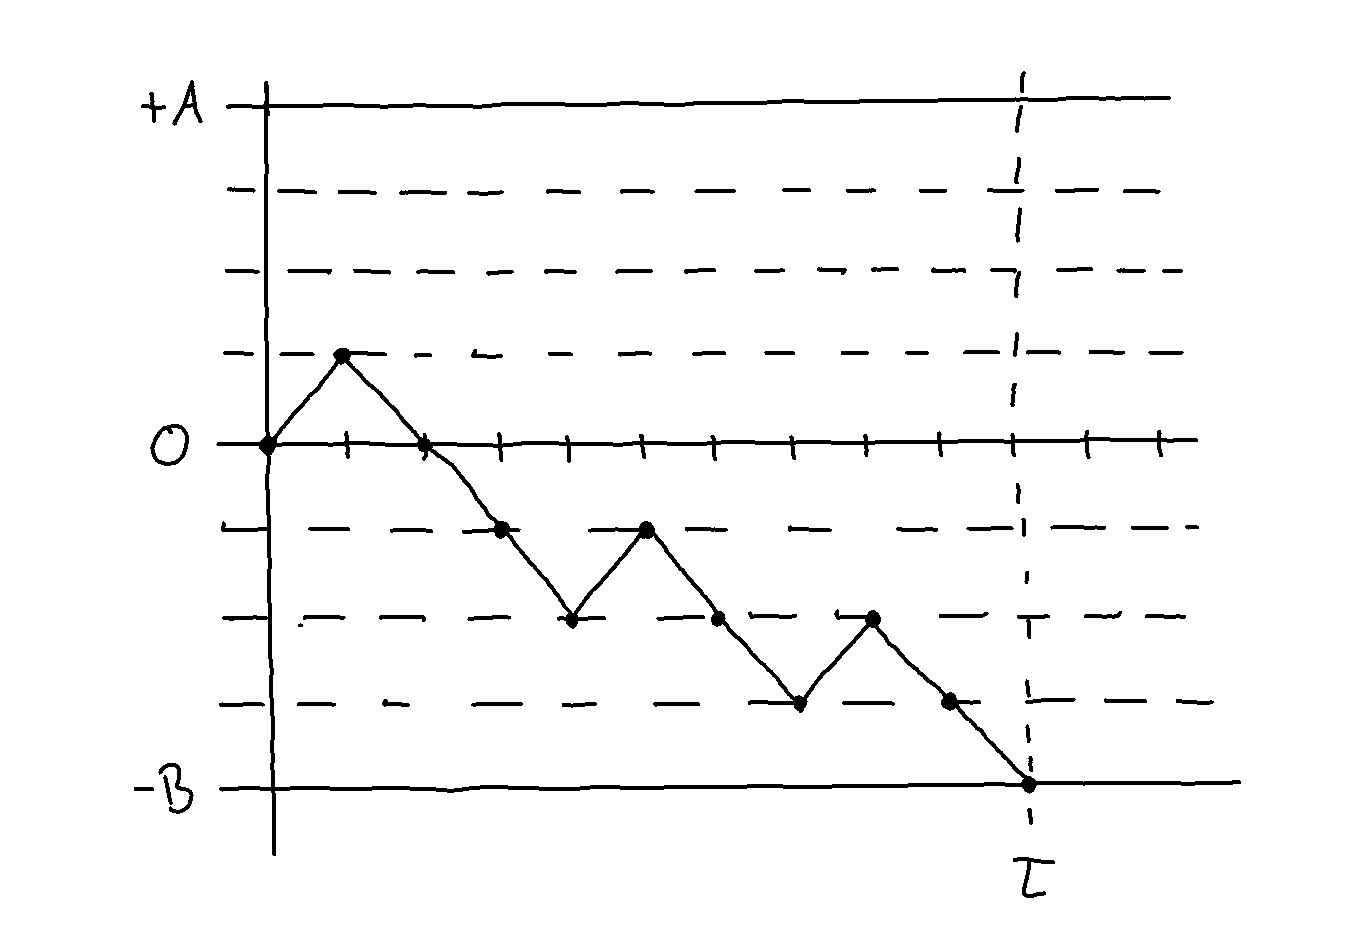
\includegraphics[width=0.75\textwidth]{pics/Sketch0.png}
			\caption{Beispiel für finite-Elemente-Funktionen in 1D}
			\label{AbbFiniteFunktionen}
		\end{center}
	\end{figure}
\end{definition}

\begin{bemerkung}\
	\begin{itemize}
		\item Für $m=k-1$ erhält man Splines.
		\item $\begin{aligned}
			S_h^{k,m}\subseteq H^{m+1}(\Omega)
		\end{aligned}$ wegen Satz \ref{satz1.4}
		\item $\begin{aligned}
			S_h^{0,m}
		\end{aligned}$ sind konstante Funktionen auf $(0,1)$ für $m\geq0$
		\item Die Räume haben folgende Dimensionen:
		\begin{align*}
			\dim\left(S_h^{k,-1}\right)&=(n+1)\cdot(k+1)\\
			\dim\left(S_h^{k,m}\right)&=\dim\left(S_h^{k,-1}\right)-n\cdot(m+1)\\
			\dim\left(S_{h,0}^{k,m}\right)&=\dim\left(S_h^{k,m}\right)-2
		\end{align*}
		Konkrete wichtige Beispiele:
		\begin{align*}
			\dim\left(S_h^{k,0}\right)&=(n+1)\cdot(k+1)-n\\
			\dim\left(S_{h,0}^{k,0}\right)&=(n+1)\cdot(k+1)-n-2=(n+1)\cdot(k-1)+n\\
			\dim\left(S_{h,0}^{1,0}\right)&=(n+1)\cdot 2-n-2=n\\
			\dim\left(S_{h,0}^{2,0}\right)&=(n+1)\cdot 3-n-2=2\cdot n+1
		\end{align*}
	\end{itemize}
\end{bemerkung}

Sei $\lbrace\varphi_j\rbrace_{j\in J}$ eine Basis von $S_h^{k,0}$
und Lösung $u_h\in S_{h,0}^{k,0}: u_h=\sum\limits_j u_j\cdot\varphi_j$\\
Diskretes Problem: Finde $u_h\in S_{h,0}^{k,0}$ so, dass
\begin{align*}
	&a(u_h,\varphi_h)=l(\varphi_h)&\qquad&\forall \varphi_h\in S_{h,0}^{k,0}\\
	\Longleftrightarrow &a(u_h,\varphi_i)=l(\varphi_i)&\qquad&\forall i
\end{align*}
In Matrix-Notation ergibt dies Folgendes:
\begin{align*}
	&A=(a_{i,j}),&&a_{i,j}:=a(\varphi_j,\varphi_i)\\
	&b=(b_i),&&b_i:=l(\varphi_i\nl
	&\qquad\Longleftrightarrow A\cdot U=b,\qquad U=(u_i)
\end{align*}
Hierbei heißt $A$ \textbf{Stiffness-Matrix}.

\begin{align*}
	S^{1,0}_{h,0}&=\text{span}\big\lbrace\varphi_i:1\leq i\leq n\big\rbrace,\qquad
	\varphi_i(t)=\left\lbrace\begin{array}{cl}
		\frac{t-t_{i-1}}{h_{i-1}}, &\falls t\in I_{i-1}\\
		\frac{t_{i+1}-t}{h_i}, &\falls t\in I_i\\
		0, &\sonst
	\end{array}\right.\\
	\big(\text{supp}(\varphi_i) &= [t_{i-1}, t_{i+1}]\big)\\
	\implies a_{i,j}&=0\text{ für }|i-j|>1\implies A\text{ ist Tridiagonalmatrix}
\end{align*}

\begin{figure}[!ht]
	\begin{center}
		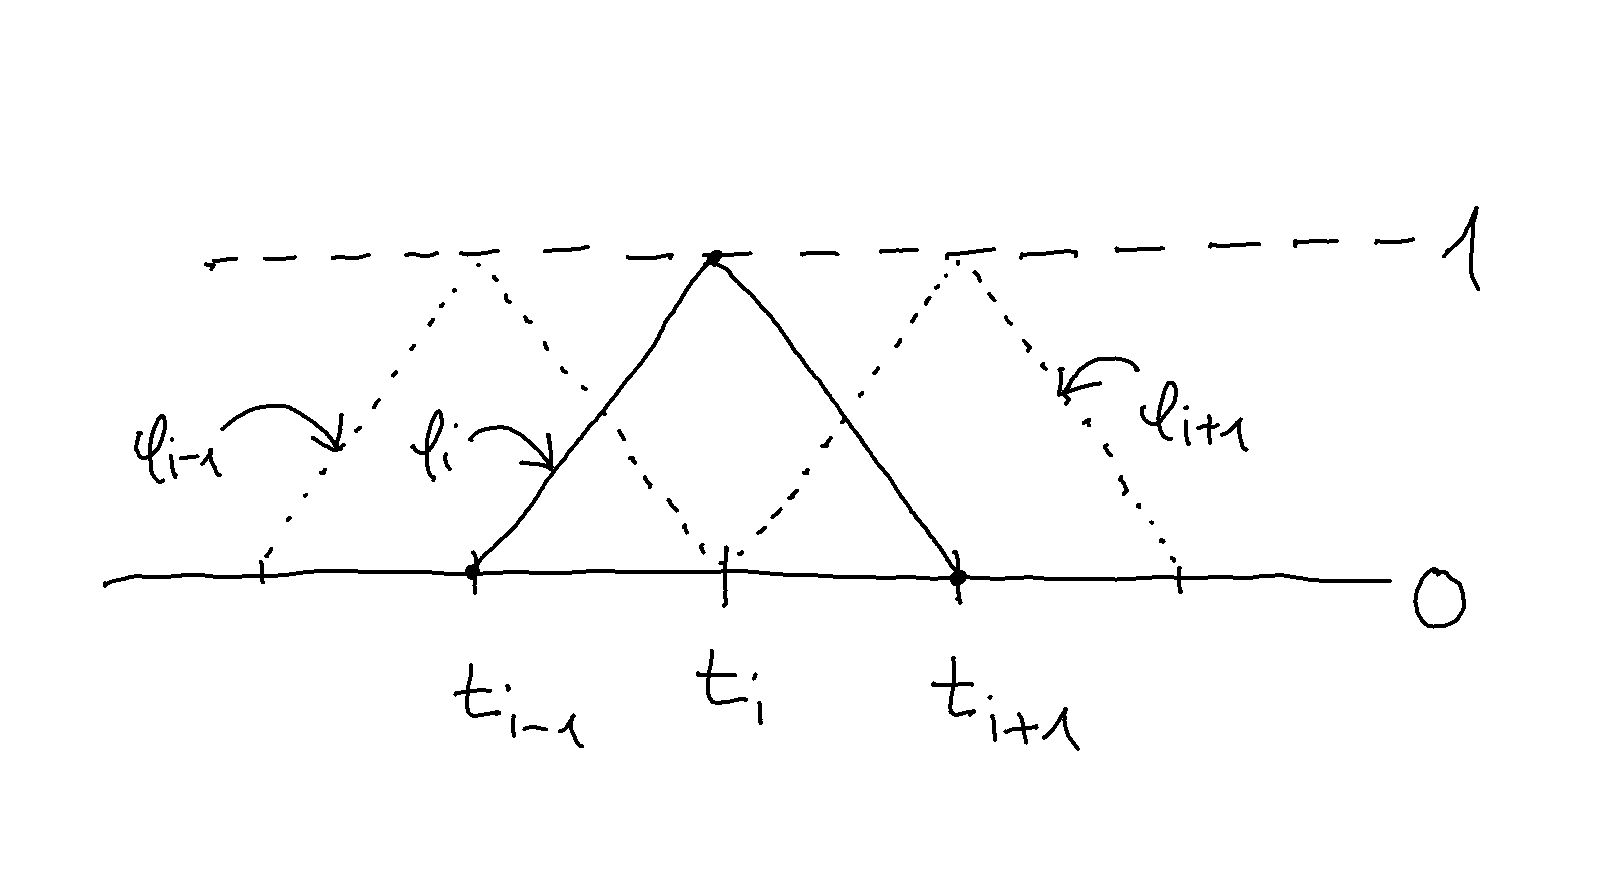
\includegraphics[width=0.75\textwidth]{pics/Sketch1.png}
		\caption{Hut-Funktionen}
		\label{AbbHutFunktionen}
	\end{center}
\end{figure}

\begin{figure}[!ht]
	\begin{center}
		\centering
\begin{tikzpicture}[scale=1]

% Achsen
\draw (0,0) -- ++(0,1.2);
\draw (0,0) -- ++(4,0);

% Funktion
\draw[red] (0,0) -- ++(2.5,0) -- ++(0.5,1) -- ++(0.5,-1) -- ++(0.5,0);
	
% Anstrich Y-Achse 
\draw (-0.1,1) -- ++(0.2,0);
	
% Anstriche X-Achse
\draw (0.5,-0.1) -- ++(0,0.2);
\draw (1  ,-0.1) -- ++(0,0.2);
\draw (1.5,-0.1) -- ++(0,0.2);
\draw (2  ,-0.1) -- ++(0,0.2);
\draw (2.5,-0.1) -- ++(0,0.2);
\draw (3  ,-0.1) -- ++(0,0.2);
\draw (3.5,-0.1) -- ++(0,0.2);
	
	
\filldraw[red] (0.5,0) circle (1.5pt);
\filldraw[red] (1  ,0) circle (1.5pt);
\filldraw[red] (1.5,0) circle (1.5pt);
\filldraw[red] (2  ,0) circle (1.5pt);
\filldraw[red] (2.5,0) circle (1.5pt);
\filldraw[red] (3  ,1) circle (1.5pt);
\filldraw[red] (3.5,0) circle (1.5pt);
	
	
\node at (-0.3,1) {1};
\node at (3.5,1) {$\varphi_j$};
\end{tikzpicture}

		\caption{einzelne Hut-Funktion}
		\label{AbbPhiHat}
	\end{center}
\end{figure}

\begin{align*}
	S_{h,0}^{2,0}&=\spann\big\lbrace\varphi_1,\ldots,\varphi_n,\psi_0,\ldots,\psi_n\big\rbrace,\qquad
	\psi_i(t)=\left\lbrace\begin{array}{cl}
		4\cdot\frac{(t-t_i)\cdot(t_{i+1}-t)}{h_i^2}, &\falls t\in I_i\\
		0 &\sonst
	\end{array}\right.
\end{align*}

\begin{figure}[!ht]
	\begin{center}
		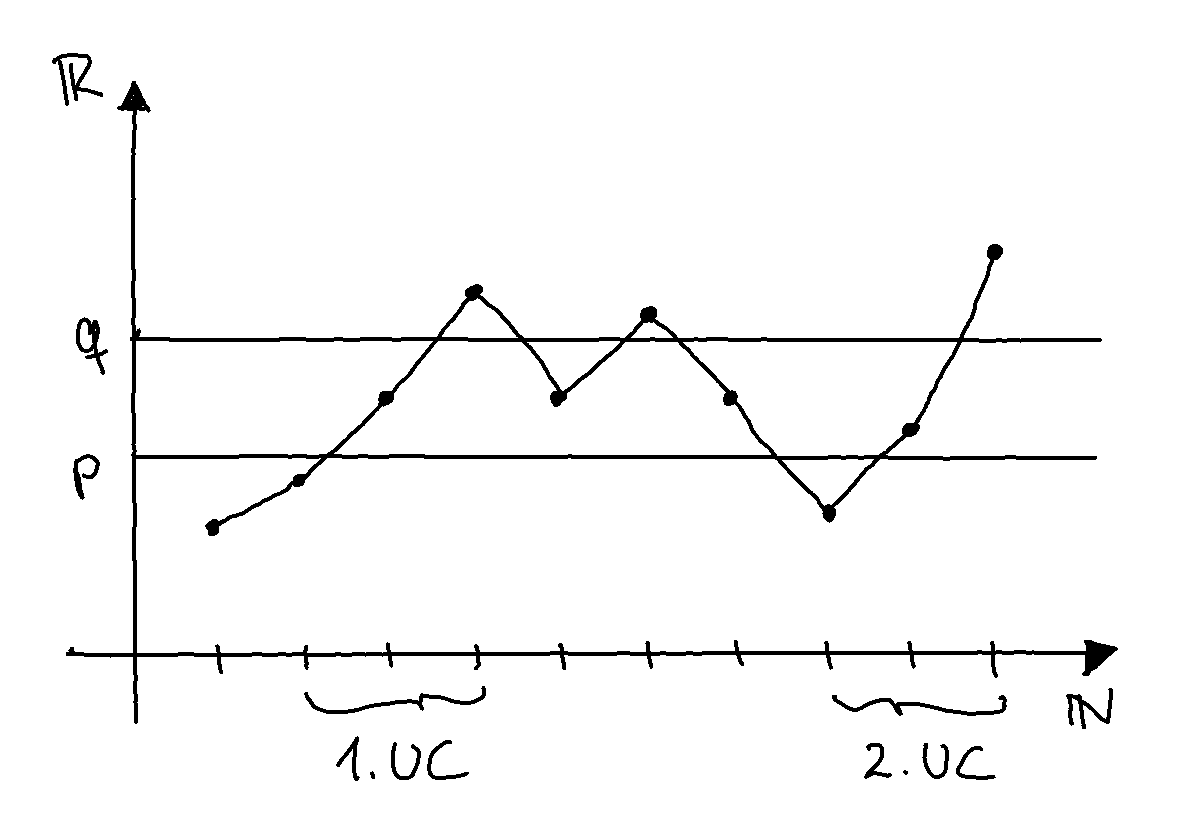
\includegraphics[width=0.5\textwidth]{./pics/Sketch2.png}
		\caption{einzelne zweifach diffbare finite-Elemente-Funktion}
		\label{AbbFiniteElementeFunktionZweifachDiffbar}
	\end{center}
\end{figure}

Die Stiffness-Matrix $A$ lässt sich als Blockmatrix schreiben:
\begin{align*}
	A=\begin{pmatrix}
		A_{LL} & A_{LQ}\\
		A_{QL} & A_{QQ}
	\end{pmatrix}
\end{align*}
wobei $A_{QQ}$ eine Diagonalmatrix ist. Somit:
\begin{align*}
	\begin{pmatrix}
		A_{LL} & A_{LQ}\\
		A_{QL} & A_{QQ}
	\end{pmatrix}\cdot\begin{pmatrix}
		U_L\\ U_Q
	\end{pmatrix}=
	\begin{pmatrix}
		b_L\\ b_Q
	\end{pmatrix}
\end{align*}
Dieses System von Gleichungen ist äquivalent zu:
\begin{align*}
	\big(A_{LL}-A_{LQ}\cdot A^{-1}_{QQ}\cdot A_{QL}\big)\cdot U_L&= b_L-A_{LQ}\cdot A^{-1}_{QQ}\cdot b_Q\\
	A_{QQ}\cdot U_Q&= b_Q-A_{QL}\cdot U_L
\end{align*}

\begin{theorem}[Approximationseigenschaft von 1D finiten Elementen]\label{theorem4.2}\enter
	Sei $u\in H^{k+1}(\Omega)\cap H^{1}_0(\Omega)$ für ein $k\geq1$. Dann gilt:
	\begin{align*}
		\inf\limits_{v_h\in S_{h,0}^{k,0}}\big|u-v_h\big|_{1,2}\leq h^k\cdot|u|_{k+1,2}
	\end{align*}
	(Hierbei ist $h$ wie oben der Maximalabstand.)
\end{theorem}

\begin{proof}
	Definiere Intervallweise die Funktion auf $I_i$ durch
	\begin{align*}
		v_h^\ast(t):=L_i(t)\qquad\forall t\in I_i,~\forall i\in\lbrace1,\ldots,n\rbrace
	\end{align*}
	wobei die $L_i$ die Lagrange-Interpolationen in $P_k$ bzgl. $t_i+\frac{s}{h}\cdot h_i,~0\leq j\leq h$ sind.\\
	Offenbar gilt $v_h^\ast\in S^{k,0}_{h,0}$. \\
	$u-v_n^\ast$ in $\overline{I_i}=[t_i,t_{i+1}]$ hat $(k+1)$ Nullen wegen der Interpolation. Somit hat $\big(u-v_h^\ast)^{(\mu)}$ $(k+1-\mu)$ Nullen.
	\begin{align*}
		\big|u-v_h^\ast\big|_{\mu,2,I_i}
		&=\left\Vert \big(u-v_h^\ast\big)^{(\mu)}\right\Vert_{0,2,I_i}\\
		&\stackrel{}{\leq}
		h_i\cdot\left|\big(u-v_h^\ast\big)^{(\mu)}\right|_{1,2,I_i}\\
		&=h_i\cdot\left|\big(u-v_h^\ast\big)^{(\mu+1)}\right|_{0,2,I_i}\\
		&\leq h_i\cdot\left|u-v_h^\ast\right|_{\mu+1,2,I_i}\\
		\implies
		\big|u-v_h^\ast\big|_{1,2,I_i}
		&\leq h_i^k\cdot\big|u-v_h^\ast\big|_{k+1,2,I_i} \\
		\overset{v_h^\ast|_{I_i}\in P_k}&=
		h_i^k\cdot |u|_{k+1,2,I_i}
	\end{align*}
	Somit folgt
	\begin{align*}
		\big| u-v_h^\ast\big|_{1,2,\Omega}
		&=\left(\sum\limits_{i=1}^n\big|u-v_h^\ast\big|^2_{1,2,I_i}\right)^{\frac{1}{2}}\\
		&\leq\left(\sum\limits_{i=1}^n \underbrace{h_i^{2\cdot k}}_{\leq h^{2\cdot k}} \big|u\big|^2_{k+1,2,I_i}\right)^{\frac{1}{2}}\\
		&\leq h^k\cdot |u|_{k+1,2,\Omega}
	\end{align*}
\end{proof}

\begin{lemma}\label{lemma4.3}
	Sei $u\in H^1((a,b))$ mit der Eigenschaft
	\begin{align*}
		\exists t^\ast\in[a,b]:u(t^\ast)=0.
	\end{align*}
	Dann gilt:
	\begin{align*}
		\Vert  u\Vert_{L^\infty}:=\max\limits_{t\in [a,b]}\big|u(t)\big|&\leq(b-a)^{\frac{1}{2}}\cdot |u|_{1,2}\\
		\Vert u\Vert_{0,2}&\leq(b-a)\cdot|u|_{1,2}
	\end{align*}
	Für alle $u\in H^1_0((a,b))$ gilt:
	\begin{align*}
		\left(1+(b-a)^2\right)^{\frac{1}{2}}\cdot\Vert u\Vert_{1,2}\leq|u|_{1,2}\leq\Vert u\Vert_{1,2}
	\end{align*}
\end{lemma}

\subsection*{Sturm-Liouville Problem}
\begin{align}\label{eqSturmLiouvillePDE}\tag{SturmLiouville}
	\left\lbrace\begin{array}{rll}
		-\big(p(x)\cdot u'(x)\big)'+q(x)\cdot u(x) &= f(x) &\text{ in } (0,1)\\
		u(0)=u(1)&=0 &
	\end{array}
	\right.
\end{align}
wobei
\begin{align*}
	&f\in L^2((0,1)),\\
	&q\in C\big([0,1]\big), &&q(x)\geq0\quad\forall x\in[0,1], \\
	&p\in C\big([0,1]\big), &&p(x)\geq p_0>0\quad\forall x\in [0,1]
\end{align*}
\begin{align*}
	a(v,w)=\int\limits_0^1 p(x)\cdot v'(x)\cdot w'(x)+q(x)\cdot v(x)\cdot w(x)\d x
\end{align*}

\begin{theorem}\label{theorem4.4}
	Sei $u\in H^1_0\big((0,1)\big)$ die eindeutige schwache Lösung von \eqref{eqSturmLiouvillePDE} und $u_h$ die zugehörige Lösung in $S_{h,0}^{k,0}$.
	Falls $u\in H^{k+1}\big((0,1)\big)$, dann gilt:
	\begin{align*}
		|u-u_h|_{1,2}&\leq c_1\cdot h^k\cdot |u|_{k+1,2}\\
		\Vert u-u_h\Vert_{0,2}&\leq c_1\cdot h^k\cdot |u|_{k+1,2}\\
		\mit c_1&=\frac{2}{p_0}\cdot\max\limits\big\lbrace \Vert p\Vert_{C^0},\Vert q\Vert_{C^0}\big\rbrace
	\end{align*}
	Falls zusätzlich die schwache Formulierung für alle $\varphi\in L^2\big((0,1)\big)$ eine eindeutige schwache Lösung
	\begin{align*}
		u_\varphi\in H^2\big((0,1)\big)\cap H^1_0\big((0,1)\big)\mit |u_\varphi|_{2,2}\leq c_2\cdot\Vert \varphi\Vert_{0,2}
	\end{align*}
	liefert, dann gilt
	\begin{align*}
		\big\Vert u-u_h\big\Vert_{0,2}\leq c_3\cdot h^{k+1}\cdot |u|_{k+1,2}
		\mit c_3=\frac{4\cdot c_2}{p_0}\cdot\max\limits\left\lbrace\Vert p\Vert^2_{C^0},\Vert q\Vert^2_{C^0}\right\rbrace
	\end{align*}
\end{theorem}

\subsection{FEM in 2D}

Nun der zweidimensionale Fall: Sei $\Omega\subseteq\R^2$ ein beschränktes Polygon. 
Nun zerlegen wir das Polygon in Dreiecke. 
Dieses Verfahren heißt \textbf{Dekomposition / Triangulation.} 
Dadurch erhalten wir eine Menge von \underline{offenen} (nach Konvention) Dreiecken $\lbrace K_i\rbrace_{i\in\lbrace1,\ldots,N\rbrace}$ mit den Eigenschaften:

\begin{enumerate}[label=(\roman*)]
	\item $\begin{aligned}
		\overline{\Omega}=\bigcup\limits_{i=1}^N \overline{K_i}
		\end{aligned}$
	\item $\begin{aligned}
		i\neq j\implies K_i\cap K_j=\emptyset
	\end{aligned}$
	\item Zulässigkeit: $\overline{K_i}\cap\overline{K_j}$ für $i\neq j$ ist
	\begin{itemize}
		\item leer oder
		\item ein einziger Punkt oder
		\item eine \ul{gemeinsame} Kante.
	\end{itemize}

	\begin{figure}[!ht]
		\begin{center}
			\begin{tikzpicture}[scale=1]

     
	
    % fill triangles
    \fill[red!40!white]   (0,0) -- ++(1,-0.5) -- ++(0.25,0.5) --cycle;
    \fill[blue!40!white]  (0,0) -- ++(1.25,0) --++(-0.75,0.25) --cycle;
    \fill[green!20!white]   (1.25,0) --++(-0.75,0.25) --++(1.75,0.25) --cycle;
    \fill[yellow!20!white]   (0.5,0.25) --++(1.75,0.25) --  ++(-2.75,0.5) --cycle;
	 
	% outline
	\draw (0,0) -- ++(1,-0.5) -- ++(0.25,0.5)-- ++(1,0.5) -- ++(-2.75,0.5)-- ++(1,-0.75)--cycle;

	% this is unrobust
	\draw (0,0) -- ++(1.25,0) --++(-0.75,0.25) --++(1.75,0.25);

\end{tikzpicture}
			\caption{beispielhafte Triangulation, $K_i$ disjunkt}
			\label{AbbTriangulierung}
		\end{center}
	\end{figure}

	\begin{figure}[!ht]
		\begin{center}
			\begin{tikzpicture}[scale=1]

	% outline
	\draw (0,0) -- ++(1.5,-1) -- ++(1.5,1)-- ++(-1.5,1) -- cycle;
	\draw (1.5,-1) -- ++(0,2);
	\draw (1.5,0) -- ++(1.5,0);
	
	% red cross
	\draw[thick,red] (0,-1) --++ (3,2);

	% dot middle
	\filldraw (1.5,0) circle (1.6pt);

\end{tikzpicture}
			\caption{Unzulässige Triangulation}
			\label{AbbUnzulaessigeTriangulierung}
		\end{center}
	\end{figure}
\end{enumerate}

Die Triangulation $\T$ ist formal definiert als Menge der Teildreiecke, also
\begin{align*}
	\T:=\lbrace K_1,\ldots,K_N\rbrace.
\end{align*} 

\subsection*{Raum der stetigen stückweise linearen Funktionen}
\begin{align*}
	V_h&:=\left\lbrace
	\begin{array}{rl}
		v\in C(\overline{\Omega}) : &v|_{K_i}\in P_1(K_i)~\forall i=1,\ldots,N,\\
		&v|_{\partial\Omega}=0
	\end{array}\right\rbrace
	\subseteq H^1_0(\Omega)\\
	P_1(K_i)&=\spann(\lbrace1,x,y\rbrace)\text{ (zwei-Dimensional, deshalb }x,y)\\
	P_2(K_i)&=\spann\big(\big\lbrace x^\alpha, |\alpha|\leq k\big\rbrace\big)\mit K\subseteq\R^d,~ x^{\alpha}:=x_1^{\alpha_1},\ldots,x_d^{\alpha_d}\\
	Q_k(K_i)&=\spann\big(\big\lbrace x^\alpha,\max\limits_i |\alpha_i|\leq k\big\rbrace\big)\\
	Q_1(K_i)&=\spann(\lbrace 1,x,y,xy\rbrace)\\
	\dim(V_h)&=\text{ Anzahl der inneren Knoten von der zulässigen Triangulierung}\\
\end{align*}

\begin{definition}[Finites Element]\enter %4.5
	Ein \textbf{finites Element} ist ein Tripel $(K,V,\Sigma)$ mit:
	\begin{enumerate}[label=(\roman*)]
		\item $K\subseteq\R^d$ ist nichtleer, offen, beschränkt und Lipschitz-berandet.
		\item $V=\big\lbrace f:K\to\R\big\rbrace$ ist endlich-dimensionaler Funktionenraum mit $m:=\dim(V)<\infty$. Sei $B_V:=\lbrace\varphi_1,\ldots,\varphi_m\rbrace$ eine Basis von $V$.
		Die Funktionen $v_i\in V$ heißen \textbf{lokale Basis / Shape-Funktionen / Form-Funktionen} genannt.
		\item Sei $\Sigma:=\lbrace N_1,\ldots,N_m\rbrace$ die eindeutige duale Basis zu $B_V$, d.h. es gilt (aus LAAG bekannt):
		\begin{align*}
			\forall i\in\lbrace 1,\ldots,m\rbrace:\exists! N_i\colon V\to\R:\forall j\in\lbrace1,\ldots,m\rbrace: N_i(\varphi_j)=\delta_{i,j}
		\end{align*}				
		Somit ist $\Sigma$ eine Basis von $V^\ast$ bestehend aus $m$ linearen Funktionalen $N_i$, den sogenannten \textbf{Nodal-Funktionalen / Freiheitsgrade / DOFs.}
	\end{enumerate}
\end{definition}

\begin{bemerkung} % war in VL anders
	Die Nodal-Funktional-Menge $\Sigma$ gilt: 
		\begin{align*}
			\Sigma\text{ ist Basis von }V^\ast\Longleftrightarrow\Sigma\text{ ist \textbf{$V$-unisolvent}, d. h.:}\\
			\forall (\alpha_1,\ldots,\alpha_m)\in\R^m:\exists! v\in V:\forall i\in\lbrace1,\ldots,m\rbrace:N_i(v)=\alpha_i
		\end{align*}
\end{bemerkung}

\begin{proof}
	\underline{Zeige Basis $\implies V$-unisolvenz:}\\
	Sei $i\in\lbrace1,\ldots,m\rbrace$ und $\alpha_i\in\R$ beliebig.\nl
	\underline{Existenz}:
	Da $B_V$ eine Basis von $V$ ist, gilt 
	\begin{align*}
		\forall v\in V:\exists v_1,\ldots,v_m\in\R:v=\sum\limits_{j=1}^m\varphi_j\cdot v_j
	\end{align*}
	und somit
	\begin{align*}
		N_i(v)
		=N_i\left(\sum\limits_{j=1}^m\varphi_j\cdot v_j\right)
		\overset{\text{Lin}}=
		\sum\limits_{j=1}^m v_j\cdot \underbrace{N_i(\varphi_j)}_{=\delta_{i,j}}=v_i\qquad\forall v\in V.
	\end{align*}
	Wähle als $v_i:=\alpha_i\in\R$.\nl
	\underline{Eindeutigkeit:}
	Seien $v,\tilde{v}\in V$ mit $N_i(v)=\alpha_i=N_i(\tilde{v})$.
	Dann gilt schon $v=\tilde{v}$, denn:
	\begin{align*}
		v_i=N_i(v)=\alpha_i=N_i(\tilde{v})=\tilde{v_i}\qquad\forall i\in\lbrace1,\ldots,m\rbrace	
	\end{align*}	
	\underline{Zeige $V$-unisolvenz $\implies$ Basis}:
	Nachrechnen. 
\end{proof}

Es ist sinnvoll und naheliegend für ein Finites-Element $(K,V,\Sigma)$ $\dim(V)=|\Sigma|=n$ zu wählen, mit $n$ Anzahl der Ecken des Polygons $K\subseteq\R^2$.
Nodal-Funktionale bilden Funktionen auf deren Werte an den "Ecken" ab.

\begin{definition}[affin äquivalente finite Elemente]\enter %4.6
	Zwei finite Elemente $(K,V,\Sigma)$ und $(\hat{K},\hat{V},\hat{\Sigma})$ heißen \textbf{affin äquivalent}
	\begin{align*}
		:\Longleftrightarrow\exists F:\R^d\to\R^d\text{ affin \& invertierbar v.d.F. }
		\hat{x}\mapsto B_k\cdot\hat{x}+b_k\mit B_k\in\R^{d\times d},b_k\in\R^d
	\end{align*}
	mit den Eigenschaften
	\begin{enumerate}[label=(\arabic*)]
		\item $\begin{aligned}
			K=F(\hat{K})
		\end{aligned}$
		\item $\begin{aligned}
			V=\Big\lbrace v: K\to\R~\Big|~\exists\hat{v}\in\hat{V}: v=\hat{v}\circ F^{-1}\Big\rbrace
		\end{aligned}$
		\item $\begin{aligned}
			\Sigma=\Big\lbrace N:V\to\R~\Big|~\exists\hat{N}\in\hat{\Sigma}: N(v)=\hat{N}(v\circ F)\Big\rbrace
		\end{aligned}$
	\end{enumerate}
\end{definition}

\begin{beisp}\
	\begin{figure}[H]
		\begin{center}
			\centering
\begin{tikzpicture}[scale=2]


\draw[thick] (0,0) -- ++(0,1) -- ++(1,-1)--cycle;
\filldraw (0,0)         circle (0.8pt);
\filldraw (0,0) ++(1,0) circle (0.8pt);
\filldraw (0,0) ++(0,1) circle (0.8pt);
\fill[black,font=\footnotesize] (0,0) node[below] {1 $(0,0)$}
								(0,0) ++(1,0) node[below] {2 $(1,0)$}
								(0,0) ++(0,1) node[above] {3 $(0,1)$};
								
\draw[thick] (2.2,0) -- ++(2,0) -- ++(-1,1)--cycle;
\filldraw (2.2,0)         circle (0.8pt);
\filldraw (2.2,0) ++(2,0) circle (0.8pt);
\filldraw (2.2,0) ++(1,1) circle (0.8pt);
\fill[black,font=\footnotesize] (2.2,0) node[below] {1 $(a_1,a_2)$}
								(2.2,0) ++(2,0) node[below] {2 $(b_1,b_2)$}
								(2.2,0) ++(1,1) node[above] {3 $(c_1,c_2)$};								
								
												
\node at (1.5,1) {$F$};				
\draw[thick,-to] (1.2,0.5) .. controls (1.4,0.8) and (1.9,0.9) .. (2.2, 0.8);
\draw[thick] (0,0) -- ++(0,1) -- ++(1,-1)--cycle;

\end{tikzpicture}

			\caption{affin äquivalente Triangulation}
			\label{AbbAffinEquivTriang}
		\end{center}
	\end{figure}

	\begin{align*}
		F:\left\lbrace\begin{array}{l}
			(0,0)\mapsto(a_1,a_2)\\
			(1,0)\mapsto(b_1,b_2)\\
			(0,1)\mapsto(c_1,c_2)
		\end{array}\right.
		\qquad\qquad
		\begin{matrix}
			\hat{N}_1(\hat{v})&=\hat{v}(0,0) &&N_1(v)=v(a_1,a_2)\\
			\hat{N}_2(\hat{v})&=\hat{v}(1,0) &&N_2(v)=v(b_1,b_2)\\
			\hat{N}_3(\hat{v})&=\hat{v}(0,1) &&N_3(v)=v(c_1,c_2)
		\end{matrix}
	\end{align*}
\end{beisp}

Sei $V$ ein Vektorraum mit Basis $\lbrace\varphi_1,\ldots,\varphi_m\rbrace$. Setze
\begin{align*}
	\Sigma&=\lbrace N_1,\ldots,N_m\rbrace\\
	M&=(m_{i,j}),\qquad m_{i,j}:=N_i(\varphi_j)\\
	M&\text{ invertierbar }\Longleftrightarrow \text{ unisolvent}
\end{align*}
Unisolvenz: Gegeben $\alpha_1,\ldots,\alpha_m\in\R$. Gibt es ein eindeutiges $v\in V$
\begin{align*}
	N_i(v)&=\alpha_i,\qquad i\in\lbrace1,\ldots,m\rbrace\\
	\stackrel{v=\sum\limits_{j=1}^m c_j\cdot\varphi_j}{\Longleftrightarrow}\quad
	\sum\limits_{j=1}^m N_i(\varphi_j)\cdot c_j&=\alpha_i\\
	\Longleftrightarrow
	M\cdot c&=\alpha
\end{align*}

\begin{beispiel} % war nicht in VL
	Dreiecke:
	\begin{itemize}
		\item $P_0$: stückweise konstante FEM,\\ $\dim(P_0(K))=1$
		\item $P_1$: konformes stückweises linearen FEM, $\dim(P_1(K))=d+1\overset{d=2}{=}3$
		\item $P_2$: konforme stückweise quadratische FEM, $\dim(P_2(K))=\frac{(d+1)\cdot(d+2)}{2}=\overset{d=2}{=}6$
		\item $P_3$: konforme stückweise kubische FEM, $\dim(P_3(K))=\frac{(d+1)\cdot(d+2)\cdot(d+3)}{6}\overset{d=2}{=}10$
	\end{itemize}
	
	\begin{figure}[H] % oder ht!
		\begin{center}
			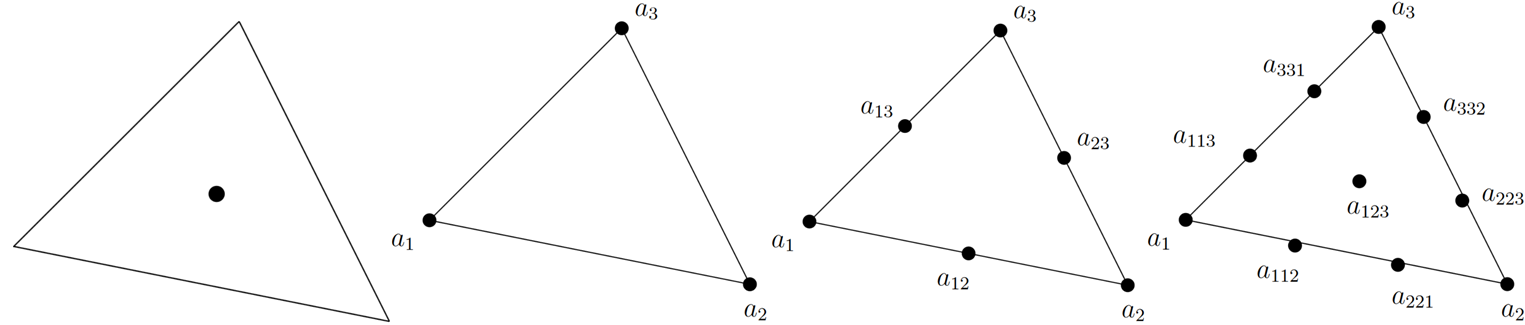
\includegraphics[width=1\textwidth]{./pics/FEM_Dreieck.png}
			\caption{Nodal Functionals für $P_0,P_1,P_2,P_3$}
			\label{AbbFEM-Dreieck}
		\end{center}
	\end{figure}

	Quadrate:
	\begin{itemize}
		\item $Q_0$: stückweise konstantes FEM: $\dim(Q_0(K))=1$
		\item $Q_1$: konforme stückweise $d$-lineare FEM, $\dim(Q_1(K))=2^d\overset{d=2}{=}4$
		\item $Q_2$: konforme stückweise $d$-dimensionalen FEM, $\dim(Q_2(K))=3^d\overset{d=2}{=}8$
		\item $Q_3$: konforme stückweise $d$-kubische FEM, $\dim(Q_3(K))=4^d\overset{d=2}{=}16$.
	\end{itemize}
	
	\begin{figure}[H] % oder ht!
		\begin{center}
			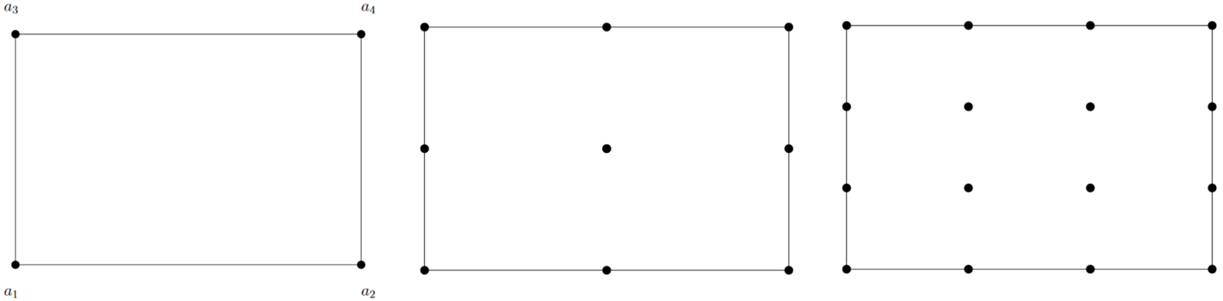
\includegraphics[width=1\textwidth]{./pics/FEM_Quadrat.png}
			\caption{Nodal Functionals für $Q_1,Q_2,Q_3$}
			\label{AbbFEM-Qudrat}
		\end{center}
	\end{figure}
\end{beispiel}

\begin{definition}[globales Nodal-Funktional / globale Freiheitsgrade (dof)]\enter
	Seien $(K,V,\Sigma)$ und $(K',V',\Sigma')$ Finite-Elemente.
	Zwei lokale Nodal-Funktionale $N_i^K\in\Sigma$ und $N_j^{K'}\in\Sigma'$ \textbf{gehören zum selben globalen Freiheitsgrad}, i.Z.
	\begin{align*}
		N_i^K\sim N_j^{K'}:\Longleftrightarrow N_i^K(\varphi|_K)=N_j^{K'}(\varphi|_{K'})\qquad\forall\varphi\in C^\infty(U)
	\end{align*}
	wobei $U\subseteq\Omega$ eine offene Menge mit der Eigenschaft $\overline{K\cup K'}\subseteq U$ ist.\\
	Anschaulich: Zwei Nodal-Funktionale sind $\sim$-äquivalent, wenn sie dieselbe Ecke beschreiben.
	$\sim$ ist eine Äquivalenzrelation.\\
	Die \textbf{Menge aller globalen Freiheitsgrade} einer Triangulation $\T=\lbrace K_1,\ldots,K_N\rbrace$ bezeichnen wir mit
	\begin{align*}
		\Sigma_h:=\left.\left(\bigcup\limits_{i=1}^N\bigcup\limits_{j=1}^m N_j^{K_i}\right)\right/\sim
	\end{align*}
	Für $[N]_\sim\in\Sigma_h$ bezeichne
	\begin{align*}
		\Lambda\big([N]_\sim\big):=\left\lbrace N\in[N]_\sim\right\rbrace
	\end{align*}		
	die Menge alle lokalen Freiheitsgrade $N$, die zu $[N]_\sim$ gehören.
\end{definition}

\begin{figure}[H] % oder ht!
	\begin{center}
		% This work is licensed under the Creative Commons
% Attribution-NonCommercial-ShareAlike 4.0 International License. To view a copy
% of this license, visit http://creativecommons.org/licenses/by-nc-sa/4.0/ or
% send a letter to Creative Commons, PO Box 1866, Mountain View, CA 94042, USA.
% vim: set noexpandtab:

% the following tikz picture was auto-generated by:
% https://www.mathcha.io/editor

\tikzset{every picture/.style={line width=0.75pt}} %set default line width to 0.75pt        

\begin{tikzpicture}[x=0.75pt,y=0.75pt,yscale=-1,xscale=1]
%uncomment if require: \path (0,300); %set diagram left start at 0, and has height of 300

%Shape: Rectangle [id:dp14549454055533384] 
\draw   (64,2.93) -- (345,2.93) -- (345,290.93) -- (64,290.93) -- cycle ;
%Straight Lines [id:da9627683453327494] 
\draw    (64,2.93) -- (345,290.93) ;


%Straight Lines [id:da9434997856090799] 
\draw    (345,2.93) -- (64,290.93) ;


%Straight Lines [id:da169571524037062] 
\draw    (100,130) ;


%Shape: Circle [id:dp7836721006446373] 
\draw   (186.18,146.69) .. controls (186.9,144.02) and (189.65,142.45) .. (192.31,143.18) .. controls (194.98,143.9) and (196.55,146.65) .. (195.82,149.31) .. controls (195.1,151.98) and (192.35,153.55) .. (189.69,152.82) .. controls (187.02,152.1) and (185.45,149.35) .. (186.18,146.69) -- cycle ;
%Shape: Circle [id:dp7887685534943322] 
\draw   (214.18,146.69) .. controls (214.9,144.02) and (217.65,142.45) .. (220.31,143.18) .. controls (222.98,143.9) and (224.55,146.65) .. (223.82,149.31) .. controls (223.1,151.98) and (220.35,153.55) .. (217.69,152.82) .. controls (215.02,152.1) and (213.45,149.35) .. (214.18,146.69) -- cycle ;
%Shape: Circle [id:dp792561043036806] 
\draw   (198.18,161.69) .. controls (198.9,159.02) and (201.65,157.45) .. (204.31,158.18) .. controls (206.98,158.9) and (208.55,161.65) .. (207.82,164.31) .. controls (207.1,166.98) and (204.35,168.55) .. (201.69,167.82) .. controls (199.02,167.1) and (197.45,164.35) .. (198.18,161.69) -- cycle ;
%Shape: Circle [id:dp5381851880499974] 
\draw   (200.18,131.69) .. controls (200.9,129.02) and (203.65,127.45) .. (206.31,128.18) .. controls (208.98,128.9) and (210.55,131.65) .. (209.82,134.31) .. controls (209.1,136.98) and (206.35,138.55) .. (203.69,137.82) .. controls (201.02,137.1) and (199.45,134.35) .. (200.18,131.69) -- cycle ;
%Shape: Circle [id:dp44002878595191575] 
\draw   (78.18,282.69) .. controls (78.9,280.02) and (81.65,278.45) .. (84.31,279.18) .. controls (86.98,279.9) and (88.55,282.65) .. (87.82,285.31) .. controls (87.1,287.98) and (84.35,289.55) .. (81.69,288.82) .. controls (79.02,288.1) and (77.45,285.35) .. (78.18,282.69) -- cycle ;
%Shape: Circle [id:dp42740284154555863] 
\draw   (67.18,267.69) .. controls (67.9,265.02) and (70.65,263.45) .. (73.31,264.18) .. controls (75.98,264.9) and (77.55,267.65) .. (76.82,270.31) .. controls (76.1,272.98) and (73.35,274.55) .. (70.69,273.82) .. controls (68.02,273.1) and (66.45,270.35) .. (67.18,267.69) -- cycle ;
%Shape: Circle [id:dp6205100758907591] 
\draw   (319.18,279.69) .. controls (319.9,277.02) and (322.65,275.45) .. (325.31,276.18) .. controls (327.98,276.9) and (329.55,279.65) .. (328.82,282.31) .. controls (328.1,284.98) and (325.35,286.55) .. (322.69,285.82) .. controls (320.02,285.1) and (318.45,282.35) .. (319.18,279.69) -- cycle ;
%Shape: Circle [id:dp12003747556472932] 
\draw   (331.18,265.69) .. controls (331.9,263.02) and (334.65,261.45) .. (337.31,262.18) .. controls (339.98,262.9) and (341.55,265.65) .. (340.82,268.31) .. controls (340.1,270.98) and (337.35,272.55) .. (334.69,271.82) .. controls (332.02,271.1) and (330.45,268.35) .. (331.18,265.69) -- cycle ;
%Shape: Circle [id:dp3476040811313178] 
\draw   (333.18,19.69) .. controls (333.9,17.02) and (336.65,15.45) .. (339.31,16.18) .. controls (341.98,16.9) and (343.55,19.65) .. (342.82,22.31) .. controls (342.1,24.98) and (339.35,26.55) .. (336.69,25.82) .. controls (334.02,25.1) and (332.45,22.35) .. (333.18,19.69) -- cycle ;
%Shape: Circle [id:dp21135819336466033] 
\draw   (323.18,9.69) .. controls (323.9,7.02) and (326.65,5.45) .. (329.31,6.18) .. controls (331.98,6.9) and (333.55,9.65) .. (332.82,12.31) .. controls (332.1,14.98) and (329.35,16.55) .. (326.69,15.82) .. controls (324.02,15.1) and (322.45,12.35) .. (323.18,9.69) -- cycle ;
%Shape: Circle [id:dp08585658948454522] 
\draw   (78.18,9.69) .. controls (78.9,7.02) and (81.65,5.45) .. (84.31,6.18) .. controls (86.98,6.9) and (88.55,9.65) .. (87.82,12.31) .. controls (87.1,14.98) and (84.35,16.55) .. (81.69,15.82) .. controls (79.02,15.1) and (77.45,12.35) .. (78.18,9.69) -- cycle ;
%Shape: Circle [id:dp07079948382140533] 
\draw   (65.18,21.69) .. controls (65.9,19.02) and (68.65,17.45) .. (71.31,18.18) .. controls (73.98,18.9) and (75.55,21.65) .. (74.82,24.31) .. controls (74.1,26.98) and (71.35,28.55) .. (68.69,27.82) .. controls (66.02,27.1) and (64.45,24.35) .. (65.18,21.69) -- cycle ;
%Shape: Circle [id:dp6214173079072771] 
\draw  [color={rgb, 255:red, 208; green, 2; blue, 27 }  ,draw opacity=1 ] (179.5,146.93) .. controls (179.5,133.13) and (190.69,121.93) .. (204.5,121.93) .. controls (218.31,121.93) and (229.5,133.13) .. (229.5,146.93) .. controls (229.5,160.74) and (218.31,171.93) .. (204.5,171.93) .. controls (190.69,171.93) and (179.5,160.74) .. (179.5,146.93) -- cycle ;
%Shape: Circle [id:dp8527921748422009] 
\draw  [color={rgb, 255:red, 208; green, 2; blue, 27 }  ,draw opacity=1 ] (314.69,274.39) .. controls (314.69,265.8) and (321.66,258.82) .. (330.26,258.82) .. controls (338.85,258.82) and (345.82,265.8) .. (345.82,274.39) .. controls (345.82,282.99) and (338.85,289.96) .. (330.26,289.96) .. controls (321.66,289.96) and (314.69,282.99) .. (314.69,274.39) -- cycle ;
%Shape: Circle [id:dp9683122242620462] 
\draw  [color={rgb, 255:red, 208; green, 2; blue, 27 }  ,draw opacity=1 ] (316.12,15.82) .. controls (316.12,7.23) and (323.09,0.26) .. (331.69,0.26) .. controls (340.29,0.26) and (347.26,7.23) .. (347.26,15.82) .. controls (347.26,24.42) and (340.29,31.39) .. (331.69,31.39) .. controls (323.09,31.39) and (316.12,24.42) .. (316.12,15.82) -- cycle ;
%Shape: Circle [id:dp7791705596437565] 
\draw  [color={rgb, 255:red, 208; green, 2; blue, 27 }  ,draw opacity=1 ] (61.74,17.18) .. controls (61.74,8.58) and (68.71,1.61) .. (77.31,1.61) .. controls (85.91,1.61) and (92.88,8.58) .. (92.88,17.18) .. controls (92.88,25.77) and (85.91,32.74) .. (77.31,32.74) .. controls (68.71,32.74) and (61.74,25.77) .. (61.74,17.18) -- cycle ;
%Shape: Circle [id:dp5325582065155569] 
\draw  [color={rgb, 255:red, 208; green, 2; blue, 27 }  ,draw opacity=1 ] (62.12,275.26) .. controls (62.12,266.66) and (69.09,259.69) .. (77.69,259.69) .. controls (86.29,259.69) and (93.26,266.66) .. (93.26,275.26) .. controls (93.26,283.85) and (86.29,290.82) .. (77.69,290.82) .. controls (69.09,290.82) and (62.12,283.85) .. (62.12,275.26) -- cycle ;

% Text Node
\draw (111,139) node  [align=left] {K1};
% Text Node
\draw (201,233) node  [align=left] {K2};
% Text Node
\draw (207,59) node  [align=left] {K3};
% Text Node
\draw (288,142) node  [align=left] {K4};


\end{tikzpicture}














		\caption{Hier werden die 12 DOFs der 4 FEMs per Äquivalenzrelation (rot) zu 5 globalen DOFs zusammengefasst.}
		\label{AbbGlobalDegreesOfFreedom}
	\end{center}
\end{figure}

\begin{definition}[Raum der finiten Elemente]\enter
	Sei $\T_h=\lbrace K_1,\ldots,K_N\rbrace$ eine Triangulation von $\Omega$ und seien\\ $\big((K_i,V_i(K_i),\Sigma_i(K_i)\big),i\in\lbrace1,\ldots,N\rbrace$ die zugehörigen Finite-Elemente.\\
	Ein \textbf{Finite-Elemente-Raum} $V_h$ ist gegeben durch
	\begin{align*}
		V_h:=\Bigg\lbrace v=(v_{K})_{K\in\T_h}\colon\bigcup\limits_{i=1}^N K_i\to\R\Bigg|
		\begin{array}{c}
			\forall [N]_\sim\in\Sigma_h:\forall N_i^{K},N_j^{K'}\in\Lambda([N]_\sim):\\
			N_i^{K}(v|_K)=N_j^{K'}(v|_{K'})
		\end{array}
		\Bigg\rbrace
	\end{align*}
	wobei $(K,V(K),\Sigma(K)),K\in\T_h$ finite Elemente sind.
	Im FEM-Raum liegen praktisch alle Funktionen $v:\Omega\to\R$ und es gibt eine Art globales Nodal-Funktional $N:(\Omega\to\R)\to\R$ (globales DOF), siehe Abbildung \ref{AbbGlobalDegreesOfFreedom}.
	Eine Funktion $v_h\in V_h$ ist eindeutig bestimmt durch die Werte des globalen DOFs $N(v_h)$.
\end{definition}

Familie aller affin äquivalenten Finiten-Elementen
\begin{align*}
	\big(K,V(K),\Sigma(K)\big)\sim\big(\hat{K},\hat{V},\hat{\Sigma}\big)
\end{align*}
Interpolation:
\begin{align*}
	I_h(v):=\sum\limits_{i=1}^n N_i(v)\cdot\varphi_i\in V_h
\end{align*}
wobei $\Sigma_h=\lbrace N_1,\ldots,N_n\rbrace\text{ und }\lbrace\varphi_1,\ldots,\varphi_n\rbrace$ eine Basis von $V_h$ ist mit der Eigenschaft $N_i(\varphi_j)=\delta_{i,j}$.\nl
\textbf{Wichtig:} Die Interpolationsfunktion erfüllt eine Lokalisierungseigenschaft:
\begin{align*}
	\big(I_h(v)\big)\big|_K&=I_h^K\big(v|_K\big)\quad\text{wobei}\\ I_h^K(v)&=\sum\limits_{i=1}^{m_K} N_i^{(K)}(v)\cdot\varphi_i^K,\qquad N_i^K(\varphi_j^K)=\delta_{i,j}\qquad\Sigma(K)=\left\lbrace N_1^K,\ldots,N_{m_K}^K\right\rbrace
\end{align*}

\begin{theorem}\label{theorem4.9}
	Seien $K,\hat{K}\subseteq\R^d$ zwei affin äquivalente offene  Teilmengen des $\R^d$, d. h. es existiert eine affine bijektive Abbildung
	\begin{align*}
		F:\hat{K}\to K,\qquad \hat{x}\mapsto B_K\cdot\hat{x}+ b_K\qquad\mit B_K\in\R^{d\times d}\text{ invertierbar und }b_K\in\R^d
	\end{align*}
	Falls $v\in W^{m,p}(K)$ für $m\geq0,p\in[1,\infty)$, dann gehört $\hat{v}:=v\circ F$ zu $W^{m,p}(\hat{K})$ und wir erhalten
	\begin{align*}
		\big|\hat{v}\big|_{m,p,\hat{K}}\leq c\cdot\Vert B_K\Vert^m\cdot\big|\det(B_K)\big|^{-\frac{1}{p}}\cdot|v|_{m,p,K}
	\end{align*}
	wobei $c=c(m,d)$ eine Konstante ist und $\Vert\cdot\Vert$ eine Matrixnorm, die durch die euklidische Vektornorm induziert wird.\\
	Zusätzlich gilt:
	\begin{align*}
		|v|_{m,p,K}&\leq c\cdot\Vert B_K^{-1}\Vert^m\cdot\big|\det(B_K)\big|^{\frac{1}{p}}\cdot|\hat{v}|_{m,p,\hat{K}}\\
		F^{-1}(x)&=B_K^{-1}\cdot x-B_K^{-1}\cdot b_K
	\end{align*}
\end{theorem}

\begin{lemma}\label{lemma4.10}
	Seien $K,\hat{K}$ affin äquivalent mit $F(\hat{x})=B_K\cdot\hat{x}+b_K$. Dann gilt:
	\begin{align*}
		\Vert B_K\Vert&\leq\frac{h_K}{\hat{\rho}},\qquad\Vert B_K^{-1}\Vert\leq\frac{\hat{h}}{\rho_K}\qquad\text{wobei}\\
		h_K&:=\diam(K):=\sup\limits_{x,y\in K}\Vert x-y\Vert\\
		\rho_K&:=\sup\big\lbrace\diam(S):S\subseteq K\text{ Sphäre}\big\rbrace
	\end{align*}
\end{lemma}

\begin{proof}
	\begin{align*}
		\Vert B_K\Vert&=\sup\limits_{z\neq0}\frac{\Vert B_K \cdot z\Vert}{\Vert z\Vert}=\frac{1}{\hat{\rho}}\cdot\sup\limits_{\Vert z\Vert=\hat{\rho}}\Vert B_K \cdot z\Vert
	\end{align*}
	Für alle $\eta$ mit $\Vert \eta\Vert=\hat{\rho}$ existieren zwei Punkte $\hat{x},\hat{y}\in\hat{K}$ so, dass $\eta=\hat{x}-\hat{y}$. Seien $x=F(\hat{x}),y=F(\hat{y})$. Dann gilt:
	\begin{align*}
		x-y&=B_K\cdot\hat{x}+b_K-\big(B_K\cdot\hat{y}+b_K\big)=B_K\cdot(\hat{x}-\hat{y})=B_K \cdot \eta\\
		\Vert B_K\cdot \eta\Vert&=\Vert x-y\Vert\leq h_K\\
		\implies \Vert h_K\Vert&\leq\frac{1}{\hat{\rho}}\cdot\sup\limits_{\Vert y\Vert=\hat{\rho}}\underbrace{\Vert B_K\cdot \eta\Vert}_{\leq h_K}\leq\frac{h_K}{\hat{\rho}}
	\end{align*}
\end{proof}

\begin{lemma}[Deny-Lions]\label{lemma4.11DenyLions}\enter
	Sei $P_r(K)$ der Raum aller Polynome mit höchstens Grad $r$. Dann gilt:
	\begin{align*}
		\exists c(K)>0:\inf\limits_{P\in P_r(K)}\Vert v\pm P\Vert_{r+1,p,K}\leq c(K)\cdot |v|_{r+1,p,K}\qquad\forall v\in W^{r+1,p}(K)
	\end{align*}
	(Hier $\pm$, da es egal ist, ob $-$ oder $+$, da $P\in P_r(K)\gdw -P\in P_r(K)$.)
\end{lemma}

\begin{proof}
	\begin{align*}
		n:=\dim \big(P_r(K)\big)=\begin{pmatrix}
			r+d\\ d
		\end{pmatrix}\text{ (Binomialkoeffizient)}
	\end{align*}
	Setze  für $\alpha\in\N_0^d\mit|\alpha|\leq r $:
	\begin{align*}
		N_\alpha:W^{r+1,p}(K)\to\R,\qquad v\mapsto\int\limits_K D^\alpha v\d x\\
		\alpha\longleftrightarrow x^\alpha =\prod\limits_{i=1}^d x_i^{\alpha_i}
	\end{align*}
	Also ist $\big\lbrace N_\alpha:|\alpha|\leq r\big\rbrace$ unisolvent auf $P_r(K)$.
	\begin{align*}
		\implies\left.
		\begin{array}{cl}
			N_\alpha(p)=0, &\forall |\alpha|\leq r \\
			p\in P_r(K)&
		\end{array}
		\right\rbrace
		\implies p\equiv 0
	\end{align*}
	Wir werden die Ungleichung
	\begin{align}\label{eqProof4.11Stern}\tag{$\ast$}
		\Vert v\Vert_{r+1,p,K}\leq c(K)\cdot\left(|v|_{r+1,p,K}+\sum\limits_{|\alpha|\leq r}\big|N_\alpha (r)\big|\right)\qquad\forall v\in W^{r+1,p}(K)
	\end{align}
	indirekt zeigen. Angenommen, diese Ungleichung gilt nicht. Dann gibt es eine Folge $(v_l)_{l\in\N}$ mit
	\begin{align}
		\Vert v_l\Vert_{r+1,p,K}=1\qquad\forall l\in\N\nonumber\\
		\lim\limits_{l\to\infty} \left(|v|_{r+1,p,K}+\sum\limits_{|\alpha|\leq r}\big|N_\alpha (r)\big|\right)=0\label{eqProof4.11SternStern}\tag{$\ast\ast$}
	\end{align}
	Mit der kompakten Einbettung $W^{r+1,p}(K)\stackrel{c}{\hookrightarrow} W^{r,p}(K)$ erhalten wir:\\
	Es gibt eine Teilfolge $(v_m)_{m\in\N}\subseteq(v_l)_{l\in\N}$, die in $W^{r,p}(K)$ gegen $v\in W^{r,p}(K)$ konvergiert.\\
	Aus \eqref{eqProof4.11SternStern} folgt
	\begin{align*}
		\lim\limits_{m\to\infty}|v_m|_{r+1,p,K}=0\\
	\end{align*}
	Folglich ist $(v_m)_{m\in\N}$ eine Cauchyfolge in $W^{r+1,p}(K)$.
	Da $W^{r+1,p}(K)$ ein Banachraum und damit vollständig ist, konvergiert diese Folge: $v_m\stackrel{m\to\infty}{\longrightarrow} v\in W^{r+1,p}(K)$ und somit $|v|_{r+1,p,K}=0$.
	Also $v\in P_r(K)$.
	\begin{align*}
		\stackrel{\eqref{eqProof4.11SternStern}}{\implies}
		\left.\begin{array}{ll}
			&N_\alpha(v)=0\qquad\forall |\alpha|\leq r\\
			& v\in P_r(K)
		\end{array}\right\rbrace\implies v \equiv 0
	\end{align*}
	Dies ist ein Widerspruch zu $\Vert v\Vert_{r+1,p,K}=1$. Also folgt \eqref{eqProof4.11Stern}.\\
	Für jedes $v\in W^{r+1,p}(K)$ gibt es ein $q\in P_r(K)$ so, dass
	\begin{align*}
		N_\alpha(v)=-N_\alpha(q)\qquad\forall|\alpha|\leq r
	\end{align*}
	Es folgt
	\begin{align*}
		\inf\limits_{p\in P_r(K)}\Vert v+p\Vert_{r+1,p,K}
		&\leq\Vert v+q\Vert_{r+1,p,K}\\
		&\overset{\eqref{eqProof4.11Stern}}{\leq}
		c(K)\cdot\Big(\underbrace{|v+p|_{r+1,p,K}}_{=|v|_{r+1,p,K}}+\sum\limits_{|\alpha|\leq r}\underbrace{|N_\alpha(\cdot v+q)|}_{=0}\Big)
	\end{align*}
\end{proof}

\begin{lemma}[Bramble-Hilbert]\label{lemma4.12BrambleHilbert}
	Sei $(Y,\Vert\cdot\Vert_Y)$ ein Banachraum und $F:W^{r+1,p}(K)\to Y$ linear mit den Eigenschaften
	\begin{enumerate}[label=(\roman*)]
		\item $\begin{aligned}
			\big\Vert F(u)\Vert_Y\leq c_1\cdot\Vert u\Vert_{r+1,p,K}\qquad\forall u\in W^{r+1,p}(K)
		\end{aligned}$ mit $c_1$ unabhängig von $u$.
		\item $\begin{aligned}
			F(p)=0\qquad\forall p\in P_r(K)
		\end{aligned}$
	\end{enumerate}
	Dann gibt es Konstanten $c,\tilde{c}>0$ so, dass
	\begin{align*}
		\big\Vert F(u)\big\Vert_Y
		\leq c\cdot\inf\limits_{p\in P_r(K)}\Vert u+p\Vert_{r+1,p,K}
		\leq
		\tilde{c}\cdot |u|_{r+1,p,K}\qquad\forall u\in W^{r+1,p}(K)
	\end{align*}
\end{lemma}

\begin{proof}
	\begin{align*}
		F(u)
		\overset{\text{(ii)}}&{=}
		F(u)+\underbrace{F(p)}_{\overset{\text{(ii)}}=0}
		\overset{\text{Lin}}=
		F(u+p)
		\qquad\forall p\in P_r(K)\\
		\implies
		\big\Vert F(u)\big\Vert_Y
		&=\inf\limits_{p\in P_r(K)}\Vert F(u+p)\big\Vert_Y\\
		\overset{\text{(i)}}&{\leq}
		c_1\cdot\inf\limits_{p\in P_r(K)}\Vert u+p\Vert_{r+1,p,K}\\
		\overset{\ref{lemma4.11DenyLions}}&{\leq}
		\tilde{c}\cdot |u|_{r+1,p,K} \qedhere
	\end{align*}
\end{proof}

\begin{lemma}\label{lemma4.13}
	Seien $(\hat{K},\hat{V},\hat{\Sigma})$ und $(K,V,\Sigma)$ zwei affin-äquivalente Finite-Elemente wobei
	\begin{align*}
		F_k:\hat{K}\to K,\qquad\hat{x}\mapsto B_K\hat{x}+b_K
	\end{align*}
	Dann gilt:
	\begin{align*}
		(I_K v)\circ F_k=\hat{I}(v\circ F_K)
	\end{align*}
	wobei $\hat{I}$ und $I_K$ die Interpolations-Operatoren auf $\hat{K}$ bzw. $K$.
\end{lemma}

\begin{proof}
	(Nur Beweisidee, da zu technisch.)
	Nutze:
	\begin{align*}
		\hat{I}\hat{v}&=\sum\limits_{i=1}^m\hat{N}_i(\hat{v})\cdot\hat{\varphi}_i\\
		I_K v&=\sum\limits_{i=1}^m N_i(v)\cdot\varphi\\
		\varphi_i\circ F_K&=\hat{\varphi}\\
		N(v)&=\hat{N}(v\circ F_K)
	\end{align*}
\end{proof}

\begin{theorem}\label{theorem4.14}
	Seien $(\hat{K},\hat{V},\hat{\Sigma})$ Finites-Element, $m,r\in\N_0$ und $p,q\in[1,\infty]$ so, dass
	\begin{enumerate}[label=(\roman*)]
		\item $\begin{aligned}
			W^{r+1,p}(\hat{K})\hookrightarrow W^{m,q}(\hat{K})
		\end{aligned}$
		\item $\begin{aligned}
			P_r(\hat{K})\subseteq\hat{V}\subseteq W^{m,q}(\hat{K})
		\end{aligned}$
		\item $\begin{aligned}
			\hat{N}_i
		\end{aligned}$ lineare stetige Funktionale auf
		\begin{align*}
			W^{r+1,p}(\hat{K})\qquad\forall\hat{N}_i\in\hat{\Sigma}
		\end{align*}
	\end{enumerate}
	Dann existiert eine Konstante $c(\hat{K},\hat{V},\hat{\Sigma})$ so, dass
	\begin{align*}
		\big| v-I_K v\big|_{m,q,K}\leq c(\hat{K},\hat{V},\hat{\Sigma})\cdot\big(\meas(K)\big)^{\frac{1}{q}-\frac{1}{p}}\cdot\frac{h_K^{r+1}}{\rho_K^m}|v|_{r+1,p,K}
	\end{align*}
	für alle $v\in W^{r+1,p}(K)$ wobei $(K,V,\Sigma	)$ ist affin-äquivalent zu $(\hat{K},\hat{V},\hat{\Sigma})$ und
	\begin{itemize}
		\item $\meas(K)$ ist das $d$-dimensionale Maß von $K$
		\item $h_K:=\diam(K)$
		\item $\rho_K$ ist der Durchmesser der größten Kugel in $K$
	\end{itemize}
	Im Fall $p=q=2,m=1,\rho_K\sim h_K$ erhält man
	\begin{align*}
		\big|v-I_K v\big|_{1,2,K}\leq \hat{c}\cdot h_K^r\cdot |v|_{r+1,2,K}
	\end{align*}
\end{theorem}

\begin{proof}
	\begin{align*}
		\big\Vert \hat{I} \hat{v} \big\Vert_{m,q,\hat{K}}
		&=\left\Vert \sum\limits_{i=1}^m \hat{N}_i(\hat{v}) \cdot \hat{\varphi}_i \right\Vert_{m,q,\hat{K}} \\
		&\leq \sum\limits_{i=1}^m \big| \hat{N}_i(\hat{v}) \big| \cdot \big\Vert \hat{\varphi}_i \big\Vert_{m,q,\hat{K}} \\
		&\leq \underbrace{\left( \sum\limits_{i=1}^m c\cdot \big\Vert \hat{\varphi}_i \big\Vert_{m,q,\hat{K}}\right)}_{=:c(\hat{K},\hat{V},\hat{\Sigma})}\cdot\Vert\hat{v}\Vert_{r+1,p,\hat{K}}
	\end{align*}
	\begin{align*}
		&\implies \hat{I}:W^{r+1,p}(\hat{K})\to W^{m,q}(\hat{K})\text{ ist stetig}
	\end{align*}
	Aus $P_r(\hat{K})\subseteq \hat{V}$ folgt $\hat{I}\hat{p}=\hat{p}$ für alle $\hat{p}\in P_r(\hat{K})$. Es folgt
	\begin{align*}
		\hat{v}-\hat{I}\hat{v}
		&=\big(\hat{v}+\hat{p}\big)-\hat{I}\big(\hat{v}+\hat{p}\big) \\
		&=\big(\id -\hat{I}\big)\big(\hat{v}+\hat{p}\big)
		\qquad\forall \hat{v}\in W^{r+1,p}(\hat{K}),\forall \hat{p}\in P_r(\hat{K})
	\end{align*}
	\begin{align*}
		\big| \hat{v}-\hat{I} \hat{v} \big|_{m,q,\hat{K}}
		&=\Big| \big( \id - \hat{I} \big) \big( \hat{v}+\hat{p} \big) \Big|_{m,q,\hat{K}} \qquad\forall\hat{p}\in P_r(\hat{K})\\
		&\leq \inf\limits_{\hat{p}\in P_r(\hat{K})} \Big| \big(\id-\hat{I}\big) \big(\hat{v}+\hat{p}\big) \Big|_{m,q,\hat{K}}\\
		\overset{\text{stetig}}&{\leq}
		c(\hat{K},\hat{V},\hat{\Sigma})\cdot\inf\limits_{\hat{p}\in P_r(\hat{K})}\big\Vert\hat{v}+\hat{p}\big\Vert_{r+1,p,\hat{K}} \\
		\overset{\ref{lemma4.11DenyLions}}&{\leq}
		c(\hat{K},\hat{V},\hat{\Sigma})\cdot\big|\hat{v}\big|_{r+1,p,\hat{K}}
	\end{align*}
	Aus dem vorherigen Lemma \ref{lemma4.13} folgt:
	\begin{align*}
		&\big(v-I_K  v\big)\circ F_K=\underbrace{v\circ F_K}_{=:\hat{v}}-\hat{I}(v\circ F_K)=\hat{v}-\hat{I}\hat{v}\\
		\big| v-I_K v\big|_{m,q,K}
		\overset{\ref{theorem4.9}}&{\leq}
		c\cdot\big\Vert B_K^{-1}\big\Vert^m\cdot\big|\det(B_K)\big|^{\frac{1}{q}}\cdot\big|\underbrace{(v-I_K v)\circ F_K}_{=\hat{v}-\hat{I}\hat{v}}\big|_{m,q,K}\\
		&\leq c\cdot\big\Vert B_K^{-1}\big\Vert^m\cdot|\det(B_K)|^{\frac{1}{p}}\cdot\big|\hat{v}\big|_{r+1,p,\hat{K}}\\
		\overset{\ref{theorem4.9}}&{\leq}
		c\cdot\big\Vert B_K^{-1}\big\Vert^m\cdot\Vert B_K\Vert^{r+1}\cdot|\det(B_K)|^{\frac{1}{q}-\frac{1}{p}}\cdot |v|_{r+1,p,K}\\
		\overset{\ref{lemma4.10}}&{\leq}
		c\cdot\frac{\hat{h}^m}{\hat{\rho}^{r+1}}\cdot\frac{h_K^{r+1}}{\rho^m_K}\cdot|\det(B_K)|^{\frac{1}{q}-\frac{1}{p}}\cdot|v|_{r+1,p,K}
	\end{align*}
	\begin{align*}
		\meas(K)=\int\limits_K 1\d x=\int\limits_{\hat{K}}\big|\det(B_K)\big|\d\hat{x}=\big|\det(B_K)\big|\cdot\underbrace{\meas(\hat{K})}_{\longrightarrow c(\hat{K},\hat{V},\hat{\Sigma})}
	\end{align*}
	\begin{align*}
		\implies \big| v-I_K v\big|_{m,q,K}
		\leq c\cdot\frac{h_K^{r+1}}{\rho_K^m}\cdot\big|\meas(K)\big|^{\frac{1}{q}-\frac{1}{p}}\cdot|v|_{r+1,p,K}
	\end{align*}
\end{proof}

\begin{definition}[Formreguläre Familie von Triangulationen]\enter %4.15
	Eine Familie $\lbrace\T_h\rbrace_{h}$ von geeigneten Triangulationen von $\Omega$ heißt \textbf{formregulär / quasi-uniform}
$:\Longleftrightarrow$
	\begin{enumerate}[label=(\roman*)]
		\item $\begin{aligned}
			\exists\sigma>0:\forall h:\forall K\in\T_h:h_K\leq\sigma\cdot \rho_K
		\end{aligned}$
		\item Der Familienparameter h geht nach 0 $\iff$ die Dreiecke werden verfeinert, siehe Abbildung \ref{AbbFamilienparameterKonvergenz}.
		\begin{figure}[H]
			\begin{center}
				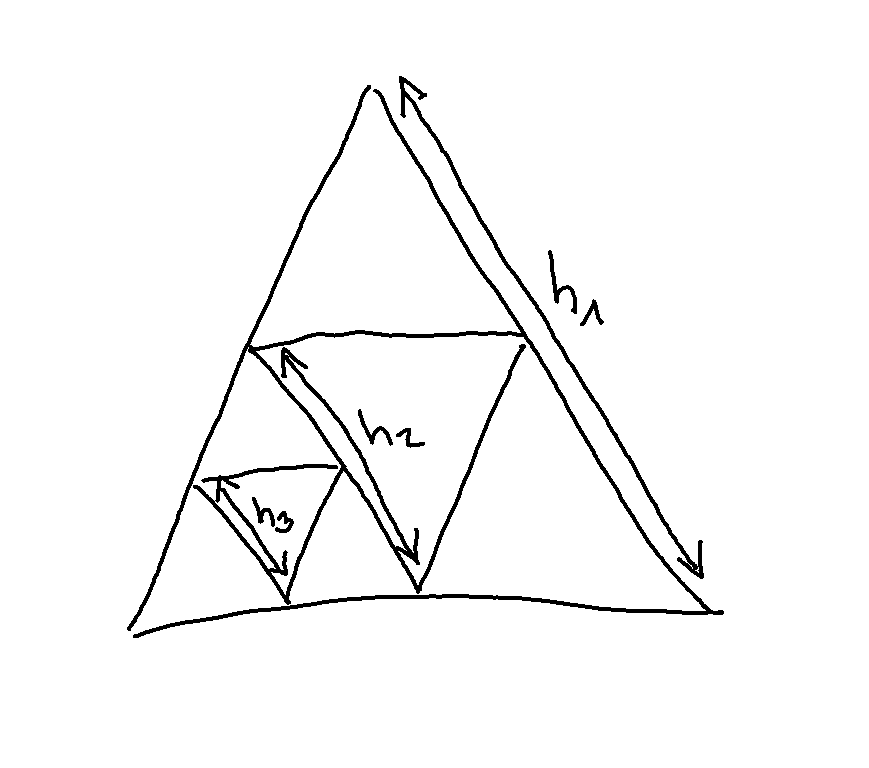
\includegraphics[width=0.75\textwidth]{pics/Sketch3.png}
				\caption{Beispielhafte Verfeinerung der Triangulierung mit einhergehender Konvergenz des Familienparameters}
				\label{AbbFamilienparameterKonvergenz}
			\end{center}
		\end{figure}
	\end{enumerate}
\end{definition}

\begin{theorem}\label{theorem4.16}
	Für eine formreguläre Familie von Finiten-Elementen $(K,V,\Sigma)$, alle affin-äquivalent zu $(\hat{K},\hat{V},\hat{\Sigma})$, ist die Abschätzung
	\begin{align*}
		\big| v-I_K v\big|\leq\tilde{c}\cdot\big(\meas(K)\big)^{\frac{1}{q}-\frac{1}{p}}\cdot h_K^{r+1-m}\cdot|v|_{r+1,p,K}
	\end{align*}
	erfüllt unter den Voraussetzungen von Theorem \ref{theorem4.14}. Außerdem gilt die Abschätzung dann für die Norm anstelle der Semi-Norm:
	\begin{align*}
		\big\Vert v-I_K v\big\Vert\leq\tilde{c}\cdot\big(\meas(K)\big)^{\frac{1}{q}-\frac{1}{p}}\cdot h_K^{r+1-m}\cdot|v|_{r+1,p,K}
	\end{align*}
\end{theorem}

\begin{theorem}\label{theorem4.17}
	Sei $V:=H_0^1(\Omega)$, $V_h\subseteq V$ ein Raum von Finiten Elementen auf $\T_h$ (gehörend zu einer formregulären Familie)  und seien $(K,V,\Sigma)$ affin-äquivalent zu $(\hat{K},\hat{V},\hat{\Sigma})$.\\
	Weiterhin sei $a$ eine koerzive, stetige Bilinearform auf $V$ und $l$ eine stetige Linearform auf $V$.
	Außerdem seien $u\in V$ und $u_h\in V_h$ die 	eindeutigen Lösungen des Variationsproblems auf $V$ bzw. $V_h$.
	Zusätzlich seien $\hat{N}_i\in\hat{\Sigma}$ stetig auf $H^{r+1}(\hat{K})$ und $P_r(\hat{K})\subseteq\hat{V}\subseteq H^1(\hat{K})$\\
	Dann gibt es eine Konstante $c$, unabhängig von $h$ so, dass
	\begin{align*}
		\Vert u-u_h\Vert_{1,2,\Omega}\leq c\cdot h^r\cdot|u|_{r+1,2,\Omega}
	\end{align*}
	unter der Voraussetzung, dass
	\begin{align*}
		u\in H^1_0(\Omega)\cap H^{r+1}(\Omega).
	\end{align*}
\end{theorem}

\begin{proof}
	Céa's Lemma \ref{theorem2.2CeasLemma} liefert
	\begin{align*}
		\Vert u-u_h\Vert_{1,2,\Omega}&\leq c\cdot \inf\limits_{v_h\in V_h}\Vert u-v_h\Vert_{1,2,\Omega}
		\leq c\cdot\Vert u-I_h u\Vert_{1,2,\Omega}
	\end{align*}
	Mit Theorem \ref{theorem4.16} folgt mit $m=1,p=q=2$ dann die Lokalisierungseigenschaft
	\begin{align*}
		\big(I_h v\big)\big|_K&=I_K\big(v|_K\big)\\
		\implies
		\big\Vert u-I_K u\big\Vert_{1,2,K}&\leq c\cdot h_K^r\cdot|u|_{r+1,2,K}\\
		\implies
		\big\Vert u-I_h u\big\Vert^2_{1,2,\Omega}
		&=\sum\limits_{K\in\T_h}\big\Vert u-I_h u\big\Vert^2_{1,2,K}\\
		&=\sum\limits_{K\in\T_h}\big\Vert u-I_K u\big\Vert^2_{1,2,K}\\
		&\leq
		c\cdot\sum\limits_{K\in\T_h}\underbrace{h_K^{2\cdot r}}_{\leq h^{2\cdot r}}\cdot|u|^2_{r+1,2,K}\\
		&\leq c\cdot h^{2\cdot r}\cdot\underbrace{\sum\limits_{K\in\T_h}|u|^2_{r+1,2,K}}_{=|u|^2_{r+1,2,\Omega}}\\
		&=c\cdot h^{2\cdot r}\cdot|u|^2_{r+1,2,\Omega}
	\end{align*}
\end{proof}

\begin{theorem}\label{theorem4.18}
	Zusätzlich zu den Voraussetzungen von Theorem \ref{theorem4.17} nehmen wir hier noch an, dass das Problem
	\begin{align*}
		\text{Finde }\varphi\in V\text{ so, dass }a(v,\varphi)=(g,v)~\forall v\in V.
	\end{align*}
	%provides?
	für alle $g\in L^2(\Omega)$ eine eindeutige Lösung $\varphi_g\in H^2(\Omega)$ hat, die
	\begin{align*}
		\Vert\varphi_g\Vert_{2,2,\Omega}\leq c\cdot\Vert g\Vert_{0,2,\Omega}
	\end{align*}
	erfüllt. Dann existiert eine Konstante $c$, unabhängig von $h$ so, dass
	\begin{align*}
		\Vert u-u_h\Vert_{0,2,\Omega}\leq c\cdot h^{r+1}\cdot|u|_{r+1,2,\Omega}
	\end{align*}
	falls $u\in H^{r+1}(\Omega)$.
\end{theorem}

\begin{proof}
	Nutze Theorem \ref{theorem2.3AubinNitscheDualitaetsargument} mit $H=L^2(\Omega),V=H_0^1(\Omega)$:
	\begin{align*}
		\Vert u-u_h\Vert_{0,2,\Omega}
		&\leq c\cdot\underbrace{\Vert u-u_h\Vert_{1,2,\Omega}}_{\leq c \cdot h^r\cdot|u|_{r+1,2,\Omega}}\cdot\sup\limits_{\begin{subarray}{c}g\in L^2(\Omega)\\\Vert g\Vert_{0,2,\Omega}=1\end{subarray}}\inf\limits_{v_h\in V_h}\Vert\varphi_g-v_h\Vert_{1,2,\Omega}
	\end{align*}
	\begin{align*}
		\implies
		\inf\limits_{v_h\in V_h}\Vert\varphi_g-v_h\Vert_{1,2,\Omega}
		&\leq\big\Vert\varphi_g -I_h\varphi_g\big\Vert_{1,2,\Omega}\\
		&\leq c\cdot h\cdot|\varphi_g|_{2,2,\Omega}\\
		&\leq c\cdot h\cdot\underbrace{\Vert g\Vert_{0,2,\Omega}}_{=1}
	\end{align*}
	\begin{align*}
		\implies
		\sup\limits_{\begin{subarray}{c}g\in L^2(\Omega)\\\Vert g\Vert_{0,2,\Omega}=1\end{subarray}}\inf\limits_{v_h\in V_h}\Vert\varphi_g-v_h\Vert_{1,2,\Omega}
		\leq c\cdot h
	\end{align*}
\end{proof}

Diese Abschätzungen ist eine \textbf{a priori Abschätzung}, d.h. man kann ohne Berechnungen Aussagen machen.

\begin{lemma}[Inverse Abschätzung]\label{lemma4.19InverseAbschaetzung}\enter
Sei $\lbrace V_h\rbrace$ eine Familie von affin-äquivalenten, formregulären Finiten-Elementen.\\
Dann gibt es eine konstante $c$, unabhängig von $h$, so, dass
	\begin{align*}
		|w_h|_{1,2,K}\leq c\cdot h^{-1}_K\cdot\Vert w_h\Vert_{0,2,K}\qquad\forall w\in V_h
	\end{align*}
	Global erhalten wir
	\begin{align*}
		|w_h|_{1,2,\Omega}\leq c\cdot h^{-1}_{\min}\cdot\Vert w_h\Vert_{0,2,\Omega}\qquad\forall w\in V_h
	\end{align*}
	wobei $h_{\min}:=\min\limits_{K\in\T_h} h_K$
\end{lemma}

\begin{proof}
	\begin{align*}
		|w_h|_{1,2,K}
		\overset{\ref{theorem4.9}}&{\leq}
		c\cdot\underbrace{\Vert B_K^{-1}\Vert^1}_{\leq h_K^{-1}}\cdot\big|\det(B_K)\big|^{\frac{1}{2}}\cdot\big|\underbrace{\hat{w}}_{=w_h\circ F_K}\big|_{1,2,\hat{K}}\\
		|\hat{w}_h|_{1,2,\hat{K}}
		&\leq \Vert\hat{w}\Vert_{1,2,\hat{K}}
		\stackrel{(\ast)}{\leq}
		c\cdot\Vert\hat{w}_h\Vert_{0,2,\hat{K}}\\
		\implies
		|w_h|_{1,2,K}
		&\leq c\cdot h_K^{-1}\cdot\big|\det(B_K)\big|^{\frac{1}{2}}\cdot\Vert\hat{w}_h\Vert_{0,2,\hat{K}}\\
		&\leq c\cdot h_K^{-1}\cdot\big|\det(B_K)\big|^{\frac{1}{2}}\cdot\underbrace{\Vert B_K\Vert^0}_{=1}\cdot\big|\det(B_K)\big|^{-\frac{1}{2}}\cdot\Vert w_h\Vert_{0,2,K}\\
		&= c\cdot h_K^{-1}\cdot\Vert w_h\Vert_{0,2,K}
	\end{align*}
	Bei ($\ast$) wird die Normäquivalenz auf endlichen-dimensionalen $\hat{V}$ benutzt.
\end{proof}
	% This work is licensed under the Creative Commons
% Attribution-NonCommercial-ShareAlike 4.0 International License. To view a copy
% of this license, visit http://creativecommons.org/licenses/by-nc-sa/4.0/ or
% send a letter to Creative Commons, PO Box 1866, Mountain View, CA 94042, USA.
% vim: set noexpandtab:

\section{Nichtkonforme Methoden} %5
\textbf{Nichtkonform} bedeutet: $V_h\not\subseteq V$\\
\textbf{Konform} bedeutet: $V_h\subseteq V$\\
Warum nichtkonforme Methoden?
\begin{enumerate}[label=(\roman*)]
	\item Probleme höherer Ordnung, z. B. von 4. Ordnung
	\begin{align*}
		V=H^2(\Omega)\qquad\qquad%\\
		\text{Konformität}\implies V_h\subseteq C^1
	\end{align*}
\item Skizze für Zerlegung des Gebietes in vier Teilgebiete, siehe Abbildung \ref{AbbNonconformingMethods}
	\begin{figure}[!ht]
		\begin{center}
			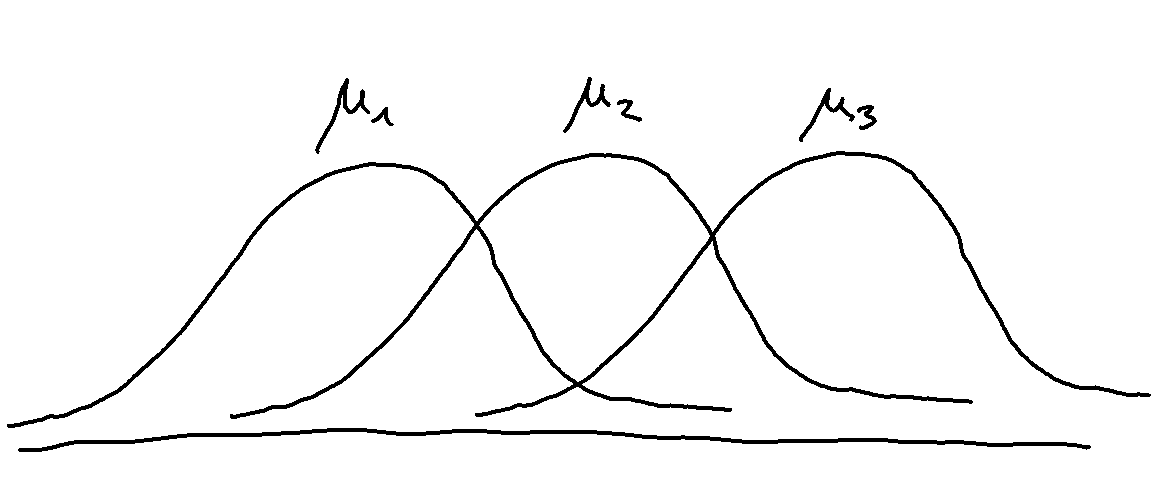
\includegraphics[width=0.75\textwidth]{pics/Sketch5.png}
			\caption{links: konformes $P_1$, rechts nichtkonformes $P_1$}
			\label{AbbNonconformingMethods}
		\end{center}
	\end{figure}
	\item Probleme mit Restriktionen/ Einschränkungen
\end{enumerate}

\subsection{Das nichtkonforme \texorpdfstring{$P_1$}{P\_1}-Element}
Alternative Bezeichnung: Crouzeix-Raviart, 1973\\
Definition lokaler Finite-Elemente $(K,V,\Sigma)$
\begin{align*}
	K&=\text{Dreieck oder Tetraeder}\\
	V&=P_1(K)=\spann\{1,x,y\}\text{ oder }\spann\{1,x,y,z\}\\
	\Sigma&=\big\{N_1,N_2,N_3\big\}\text{ oder }\big\lbrace N_1,N_2,N_3,N_4\big\rbrace\\
	N_i&:\text{ Integral-Mittelwert der Funktionen auf Kanten}\\
	&\text{(äquivalente Alternative: Funktionswerte auf den Mittelpunkten)}
\end{align*}

\begin{beisp}\enter
	\begin{figure}[!ht]
		\begin{center}
			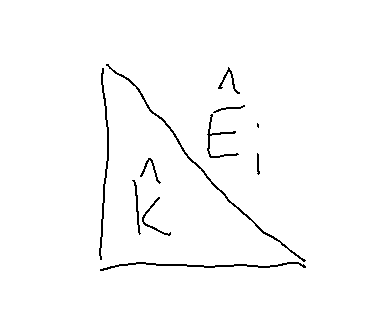
\includegraphics[width=0.25\textwidth]{pics/Sketch6.png}
			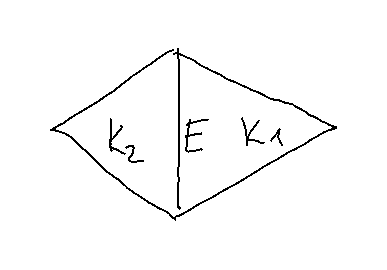
\includegraphics[width=0.25\textwidth]{pics/Sketch7.png}
			\caption{links Referenzdreieck mit Außenkante, rechts Dreiecke mit Innenkante}
			\label{AbbKantentypen}
		\end{center}
	\end{figure}
	\begin{align*}
		\hat{N}_i(\hat{v})=\frac{1}{|\hat{E}_i|}\cdot\int\limits_{\hat{E}_i}\hat{v}\d\gamma
	\end{align*}
\end{beisp}

Der Raum der Finiten-Elemente $V_h$ ist hierbei
\begin{align*}
	V_h=\left\lbrace v\in L^2(\Omega):
	\begin{array}{l}
		v|_K\in P_1(K), \\
		\int\limits_E [v]_E\d\gamma=0~\forall
		\text{ inneren Kanten $E$},\\
		\frac{1}{|E|}\cdot\int\limits_E v\d\gamma=0~\forall\text{ äußeren Kanten }E
	\end{array}
	\right\rbrace
\end{align*}
Hierbei ist $[v]_E$ der Sprung von $v$ über Kanten $E$.\\
\ul{Beobachtung}: Raum der stetigen, stückweise linearen Funktionen ist eine Teilmenge von $V_h$ mit Nullrandbedingungen (d.h. die Funktionen verschwinden auf dem Rand). Es folgt
\begin{align*}
	\inf\limits_{v_h\in V_h}\big\Vert u-v_h\big\Vert_{0,2,\Omega}
	\leq\inf\limits_{w_h\in S_{h,0}^{1,0}}\big\Vert u-w_h\big\Vert_{0,2,\Omega}
	\leq c\cdot h^2\cdot|u|_{2,2,\Omega}
\end{align*}
Wegen $V_h\not\subseteq V$ brauchen wir die Verallgemeinerung von $|\cdot|_{1,2,\Omega}$ für $v\in V=H^1_0(\Omega)$:
\begin{align*}
	|v|_{1,2,\Omega}^2
	&=\sum\limits_{K\in\T_h}|v|^2_{1,2,K}
	=\sum\limits_{K\in\T_h}\Big| v|_K\Big|^2_{1,2,K}
\end{align*}
Definiere
\begin{align*}
	|v|_{1,h}:=\left(\sum\limits_{K\in\T_h}|v|^2_{1,2,K}\right)^{\frac{1}{2}}
\end{align*}
Ist $|\cdot|_{1,h}$ eine Norm auf $V_h$? Es reicht die Null-Eigenschaft zu prüfen:
\begin{align*}
	|v_{1,h}|=0\implies v|_K=\text{konst.}
	\stackrel{\int\limits_E[v]_E\d\gamma=0}{\implies}
	v=\text{konst. auf }\Omega
	\stackrel{\int\limits_{E\in\Gamma} v\d\gamma=0}{\implies}
	v\equiv 0
\end{align*}
Folglich ist es wirklich eine Norm. Es gilt außerdem:
\begin{align*}
	\inf\limits_{v_h\in V_h}\big|u-v_h\big|_{1,h}
	\leq\inf\limits_{w_h\in S_{h,0}^{1,0}}\underbrace{\big|u-w_h\big|_{1,h}}_{|u-w_h|_{1,2}}
	\leq c\cdot h\cdot|u|_{2,2}
\end{align*}

\subsection{Abstraktes Framework}
Wir betrachten unser Modellproblem:
\begin{align*}
	\left\lbrace\begin{array}{rl}
		-\Delta u=f&\text{ in }\Omega\\
		u=0& \text{ auf }\Gamma=\partial\Omega
	\end{array}\right.
\end{align*}
Variationsformulierung: Finde $u\in V=H_0^1(\Omega)$ so, dass
\begin{align*}
	\underbrace{\int\limits_\Omega\nabla u\cdot\nabla v\d x}_{=:a(u,v)}=\underbrace{\int\limits_\Omega f\cdot v\d x}_{=:(f,v)}\qquad\forall v\in V
\end{align*}
Schwierigkeit: $a$ ist nicht definiert für alle Funktionen aus $V_h$. Setze
\begin{align*}
	a_h(v_h,w_h):=\sum\limits_{K\in\mathcal{T}_h}\int\limits_K\nabla v_h\cdot\underbrace{\nabla w_h}_{=\nabla(w_h|_K)}\d x
\end{align*}
Diskretes Problem: Finde $u_h\in V_h$ so, dass
\begin{align*}
	a_h(u_h,v_h)=(f,v_h)\qquad\forall v_h\in V_h
\end{align*}

\textbf{Annahmen:}
\begin{itemize}
	\item $V$ sei ein Hilbertraum
	\item $V_h$ sei ein diskreter Finite-Elemente-Raum mit Norm $\Vert\cdot\Vert_h$
	\item $a\colon V\times V\to\R$ sei ein stetige, $V$-elliptische Bilinearform
	\item $f\colon V\to\R$ sei linear und stetig
\end{itemize}
Dann sagt Lax-Milgram \ref{theorem2.1LaxMilgram}: Es existiert genau ein $u\in V$, welches das Problem löst.\nl
\textbf{Weitere Annahmen:}
\begin{itemize}
	\item $a_h$ sei eine Bilinearform auf $V+ V_h$ %kein Plan warum er hier $V+V_h$ schreibt. Ich ziehe das mal konsequent durch.
	\item $a_h$ sei \textbf{gleichmäßig stetig auf $V+ V_h$}, d. h.
	\begin{align*}
		\exists M>0\text{ unabhängig von }h:\big|a_h(u,v)\big|\leq M\cdot\Vert u\Vert_h\cdot\Vert v\Vert_h\qquad\forall u,v\in V+ V_h
	\end{align*}
	\item $f_h\colon V_h + V\to\R$ sei linear und stetig % orig: \cup, aber warum, wir haben doch überall + ?!
	\item $a_h$ ist \textbf{gleichmäßig $V_h$-elliptisch}, d.h.
	\begin{align*}
		\alpha\cdot\Vert v_h\Vert^2_h\leq a_h(v_h,v_h)\qquad\forall v_h\in V_h
	\end{align*}
	wobei $\alpha$ unabhängig von $v_h$ und $h$ ist.
\end{itemize}
Dann sagt Lax-Milgram \ref{theorem2.1LaxMilgram}: Es existiert genau ein $u_h\in V_h$, welches das Problem löst. Welcher Zusammenhang besteht nun zwischen $u$ und $u_h$?

\begin{theorem}[Zweites Lemma von Strang]\label{theorem5.1ZweitesLemmaStrang}\enter
	Sei $\lbrace V_h\rbrace$ eine Familie von (nichtkonformen) Finiten-Elementen-Räumen. Bezeichne $u$ und $u_h$ die schwache bzw. die diskrete Lösung. Dann gilt:
	\begin{align*}
		\big\Vert u-u_h\big\Vert_h\leq\left(1+\frac{M}{\alpha}\right)\cdot\inf\limits_{v_h\in V_h}\big\Vert u-v_h\big\Vert_h
		+\frac{1}{\alpha}\cdot\sup\limits_{z_h\in V_h}\frac{a_h(u,z_h)-f_h(z_h)}{\Vert z_h\Vert_h}
	\end{align*}
	Hierbei ist erste Summand auf der rechten Seite der Approximationsfehler und der zweite Term der Konsistenzfehler.
\end{theorem}

\begin{bemerkung}
	konforme Methode: $V_h\subseteq V,~a_h=a,f_h=f$ und damit:
	\begin{align*}
		a_h(u,z_h)-f_h(z_h)=a(u_h,z_h)-f(z_h)=0\text{ wegen } z_h\in V_h\subseteq V
	\end{align*}
	Folglich gibt es im Fall der konformen Methode keinen Konsistenzfehler.
\end{bemerkung}

\begin{proof}
	Sei $v_h\in V_h$ beliebig, $w_h\coloneqq v_h-u_h$. Dann gilt:
	\begin{align*}
		α \norm{v_h-u_h}_h^2
		&\leq a_h\big(v_h-u_h,v_h-u_h\big) = a_h\big(v_h-u_h, w_h\big)\\
		&=a_h\big(v_h,w_h\big)-\underbrace{a_h\big(u_h,w_h\big)}_{=f_h(w_h)}\\
		&=a_h\big(v_h-u,w_h\big)+a_h\big(u,w_h\big)-f_h\big(w_h\big)\cdot\frac{\Vert w_h\Vert_h}{\Vert w_h\Vert_h}\\
		&\leq M\cdot\big\Vert v_h-u\big\Vert_h\cdot\big\Vert w_h\big\Vert_h+\Vert w_h\Vert_h\cdot\sup\limits_{z_h\in V_h}\frac{a_h\big(u,z_h\big)-f_h\big(z_h\big)}{\Vert z_h\Vert_h}\\
		\implies
		\underbrace{\norm{w_h}_h}_{=\norm{v_h-u_h}_h}
		&\leq\frac M{α} · \norm{v_h-u}_h
		+ \frac1{α} · \sup_{z_h ∈ V_h} \frac{a_h\big(u,z_h\big)-f_h\big(z_h\big)}{\norm{z_h}_h}
	\end{align*}
	Mit der Dreicksungleichung folgt:
	\begin{align*}
		\norm{u-u_h}_h
		&\leq \norm{u-v_h}_h + \norm{v_h-u_h}_h\\
		&\leq\left(1+\frac{M}{\alpha}\right)\cdot\Vert u-v_h\Vert_h+\frac{1}{\alpha}\cdot\sup\limits_{z_h\in V_h}\frac{a_h\big(u,z_h\big)-f_h\big(z_h\big)}{\Vert z_h\Vert_h}
	\end{align*}
	Bilden des Infimums $\inf\limits_{v_h\in V_h}$ liefert die Behauptung.
\end{proof}

\subsection{Überprüfen der Voraussetzungen für das Poisson-Problem}
\begin{align*}
	a_h(v_h,w_h)&=\sum\limits_{K\in\T_h}\int\limits_K\nabla v_h\cdot\nabla w_h\d x\\
	f_h(v_h)&=\sum\limits_{K\in\T_h}\int\limits_K f\cdot v_h\d x\\
	\Vert v\Vert_h&=\left(\sum\limits_{K\in\T_h}|v|_{1,2,K}\right)^{\frac{1}{2}}
\end{align*}
$\Vert\cdot\Vert_h$ ist eine Norm auf $V+ V_h$.\\
Gleichmäßige Stetigkeit von $a_h$ auf $V+ V_h$: Seien $v,w\in V\cup V_h$. Dann gilt:
\begin{align*}
	\big|a_h(v,w)\big|
	&=\left|\sum\limits_{K\in\T_h}\int\limits_K\nabla v\cdot\nabla w\d x\right|\\
	\overset{\text{CS}}&\leq
	\sum\limits_{K\in\T_h}|v|_{1,2,K}\cdot |w|_{1,2,K}\\
	\overset{\text{CS}}&\leq
	\left(\sum\limits_{K\in\T_h} |v|_{1,2,K}^2\right)^{\frac{1}{2}}\cdot\left(\sum\limits_{K\in\T_h}|w|_{1,2,K}^2\right)^{\frac{1}{2}}\\
	&=\Vert v\Vert_h\cdot\Vert w\Vert_h \quad
	(\implies M=1)
\end{align*}
Gleichmäßige $V_h$-Elliptizität von $a_h$ auf $V_h$: Sei $v_h\in V_h$ beliebig. Dann gilt:
\begin{align*}
	a_h(v_h,v_h)
	&=\sum\limits_{K\in\T_h}\int\limits_K\nabla v_h\cdot\nabla v_h\d x
	=\sum\limits_{K\in\T_h}|v_h|^2_{1,2,K}
	=\Vert v_h\Vert^2_h \quad
	(\implies\alpha=1)
\end{align*}
Stetigkeit von $f_h$ auf $V_h$:
\begin{align*}
	\big|f_h(v_h)\big|
	&=\left|\sum\limits_{K\in\T_h}\int\limits_K f\cdot v_h\d x\right|
	\overset{\text{}}\leq
	\sum\limits_{K\in\T_h}\Vert f \Vert_{0,2,K}\cdot\Vert v_h\Vert_{0,2,K}
	\overset{\text{}}\leq
	\Vert f\Vert_{0,2,\Omega}\cdot\Vert v_h\Vert_{0,2,\Omega}
\end{align*}
Auf $V_h$ (endlich-dimensionaler Raum) sind die Normen $\Vert\cdot\Vert_h$ und $\Vert\cdot\Vert_{0,2,\Omega}$ äquivalent:
\begin{align*}
	\implies
	\big|f_h(v_h)\big|
	\leq
	c_h\cdot\Vert f\Vert_{0,2,\Omega}\cdot\Vert v_h\Vert_h
\end{align*}

\subsection{Fehlerabschätzung} %5.4
Bisher:
\begin{align*}
	\Vert u-u_h\Vert_h
	&\leq
	2\cdot\underbrace{\inf\limits_{v_h\in V_h}\Vert u-v_h\Vert_h}_{\leq c\cdot h\cdot |u|_{2,2}}+1\cdot\underbrace{\sup\limits_{z_h\in V_h}\frac{a_h(u,z_h)-f_h(z_h)}{\Vert z_h\Vert_h}}_{\leq?}
\end{align*}
Sei $f\in L^2(\Omega)$ und $u\in H^2(\Omega)$. Dann:
\begin{align*}
	-\laplace u=f \text{ im $L^2$-Sinn auf jedem } K ∈ \T_h
\end{align*}
Sei nun $z_h\in V_h$ beliebig. Dann gilt:
\begin{align*}
	Σ_{K∈\T_h}∫\limits_K-\laplace u · z_h\d x
	&=Σ_{K∈\T_h}∫\limits_K f · z_h\d x\\
	Σ_{K∈\T_h}∫\limits_K-\laplace u · z_h\d x
	\overset{\text{part. Int.}}&=
	Σ_{K∈\T_h}\left(∫\limits_K∇ u · ∇ z_h\d x-∫\limits_{\Rand K}\underbrace{\frac{∂ u}{∂ n_K}}_{=∇ u · n_K}z_h\d γ \right)\\
	\implies L_h(z_h)
	&\coloneqq a_h(u,z_h)-f_h(z_h)\\
	&=Σ_{K∈\T_h}∫\limits_{\Rand K}\frac{∂ u}{∂ n_K}z_h\d γ \\
	&=Σ_{E}∫\limits_E\underbrace{\left[\frac{∂ u}{∂ u_E}z_h\right]_E}_{=\frac{∂ u}{∂ u_E}[z_h]_E}\d γ \\
	&=Σ_E∫\limits_E\frac{∂ u}{∂ u_E}[z_h]_E\d γ \\
	\text{wobei } [v]_E &\coloneqq v|_{K_1}-v|_{K_2}
\end{align*}
\begin{figure}[!ht]
	\begin{center}
		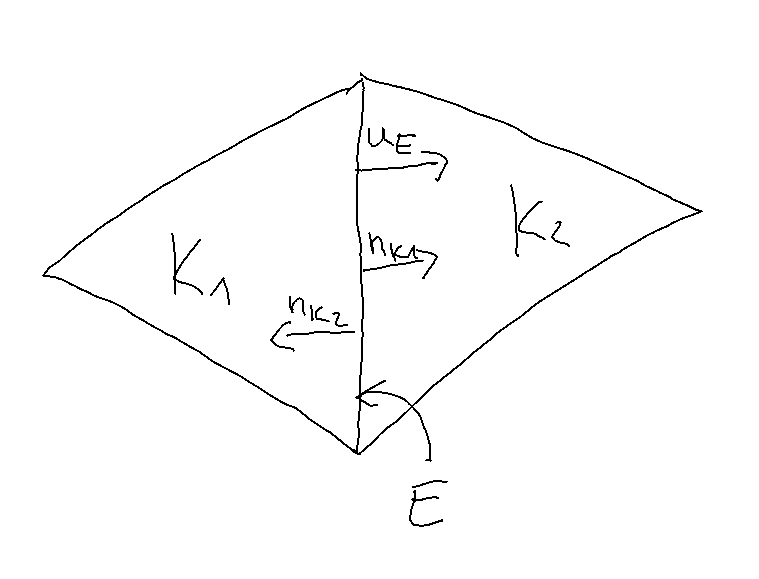
\includegraphics[width=0.75\textwidth]{pics/Sketch8.png}
		\caption{Skizze der Normalen an Kante zwischen zwei Dreiecken}
		\label{AbbNormalvectors}
	\end{center}
\end{figure}
Seien $\overline{z}_h$ und $\overline{\frac{\partial u}{\partial u_E}}$ die konstanten Integral-Mittelwerte von $z_h$ und $\frac{\partial u}{\partial u_E}$ auf jedem $E$, formal:
\begin{align*}
	\overline{z}_h|_E
	:&=\frac{1}{|E|}\cdot\int\limits_E z_h\d\gamma,\qquad\left.\overline{\frac{\partial u}{\partial u_E}}\right|_E \coloneqq \frac{1}{|E|}\cdot\int\limits_E \frac{\partial u}{\partial u_E}\d\gamma
\end{align*}
Mit
\begin{align*}
	\int\limits_E[z_h]_E\d\gamma=0\text{ wegen }z_h\in V_h
\end{align*}
und da $\overline{\frac{\partial u}{\partial u_E}}$ eine Konstante ist
folgt
\begin{align*}
	\int\limits_E\frac{\partial u}{\partial u_E}[z_h]_E\d\gamma
	&=\int\limits_E\left(\frac{\partial u}{\partial u_E}-\overline{\frac{\partial u}{\partial u_E}}\right)[z_h]_E\d\gamma
	=\int\limits_E\left(\frac{\partial u}{\partial u_E}-\overline{\frac{\partial u}{\partial u_E}}\right)[z_h-\overline{z}_h]_E\d\gamma\\
	\implies
	L_h(z_h)
	&=\sum\limits_{K\in\T_h}\sum\limits_{E\subseteq\partial K}\int\limits_E\left(\frac{\partial u}{\partial u_E}-\overline{\frac{\partial u}{\partial u_E}}\right)\big[z_h-\overline{z}_h\big]_E\d\gamma\\
	\overset{\text{CS}}&\leq
	\sum\limits_{K\in\T_h}\sum\limits_{E\subseteq\partial K}\left\Vert\frac{\partial u}{\partial u_E}-\overline{\frac{\partial u}{\partial u_E}}\right\Vert_{0,2,E}\cdot\Vert z_h-\overline{z}_h\Vert_{0,2,E}
\end{align*}
Berechne nun für die Differenz: $z_h-\overline{z}_h$:
\begin{align*}
	\big\Vert z_h-\overline{z}_h\big\Vert_{0,2,E}
	&\leq
	c\cdot\underbrace{\big\Vert B_E^{-1}\big\Vert^0}_{=1}\cdot{\underbrace{\big|\det(B_E)\big|}_{=h_E}}^{\frac{1}{2}}\cdot\big\Vert \underbrace{\hat{z}_h-		\hat{\overline{z}}_h}_{=\widehat{z_h-\overline{z}_h}}\big\Vert_{0,2,\hat{E}}\\
	&\leq
	c\cdot h_E^{\frac{1}{2}}\cdot\big\Vert\widehat{z_h-\overline{z}_h}\big\Vert_{0,2,\hat{E}}
\end{align*}
Der Operator
\begin{align*}
	L\colon H^1(\hat{K})\to L_2(\hat{E}),\qquad\hat{v}\mapsto\left(\hat{v}-\overline{\hat{v}}\right)|_{\hat{E}}
	\mit \overline{\hat{v}}=\frac{1}{|\hat{E}|}\cdot\int\limits_{\hat{E}}\hat{v}\d\gamma
\end{align*}
ist linear und stetig. Folglich gilt:
\begin{align*}
	\big\Vert L(\hat{v})\big\Vert_{0,2,\hat{E}}
	&=\big\Vert\hat{v}-\overline{\hat{v}}\big\Vert_{0,2,\hat{E}}
	\leq
	\underbrace{\Vert\hat{v}\Vert_{0,2,\hat{E}}}_{\stackrel{\text{Spursatz}}{\leq} c\cdot\Vert\hat{v}\Vert_{1,2,\hat{K}}}+\big\Vert\overline{\hat{v}}\big		\Vert_{0,2,\hat{E}}\\
	\big\Vert\overline{\hat{v}}\big\Vert^2_{0,2,\hat{E}}
	&=
	\int\limits_{\hat{E}}\big|\overline{\hat{v}}\big|^2\d\gamma \\
	&=
	\left(\frac{1}{|\hat{E}|}\cdot\int\limits_{\hat{E}}\hat{v}\d\gamma\right)^2\cdot|\hat{E}|\\
	&\leq
	\frac{1}{|\hat{E}|^2}\cdot\Big(\underbrace{\Vert1\Vert_{0,2,\hat{E}}}_{=|\hat{E}|^{\frac{1}{2}}}\cdot\Vert\hat{v}\Vert_{0,2,\hat{E}}\Big)^2\cdot|\hat{E}|\\
	&=\Vert\hat{v}\Vert^2_{0,2,\hat{E}}\\
	&\leq c\cdot\Vert\hat{v}\Vert_{1,2,\hat{K}}
\end{align*}
Somit:
\begin{align*}
	\implies
	\big\Vert L(\hat{v})\big\Vert_{0,2,\hat{E}}
	&\leq c\cdot\Vert\hat{v}\Vert_{1,2,\hat{K}}
\end{align*}
Außerdem
\begin{align*}
	%\implies
	L(\hat{w})&=0\qquad\forall\hat{w}\in P_0(\hat{K})\\
	\overset{\text{Bramble-Hilbert}}{\implies}
	\big\Vert L(\hat{v})\big\Vert_{0,2,\hat{E}}
	&\leq
	c\cdot|\hat{v}|_{1,2,\hat{K}}\\
	\implies
	\big\Vert z_h-\overline{z}_h\big\Vert_{0,2,E}
	&\leq c\cdot h_E^{\frac{1}{2}}\cdot\big|\hat{z}_h\big|_{1,2,\hat{K}}\\
	\overset{\text{transf. zurück}}&{\leq}
	c\cdot h_E^{\frac{1}{2}}\cdot\underbrace{\Vert B_K\Vert^1}_{\sim h_K}\cdot{\underbrace{\big|\det(B_K)\big|}_{\sim h_K^2}}^{-\frac{1}{2}}\cdot|z_h|_{1,2,K}\\
	&\leq
	c\cdot h_E^{\frac{1}{2}}\cdot|z_h|_{1,2,K}
\end{align*}
Auf ähnliche Art und Weise, aber mit wesentlich mehr Aufwand, erhält man auch:
\begin{align*}
	\left\Vert\frac{\partial u}{\partial u_K}-\overline{\frac{\partial u}{\partial u_K}}\right\Vert_{0,2,E}
	&\leq c\cdot h_E^{\frac{1}{2}}\cdot\Vert u\Vert_{2,2,K}
\end{align*}
Nun können wir endlich alle Abschätzungen zusammenbringen und erhalten
\begin{align*}
	\implies
	L_h(z_h)
	&\leq
	\sum\limits_{K\in\T_h}\sum\limits_{E\subseteq\partial K}\left\Vert\frac{\partial u}{\partial u_K}-\overline{\frac{\partial u}{\partial u_K}}\right\Vert_{0,2,E}\cdot\big\Vert z_h-\overline{z}_h\big\Vert_{0,2,E}\\
	&\leq
	c\cdot\sum\limits_{K\in\T_h} h^{\frac{1}{2}}\cdot\Vert u\Vert_{2,2,K}\cdot h^{\frac{1}{2}}\cdot|z_h|_{1,2,K}\\
	&\leq
	c\cdot h\cdot\left(\sum\limits_{K\in\T_h}\Vert u\Vert^2_{1,2,K}\right)^{\frac{1}{2}}\cdot\left(\sum\limits_{K\in\T_h}|z_h|_{1,2,K}^2\right)^{\frac{1}{2}}\\
	&=c\cdot h\cdot \Vert u\Vert_{2,2,\Omega}\cdot\Vert z_h\Vert_h\\
	\implies
	\sup\limits_{z_h\in V_h}\frac{a_h(u, z_h)-f_h(z_h)}{\Vert z_h\Vert_h}
	&\leq c\cdot h\cdot\Vert u\Vert_{2,2,\Omega}
\end{align*}

\begin{theorem}\label{theorem5.2}
	Sei $\lbrace V_h\rbrace$ eine Familie von $P_1$-nichtkonformen Finite-Elemente-Räume, wobei $u_h\in V_h$ das diskrete Problem löst und $u\in V\cap H^2(\Omega)$ die Lösung der schwachen Formulierung ist. Dann gilt:
	\begin{align*}
		\big\Vert u-u_h\big\Vert_h\leq c\cdot h\cdot\Vert u\Vert_{2,2,\Omega}
	\end{align*}
\end{theorem}

\begin{bemerkung}
	Das Dualitätsargument von Aubin und Nietsche kann erweitert werden auf den nichtkonformen Fall. Dabei tauchen zwei neue Terme in der Abschätzung auf.
	\begin{align*}
		\big\Vert u-u_h\big\Vert_{0,2,\Omega}\leq c\cdot h^2\cdot\Vert u\Vert_{2,2,\Omega}
	\end{align*}
\end{bemerkung}
	% This work is licensed under the Creative Commons
% Attribution-NonCommercial-ShareAlike 4.0 International License. To view a copy
% of this license, visit http://creativecommons.org/licenses/by-nc-sa/4.0/ or
% send a letter to Creative Commons, PO Box 1866, Mountain View, CA 94042, USA.
% vim: set noexpandtab:

\section{A posteriori Fehlerabschätzung} %6
Modellproblem: $\Omega\subseteq\R^2,f\in L^2(\Omega)$
\begin{align*}
	\left\lbrace\begin{array}{rl}
		-\Delta u=f &\text{ in }\Omega\\
		u=0 &\text{ auf }\Gamma=\partial\Omega
	\end{array}\right.
\end{align*}
Schwache Formulierung: Finde $u\in H_0^1(\Omega)$ so, dass
\begin{align*}\label{eqSection6P}\tag{$P$}
	\underbrace{\int\limits_\Omega\nabla u\cdot\nabla v\d x}_{=:a(u,v)}=\underbrace{\int\limits_\Omega f\cdot v\d x}_{=:l(v)}\qquad\forall v\in H_0^1(\Omega)
\end{align*}
Konforme Finite-Elemente-Diskretisierung:\\
Sei $\lbrace\T_h\rbrace$ eine Familie von Form-regulären Triangulierungen mit\\ Finiten-Elementen-Räumen $X_h$ von stetigen, stückweise $P_h$-polynomiellen Funktionen\nl
Diskretes Problem: Finde $u\in X_h$ so, dass
\begin{align}\label{eqSection6Ph}\tag{$P_h$}
	a(u_h,v_h)=l(v_h)\qquad\forall v_h\in X_h
\end{align}
Ziel: Finde berechenbare Schranken für den Fehler $u-u_h$ in irgendeiner Norm.

\subsection*{Informelle Definition}
\begin{itemize}
	\item Eine Menge $\eta$ heißt \textbf{(Posteriori-)Fehlerschätzer} $:\gdw\eta$ ist berechenbar aus den Problemdaten und der diskreten Lösung $u_h$.
	\item Ein Fehlerschätzer $\eta$ heißt \textbf{zuverlässig} $:\gdw$ es gibt eine obere Schranke für den globalen Fehler, d.h.
	\begin{align*}
		:\Longleftrightarrow\exists c\in\R:\big\Vert u-u_h\big\Vert_\Omega\leq c\cdot\eta
	\end{align*}
	Zuverlässige Fehlerschätzer sind nützlich um eine gewisse Genauigkeit sicherzustellen.
	\item Ein Fehlerschätzer $\eta$ heißt \textbf{effizient} $:\gdw$ es existiert eine lokale untere Schranke für den Fehler, d.h.
	\begin{align*}
		\eta_{\text{ lokal}}\leq c\cdot\big\Vert u-u_h\big\Vert_{\text{lokal}}+\text{Daten-Oszillation}
	\end{align*}
	Da wir später $f$ durch ein Approximationspolynom ersetzen, kommt ein Fehlerterm hinzu, welchen wir \textbf{Daten-Oszillation} nennen.\\
	Effiziente Fehlerschätzer soll eine Überschätzung der lokalen Verfeinerung verhindern.
\end{itemize}

\subsection*{Residuale Fehlerschätzer}
Aus der Friedrich-Ungleichung \ref{prop1.13FriedrichsUngleichung} folgt:
\begin{align*}
	a(v,v)&\geq\alpha\cdot\Vert v\Vert^2_{1,2,\Omega}\qquad\forall v\in H^1_0(\Omega)\\
	\implies
	\Vert u-u_h\Vert^2_{1,2,\Omega}
	&\leq
	\frac{1}{\alpha}\cdot a\big(u-u_h,u-u_h\big)\\
	\implies
	\Vert u-u_h\Vert_{1,2,\Omega}
	&\leq\frac{1}{\alpha}\cdot a\left(u-u_h,\frac{u-u_h}{\Vert u-u_h\Vert_{1,2,\Omega}}\right)\\
	\implies
	\Vert u-u_h\Vert_{1,2,\Omega}
	&\leq\frac{1}{\alpha}\cdot\sup\limits_{\begin{subarray}{c}v\in H^1_0(\Omega)\\\Vert v\Vert_{1,2,\Omega}=1\end{subarray}}\Big(\underbrace{a(u,v)}_{=l(v)}-a(u_h,v)\Big)
\end{align*}
Andererseits erhalten wir:
\begin{align*}
	\sup\limits_{\begin{subarray}{c}v\in H^1_0(\Omega)\\\Vert v\Vert_{1,2,\Omega}=1\end{subarray}} a(u-u_h,v)
	&\leq
	\sup\limits_{\begin{subarray}{c}v\in H^1_0(\Omega)\\\Vert v\Vert_{1,2,\Omega}=1\end{subarray}}
	\Vert u-u_h\Vert_{1,2,\Omega}\cdot\underbrace{\Vert v\Vert_{1,2,\Omega}}_{=1}
	=\Vert u-u_h\Vert_{1,2,\Omega}\\
\end{align*}
Also bekommen wir die Abschätzungen
\begin{align*}
	\sup\limits_{\begin{subarray}{c}v\in H^1_0(\Omega)\\\Vert v\Vert_{1,2,\Omega}=1\end{subarray}} a(u-u_h,v)
	&\leq
	\Vert u-u_h\Vert_{1,2,\Omega}
	\leq\frac{1}{\alpha}\cdot\sup\limits_{\begin{subarray}{c}v\in H^1_0(\Omega)\\\Vert v\Vert_{1,2,\Omega}=1\end{subarray}} a(u-u_h,v)
\end{align*}
Das bedeutet, dass die Norm $\Vert u_h-u\Vert_{1,2,\Omega}$ äquivalent zu der Operatornorm der linearen Abbildung
\begin{align*}
	R:H^1_0(\Omega)\to\R,\qquad v\mapsto l(v)-a(u_h,v)=a(u-u_h,v)
\end{align*}
ist. Beobachtung: Aus der Galerkin Orthogonalität folgt:
\begin{align*}
	R(v_h)=a(u-u_h,v_h)=0
\end{align*}
Für $v\in H^1_0(\Omega)\mit\Vert v\Vert_{1,2,\Omega}=1$ gilt:
\begin{align*}
	R(v)&=l(v)-a(u_h,v)\\
	&=\int\limits_\Omega f\cdot v\d x-\int\limits_\Omega\nabla u_h\cdot\nabla v\d x\\
	&=\sum\limits_{T\in\T_h}\left(\int\limits_T f\cdot v\d x-\int\limits_T \nabla u_h\cdot\nabla v\d x\right)\\
	&=\sum\limits_{T\in\T_h}\left(\int\limits_T f\cdot v\d x+\int\limits_T\Delta u_h\cdot v\d x-\int\limits_{\partial T}\nabla u_h\cdot u_T\cdot v\d\gamma\right)\\
	&=\sum\limits_{T\in\T_h}\int\limits_T\big(f+\Delta u_h\big)\cdot v\d x
	+\sum\limits_{E\in\mathcal{E}_h}\int\limits_E\big[\nabla u_h\cdot u_E\big]_E\cdot v\d\gamma\\
	\overset{\text{CS}}&\leq
	\sum\limits_{T\in\T_h}\big\Vert f+\Delta u_h\big\Vert_{0,2,T}\cdot\Vert v\Vert_{0,2,T}+\sum\limits_{E\in\mathcal{E}_h}\Big\Vert\big[\nabla u_h\cdot u_E\big]_E\Big\Vert_{0,2,E}\cdot\Vert v\Vert_{0,2,E}
\end{align*}
\begin{align*}
	R(v)
	&=R(v-v_h)\\
	&\leq
	\sum\limits_{T\in\T_h}\big\Vert f+\Delta u_h\big\Vert_{0,2,T}\cdot\Vert v-v_h\Vert_{0,2,T}
	&+\sum\limits_{E\in\mathcal{E}_h}\Big\Vert\big[\nabla u_h\cdot u_E\big]_E\Big\Vert_{0,2,E}\cdot\Vert v-v_h\Vert_{0,2,E}
\end{align*}
,wobei $\mathcal{E}_h$ die Menge aller Kanten ist.
\begin{align*}
	\text{Bester Weg}&: \text{Wähle $v_h$ als Interpolation von } v.\\
	\text{Aber}&: v\text{ ist nur in }H^1\text{ \& die gewöhnliche Interpolation wird nicht funktionieren.}\\
	\text{Lösung}&:\text{Quasi-Interpolation.}\\
	\text{Hier}&: \text{Quasi-Interpolation von Clément}
\end{align*}

\begin{notation}\
	\begin{itemize}
		\item $N_h$ ist die Menge Knoten.
		\item $N_{h,\Omega}$ ist die Menge aller Knoten in $\Omega$.
		\item $\varphi_z\in S^{1,0}_{h,0}$ sei stetig, stückweise lineare Hut-Funktion assoziiert zu $z\in N_h$
		\item $\overline{w}_z:=\inner\left(\bigcup\limits_{\begin{subarray}{c}T\in\T_h\\z\text{ ist Knoten von }T\end{subarray}}\overline{T}\right)$
		\item Für $v\in L^2(w_z)$ definiere die \textbf{$L^2$-Projektion auf Konstanten} durch
		\begin{align*}
			\pi_z (v):=\frac{1}{|w_z|}\cdot\int\limits_{w_z} v\d x
		\end{align*}
		\item Quasi-Interpolation von Clément:
		\begin{align*}
			R_h:H^1_0(\Omega)\to S^{1,0}_{h,0}\subseteq X_h,\qquad
			R_h(v):=\sum\limits_{z\in N_{h,\Omega}}\left(\pi_z(v)\right)\cdot\varphi_z
		\end{align*}
	\end{itemize}
\end{notation}

Als nächstes brauchen wir Abschätzungen für
\begin{align*}
	\big\Vert v-R_h(v)\big\Vert_{0,2,T}\qquad\text{und}\qquad\big\Vert v-R_h(v)\big\Vert_{0,2,E}
\end{align*}
gegen die $H^1$-Normen auf $v$.

\begin{theorem}[skalierter Spursatz]\label{theoremSkalierterSpursatz}\enter
	Sei $T\in\T_h$ und $E$ eine Kante von $T$.\\
	Dann existiert eine Konstante $c$, die nur von der Form-Regularitäts-Konstante abhängt, so dass
	\begin{align*}
		\Vert v\Vert_{0,2,E}\leq c\cdot\left(h_T^{-\frac{1}{2}}\cdot\Vert v\Vert_{0,2,T}+ h_T^{\frac{1}{2}}\cdot|v|_{1,2,T}\right)\qquad\forall v\in H^1(T)
	\end{align*}
\end{theorem}

Der Wert im Knoten $z$ ist
\begin{align*}
	\pi_z (v)=\frac{1}{|w_z|}\cdot\int\limits_{w_z}v\d x
\end{align*}
Es gilt
\begin{align*}
	\Vert v\Vert_{0,2,E}\leq c\cdot\left(h_T^{-\frac{1}{2}}\cdot\Vert v\Vert_{0,2,T}+h_T^{\frac{1}{2}}\cdot|v|_{1,2,T}\right)
\end{align*}

\begin{proof}
	Bezeichne $\hat{T}$ das Referenzdreieck mit Referenzkante $\hat{E}$. Außerdem sei $T$ ein beliebiges Dreieck mit Ecken $(a_1,b_1)$, $(a_2,b_2)$, $(a_3,b_3)$ und Kante $E$.
	Dann ist die Transformation zwischen beiden Dreiecken gegeben durch
	\begin{align*}
		F_T(\hat{x},\hat{y})=\begin{pmatrix}
			x\\y
		\end{pmatrix}
		&=\begin{pmatrix}
			a_1\\ b_1
		\end{pmatrix}
		+\hat{x}\cdot\begin{pmatrix}
			a_2-a_1\\ b_2-b_1
		\end{pmatrix}+
		\hat{y}\cdot\begin{pmatrix}
			a_3-a_1\\ b_3-b_1
		\end{pmatrix}\\
		&=\begin{pmatrix}
			a_1\\ b_1
		\end{pmatrix}
		+\underbrace{\begin{pmatrix}
			a_2-a_1 & a_3-a_1\\
			b_2-b_1 & b_3-b_1
		\end{pmatrix}}_{=:B_T}\cdot\begin{pmatrix}
			\hat{x}\\ \hat{y}
		\end{pmatrix}
	\end{align*}
	Mit
	\begin{align*}
		\varphi\colon[0,1]\to E,\quad\varphi(s):=\begin{pmatrix}
		a_1\\ b_1
		\end{pmatrix}+s\cdot\begin{pmatrix}
		a_2-a_1\\
		b_2-b_1
		\end{pmatrix},\quad
		\big\Vert\dot\varphi(s)\big\Vert=\left\Vert\begin{pmatrix}
		a_2-a_1\\
		b_2-b_1
		\end{pmatrix}\right\Vert=|E|=h_E
	\end{align*}
	folgt
	\begin{align*}
		&\Vert v\Vert_{0,2,E}^2
		=\int\limits_E|v|^2\d\gamma
		=\int\limits_0^1\Big|v\big(\varphi(s)\big)\Big|^2\cdot\big\Vert\dot{\varphi}(s)\big\Vert\d s
		=h_E\cdot\big\Vert\hat{v}\big\Vert_{0,2,\hat{E}}^2\\
	\end{align*}
	Demnach
	\begin{align*}
		&\big\Vert\hat{v}\big\Vert_{0,2,E}^2\\
		\overset{\ref{satz1.7Spursatz}}&\leq
		c\cdot h_E\cdot\Vert\hat{v}\Vert_{1,2,\hat{T}}^2
		=c\cdot h_E\cdot\left(\Vert\hat{v}\Vert_{0,2,\hat{T}}^2+\Vert\hat{v}\Vert_{1,2,\hat{T}}^2\right)\\
		\overset{\ref{theorem4.9}}&\leq
		c\cdot
		\underbrace{h_E}_{\leq h_T}\cdot\Bigg(c\cdot\underbrace{\Vert B_T\Vert^{0\cdot2}}_{=1}\cdot
		\underbrace{\big|\det(B_t)\big|^{-\frac{1}{2}\cdot2}}_{\leq c\cdot h_T^{-2}}\cdot\Vert v\Vert^2_{0,2,T}+c\cdot
		\underbrace{\Vert B_T\Vert^{1\cdot2}}_{\leq c\cdot h_T^2}\cdot
		\underbrace{\big|\det(B_T)\big|^{-\frac{1}{2}\cdot2}}_{c\cdot h^{-2}_T}\cdot|v|^2_{1,2,T}\Bigg)\\
		&\leq
		c\cdot\left(h_T^{-1}\cdot\Vert v\Vert_{0,2,T}^2+h_T\cdot|v|^2_{1,2,T}\right)
	\end{align*}
	% Das ist doch aber noch nicht die Aussage oder ??? Wurzelziehen auf beiden Seiten ergibt doch etwas anderes
\end{proof}

\begin{theorem} %no number?
	Sei $v\in H_0^1(\Omega)$. Dann gibt es zwei Konstanten $c_1,c_2$, die von $h$ und $v$ unabhängig sind, so, dass
	\begin{align*}
		\big\Vert v-R_h(v)\big\Vert_{0,2,T}&\leq c_1\cdot h_T\cdot|v|_{1,2,\tilde{\omega}_T}\\
		\big\Vert v-R_h(v)\big\Vert_{0,2,E}&\leq c_2\cdot h_E^{\frac{1}{2}}\cdot|v|_{1,2,\tilde{\omega}_E}
	\end{align*}
	Hierbei ist
	\begin{align*}
		\overline{\tilde{\omega}_T}:=\bigcup\limits_{\overline{T'}\cap\overline{T}\neq\emptyset}\overline{T'},\qquad
		\overline{\tilde{\omega}_E}:=\bigcup\limits_{\overline{T'}\cap\overline{E}\neq\emptyset}\overline{T'}
	\end{align*}
	\begin{figure}[!ht]
		\begin{center}
			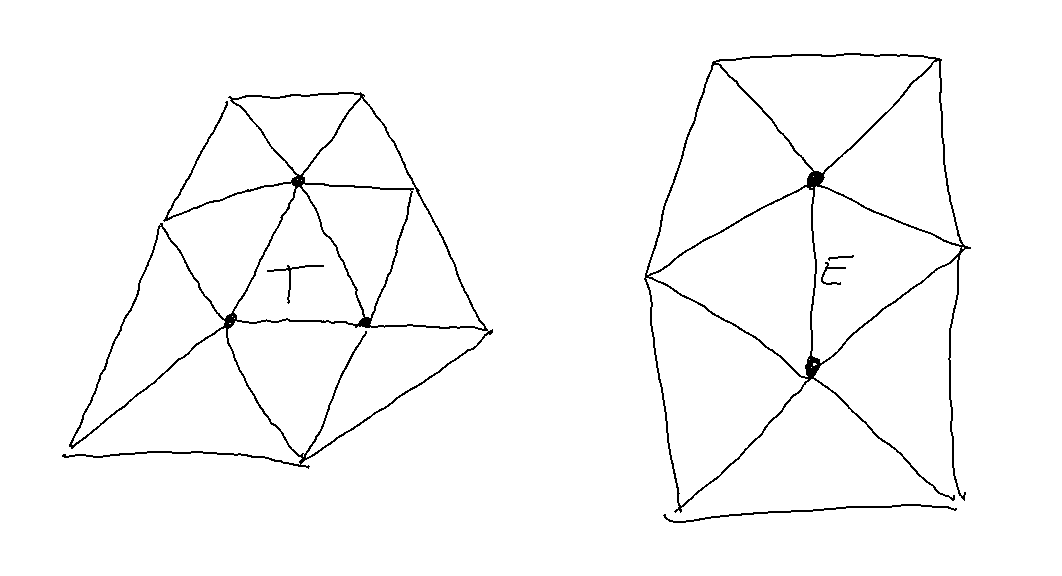
\includegraphics[width=0.75\textwidth]{pics/Sketch9.png}
			\caption{Skizze zur Definition von $\overline{\tilde{\omega}_T}$ (links) und $\overline{\tilde{\omega}_E}$ (rechts)}
			\label{AbbDefinitionUmgebung}
		\end{center}
	\end{figure}
\end{theorem}
% Prof Matthies, nachdem ihm etwas heruntergefallen ist: "Scheiß Schwerkfraft!"

\begin{proof}
	Sei $\mathcal{N}(T)$ die Menge aller Ecken von $T$.
	Sei $\mathcal{N}(E)$ die Menge aller Endpunkte der Kante E. Dann gilt:
	\begin{align*}
		\sum\limits_{z\in\mathcal{N}(T)}\varphi_z|_T=1 \\
		\sum\limits_{z\in\mathcal{N}(E)}\varphi_z|_E=1
	\end{align*}
	\begin{enumerate}[label=\roman*)]
		\item $\begin{aligned}
			\int\limits_{\omega_z}\big(v-\pi_z(v)\big)\d x=0
		\end{aligned}$
		\begin{align*}
			\big\Vert v-\pi_z(v)\big\Vert_{0,2,\omega_z}
			\overset{\ref{korollarPoincareUngleichung}}&\leq
			c_P\cdot\underbrace{\diam(\omega_z)}_{\leq c_3\cdot h_T}\cdot\underbrace{\big|v-\pi_z(v)\big|_{1,2,\omega_z}}_{=|v|_{1,2,\omega_z}}
			=c_4\cdot h_T\cdot|v|_{1,2,\omega_z}
		\end{align*}
		\item
		\begin{align*}
			\big\Vert v-R_h(v)\big\Vert_{0,2,T}=\Bigg\Vert\underbrace{\left(\sum\limits_{z\in\mathcal{N}(T)}\varphi_z\right)}_{=1}\cdot v-\sum\limits_{z\in\mathcal{N}(T)}\pi_z(v)\cdot\varphi_z\Bigg\Vert_{0,2,T}
		\end{align*}
		$T$ hat keine Ecke auf $\partial\Omega=\Gamma$. Also gilt:
		\begin{align*}
			\big\Vert v-R_h(v)\big\Vert_{0,2,T}
			&=\left\Vert\sum\limits_{z\in\mathcal{N}(T)}\big(v-\pi_z(v)\big)\cdot\varphi_z\right\Vert_{0,2,T}\\
			\overset{\text{DU}}&\leq
			\sum\limits_{z\in\mathcal{N}(T)}\Big\Vert\big(v-\pi_z(v)\big)\cdot\underbrace{\varphi_z}_{\in[0,1]}\Big\Vert_{0,2,T}\\
			&\leq
			\sum\limits_{z\in\mathcal{N}(T)}\Big\Vert\big(v-\pi_z(v)\big)\Big\Vert_{0,2,T}\\
			&\leq
			\sum\limits_{z\in\mathcal{N}(T)}\Big\Vert\big(v-\pi_z(v)\big)\Big\Vert_{0,2,\omega_z}\\
			&\leq
			c_4\cdot h_T\cdot\sum\limits_{z\in\mathcal{N}(T)}|v|_{1,2,\omega_z}\\
			&\leq
			3\cdot c_4\cdot h_T\cdot|v|_{1,2,\tilde{\omega}_T}\\
		\end{align*}
		\item $T$ hat mindestens einen Knoten auf $\Gamma$:
		\begin{align*}
			v-R_h(v)
			&=\underbrace{\left(\sum\limits_{z\in\mathcal{N}(T)}\varphi_z\right)}_{=1}\cdot v-\sum\limits_{z\in\mathcal{N}(T)\setminus\Gamma}\pi_z(v)\cdot\varphi_z\\
			&=\sum\limits_{z\in\mathcal{N}(T)}\varphi_z\cdot\big(v-\pi_z(v)\big)+\sum\limits_{z\in\mathcal{N}(T)\cap\Gamma}\big(\pi_z(v)\big)\cdot\varphi_z
		\end{align*}
		Wir berechnen:
		\begin{align*}
			\Big\Vert(\pi_z(v)\big)\cdot\varphi_z\Big\Vert_{0,2,T}
			&\leq
			\big\Vert\underbrace{\pi_z(v)}_{=\text{konst.}}\big\Vert_{0,2,T}
			=\big|\pi_z(v)\big|\cdot|T|^{\frac{1}{2}}
			\leq c_5\cdot h_T\cdot\big|\pi_z(v)\big|
		\end{align*}
		Wenn $z\in\Gamma$, dann ist $E'\subseteq\Gamma$ mit Knoten $z$ und somit:
		\begin{align*}
			\big|\pi_z(v)\big|^2
			&=|E'|^{-1}\cdot\int\limits_{E'}\big|\pi_z(v)\big|^2\d\gamma\\
			&=h_{E'}^{-1}\cdot\big\Vert\pi_z(v)\big\Vert^2_{0,2,E'}\\
			&=h_{E'}^{-1}\cdot\big\Vert\underbrace{v}_{\in H_0^1(\Omega)}-\pi_z(v)\big\Vert^2_{0,2,E'}\\
			&\stackrel{\ref{theoremSkalierterSpursatz}}{\leq}
			c_6^2\cdot h_{E'}^{-1}\cdot\Big(h_{T'}^{-1}\cdot
			\underbrace{\big\Vert v-\pi_z(v)\big\Vert_{0,2,T'}^2}
			_{
			\begin{array}{l}
				\leq\Vert v-\pi_z(v)\Vert^2_{0,2,\omega_z}\\
				\leq c_4^2\cdot h_T^2\cdot|v|^2_{1,2,\omega_z}
			\end{array}}+h_T^{+1}\cdot\underbrace{\big|v-\pi_z(v)\big|^2_{1,2,T'}}_{=|v|^2_{1,2,T'}}\Big)\\
			&\leq
			c_8^2\cdot|v|^2_{1,2,\omega_z} \\
			&\leq
			c_8^2\cdot|v|_{1,2,\tilde{\omega}_T}^2
		\end{align*}
		\begin{align*}
			\implies \Big\Vert\big(\pi_z(v)\big)\cdot\varphi_z\Big\Vert\leq c_9\cdot h_T\cdot|v|_{1,2,\tilde{\omega}_T}
		\end{align*}
		\item  Sei $E$ eine Kante, die keinen Knoten auf $\Gamma$ hat. Dann gilt:
		\begin{align*}
			% the following is not helpful, was just added at the blackboard without use:
			% (in my notes it's in big brackets)
			% \big\Vert v-R_h(v)\big\Vert_{0,2,E}
			% &\leq
			% c\cdot\Big(h_T^{-\frac{1}{2}}\cdot\underbrace{\big\Vert h-R_h(v)\big\Vert_{0,2,T}}_{\leq c\cdot h_T\cdot|v|_{1,2,\tilde{\omega}_T}}+h_T^{\frac{1}{2}}\cdot\underbrace{\big|v-R_h(v)\big|_{1,2,T}}_{=|v|_{1,2,T}}\Big)\\
			\big\Vert v-R_h(v)\big\Vert_{0,2,E}
			&=\Bigg\Vert\sum\limits_{z\in\mathcal{N}(E)}\big(v-\pi_z(v)\big)\cdot\varphi_z\Bigg\Vert_{0,2,E}\\
			&\leq
			\sum\limits_{z\in\mathcal{N}(E)}\big\Vert v-\pi_z(v)\big\Vert_{0,2,E}\\
			&\leq
			c_{10}\cdot\sum\limits_{z\in\mathcal{N}(E)}\Big(h_T^{-\frac{1}{2}}\cdot\underbrace{\big\Vert v-\pi_z(v)\big\Vert_{0,2,T}}_{\leq c\cdot h_T\cdot|v|_{1,2,\omega_z}}+h_T^{\frac{1}{2}}\cdot\underbrace{\big|v-\pi_z(v)\big|_{1,2,T}}_{\leq|v|_{1,2,\omega_z}}\Big)\\
			&\leq
			c\cdot h_E^{\frac{1}{2}}\cdot|v|_{1,2,\tilde{\omega}_E}
		\end{align*}
		\item $E$ hat hat einen Knoten auf dem Rand $Γ$. %Knotenbeschränkung
			Diesen Fall lassen wir hier aus.
			% ist das richtig? Auf jeden Fall sehe ich weder hier noch in meinen Notizen einen Hinweis auf diesen Fall.
		\begin{align*}
			R(v)&=l(v)-a(u_h,v)=l(v-v_h)-a(u_h,v-v_h)\qquad\forall v_h\in X_h\\
			&\leq\sum\limits_{T\in\T_h}\big\Vert f+\Delta u_h\big\Vert_{0,2,T}\cdot\Vert v-v_h\Vert_{0,2,T}\\
			&{}\quad+\sum\limits_{E\in\Sigma_h}\big\Vert[\nabla u_h\cdot n_E]_E\big\Vert_{0,2,E}\cdot\Vert v-v_h\Vert_{0,2,E}
		\end{align*}
		Idee: Nutze $v_h=R_h(v)$.
		\begin{align*}
			R(v)&\leq
			c\cdot\sum\limits_{T\in\T_h}\Big(\left\Vert f+ \Delta u_h\big\Vert_{0,2,T}\cdot h_T\right)\cdot |v|_{1,2,\tilde{\omega}_T}\\
			&\quad+c\cdot\sum\limits_{E\in\Sigma_h}\left(\Big\Vert[\nabla u_h\cdot n_E]_E\Big\Vert_{0,2,E}\cdot h_E^{\frac{1}{2}}\right)\cdot|v|_{1,2,\tilde{\omega}_E}\\
			&\leq
			c\cdot\left(\sum\limits_{T\in\T_h}\big\Vert f+\Delta u_h\big\Vert^2_{0,2,T}\cdot h_T^2\right)^{\frac{1}{2}}\cdot\left(\sum\limits_{T\in\T_h}|v|^2_{1,2,\tilde{\omega}_T}\right)^{\frac{1}{2}}\\
			&\quad+c\cdot\left(\sum\limits_{E\in\Sigma_h}\big\Vert[\nabla u_h\cdot n_E]_E\big\Vert^2_{0,2,E}\cdot h_E\right)\cdot\underbrace{\left(\sum\limits_{E\in\Sigma_h}|v|^2_{1,2,\tilde{\omega}_E}\right)^{\frac{1}{2}}}_{\leq c\cdot |v|_{1,2,\Omega}\text{, $c$ aus Formregulärität}}\\
			&\leq
			c\cdot\underbrace{\left(\sum\limits_{T\in\T_h} h^2_T\cdot\big\Vert f+\Delta u_h\big\Vert^2_{0,2,T}
			+\sum\limits_{E\in\Sigma_h}h_E\cdot\big\Vert[\nabla u_h\cdot n_E]_E\big\Vert^2_{0,2,E}\right)^{\frac{1}{2}}}_{:=\eta}\cdot\Vert v\Vert_{1,2,\Omega}\nl
			&\implies
			\Vert u-u_h\Vert_{1,2,\Omega}
			\leq
			c\cdot\sup\limits_{\begin{subarray}{c}v\in H_0^1(\Omega)\\\Vert v\Vert_{1,2,\Omega}=1\end{subarray}}R(v) \leq c \cdot \eta
		\end{align*}
		Setze
		\begin{align*}
			\eta_T^2&:=h_T^2\cdot\big\Vert f+\Delta u_h\big\Vert^2_{0,2,T}+\frac{1}{2}\cdot\sum\limits_{E\in\Sigma_k\cap\partial T}h_E\cdot\big\Vert[\nabla u_h\cdot n_E]_E\big\Vert^2_{0,2,E}\\
			\eta:&=\left(\sum\limits_{T\in\T_h}\eta^2_T\right)^{\frac{1}{	2}}
		\end{align*}
		$\eta$ ist eine zuverlässige a posteriori Fehler-Abschätzung. \qedhere
	\end{enumerate}
\end{proof}

\begin{definition}[Bubble-Funktion]\enter %no number, but i will give some
	Sei $T\in\T_h$ und $E\in\Sigma_h$. Wir setzen
	\begin{align*}
		\psi_T:=27\cdot\varphi_{z_1}\cdot\varphi_{z_2}\cdot\varphi_{z_3}
	\end{align*}
	wobei $z_1,z_2,z_3$ die Ecken von $T$ sind. Definiere weiterhin
	\begin{align*}
		\psi_E:=4\cdot\varphi_{z_1}\cdot\varphi_{z_2}
	\end{align*}
	wobei $z_1,z_2$ die Enden der Kante $E$ sind.
\end{definition}

\begin{lemma}[Eigenschaften]\ %no lemma in lecture
	\begin{enumerate}[label=\roman*)]
		\item $\begin{aligned}
			\psi_T\in P_3(T)
			\hspace{64pt}
			\psi_E\big|_T\in P_2(T)\qquad\forall\, T\in\omega_E
		\end{aligned}$
		\item $\begin{aligned}
			\psi_T\geq0\text{ in }\overline{T}
			\hspace{61pt}
			\psi_E\geq 0\text{ in }\overline{\omega}_E
		\end{aligned}$
		\item $\begin{aligned}
			\psi_T\equiv0\text{ auf }\partial T
			\hspace{50pt}
			\psi_E\equiv 0\text{ auf }\partial\omega_E
		\end{aligned}$
		\item $\begin{aligned}
			\max\limits_{x\in\overline{T}}\psi_T(x)=1
			\hspace{48pt}
			\max\limits_{x\in\overline{\omega}_E}\psi_E(x)=1
		\end{aligned}$
		\item $\begin{aligned}
			\hspace{120pt}
			\psi_E\in C(\omega_E)
		\end{aligned}$
	\end{enumerate}
\end{lemma}

\begin{theorem}
	Sei $T\in\T_h,E\in\Sigma_h, v\in P_k(T), \sigma\in P_k(E)$. Dann gilt:
	% todo: wäre es nicht sinnvoller align zu nutzen und damit die Nummerierung aus align zu nutzen und jede Zeile mit einem Label zu versehen? Sieht auf jeden Fall besser aus, da keine Leerzeigen dabei sind
	\begin{enumerate}[label=(\arabic*)]
		\item
		\begin{align*}
			c_1\cdot\Vert v\Vert_{0,2,T}
			\leq\left(\int\limits_T\psi_T\cdot v^2(x)\d x\right)^{\frac{1}{2}} \leq\Vert v\Vert_{0,2,T}
		\end{align*}
		\item
		\begin{align*}
			c_2\cdot h_T^{-1}\cdot\big\Vert\psi_T v\big\Vert_{0,2,T}\leq\big|\psi_T v\big|_{1,2,T}\leq c_3\cdot h_T^{-1}\cdot\big\Vert\psi_T v\big\Vert_{0,2,T}
		\end{align*}
		\item
		\begin{align*}
			c_4\cdot\Vert\sigma\Vert_{0,2,E} \leq\left(\int\limits_E\psi_E\cdot\sigma^2\d s\right)^{\frac{1}{2}}\leq \Vert\sigma\Vert_{0,2,E}
		\end{align*}
		\item
		\begin{align*}
			c_5\cdot h_E^{-1}\cdot\big\Vert\psi_E\sigma\big\Vert_{0,2,\omega_E}
			\leq\big|\psi_E\sigma\big|_{1,2,\omega_E}
			\leq c_6\cdot h_E^{-1}\cdot\big\Vert\psi_E\sigma\big\Vert_{0,2,\omega_E}
		\end{align*}
		\item
		\begin{align*}
			\big\Vert\psi_E\sigma\big\Vert_{0,2,\omega_E}
			\leq c_7\cdot h_E^{\frac{1}{2}}\cdot\Vert\sigma\Vert_{0,2,E}
		\end{align*}
	\end{enumerate}
\end{theorem}
\begin{proof}
	Beweisskizze: Es sollte sich alles durch Transformation zum Referenzelement ergeben. Dann Normäquivalenz auf dem endlich dimensionalem Raum.
\end{proof}

$f_h$ ist eine stückweise  polynomielle Approximation von $f$, z.B.
\begin{align*}
	f_h\big|_T:=L^2\text{-Projektion von $f$ auf }P_h(T)
\end{align*}

\begin{align*}
	c^2_1\cdot\big\Vert f_h+\Delta u_h\big\Vert^2_{0,2,T}
	&\leq\int\limits_T\big(f_h+\Delta u_h\big)\cdot\underbrace{\big(f_h+\Delta u_h\big)\cdot\psi_T}_{=:v_T\in H^1_0(\Omega)\mit v_T|_{\partial T}=0}\d x\\
	&=\int\limits_T\big(f+\Delta u_h\big)\cdot v_T\d x+\int\limits_T\big(f_h-f\big)\cdot v_T\d x\\
	&\quad+\int\limits_{\partial T}\nabla u_h\cdot n_T\cdot\underbrace{v_T}_{=0}\d\gamma\\
	\overset{\text{part Int}}&=
	\int\limits_T\big(\nabla u-\nabla u_h\big)\cdot\nabla v_T\d x+\int\limits_T\big(f_h-f\big)\cdot v_T\d x\\
	\overset{\text{CS}}&\leq
	\big\Vert u-u_h\big\Vert_{1,2,T}\cdot\halfnorm{v_T}_{1,2,T}+\big\Vert f-f_h\big\Vert_{0,2,T}\cdot\big\Vert v_T\big\Vert_{0,2,T}\\
	&\leq
	c_3\cdot h_T^{-1}\cdot\big\Vert u-u_h\big\Vert_{1,2,T}\cdot\big\Vert\overbrace{v_T}^{\mathclap{=\psi_T\big(f_h+\Delta u_h\big)}}\big\Vert_{0,2,T}\\
	&\quad+\big\Vert f-f_h\big\Vert_{0,2,T}\cdot\big\Vert v_T\big\Vert_{0,2,T}\\
	&\leq
	c\cdot h^{-1}_T\cdot\big\Vert u-u_h\big\Vert_{1,2,T}\cdot\big\Vert f_h+\Delta u_h\big\Vert_{0,2,T}\\
	&\quad+\big\Vert f-f_h\big\Vert_{0,2,T}\cdot\big\Vert f_h+\Delta u_h\big\Vert_{0,2,T}
\end{align*}
Hierbei wird auch benutzt:
\begin{align*}
	\int\limits_T f\cdot v_T\d x=\int\limits_\Omega f\cdot v_T\d x=\int\limits_\Omega \nabla u\cdot\nabla v_T\d x=\int\limits_T\nabla u\cdot\nabla v_T\d x
\end{align*}
Multiplikation mit $\frac{h_T}{\Vert f_h+\Delta u_h\Vert_{0,2,T}}$ liefert:
\begin{align*}
	c_1^2\cdot h^T\cdot\big\Vert f_h+\Delta u_h\big\Vert_{0,2,T}
	&\leq c\cdot\big\Vert u-u_h\big\Vert_{1,2,T}+h_T\cdot\big\Vert f-f_h\big\Vert_{0,2,T}\\
\end{align*}
Und so erhalten wir:
\begin{align*}
	h_T\cdot\big\Vert f+\Delta u_h\big\Vert_{0,2,T}
	&\leq h_T\cdot\big\Vert f_h+\Delta u_h\big\Vert_{0,2,T}+h_T\cdot\big\Vert f-f_h\big\Vert_{0,2,T}\\
	&\leq c\cdot\big\Vert u-u_h\big\Vert_{1,2,T}+c\cdot h_T\cdot\big\Vert f-f_h\big\Vert_{0,2,T}
\end{align*}
\begin{align*}
	c_4^2\cdot\big\Vert[\nabla u_h\cdot n_E]_E\big\Vert^2_{0,2,E}
	&=\int\limits_E\big[\nabla u_h\cdot n_E\big]_E\cdot\underbrace{\big[\nabla u_h\cdot n_E\big]_E\cdot\psi_E}_{=:v_E\in H^1_0(\omega_E)\subseteq H_0^1(\Omega)} \d γ\\
	&=\int\limits_E\big[\nabla u_h\cdot n_E\big]_E\cdot v_E\d\gamma+\int\limits_{\omega_E}\big(f+\Delta u_h\big)\cdot v_E\d x\\
	&\quad-\int\limits_{\omega_E}\big(f+\Delta u_h\big)\cdot v_E\d x\\
	\overset{\substack{\text{part Int +}\\\text{schwache Form.}}}&=
	a\big(u-u_h,v_E\big)-\sum\limits_{T\in\omega_E}\int\limits_T\big(f+\Delta u_h\big)\cdot v_E\d x\\
	&\leq
	\big\Vert u-u_h\big\Vert_{1,2,\omega_E}\cdot\big|v_E\big|_{1,2,\omega_E}\\
	&\quad+\left(\sum\limits_{T\in\omega_E}\big\Vert f+\Delta u_h\big\Vert^2_{0,2,T}\right)^{\frac{1}{2}}\cdot\big\Vert v_E\big\Vert_{0,2,\omega_E}\\
	&\leq
	\big\Vert u-u_h\big\Vert_{1,2,\omega_E}\cdot c_6\cdot c_7\cdot h_E^{-\frac{1}{2}}\cdot\big\Vert[\nabla u_h\cdot n_E]_E\big\Vert_{0,2,E}\\
	&\quad + c_7\cdot h_E^{\frac{1}{2}}\cdot\left(\sum\limits_{T\in\omega_E}\big\Vert f+\Delta u_h\big\Vert^2_{0,2,T}\right)^{\frac{1}{2}}\cdot\big\Vert[\nabla u_h\cdot n_E]_E\big\Vert_{0,2,E}
\end{align*}
\begin{align*}
	\implies &h_E^{\frac{1}{2}}\cdot\big\Vert[\nabla u_h\cdot n_E]_E\big\Vert_{0,2,E} \\
	\leq &c_8\cdot\Bigg(\big\Vert u-u_h\big\Vert_{1,2,\omega_E}+\bigg(\underbrace{\sum\limits_{T\in\omega_E} h^2_T\cdot\big\Vert f+\Delta u_h\big\Vert^2_{0,2,T}}_{\leq c\cdot\Vert u-u_h\Vert_{1,2,\omega_E}+h_E\cdot\Vert f-f_h\Vert_{0,2,\omega_E}}\bigg)^{\frac{1}{2}}\Bigg)
\end{align*}
Also
\begin{align*}
	\eta_T&\leq c\cdot\big\Vert u-u_h\big\Vert_{1,2,\omega_T}+c\cdot h_T\cdot\big\Vert f-f_h\big\Vert_{0,2,\omega_T}\\
	&\implies\eta_T\text{ ist effizient}
\end{align*}

\subsection{Algorithmus (adaptive Gitterverfeinerung)}
\texttt{
\begin{enumerate}[start=0]
	\item Wähle eine Start-Triangulierung $\mathcal{T}_0$, Setze $l:=0$
	\item Löse das diskrete Problem auf $\mathcal{T}_l$
	\item Berechne $\eta_T$, $T\in\T_l$
	\begin{align*}
		\eta_l:=\max\limits_{T\in\T_l}\eta_T,\qquad\eta:=\left(\sum\limits_{T\in\mathcal{T}_l}\eta_T^2\right)^{\frac{1}{2}}
	\end{align*}
	\item Falls $\eta_l\leq\varepsilon$ STOP
	\item Verfeinere alle Zellen $T$ mit $\eta_T\geq\gamma \cdot \eta_l$\\
	Verfeinere andere Dreiecke um die Regularität des Gitters\\ sicherzustellen
	\begin{align*}
		l:=l+1,\qquad\texttt{GOTO }1
	\end{align*}
\end{enumerate}}
Die Wahl von $\gamma\in[0,1]$:\\
$\gamma$ klein $\rightsquigarrow$ Verfeinerung von vielen Dreiecken\\
$\gamma$ groß $\rightsquigarrow$ Verfeinerung von wenigen Dreiecken

\subsection{Verfeinerungs-Pattern von Dreiecken} %noNumber
Wenn wir bei hängenden Knoten die benachbarten Dreiecke nach dem normalen Schema verfeinern, stoßen wir auf ungewollte Probleme.
Zwangsweise wird dadurch das komplette Gebiet verfeinert.

\begin{figure}[!ht]
	\begin{center}
		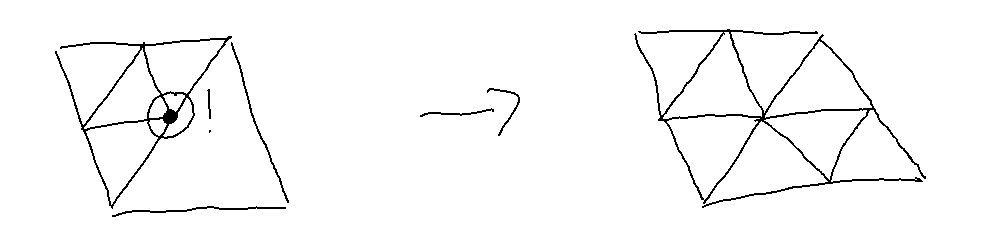
\includegraphics[width=\textwidth]{pics/Sketch10.png}
		\caption{Unnötig starke Verfeinerung um hängenden Knoten zu beheben}
		\label{AbbVerfeinerung}
	\end{center}
\end{figure}

Deshalb führen wir folgende Typen von Verfeinerungen ein:
\begin{itemize}
	\item \color{red}rote Verfeinerung\color{black}: normale Verfeinerung: Unterteile ein Dreick in 4 Teildreicke
	\item \color{green}grüne Verfeinerung\color{black}: verbinde den Mittelpunkt der \ul{längsten} Kante mit der entgegengesetzten Ecke
	\item \color{blue}blaue Verfeinerung\color{black}: Verbinde den Mittelpunkt der \underline{längsten} Kante mit der entgegengesetzten Ecke und mit einem Mittelpunkt einer anderen Kante
\end{itemize}

\begin{figure}[H]
	\center
	\begin{tikzpicture}[scale=1]
	\def \xone{0};
	\def \yone{0};
	\def \h{3};
	
	% first triangle   red
	\coordinate (A) at (\xone,\yone);
	\coordinate (B) at ($ (A) + (1.4*\h,0) $);
	\coordinate (C) at ($ (A) + (0.7*\h,0.7*\h) $);
	\coordinate (AB) at ($ (A) + (0.7*\h,0) $);
	\coordinate (AC) at ($ (A) + (0.35*\h,0.35*\h) $);
	\coordinate (BC) at ($ (A) + (1.05*\h,0.35*\h) $);

	%draw		
	\draw (A) -- (B) -- (C) --cycle;
	\draw[red] (AB) -- (AC) -- (BC) --cycle;
	\foreach \i in {A,B,C,AB,AC,BC}{
		\filldraw (\i) circle (1.5pt);
	}

	% second triangle   green
	\coordinate (A1) at (\xone + 1.6*\h,\yone);
	\coordinate (B1) at ($ (A1) + (1.4*\h,0) $);
	\coordinate (C1) at ($ (A1) + (0.7*\h,0.7*\h) $);
	\coordinate (AB1) at ($ (A1) + (0.7*\h,0) $);

	%draw			
	\draw (A1) -- (B1) -- (C1) --cycle;
	\draw[green] (AB1) -- (C1);
	\foreach \i in {A1,B1,C1,AB1}{
		\filldraw (\i) circle (1.5pt);
	}

	% third triangle   blue
	\coordinate (A2) at (\xone + 0.8*\h,\yone - \h);
	\coordinate (B2) at ($ (A2) + (1.4*\h,0) $);
	\coordinate (C2) at ($ (A2) + (0.7*\h,0.7*\h) $);
	\coordinate (AB2) at ($ (A2) + (0.7*\h,0) $);
	\coordinate (BC2) at ($ (A2) + (1.05*\h,0.35*\h) $);

	%draw			
	\draw (A2) -- (B2) -- (C2) --cycle;
	\draw[blue] (AB2) -- (C2);
	\draw[blue] (AB2) -- (BC2);
	\foreach \i in {A2,B2,C2,AB2}{
		\filldraw (\i) circle (1.5pt);
	}
\end{tikzpicture}
	\caption{Verfeinerung: rot,grün,blau}
	\label{AbbRefinement_types}
\end{figure}

\textbf{Schritt 4:}
\begin{enumerate}[label=\alph*)]
	\item $\eta_T\geq\gamma\cdot\eta_l\implies\text{ rote Verfeinerung}$
	\item drei hängende Knoten $\implies$ rote Verfeinerung
	\begin{figure}[!ht]
		\begin{center}
			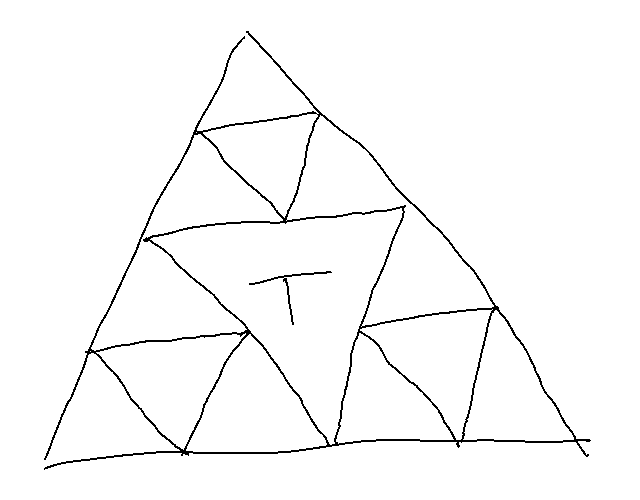
\includegraphics[width=0.4\textwidth]{pics/Sketch11.png}
			\caption{Fall b}
			\label{AbbVerfeinerungB}
		\end{center}
	\end{figure}
	\item zwei hängende Knoten, beide \underline{nicht} auf der längsten Kante $\implies$ rote Verfeinerung
	\begin{figure}[!ht]
		\begin{center}
			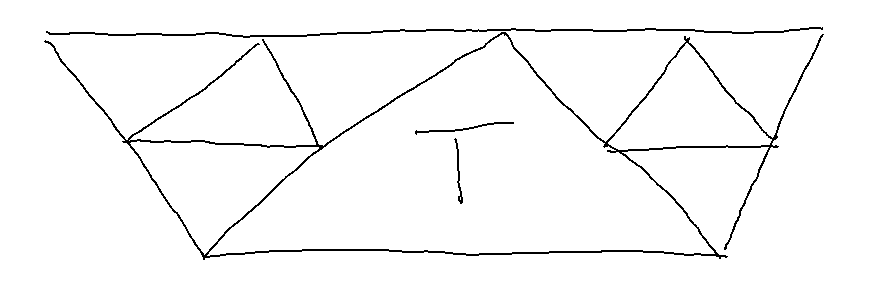
\includegraphics[width=0.4\textwidth]{pics/Sketch12.png}
			\caption{Fall c}
			\label{AbbVerfeinerungC}
		\end{center}
	\end{figure}
	\item zwei hängende Knoten, eine auf der längsten Kante $\implies$ blaue Verfeinerung
	\begin{figure}[!ht]
		\begin{center}
			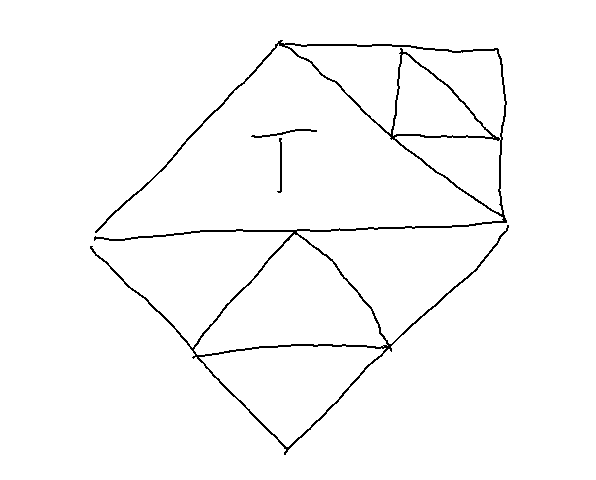
\includegraphics[width=0.4\textwidth]{pics/Sketch13.png}
			\caption{Fall d}
			\label{AbbVerfeinerungD}
		\end{center}
	\end{figure}
	\item ein hängender Knoten, \underline{nicht} auf der längsten Kante $\implies$ blaue Verfeinerung
	\begin{figure}[!ht]
		\begin{center}
			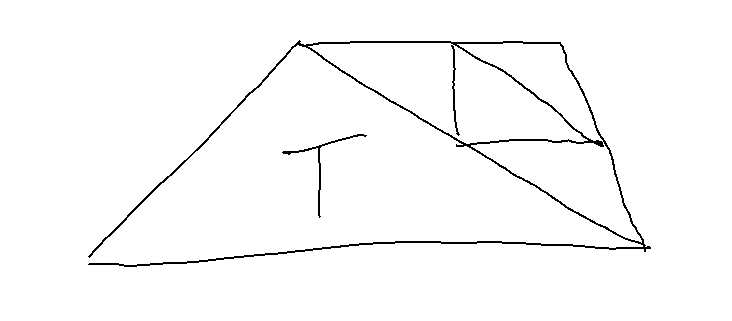
\includegraphics[width=0.4\textwidth]{pics/Sketch14.png}
			\caption{Fall e}
			\label{AbbVerfeinerungE}
		\end{center}
	\end{figure}
	\item ein hängender Knoten auf der längsten Kante $\implies$ grüne Verfeinerung
	\begin{figure}[!ht]
		\begin{center}
			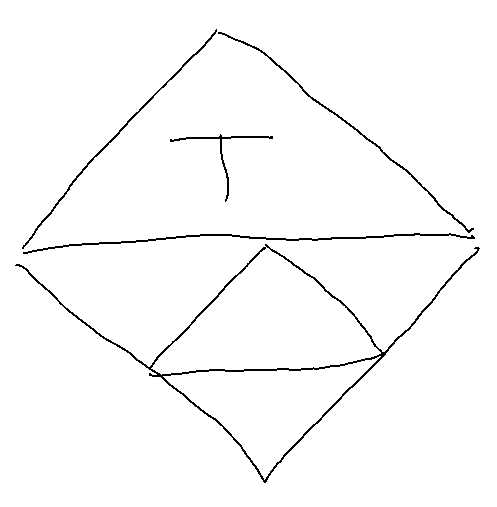
\includegraphics[width=0.3\textwidth]{pics/Sketch15.png}
			\caption{Fall f}
			\label{AbbVerfeinerungF}
		\end{center}
	\end{figure}
\end{enumerate}
	% This work is licensed under the Creative Commons
% Attribution-NonCommercial-ShareAlike 4.0 International License. To view a copy
% of this license, visit http://creativecommons.org/licenses/by-nc-sa/4.0/ or
% send a letter to Creative Commons, PO Box 1866, Mountain View, CA 94042, USA.
% vim: set noexpandtab:

\section{Stromlinien-Diffusions-Methode (SDFEM)} %7.
Hughes / Brooks 1979

\subsection{Motivation}
\begin{align*}
\left\lbrace
	\begin{array}{rl}
	-\varepsilon\cdot\Delta u+b\cdot \nabla u+c\cdot u=f&\text{ in }\Omega\\
	u=g&\text{ auf }\Gamma=\partial\Omega\\
	0<\varepsilon\ll 1&
	\end{array}
	\right.
\end{align*}

Für $\varepsilon=0$ ist dies eine PDE erster Ordnung, aber für $\varepsilon>0$ eine PDE zweiter Ordnung.
Beim Grenzübergang passieren "magische Dinge", die sich mit den bisher bekannten Verfahren nicht sinnvoll lösen lassen.
Es kommt zu Oszillationen.
Deshalb wurden die SDFEM-Verfahren erfunden.
Die Idee besteht darin aus das diskrete Problem noch $\delta_K$-mal das glatte Problem dazu zu addieren.\nl
\textbf{1D:}
\begin{align*}
	-\varepsilon\cdot u''+u'=0\text{ auf }(0,1),\qquad u(0)=0,\qquad u(1)=1
\end{align*}
\begin{figure}[!ht]
	\begin{center}
		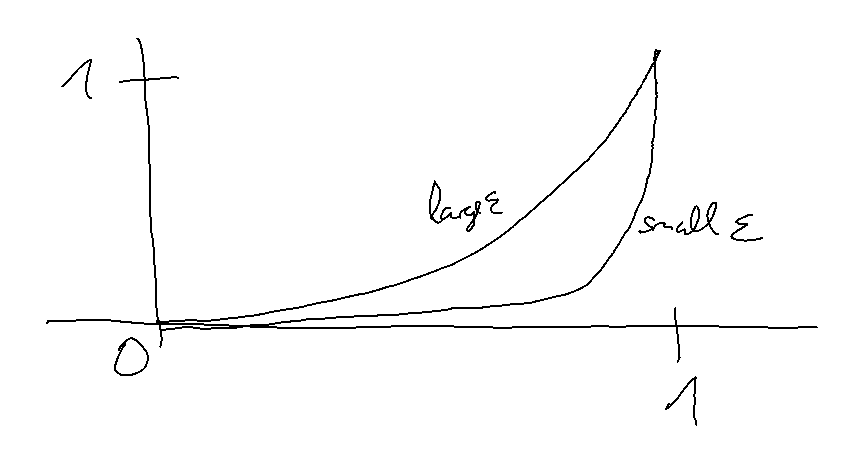
\includegraphics[width=0.7\textwidth]{pics/Sketch16.png}
		\caption{Skizze für kleines und großes $\epsilon$}
		\label{AbbEinfachesStromlinienProblem}
	\end{center}
\end{figure}

ersetze $\varepsilon$ durch Gitterparameter $h$.\\
$\implies$ keine Oszillation, aber "Verschmierung" %smearing

Verschmierung hauptsächlich in Seitenwindrichtung
$b$ und $b^\perp$ sind orthogonale Einheitsvektoren
\begin{align*}
	\Delta u&=\frac{\partial^2 u}{\partial x^2}+\frac{\partial^2 u}{\partial y^2}
	=\frac{\partial^2 u}{\partial b^2}+\frac{\partial^2 u}{\partial (b^T)^2}\\
	\varepsilon\cdot\Delta u&\to\varepsilon\cdot\frac{\partial^2 u}{\partial(b^T)^2}+h\cdot\frac{\partial^2 u}{\partial b^2}
\end{align*}
Hier nur Konvergenz erster Ordnung in $h$.

\subsection{SDFEM Diskretisierung}
\textbf{Modellproblem}
\begin{align}\label{eq7.2_1}\tag{1}
	\left\lbrace\begin{array}{rl}
		-\varepsilon\Delta u+b\cdot\nabla u+cu&=f\text{ in }\Omega\\
		u&=0\text{ auf }\Gamma=\partial\Omega
	\end{array}\right.
\end{align}
Diskretisierung: stetige $P_r$-Elemente $\to V_h\subseteq H_0^1(\Omega)$\\
$u\in H^2(\Omega)$, $b,c$ hinreichend glatt
\begin{align}\nonumber
	-\varepsilon\Delta u+b\cdot \nabla u+cu&= f&&\text{ im }L^2\text{- Sinn}\\
	\implies\Big(-\varepsilon\Delta u+b\cdot\nabla u+cu,b\cdot\nabla v_h\Big)_K&=\big(f,b\cdot\nabla v_h\big)_K
	&&\forall K\in\T_h,v_h\in V_h
	\label{eq7.2_2}\tag{2}
\end{align}

mit
\begin{align*}
	(\varphi,\psi):&=\int\limits_K\varphi(x)\cdot\psi(x)\d x
\end{align*}
Zusätzlich: (Einschränkung auf schwache Formulierung von $V_h$):
\begin{align*}\label{eq7.2_3}\tag{3}
	\varepsilon(\nabla u,\nabla v)+(b\cdot\nabla u+ cu,v_h)=(f,v_h)\qquad\forall v_h\in V_h
\end{align*}
$(\cdot,\cdot)=(\cdot,\cdot)_\Omega$\nl
$u$ erfüllt:
\begin{align}\label{eq7.2_4}\tag{4}
	a_h(u,v_h)&=f_h(v_h)\qquad\forall v_h\in V_h
\end{align}
wobei
\begin{align}\label{eq7.2_5}\tag{5}
	a_h(u,v)&:=\varepsilon(\nabla u,\nabla v)+(b\cdot\nabla u+cu, v)\\\nonumber
	&\qquad+\sum\limits_{K\in\T_h}\delta_K\Big(-\varepsilon\Delta u+b\cdot\nabla u+cu,b\cdot\nabla v\Big)_K\\
	\label{eq7.2_6}\tag{6}
	f_h(v_h)&:=(f,v_h)+\sum\limits_{K\in\T_h}\delta_K(f,b\cdot\nabla v)_K
\end{align}

\textbf{Idee:} Diskretes Problem:\\
Finde $u_h\in V_h$ so, dass
\begin{align}\label{eq7.2_7}\tag{7}
	a_h(u_h,v_h)&=f_h(v_h)\qquad\forall v_h\in V_h
\end{align}
Damit folgt aus \eqref{eq7.2_4} und \eqref{eq7.2_7}:
\begin{align}\label{eq7.2_8}\tag{8}
	a_h(u-u_h,v_h)=0\qquad\forall v_h\in V_h
\end{align}
Also die Galerkin Orthogonalität.\nl
\textbf{Wahl von $\delta_k$:}\\
Die \textbf{lokale Peclét-Zahl} ist
\begin{align*}
	p_{e_K}:=\frac{\Vert b\Vert_{0,\infty,K}}{2\cdot\varepsilon}\cdot h_K
\end{align*}
Hängt mit der Beziehung zwischen Konvention und Diffusion zusammen.
\begin{align}\label{eq7.2_9}\tag{9}
	\delta_K:=\left\lbrace\begin{array}{cl}
		\delta_0 h_K, &\falls p_{e_K}>1\\
		\frac{\delta_1 h_K^2}{\varepsilon}, &\falls p_{e_K}\leq 1
	\end{array}\right.
\end{align}
Hierbei sind $\delta_0,\delta_1$ Konstanten.\nl
\textbf{Spezialfall: 2D, stetige $P_1$-Elemente, $c\equiv0$, $b\equiv(b_1,b_2)=$ konstant}\\
Also erhält man
\begin{align*}
	a_h(u_h,v_h)&=\varepsilon\big(\nabla u_h,\nabla v_h\big)+(b\cdot\nabla u_h,v_h)
	+\underbrace{\sum\limits_{K\in\T_h}\delta_K\big(b\cdot\nabla u_h,b\cdot\nabla v_h\big)_K}_{\text{zusätzliche Diffsion in Richtung }b}
\end{align*}

\subsection{Konvergenzanalysis}
Annahmen:
\begin{itemize}
	\item $b,c,f$ seien hinreichend glatt
	\item für die eindeutige Lösbarkeit nehmen wir an
	\begin{align}\label{eq7.3_10}\tag{10}
		c-\frac{1}{2}\div(b)\geq0\text{ in }\Omega
	\end{align}
	\item $V_h$: stetige $P_r$-Elemente, $V_h\subseteq H_0^1(\Omega)$
	\item Lokalinversen-Ungleichung
	\begin{align}\label{eq7.3_11}\tag{11}
		\Vert\Delta v_h\Vert_{0,2,K}\leq\mu_{\text{inv}}\cdot h^{-1}_K\cdot|v_h|_{1,2,K}
		\qquad\forall v_h\in V_h,\forall K\in\T_h
	\end{align}
	$\mu_{\text{inv}}$ ist unabhängig von $K$
	\item SD-Norm
	\begin{align}\label{eq7.3_12}\tag{12}
		\Vert v\Vert_{\text{SD}}:=\left(\varepsilon|v|_{1,2,\Omega}^2+c_0\Vert v\Vert_{0,2,\Omega}^2+\sum\limits_{K\in\T_h}\delta_K\Vert b\cdot\nabla v\Vert^2_{0,2,K}\right)^{\frac{1}{2}}
	\end{align}
\end{itemize}

\begin{lemma}[Koerzivität]\label{lemma7.1Koerzivitaet}
	Sei
	\begin{align*}
		c_k:=\Vert c\Vert_{0,\infty,\Omega}=\max\limits_{x\in K}\big|c(x)\big|>0
	\end{align*}
	und
	\begin{align}\label{eq7.3_13}\tag{13}
		0<\delta_K\leq\frac{1}{2}\cdot\min\left\lbrace\frac{c_0}{c_K^2},\frac{h_K^2}{\varepsilon\cdot\mu_{\text{inv}}^2}\right\rbrace
	\end{align}
	Dann ist $a_h$ koerziv im folgenden Sinn:
	\begin{align}\label{eq7.3_14}\tag{14}
		a_h(v_h,v_h)\geq\frac{1}{2}\cdot\Vert v_h\Vert_{\text{SD}}^2\qquad\forall v_h\in V_h
	\end{align}
\end{lemma}

\begin{proof}
	Erinnerung:
	\begin{align*}
		\big(b\cdot\nabla v_h,v_h\big)&=\frac{1}{2}\cdot\big(\div(b)\cdot v_h^2\big)
	\end{align*}
	Damit also:
	\begin{align*}
		\implies a_h(v_h,v_h)
		&=\varepsilon(\nabla v_h,\nabla v_h)+(b\cdot\nabla v_h,v_h)+(c \cdot v_h,v_h)\\
		&~+\sum\limits_{K\in\T_h}\delta_K\Big(-\varepsilon\Delta v_h+b\cdot\nabla v_h+c \cdot v_h,b\cdot\nabla v_h\Big)_K\\
		&=\varepsilon|v_h|^2_{1,2,\Omega}+\Big(\underbrace{c-\frac{1}{2}\cdot\div(b)}_{\geq c_0>0},v_h^2\Big)+\sum\limits_{K\in\T_h}\delta_K\big(b\cdot\nabla v_h,b\cdot \nabla v_h\big)_K\\
		&~+\underbrace{\sum\limits_{K\in\T_h}\delta_K\big(-\varepsilon\Delta v_h,b\cdot\nabla v_h\big)_K}_{=:T_1}
		+\underbrace{\sum\limits_{K\in\T_h}\delta_K\big(c \cdot v_h,b\cdot\nabla v_h\big)_K}_{=:T_2}\\
		&\geq\underbrace{\varepsilon|v_h|^2_{1,2,\Omega}+c_0\Vert v_h\Vert^2_{0,2,\Omega}+\sum\limits_{K\in\T_h}\delta_K\Vert b\cdot\nabla v_h\Vert^2_{0,2,K}}_{=\Vert v\Vert^2_{\text{SD}}}-|T_1|-|T_2|
	\end{align*}
	Jetzt müssen wir noch $T_1$ und $T_2$ abschätzen.
	\begin{align*}
		|T_1|
		&\leq\sum\limits_{K\in\T_h}\delta_K\varepsilon\Big|(\Delta v_h,b\cdot\nabla v_h)_K\Big| \\
		&\overset{\text{CS}}{\leq}
		\sum\limits_{K\in\T_h}\delta_K\varepsilon\Vert\Delta v_h\Vert_{0,2,K}\cdot\Vert b\cdot\nabla v_h\Vert_{0,2,K}\\
	\end{align*}
	Mit
	\begin{align*}
		\alpha\beta
		&\leq\alpha^2+\frac{1}{4}\beta^2\\
		\alpha&=\varepsilon\delta_K^{\frac{1}{2}}\Vert\Delta v_h\Vert_{0,2,K}\\
		\beta&=\delta_K^{\frac{1}{2}}\Vert b\cdot\nabla v_h\Vert_{0,2,K}
	\end{align*}
	gilt
	\begin{align*}
		&\sum\limits_{K\in\T_h}\delta_K\varepsilon\Vert\Delta v_h\Vert_{0,2,K}\cdot\Vert b\cdot\nabla v_h\Vert_{0,2,K} \\
		&\leq
		\sum\limits_{K\in\T_h}\underbrace{\varepsilon^2\delta_K\underbrace{\Vert\Delta v_h\Vert^2_{0,2,K}}_{\overset{\eqref{eq7.3_11}}{\leq}\mu^2_{\text{inv}} h_K^{-1}|v_h|^2_{1,2,K}}}_{\leq\underbrace{\varepsilon^2\delta_K\mu^2_{\text{inv}} h_K^{-2}}_{\overset{\eqref{eq7.3_13}}{\leq}\frac{\varepsilon}{2}}|v_h|^2_{1,2,K}}\\
		&\leq\frac{1}{2}\varepsilon|v_h|^2_{1,2,\Omega}+\frac{1}{4}\sum\limits_{K\in\T_h}\delta_K\Vert b\cdot\nabla v_h\Vert^2_{0,2,K}
	\end{align*}
	Für $T_2$ erhalten wir die Abschätzung
	\begin{align*}
		|T_2|
		&\leq\sum\limits_{K\in\T_h}\delta_K\Big|(c \cdot v_h,b\cdot\nabla v_h)_K\Big|\\
		&\leq\sum\limits_{K\in\T_h}\delta_K c_K\Vert v_h\Vert_{0,2,K}\Vert b\cdot\nabla v_h\Vert_{0,2,K}
	\end{align*}
	Mit
	\begin{align*}
		\alpha&=\delta_K^{\frac{1}{2}}c_K\Vert v_h\Vert_{0,2,K}\\
		\beta&=\delta_K^{\frac{1}{2}}\Vert b\cdot\nabla v_h\Vert_{0,2,K}
	\end{align*}
	gilt
	\begin{align*}
		&\sum\limits_{K\in\T_h}\delta_K c_K\Vert v_h\Vert_{0,2,K}\Vert b\cdot\nabla v_h\Vert_{0,2,K} \\
		&\leq\sum\limits_{K\in\T_h}\underbrace{\delta_K c_K^2}_{\overset{\eqref{eq7.3_13}}{\leq}\frac{c_0}{2}}\Vert v_h\Vert^2_{0,2,K}+\frac{1}{4}\sum\limits_{K\in\T_h}\delta_K\Vert b\cdot\nabla v_h\Vert^2_{0,2,K}\\
		&\leq\frac{1}{2}c_0\Vert v_h\Vert^2_{0,2,\Omega}+\frac{1}{4}\sum\limits_{K\in\T_h}\delta_K\Vert b\cdot\nabla v_h\Vert^2_{0,2,K}
	\end{align*}
	Folglich gilt insgesamt

	\begin{align*}
		a_h(v_h,v_h)
		&\geq\Vert v_h\Vert^2_{\text{SD}}-|T_1| -|T_2| \\
		&\geq\Vert v_h\Vert^2_{\text{SD}}\underbrace{
			\begin{array}{l}
				-\frac{1}{2}\varepsilon\vert v_h\vert_{1,2,\Omega}
			-\frac{1}{4}\sum\limits_{K\in\T_h}\delta_K\Vert b\cdot\nabla v_h\Vert^2_{0,2,K}\\
			-\frac{1}{2}c_0\Vert v_h\Vert_{0,2,\Omega}
			-\frac{1}{4}\sum\limits_{K\in\T_h}\delta_K\Vert b\cdot\nabla v_h\Vert^2_{0,2,K}
			\end{array}
			}_{=-\frac{1}{2}\Vert v_h\Vert_{\text{SD}}^2}\\
		&=\frac{1}{2}\Vert v_h\Vert^2_{\text{SD}}
	\end{align*}
\end{proof}

\begin{bemerkung}\
	\begin{itemize}
		\item $P_1$-Elemente: \eqref{eq7.3_13} kann ersetzt werden durch
		\begin{align*}
			0<\delta_K\leq\frac{1}{2}\frac{c_0}{c_K^2}\qquad\forall K\in\T_h
		\end{align*}
		\item Die Bedingung $\delta_K\leq\frac{1}{2}\frac{c_0}{c_K^2}$ kann ersetzt werden durch $\delta_K c_K^2\leq\frac{1}{2}c_0$. Dies erlaubt $c_K=0$.
		\item Eine geeignete Wahl von $\delta_0, \delta_1$ (klein genug) in \eqref{eq7.2_9} erhält die Gültigkeit von \eqref{eq7.3_13}
	\end{itemize}
\end{bemerkung}

\begin{align*}
	\frac{1}{2}\Vert u_h\Vert^2_{\text{SD}}
	&\leq a_h(u_h,u_h)\\
	&=f_h(u_h)\\
	&=f(u_h)+\sum\limits_{K\in\T_h}\delta_K(f,b\cdot\nabla u_h)_K\\
	\overset{\text{CS}}&{\leq}
	\Vert f\Vert_{0,2,\Omega}\frac{1}{c_0}\sqrt{c_0}\Vert u_h\Vert_{0,2,\Omega}+\sum\limits_{K\in\T_h}\delta_K^{\frac{1}{2}}\Vert f\Vert_{0,2,K}\delta_K^{\frac{1}{2}}\Vert b\cdot\nabla u_h\Vert_{0,2,K}\\
	&\leq\frac{1}{\sqrt{c_0}}\Vert f\Vert_{0,2,\Omega}\Vert u_h\Vert_{\text{SD}}+\left(\sum\limits_{K\in\T_h}\delta_K\Vert f\Vert^2_{0,2,K}\right)^{\frac{1}{2}}\Vert u_h\Vert_{\text{SD}}\\
\end{align*}
Teilen durch $\frac{\Vert u_h \Vert_{SD}}{2}$ auf beiden Seiten ergibt
\begin{align*}
	\Vert u_h\Vert_{\text{SD}} \leq C(f)
\end{align*}

Wir habe zusätzliche Kontrolle über die Ableitungen in Streamline-Richtung
\begin{align*}
	\left(\sum\limits_{K\in\T_h}\delta_K\Vert b\cdot\nabla u_h\Vert^2_{0,2,K}\right)^{\frac{1}{2}} \leq C(f)
\end{align*}
wobei $\delta_K \sim h_K \text{, wenn } p_{e_K} > 1$.

\begin{theorem}\label{theorem7.2}
	Sei $\delta_k$ gemäß \eqref{eq7.2_9} und \eqref{eq7.3_13} gewählt.
	Wenn wir stetige $P_r$-Elemente nutzen, dann gilt
	\begin{align*}
		\Vert u-u_h\Vert_{\text{SD}}&\leq C\cdot\left(\varepsilon^{\frac{1}{2}}+h^{\frac{1}{2}}\right)\cdot h^r\cdot |u|_{r+1,2,\Omega}\mit\\
		\Vert v\Vert_{\text{SD}}^2\overset{\text{Def}}&=\varepsilon\cdot|v|^2_{1,2,\Omega}+c_0\Vert v\Vert^2_{0,2,\Omega}+\sum\limits_{K\in\T_h}\delta_K\Vert b\cdot\nabla v\Vert^2_{0,2,K}
	\end{align*}
\end{theorem}

\begin{proof}
	Sei $I_h u\in V_h$ die Interpolierende der exakten Lösung $u$. Setze
	\begin{align*}
		w_h:=I_h u-u_h\in V_h.
	\end{align*}
	Dann folgt aus Lemma \ref{lemma7.1Koerzivitaet}:
	\begin{align*}
		\frac{1}{2}\Vert w_h\Vert^2_{\text{SD}}
		&\leq a_h(w_h,w_h)
		=a_h(I_h u-u, w_h)+\underbrace{a_h(u-u_h,w_h)}_{=0}
	\end{align*}
	Abschätzung für $a_h$ termweise:
	\begin{align*}
		\Big|\varepsilon\big(\nabla(I_h u-u),\nabla w_h\big)\Big|
		\overset{\text{CS}}&\leq
		\varepsilon^{\frac{1}{2}}\underbrace{|I_h u-u|_{1,2,\Omega}}_{\leq C h^r|u|_{r+1,2,\Omega}}\underbrace{\varepsilon^{\frac{1}{2}}|w_h|_{1,2,\Omega}}_{\leq\Vert w_h\Vert_{\text{SD}}}\\
		&\leq C\varepsilon^{\frac{1}{2}} h^r|u|_{r+1,2,\Omega}\Vert w_h\Vert_{\text{SD}}
	\end{align*}
	Die Idee
	\begin{align*}
		\Big|\big(b\cdot\nabla(I_h u-u),w_h\big)\Big|
		&\leq
		\big\Vert b\cdot\nabla(I_h u-u)\big\Vert_{0,2,\Omega}\Vert w_h\Vert_{0,2,\Omega}\\
		&\leq\frac{C}{\sqrt{c_0}}h^r|u|_{r+1,2,\Omega}\Vert w_h\Vert_{\text{SD}}
	\end{align*}
	ist \underline{nicht} optimal!
	Stattdessen probieren wir partielle Integration:
	\begin{align*}
		\big(b\cdot\nabla(I_h u-u),w_h\big)
		&=-\big(b\cdot\nabla w_h,I_h u-u\big)-\big(\div(b)w_h,I_h u-u\big)\\
		%\implies
		\Big|\big(b\cdot\nabla(I_h u-u)+c (I_h u-u),w_h\big)\Big|
		&\leq\Big|\big((c-\div(b))(I_h u-u),w_h\big)\Big|+\Big|\big(I_h u-u,b\cdot\nabla w_h\big)\Big|\\
		\implies
		\Big|\big((c-\div(b))(I_h u-u),w_h\big)\Big|
		\overset{\text{CS}}&\leq
		\underbrace{\big\Vert c-\div(b)\big\Vert_{0,\infty,\Omega}}_{\leq C}\underbrace{\Vert I_h u-u\Vert_{0,2,\Omega}}_{\leq C h^{r+1}|u|_{r+1,2,\Omega}}\underbrace{\Vert w_h\Vert_{0,2,\Omega}}_{\leq\frac{1}{\sqrt{c_0}}\Vert w_h\Vert_{\text{SD}}}\\
		&\leq\frac{C}{\sqrt{c_0}}h^{r+1}|u|_{r+1,2,\Omega}\Vert w_h\Vert_{\text{SD}}
	\end{align*}
	Zum Schluss noch
	\begin{align*}
		\Big|\big(I_h u-u,b\cdot\nabla w_h\big)\Big|
		\overset{\text{CS}}&\leq
		\sum\limits_{K\in\T_h}\Vert I_h u-u\Vert_{0,2,K}\Vert b\cdot\nabla w_h\Vert_{0,2,K}\\
		&=\sum\limits_{K\in\T_h}\delta_K^{-\frac{1}{2}}\underbrace{\Vert I_h u-u\Vert_{0,2,K}}_{\leq C h^{r+1}_K|u|_{r+1,2,K}}\delta_K^{\frac{1}{2}}\Vert b\cdot\nabla w_h\Vert_{0,2,K}\\
		&\leq C\underbrace{\left(\sum\limits_{K\in\T_h}\delta_K^{-1} h_K^{2r+2}|u|^2_{r+1,2,K}\right)^{\frac{1}{2}}}_{
			\leq h^r\left(\sum\limits_{K\in\T_h}\delta_K^{-1} h_K^2|u|^2_{r+1,2,K}\right)^{\frac{1}{2}}
		}\Vert w_h\Vert_{\text{SD}}
	\end{align*}
	Setzen wir dies alles zusammen, so erhalten wir
	\begin{align*}
		&\left|\sum\limits_{K\in\T_h}\delta_K\Big(-\varepsilon\Delta(I_h u-u)+b\cdot\nabla(I_h u-u)+c(I_h u-u),b\cdot\nabla w_h\Big)_K\right|\\
		&\leq\sum\limits_{K\in\T_h}\delta_K^{\frac{1}{2}}\Big(\varepsilon\underbrace{\Vert\Delta(I_h u-u)\Vert_{0,2,K}}_{\leq C h^{r-1}|u|_{r+1,2,K}}+\Vert b\Vert_{0,\infty,K}\underbrace{|I_h u-u|_{1,2,K}}_{\leq C h^r|u|_{r+1,2,K}}+\Vert c\Vert_{0,\infty,K}\underbrace{\Vert I_h u-u\Vert_{0,2,K}}_{\leq C h^{r+1}|u|_{r+1,2,K}}\Big)\\
		&\qquad\cdot\delta_K^{\frac{1}{2}}\Vert b\cdot\nabla w_h\Vert_{0,2,K}\\
		&\leq C h^r\left(\sum\limits_{K\in\T_h}\Big(\delta_k\varepsilon^2 h^{-2}_K+\delta_K+\delta_K h^2_K\Big)|u|^2_{r+1,2,K}\right)^{\frac{1}{2}}\Vert w_h\Vert_{\text{SD}}
	\end{align*}
	Kurzer Einschub/Zwischenrechnung:
	\begin{align*}
		&\delta_K^{-1} h_K=\left\lbrace\begin{array}{cl}
			\frac{h^2_K}{\delta_0 h_K}=\frac{1}{\delta_0}h_K, & \falls p_{e_k}>1\\
			\frac{h_K}{\frac{\delta_1 h_K^2}{\varepsilon}}=\frac{\varepsilon}{\delta_1}, &\falls p_{e_k}\leq1
		\end{array}\right.
		\leq C(\varepsilon+h)\\
		&\delta_K\varepsilon^2 h_K^{-2}+\delta_K+\delta_K\underbrace{h_K^2}_{\leq1}
		\leq\underbrace{\delta_K\varepsilon^2 h_K^{-2}}_{
			\overset{\eqref{eq7.3_13}}{\leq}\varepsilon^2 h_K^{-2}\frac{1}{2}\frac{h_K^2}{\varepsilon \mu^2_{\text{inv}}}\leq C\varepsilon
		}+\delta_K
	\end{align*}
	Fall $p_{e_k}>1$: $\delta_k=\delta_0 h_K$\nl
	Fall $p_{e_k}\leq1$:
	\begin{align*}
		p_{e_k}\leq1\Longleftrightarrow\frac{\Vert b\Vert_{0,\infty,K}}{2\varepsilon}h_K&\leq 1\\
		h_K&\leq C\varepsilon\\
		\delta_K=\delta_1\frac{h_K^2}{\varepsilon}&\leq C\varepsilon
	\end{align*}
	Die Abschätzung funktioniert also immer. Nutzen wir sie, so erhalten wir:
	\begin{align*}
		\frac{1}{2}\Vert w_h\Vert^2_{\text{SD}}&\leq C h^r\left(\varepsilon^{\frac{1}{2}}+h^{\frac{1}{2}}\right)|u|_{r+1,2,\Omega}\Vert w_h\Vert_{\text{SD}}\\
		\Vert w_h\Vert_{\text{SD}}&\leq C h^r\left(\varepsilon^{\frac{1}{2}}+h^{\frac{1}{2}}\right)|u|_{r+1,2,\Omega}
	\end{align*}
	Damit können wir die eigentliche Abschätzung beginnen
	\begin{align*}
		\Vert u-u_h\Vert_{\text{SD}}
		&\leq\Vert u-I_h u\Vert_{\text{SD}}+\Vert\underbrace{I_h u-u_h}_{=w_h}\Vert_{\text{SD}}
		\leq Ch^r\left(\varepsilon^{\frac{1}{2}}+h^{\frac{1}{2}}\right)|u|_{r+1,2,\Omega}\\
		\Vert u-I_h u\Vert^2_{\text{SD}}
		&=\varepsilon|I_h u-u|^2_{1,2,\Omega}+c_0\Vert I_h u-u\Vert^2_{0,2,\Omega}+\sum\limits_{K\in\T_h}\delta_K\Vert b\cdot\nabla(I_h u-u)\Vert^2_{0,2,K}\\
		&\leq C\varepsilon h^{2r}|u|^2_{r+1,2,\Omega}+C h^{2r+2}|u|^2_{r+1,2,\Omega}+C h^{2r+2}|u|^2_{r+1,2,\Omega}\\
		&~+Ch^{2r}\sum\limits_{K\in\T_h}\underbrace{\delta_K}_{\leq C(\varepsilon+h)}|u|^2_{r+1,2,K}\\
		&\leq C(\varepsilon+h) h^{2r}|u|^2_{r+1,2,\Omega}
	\end{align*}
\end{proof}

\begin{align*}
	&\varepsilon<<h\implies \delta_K\approx h_K\\
	\implies&\Vert u-u_h\Vert_{\text{SD}}\leq C\cdot h^{r+\frac{1}{2}}\cdot|u|_{r+1,2,\Omega}\\
	\implies& \Vert u-u_h\Vert_{0,2,\Omega}\leq C\cdot h^{r+\frac{1}{2}}\cdot|u|_{r+1,2,\Omega}\\
	&\Bigg(\sum\limits_{K\in\T_h}\approx h_K\big\Vert b\cdot\nabla(u+h_K)\big\Vert_{0,2,K}\Bigg)^{\frac{1}{2}}
	\leq C\cdot h^{r+\frac{1}{2}}\cdot|u|_{r+1,2,\Omega}\\
	\implies&\text{nicht-optimal hinsichtlich Interpolationsfehler}\\
	\implies& \big\Vert b\cdot\nabla(u-u_h)\big\Vert_{0,2,\Omega}\leq C\cdot h^r\cdot|u|_{r+1,2,\Omega}\\
	\implies&\text{optimale Konvergenz in Streamline-Richtung}
\end{align*}
	% This work is licensed under the Creative Commons
% Attribution-NonCommercial-ShareAlike 4.0 International License. To view a copy
% of this license, visit http://creativecommons.org/licenses/by-nc-sa/4.0/ or
% send a letter to Creative Commons, PO Box 1866, Mountain View, CA 94042, USA.

\section{Argmin-Theoreme in \texorpdfstring{$C(\R)$}{C(R)}} %8
Erinnere an folgende Probleme, vergleiche  1.2 und 1.5 (Median)\\ %TODO
Wann überträgt sich die Konvergenz (f.s. oder in Verteilung) von stetigen stochastischen Prozessen auf deren Minimalstellen?

\begin{definition}\label{definition8.1}
	Sei $f\in C(\R)$.
	\begin{enumerate}[label=(\arabic*)]
		\item $\begin{aligned}
			A(f)=\argmin(f):=\left\lbrace t\in\R:f(t)=\inf\limits_{s\in\R} f(s)\right\rbrace
		\end{aligned}$ = Menge aller Minimalstellen
		\item $\tau\in A(f)$ heißt \textbf{wohl-separiert} 
		\begin{align*}
			:\Longleftrightarrow\inf\Big\lbrace f(t):|t-\tau|\geq\varepsilon\Big\rbrace>f(\tau)\qquad\forall 0<\varepsilon\in\Q
		\end{align*}
	\end{enumerate}
\end{definition}

\begin{bemerkungnr}\label{bemerkung8.2}\
	\begin{enumerate}[label=(\arabic*)]
		\item $A(f)\neq\emptyset$ ist natürlich nicht ausgeschlossen, aber in jedem Fall ist $A(f)$\\ \underline{abgeschlossen} in $\R$, denn:\\
		Sei $(t_n)_{n\in\N}\subseteq A(f)$ mit $t_n\stackrel{n\to\infty}{\longrightarrow}t.$ Dann gilt:
		\begin{align*}
			f(t)&=\limn\underbrace{f(t_n)}_{=\inf\limits_{s\in\R}f(s)}=\inf\limits_{s\in\R}f(s)
			\implies t\in A(f)
		\end{align*}
		\item $\tau$ wohl-separariert $\implies\tau$ eindeutig, denn:\\
		Sei $\tilde{\tau}\in A(f)$ und $\tilde{\tau}\neq\tau$. Also:
		\begin{align}\label{eqBemerkung8.2Stern}\tag{$\ast$}
			\exists 0&<\varepsilon\in\Q:\big|\tau-\tau|>\varepsilon\\\nonumber
			\inf\limits_{s\in\R}f(s)
			\overset{\tilde{\tau}\in A(f)}&=
			f(\tau)
			\overset{\eqref{eqBemerkung8.2Stern}}{\geq}
			\inf\Big\lbrace f(t):|t-\tau|\geq\varepsilon\Big\rbrace
			\overset{\tau\text{ wohl-sep}}{\geq}
			f(\tau)
			\overset{\tau\in A(f)}{=}
			\inf\limits_{s\in\R} f(s)
		\end{align}
		Dies ist ein Widerspruch!
	\end{enumerate}
\end{bemerkungnr}

\begin{beisp}
	Wann ist eine Minimalstelle eindeutig, aber nicht wohlsepariert?
	\begin{figure}[H]
		\begin{center}
			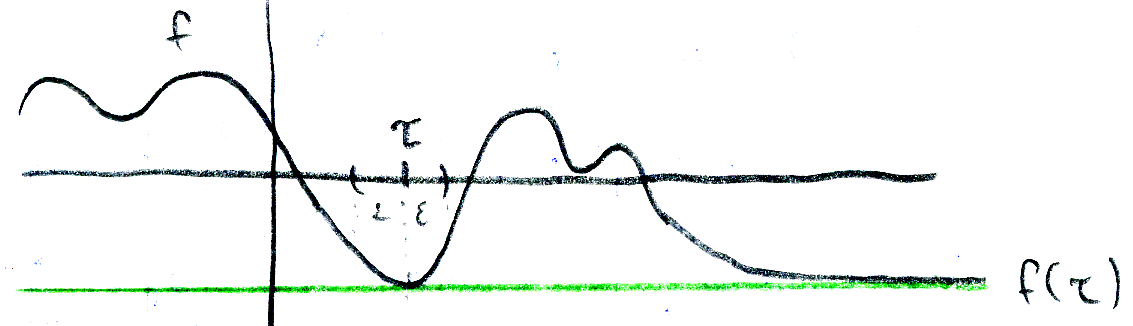
\includegraphics[width=1\textwidth]{./pics/MSTAT003.png}
			\caption{$\tau$ eindeutig, aber Infimum von $(\tau-\varepsilon,\tau+\varepsilon)$ ist auch $f(\tau)$!}
			\label{AbbMinimalstelleEindeutigNichtWohlsepariert}
		\end{center}
	\end{figure}
\end{beisp}

\begin{satz}\label{satz8.3}
	Seien $f,f_n,n\in\N$ aus $C(\R)$, $\tau_n\in A(f_n)\neq\emptyset~\forall n\geq N_0\in\N$ 
	(also $\tau_n$ ist eine Minimalstelle, ab einem gewissen Zeitpunkt $N_0$.)
	und $\tau\in A(f)$ sei wohl-separiert.
	Falls
	\begin{align}\label{eqSatz8.3_1}\tag{1}
		\big\Vert f_n-f\big\Vert\overset{\text{Def}}{=}\sup\limits_{t\in\R}\big|f_n(t)-f(t)\big|\overset{n\to\infty}{\longrightarrow}0
	\end{align}
	so folgt
	\begin{align*}
		\tau_n\overset{n\to\infty}{\longrightarrow}\tau
	\end{align*}
\end{satz}

\begin{proof}
	Sei $0<\varepsilon\overset{\text{oBdA}}{\in}\Q$. Es folgt:
	\begin{align*}
		s(\varepsilon)&:=\inf\limits\big\lbrace f(t):|t-\tau|\geq\varepsilon\big\rbrace
		\overset{\text{Def wohl-sep}}{>}
		f(\tau)\\
		\implies
		\delta&:=\delta(\varepsilon):=\frac{1}{3}\cdot\big(s(\varepsilon)-f(\tau)\big)>0\\
		\overset{\eqref{eqSatz8.3_1}}{\implies}
		\exists n_0&=n_0(\delta)\in\N:\forall n\geq n_0:
		\Vert f_n-f\Vert\leq\delta
	\end{align*}
	Für alle $n\geq\max\limits(N_0,n_0)$ gilt:\\
	Falls $t\in\R$ mit $|t-\tau|\geq\varepsilon$, so folgt:
	\begin{align*}
		f_n(t)-f_n(\tau)
		&=\underbrace{f_n(t)-f(t)}_{\geq\underbrace{-\underbrace{\Vert f_n-f\Vert}_{\leq\delta}}_{\geq-\delta}}+\underbrace{\underbrace{f(t)}_{\geq s(\varepsilon)}-f(\tau)}_{\geq s(\varepsilon)-f(\tau)=3\delta}+\underbrace{f(\tau)-f_n(\tau)}_{\geq-\delta}\\
		&\geq-\delta+3\cdot\delta-\delta\\
		&=\delta>0
	\end{align*}
	Es folgt
	\begin{align}\label{eqProofSatz8.3Stern}\tag{$\ast$}
		f_n(t)>f_n(\tau)\qquad\forall t\in\R\mit|t-\tau|\geq\varepsilon
	\end{align}
	Folglich gilt $|\tau_n-\tau|<\varepsilon$, denn sonst folgte aus \eqref{eqProofSatz8.3Stern}, dass
	$f_n(\tau_n)>f_n(\tau)$ im Widerspruch zu $\tau_n$ ist Minimalstelle von $f_n$.\\
	Somit gezeigt:
	\begin{align*}
		\forall\varepsilon\in\Q\cap(0,\infty):\exists m_0=m_0(\varepsilon):=\max\limits(N_0,n_0):\forall n\geq m_0:|t_n-\tau|<\varepsilon
	\end{align*}
\end{proof}

Satz \ref{satz8.3} lässt sich problemlos von $\R$ auf offene Intervalle $I=(a,b)$ übertragen.\nl
Für kompakte Intervalle $I=[a,b]$, $a<b\in\R$ muss $\tau$ nur eindeutig sein.
Es gilt:

\begin{satz}\label{satz8.4}
	Sei also $I=[a,b]$ kompaktes Intervall und seien $f,f_n,n\in\N$ aus $C(I)$. 
	Dann gilt:
	\begin{enumerate}[label=(\arabic*)]
		\item $\begin{aligned}
			A(f_n)\neq\emptyset\qquad\forall n\in\N
		\end{aligned}$
		\item Falls $\tau$ \underline{eindeutige} Minimalstelle von $f$ ist und falls
		\begin{align*}
			\Vert f_n-f\Vert_I:=\sup\limits_{t\in I}\big|f_n(t)-f(t)\big|\overset{n\to\infty}{\longrightarrow}0
		\end{align*}
		so gilt für \underline{jede} Auswahl $\tau_n\in A(f)$:
		$\tau_n\overset{n\to\infty}{\longrightarrow}\tau$
	\end{enumerate}
\end{satz}

%Ferger: "In irgendeinem der Seminarräumen ist mal eine Tafel von der Wand gefallen. Und ich möchte jetzt nicht unter so einer Tafel begraben liegen.
% Vielleicht ist das für einen Professor ein schöner Tod. Aber bitte jetzt noch nicht."
% "Ich bin ja von Natur aus etwas ängstlich. Es gab da mal so ein lustiges Lied und da singt der Sänger: "Leute seid nicht feige, lasst mich ...""

\begin{proof}
	\underline{Zeige (1):}\\
	Folgt, da jede stetige Funktion auf einem Kompaktum das Infimum annimmt.\nl
	\underline{Zeige (2):}\\
	$\tau$ ist wohl-separiert auf $I$, denn: 
	Angenommen, es wäre nicht so, also angenommen
	\begin{align*}
		\exists0<\varepsilon\in\Q:\inf\limits\big\lbrace f(t):t\in I:|t-\tau|\geq\varepsilon\big\rbrace=f(\tau)
	\end{align*}
	Die Menge $K_\varepsilon:=\lbrace t\in I:|t-\tau|\geq\varepsilon\rbrace$ ist kompakt.  
	Weil $f$ stetig ist, nimmt $f$ auf $K_\varepsilon$ ihr Infimum an, d.h.
	\begin{align*}
		\exists\sigma\in I:|\sigma-\tau|\geq\varepsilon\mit f(\sigma)=\inf\limits
		\big\lbrace f(t):t\in I:|t-\tau|\geq\varepsilon\big\rbrace
		=f(\tau)
	\end{align*}
	Also ist $\sigma$ eine \underline{weitere} Minimalstelle von $f$ (denn $\sigma$ und $\tau$ haben positiven Abstand zueinander) im Widerspruch zur Eindeutigkeit von $\tau$.\\
	Jetzt weiter wie im Beweis von Satz \ref{satz8.3}.
\end{proof}

Es ergeben sich nun mühelos Argmin-Theoreme für fast sichere Konvergenz:

\begin{satz}\label{satz8.5}
	Seien $M,M_n,n\in\N$ stochastische Prozesse über $(\Omega,\A,\P)$ mit Pfaden in $C(\R)$.
	Es gelte:
	\begin{enumerate}[label=(\arabic*)]
		\item $\begin{aligned}
			\tau\in A(M)
		\end{aligned}$ f.s. für eine Zufallsvariable $\tau$
		\item $\begin{aligned}
			\inf\limits\big\lbrace M(t):|t-\tau|\geq\varepsilon\big\rbrace>M(\tau)\text{ f.s.}\qquad\forall 0<\varepsilon\in\Q
		\end{aligned}$
		\item $\begin{aligned}
			\big\Vert M_n-M\big\Vert\overset{n\to\infty}{\longrightarrow}0\text{ f.s.}
		\end{aligned}$
	\end{enumerate}
	Dann gilt für jede Folge $(\tau_n)_{n\in\N}$ von Zufallsvariablen mit $\tau_n\in A(M_n)$ f.s.:
	$\tau_n\overset{n\to\infty}{\longrightarrow}\tau$ f.s.
\end{satz}

\begin{proof}
	Setze
	\begin{align*}
		\Omega_0:=\underbrace{\Big\lbrace\omega\in\Omega:\tau(\omega)\in A\big(M(\cdot,\omega)\big)\Big\rbrace}_{=:\big\lbrace\tau\in A(M)\big\rbrace\text{ Einsmenge wg (1)}}
		&\cap\bigcap\limits_{0<\varepsilon\in\Q}
		\underbrace{\Big\lbrace\inf\limits\big\lbrace M(t):|t-\tau|\geq\varepsilon\big\rbrace>M(\tau)\Big\rbrace}_{\text{Einsmenge wg. (2)}}\\
		&\cap\underbrace{\Big\lbrace\Vert M_n-M\Vert\overset{n\to\infty}{\longrightarrow}0\Big\rbrace}_{\text{Einsmenge wg (3)}}
		\cap\bigcap\limits_{n\geq1}\underbrace{\Big\lbrace\tau_n\in A(M_n)\Big\rbrace}_{\text{Einsmenge nach Vor.}}
	\end{align*}
	Erinnerung: Abzählbare Schnitte von Einsmengen sind Einsmengen.\\
	Dann gilt $\P(\Omega_0)=1$. 
	Da $\Omega_0\overset{\ref{satz8.3}}{\subseteq}\big\lbrace\tau_n\overset{n\to\infty}{\longrightarrow}\tau\big\rbrace$, folgt die Behauptung.
\end{proof}

Analog erhält man mit Satz \ref{satz8.4}:

\begin{satz}\label{satz8.6}
	Seien $M,M_n,n\in\N$ stochastische Prozesse über $(\Omega,\A,\P)$ mit Pfaden in $C(I)$,
	wobei $I$ kompaktes Intervall ist.
	Es gelte:
	\begin{enumerate}[label=(\arabic*)]
		\item Es gibt eine Zufallsvariable $\tau$, die f.s. eindeutige Minimalstelle von $M$ ist.
		\item $\begin{aligned}
			\Vert M_n-M\Vert_I\overset{n\to\infty}{\longrightarrow}0
		\end{aligned}$ f.s.
	\end{enumerate}
	Dann gilt für jede Folge $(\tau_n)_{n\in\N}$ von Zufallsvariablen mit $\tau_n\in A(M_n)$ f.s.:
	$\tau_n\overset{n\to\infty}{\longrightarrow}\tau$ f.s.
\end{satz}

\begin{proof}
	Setze
	\begin{align*}
		 \Omega_0&:=\lbrace\tau\text{ ist eindeutige Minimalst. v. }M\rbrace
		 \cap\Big\lbrace\Vert M_n-M\Vert_I\overset{n\to\infty}{\longrightarrow}0\Big\rbrace
		 \cap\bigcap\limits_{n\geq1}\Big\lbrace\tau_n\in A(M_n)\Big\rbrace\\
		 &\implies\P(\Omega_0)=1
	\end{align*}		
	Da $\Omega_0\overset{\ref{satz8.4}}{\subseteq}\Big\lbrace\tau_n\overset{n\to\infty}{\longrightarrow}\tau\Big\rbrace$, folgt die Behauptung.
\end{proof}

\subsection{Anwendung in der Statistik} %nonumber
Maximum-Likelihood-Schätzung in 1-parametrigen Exponentialfamilien
Seien $(X_n)_{n\geq1}$ i.i.d. Kopien von Zufallsvariablen $X$, (d.h. $X_i\sim X$ bzw. $X_i\overset{\L}{=}X$)
mit Werten im Messraum $(\X,\F)$ und mit $\mu$-Dichte 
\begin{align*}
	f_\theta(x)&=c(\theta)\cdot h(x)\cdot\exp\big(q(\theta)\cdot T(\theta)\big)
	\qquad\forall x\in\X,\theta\in\Theta\subseteq\R
\end{align*}

% Ferger:
% In der Statistik werden Beobachtungen als Realisierungen von Zufallsvariablen aufgefasst, also X(\omega)=Beobachtung für ein \omega\in\Omega
% X_i kann das Befragungsergebnis des $i$-ten Probanden sein
% Kann man die $X_i$ in der Theorie als Unabhhängigkeit annehmen? -> siehe Zeitreihenanalyse
% Natürlich ist es nicht immer gegeben, unabhängige Daten zu betrachten. Mann muss sich in jeder Situation fragen, ob diese Modellierung sinnvoll ist.

% Ferger zu mir: "Schreiben Sie auch meine Späße mit?"
% Ich: "Ja, natürlich!"
% Ferger: "Das ist bedenklich..."

Erinnere an Maximum-Likelihood-Schätzer (MLS /MLE):
\begin{align*}
	\ul{X}_n:=\big(X_1,\ldots,X_n\big)
\end{align*}
hat \textbf{Likelihood-Funktion}
\begin{align*}
	L_n(\theta,\ul{X}_n)&:=\prod\limits_{i=1}^n L\big(\theta,X_i\big)
	\qquad\mit\qquad
	L(\theta,x):=f_\theta(x)
\end{align*}
Zugehörige \textbf{$\log$-Likelihood-Funktion} ist
\begin{align*}
	l_n\big(\theta,\ul{X}_n\big)&:=\log\Big(L_n\big(\theta,\ul{X}_n\big)\Big)
	=\sum\limits_{i=1}^n\log\big(\theta,X_i\big)
	=\sum\limits_{i=1}^n l\big(\theta,X_i\big)\qquad\mit
\\
l(\theta,x)&:=\log\big(L(\theta,x)\big)=\log\big(f_\theta(x)\big)
\end{align*}
Der MLS für $\theta$ ist definiert durch
\begin{align*}
	\hat{\theta}_n
	:=\argmax\limits_{\theta\in\Theta}L_n\big(\theta,\ul{X}_n\big)
	%\overset{x\mapsto\log(x)\text{ streng monoton wachsend}}{=}
	\overset{(\ast)}{=}
	\argmax\limits_{\theta\in\Theta} l_n\big(\theta,\ul{X}_n\big)
	=\argmin\limits_{\theta\in\Theta}\underbrace{-\frac{1}{n}\cdot  l_n\big(\theta,\ul{X}_n\big)}_{=:S_n(\theta)}
\end{align*}
Die $(\ast)$-Gleichheit gilt, weil $x\mapsto\log(x)$ streng monoton wachsend und stetig ist.
\begin{align*}
	l(\theta,x)&=\log\big(c(\theta)\big)+\log\big(h(x)\big)+q(\theta)\cdot T(x)\\
	\implies S_n(\theta)&=-\log\big(c(\theta)\big)\underbrace{-\frac{1}{n}\cdot\sum\limits_{i=1}^n\log\big(h(X_i)\big)}_{\text{hängt \ul{nicht} von $\theta$ ab}}-q(\theta)\cdot\underbrace{\frac{1}{n}\cdot\sum\limits_{i=1}^n T(X_i)}_{=:\overline{T}_n}\\
	&=\underbrace{-\Big(\log\big(c(\theta)\big)+q(\theta)\cdot\overline{T}_n\Big)}_{=:M_n(\theta)}-\frac{1}{n}\cdot\sum\limits_{i=1}^n\log\big(h(X_i)\big)\\
	\implies\hat{\theta}_n
	&=\argmin\limits_{\theta\in\Theta} M_n(\theta)
\end{align*}

% Ferger zu den Schülern von Uni-Live: "Ich mach' auch sonst keine Späße. Und die Studenten sind auch immer leise."
%Ferger: "Ich komme aus einem 400-Einwohner Dorf."

\textbf{Annahme:}
\begin{enumerate}[label=(\arabic*)]
	\item $\Theta\subseteq\R$ ist kompaktes Intervall
	\item $q$ ist stetig auf $\Theta$ ($\implies c$ stetig, $c>0$).
	\item Sei $\theta_0$ der \textbf{wahre} Parameter, d.h. $X_i\sim f_{\theta_0}$
\end{enumerate}

Ziel: Zeige
\begin{align*}
	\hat{\theta}_n\overset{n\to\infty}{\longrightarrow}\theta_0
	\quad\P\text{-fast sicher}
	\qquad\forall \theta_0\in\Theta
\end{align*}
Das ist die sogenannte \textbf{starke Konsistenz} der Schätzerfolge $(\hat{\theta}_n)_{n\in\N}$.

% Ferger zu den Schülern: "Liebe Kinder, bitte nicht rauchen! Rauchen ist ungesund."
%Ferger: "Ich rauche in meinem Zimmer. Das ist verboten. Da ist ziviler ungehorsam. Ich warte immer noch, dass jemand zu mir kommt und sagt, dass das verboten. Und jetzt? Werfen Sie mich jetzt raus?
% Ich habe auch einen Hund in meinem Zimmer. Ist auch verboten."

Gemäß SGGZ gilt:
\begin{align}\label{eqUnderStarkeKonsistenz}
	\overline{T}_n\overset{n\to\infty}{\longrightarrow}&\E_{\theta_0}\big[T(X)\big]\quad\P\text{-fast sicher}\\
	\E_{\theta_0}\big[T(X)\big]
	&=\int\limits_\Omega T(X)\d\P_{\theta_0}
	\overset{\eqref{eqTrafo}}{=}
	\int\limits_{\X}T(x)\underbrace{\P_{\theta0}\circ X^{-1}}_{\text{hat $\mu$-Dichte}}(\d x)	
	\int\limits_{\X}T(x)\cdot f_{\theta_0}(x)~\mu(\d x)\nonumber
\end{align}

Erinnerung: 
\begin{align*}
	X_i:\big(\Omega,\A,\P_\theta)\to\big(\X,\F)
	\qquad
	X_i(\omega)\in\X\overset{\text{z.B.}}{=}\R
	\qquad
	\underline{X}_n:=\big(X_1,\ldots,X_n\big):\Omega\to\X^n
\end{align*}

Aus \eqref{eqUnderStarkeKonsistenz} folgt:
\begin{align*}
	M_n(\theta)\overset{n\to\infty}&{\longrightarrow}
	\underbrace{-\Big(\log\big(c(\theta)\big)+q(\theta)\cdot\E_{\theta_0}\big[T(X)\big]\Big)}_{=:M(\theta)=:M_{\theta_0}(\theta)}
	\quad\P\text{-f.s.}
	\qquad\forall\theta_0\in\Theta\\
	\Big|M_n(\theta)-M_{\theta_0}(\theta)\Big|
	&=\bigg|q(\theta)\cdot\Big(\overline{T}_n-\E_{\theta_0}\big[T(X)\big]\Big)\bigg|\\
	\implies
	\sup\limits_{\theta\in\Theta}\Big|M_n(\theta)-M_{\theta_0}(\theta)\Big|
	&=\underbrace{\left(\sup\limits_{\theta\in\Theta}\big|q(\theta)\big|\right)}_{=:c<\infty}
	\cdot\underbrace{\bigg|\Big(\overline{T}_n-\E_{\theta_0}\big[T(X)\big]\Big)\bigg|}_{\overset{n\to\infty}{\longrightarrow}0\text{ f.s.}}
\end{align*}
Die Bedingung (2) in Satz \ref{satz8.6} ist also erfüllt.

% Ferger hat am 18.01. Geburtstag

Falls $\theta_0$ eindeutige Minimalstelle von $M_{\theta_0}$ ist, so liefert Satz \ref{satz8.6} die starke Konsistenz von $(\hat{\theta}_n)_{n\in\N}$.
Zusammenfassung in:

\begin{satz}\label{satz8.7}
	 Im Modell (Exponential-Familie) sei $\Theta\subseteq\R$ kompaktes Intervall,
	 $q$ sei stetig und der wahre Parameter $\theta_0$ sei eindeutige Minimalstelle der Funktion
	 \begin{align*}
	 	M_{\theta_0}(\theta)
	 	&=-\log\big(c(\theta)\big)-q(\theta)\cdot c(\theta)\cdot\int\limits T(x)\cdot h(x)\cdot\exp\big(q(\theta_0)\cdot T(x)\big)~\mu(\d x)
	 	\qquad\forall\theta\in\Theta
	 \end{align*}
	 (Das ist eine implizite Forderung an die Verteilungsannahmen (VA).)
	 Und sei 
	 \begin{align*}
	 	\hat{\theta}_n=\argmin\limits_{\theta\in\Theta} M_n(\theta)
	 	\qquad\mit\qquad
	 	M_n(\theta)=-\log\big(c(\theta)\big)-q(\theta)\cdot\frac{1}{n}\cdot\sum\limits_{i=1}^n T(X_i)
	 \end{align*}
	 Dann gilt:
	 \begin{align*}
	 	\hat{\theta}_n\overset{n\to\infty}{\longrightarrow}
	 	\theta_0\quad\P\text{-f.s.}\qquad\forall\theta_0\in\Theta
	 \end{align*}
\end{satz}

\begin{proof}
	Folgt aus Satz \ref{satz8.6}.
\end{proof}

%Ferger: "Stellen wir uns mal konkret einen Hilbertraum vor."

Vom theoretischen Standpunkt aus ist die Kompaktheitsannahme an $\Theta$ sehr stark.
Allerdings ist dies für den Anwender keine signifikante Einschränkung.
Dafür aber neben der Stetigkeit von $q$ \underline{keine} weitere "Glattheitsannahmen".
Sind solche Glattheitsannahmen aber gegeben, so lässt sich zeigen, dass $\theta_0$ tatsächlich eindeutiger (und im Fall $\Theta=\R$ wohl-separierte) Minimalstelle von $M_{\theta_0}$ ist. 

\subsection{Anwendung in der Change-Point-Analyse} %8.2
Betrachten des Change-Point-Modell aus Kapitel 7.1:
$X_{1,n},\ldots,X_{n,n},n\in\N$ seien unabhängige reelle Zufallsvariablen mit 
\begin{align*}
	\left\lbrace\begin{array}{ll}
		X_{i,n}\text{ i.i.d }\sim(\mu,\sigma^2), &\falls 1\leq i\leq\tau_n\\
		X_{i,n}\text{ i.i.d }\sim(\nu,\tau^2), &\falls \tau_n< i\leq\tau_n\\
	\end{array}\right.,\qquad\mu\neq\nu
\end{align*}
Mit $\tau_n\in\big\lbrace1,\ldots,n-1\big\rbrace$ unbekannter \textbf{Wechselzeitpunkt}.
\begin{align*}
	\underbrace{X_1,\ldots,X_{\tau_n}}_{\text{pre-change variables}},\underbrace{X_{\tau_n+1},\ldots,X_n}_{\text{post-change variables}}
\end{align*}

\underline{Ziel:} Schätzung von $\tau$\\
Schreibe im Folgenden: $X_i\equiv X_{i,n}$
\begin{align*}
	S_k&:=\sum\limits_{i=1}^k\big(X_i-\overline{X}_n\big) &\forall& 0\leq k\leq n\\
	\overline{X}_n&:=\frac{1}{n}\cdot\sum\limits_{i=1}^n X_i &\forall& n\in\N\\
	\theta_n&:=\frac{\tau_n}{n} &\forall& n\in\N
\end{align*}

Eine elementare Rechnung zeigt (zur Übung):
\begin{align}\label{eqUnder8.2_1}\tag{1}
	\E[S_k]
	&=\left\lbrace\begin{array}{cll}
		k\cdot(1-\theta_n)\cdot(\mu-\nu), &\falls 0\leq k\leq\tau_n &\text{monoton wachsend}\\
		(n-k)\cdot\theta_n\cdot(\mu-\nu), &\falls\tau_n<k\leq n &\text{monoton fallend}
	\end{array}\right.\\\nonumber
	\big|\E[S_k]\big|
	&=\left\lbrace\begin{array}{cll}
		k\cdot(1-\theta_n)\cdot|\mu-\nu|, &\falls 0\leq k\leq\tau_n &\text{monoton wachsend}\\
		(n-k)\cdot\theta_n\cdot|\mu-\nu|, &\falls\tau_n<k\leq n &\text{monoton fallend}
	\end{array}\right.\\
	&\implies\tau_n=\argmax\limits_{0\leq k\leq n}\big|\E[S_k]\big|\nonumber
\end{align}

Daraus folgt, dass $\E[S_k]$ (in Abhängigkeit von $k$) erst monoton wachsend und ab $k=\tau_n$ monoton fallend ist.

\begin{figure}[H] % oder ht!
	\begin{center}
		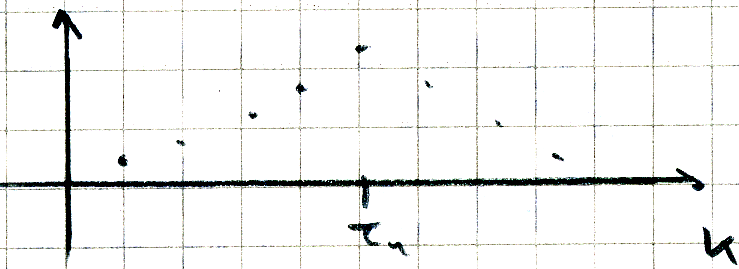
\includegraphics[width=1\textwidth]{./pics/MSTAT004.png}
		\caption{Plot von $\E[S_k]$}
		%\label{Abb}
	\end{center}
\end{figure}

Dies motiviert folgenden Schätzer (ersetze unbekannte $\big|\E[S_k)\big]$ durch bekannte $|S_k|$):
\begin{align*}
	\hat{\tau}_n:=\argmax\limits_{0\leq k\leq n}\big|S_k\big|
\end{align*}
Im Folgenden sei $\tau_n=\lfloor n\cdot\theta\rfloor,\theta\in(0,1)$.
Wir zeigen:
\begin{align*}
	\hat{\theta}_n:=\frac{\hat{\tau}_n}{n}\overset{n\to\infty}{\longrightarrow}\theta\qquad\P\text{-f.s.}
\end{align*}

\textbf{Annahme:} Wir nehmen die sogenannte \textbf{Momentenbedingung an}, d.h.
\begin{align*}
	\mu_p:=\E\Big[\big|X_{\tau_n}\big|^p\Big]<\infty,
	\qquad
	\nu_p:=\E\Big[\big|X_{\tau_n+1}\big|^p\Big]<\infty
\end{align*}

Sei $M_n:=$ Polygonzug durch $\left(\frac{k}{n},\frac{1}{n}\cdot S_k\right)$, $0\leq k\leq n$.
Dann folgt aus Lemma \ref{lemma7.17}:
\begin{align*}
	\hat{\theta}_n&:=\argmax\limits_{0\leq t\leq 1}\big|M_n(t)\big|\\
	M_n(t)&~=\frac{1}{n}\cdot S_{\lfloor n\cdot t\rfloor}+\big(n\cdot t-\lfloor w\cdot t\rfloor\big)\cdot\Big(S_{\lfloor n\cdot t\rfloor+1}-S_{\lfloor n\cdot t\rfloor+1}\Big) &\forall 0\leq t\leq 1\\
	\E\big[M_n(t)\big]&~=\frac{1}{n}\cdot\E\Big[ S_{\lfloor n\cdot t\rfloor}\Big]+\big(n\cdot t-\lfloor w\cdot t\rfloor\big)\cdot
	\Big(\E\Big[S_{\lfloor n\cdot t\rfloor+1}\Big]-\E\Big[S_{\lfloor n\cdot t\rfloor+1}\Big]\Big) &\forall 0\leq t\leq 1\\
\end{align*}

Sei $\overline{M}_n(t):=\E\big[M_n(t)\big),0\leq t\leq 1$. 
Dann ist $\overline{M}_n$ ein Polygonzug durch die Punkte $\left(\frac{k}{n},\frac{1}{n}\cdot\E[S_k]\right)$ $0\leq k\leq n$.
Da wegen \eqref{eqUnder8.2_1} 
\begin{align*}
	\overline{M}_n\left(\frac{k}{n}\right)
	&=\frac{1}{n}\cdot\E\big[S_k\big]
	\overset{\eqref{eqUnder8.2_1}}
	=
	\left\lbrace\begin{array}{cl}
		\frac{k}{n}\cdot(1-\theta_n)\cdot(\mu-\nu) &\falls \frac{k}{n}\leq\frac{\tau_n}{n}=\theta_n\\
		\left(1-\frac{k}{n}\right)\cdot\theta_n\cdot(\mu-\nu), & \falls \frac{k}{n}>\theta_n
	\end{array}\right.
\end{align*}
folgt
\begin{align*}
	\overline{M}_n\left(t\right)
	&=\left\lbrace\begin{array}{cl}
		t\cdot(1-\theta_n)\cdot(\mu-\nu) &\falls t\leq\theta_n\\
		\left(1-t\right)\cdot\theta_n\cdot(\mu-\nu), & \falls \frac{k}{n}>\theta_n
	\end{array}\right.
\end{align*}
Beachte $\theta-\frac{1}{n}<\theta_n=\frac{\lfloor n\cdot\theta\rfloor}{n}=\theta$.
Eine Fallunterscheidung ($t\leq\theta_n$; $\theta_n<t\leq\theta$; $t>\theta$) liefert
\begin{align}\label{eqUnder8.2_2}\tag{2}
	\big\Vert\overline{M}_n-M\big\Vert
	&=\sup\limits_{0\leq t\leq 1}\Big|\overline{M}_n(t)-M(t)\Big|
	\leq 2\cdot|\mu-\nu|\cdot n^{-1}\overset{n\to\infty}{\longrightarrow}0\text{ wobei}\\\nonumber
	M(t)&=\left\lbrace\begin{array}{cl}
		t\cdot(1-\theta)\cdot(\mu-\nu) ,&\falls 0\leq t\leq\theta\\
		(1-t)\cdot\theta\cdot(\mu-\nu), &\falls \theta<t\leq 1
	\end{array}\right.\\\nonumber
	|M(t)|&=\left\lbrace\begin{array}{cl}
		t\cdot(1-\theta)\cdot|\mu-\nu| ,&\falls 0\leq t\leq\theta\\
		(1-t)\cdot\theta\cdot|\mu-\nu|, &\falls \theta<t\leq 1
	\end{array}\right.
\end{align}

\begin{figure}[H]
	\begin{center}
		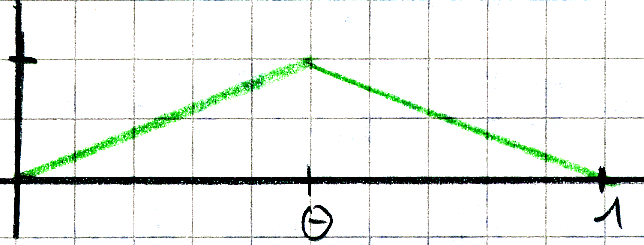
\includegraphics[width=1\textwidth]{./pics/MSTAT005.png}
		\caption{Plot von $M(t)$}
		%\label{AbbTitel}
	\end{center}
\end{figure}

Somit ist dieses $\theta$ charakterisierbar als Maximalstelle:
\begin{align*}
	\theta=\argmax\limits_{0\leq t\leq 1}\big|M(t)\big|
\end{align*}

Zeige:
\begin{align*}
	\big\Vert M_n-M\big\Vert
	&=\sup\limits_{0\leq t\leq 1}\big|M_n(t)-M(t)\big|\overset{n\to\infty}{\longrightarrow}0\quad\P\text{-f.s.}
\end{align*}
Da
\begin{align}\label{eqUnder8.2_3}\tag{3}
	0\leq\big\Vert M_n-M\big\Vert\leq\big\Vert M_n-\overline{M}_n\big\Vert+\underbrace{\big\Vert\overline{M}_n-M\big\Vert}_{
		\stackrelnew{\eqref{eqUnder8.2_2}}{n\to\infty}{\longrightarrow}0
	}
\end{align}

Betrachte den ersten Summanden
\begin{align}\label{eqUnder8.2_4}\tag{4}
	\big\Vert M_n-\overline{M}_n\big\Vert
	=\sup\limits_{0\leq t\leq 1}&\big|M_n(t)-\overline{M}_n(t)\big|
	\overset{\ref{lemma7.17}}{=}
	\max\limits_{0\leq k\leq n}\bigg|\underbrace{M_n\left(\frac{k}{n}\right)}_{=\frac{1}{n}\cdot S_k}-\underbrace{\overline{M}_n\left(\frac{k}{n}\right)}_{=\frac{1}{n}\cdot\E[S_k]}\bigg|\\\nonumber
	\frac{1}{n}\cdot S_k
	&=\frac{1}{n}\cdot\sum\limits_{i=1}^k\big(X_i-\overline{X}_n\big)
	=\frac{1}{n}\cdot\sum\limits_{i=1}^k X_i-\frac{k}{n^2}\cdot\sum\limits_{i=1}^n X_i\\\nonumber
	\implies
	M_n\left(\frac{k}{n}\right)-\overline{M}_n\left(\frac{k}{n}\right)
	\overset{\text{Lin}}&=
	\frac{1}{n}\cdot\sum\limits_{i=1}^n\underbrace{\Big(X_i-\E\big[X_i\big]\Big)}_{=:Z_i}-\frac{k}{n^2}\cdot\sum\limits_{i=1}^n\underbrace{\Big(X_i-\E\big[X_i\big]\Big)}_{=Z_i}\\\nonumber
	\implies
	\left|M_n\left(\frac{k}{n}\right)-\overline{M}_n\left(\frac{k}{n}\right)\right|
	\overset{\text{DU}}&\leq
	\frac{1}{n}\cdot\underbrace{\bigg|\sum\limits_{i=1}^n\underbrace{\Big(X_i-\E\big[X_i\big]\Big)}_{=:Z_i}\bigg|}_{
		\leq\max\limits_{0\leq k\leq n}\left|\sum\limits_{i=1}^k Z_i\right|
	}+\underbrace{\frac{k}{n^2}}_{\leq\frac{1}{n}}\underbrace{\cdot\bigg|\sum\limits_{i=1}^n\underbrace{\Big(X_i-\E\big[X_i\big]\Big)}_{=Z_i}\bigg|}_{
		\leq\max\limits_{0\leq k\leq n}\left|\sum\limits_{i=1}^k Z_i\right|
	}\\\nonumber
	&\leq2\cdot\frac{1}{n}\cdot\max\limits_{0\leq k\leq n}\left|\sum\limits_{i=1}^k Z_i\right|\\
	\implies\label{eqUnder8.2_5}\tag{5}
	&\max\limits_{0\leq k\leq n}\left|M_n\left(\frac{k}{n}\right)-\overline{M}_n\left(\frac{k}{n}\right)\right|
	\leq 2\cdot\frac{1}{n}\cdot\max\limits_{0\leq k\leq n}\left|\sum\limits_{i=1}^k Z_i\right|
\end{align}

Es ist
\begin{align*}
	T_k=\sum\limits_{i=1}^k Z_i\qquad 0\leq k\leq n
\end{align*}
ein Martingal bzgl. Filtration 
\begin{align*}
	\F_k:=\sigma\big(Z_1,\ldots,Z_k\big) &\qquad\forall 1\leq k\leq n,\qquad \F_0:=\lbrace\emptyset,\Omega\rbrace
\end{align*}
Ist Martingal, weil
\begin{align*}
	\E\Big[T_{k+1}~\Big|~\F_k\Big]
	&=\E\left.\left[\sum\limits_{i=1}^k Z_i+Z_{k+1}~\right|~\F_k\right]
	=\underbrace{\E\bigg[\overbrace{\sum\limits_{i=1}^k Z_i}^{\text{ist $\F_K$-messbar}}~\bigg|~\F_k\bigg]}_{=T_k}+\underbrace{\E\Big[ Z_{k+1}~\Big|~\F_k\Big]}_{=\E[Z_{k+1}]=0}
\end{align*}

Es folgt aus der bedingten Jensenungleichung, dass $\left(|T_k|^p,\F_k\right)_{0\leq k\leq n}$ ein nicht-negatives Submartingal ist.
\begin{align}\nonumber
	\P\Big(\big\Vert M_n-\overline{M}_n\big\Vert\geq\varepsilon\Big)
	\overset{\eqref{eqUnder8.2_4}+\eqref{eqUnder8.2_5}}&{\leq}
	2\cdot\frac{1}{n}\cdot\max\limits_{0\leq k\leq n}\big|T_k\big|\\\nonumber
	&\leq\P\left(\max\limits_{0\leq k\leq n}\big|T_k\big|\geq\frac{1}{2}\cdot n\cdot\varepsilon\right)\\\nonumber
	\overset{u\mapsto u^p\uparrow}&\leq
	\P\left(\left(\max\limits_{0\leq k\leq n}\big|T_k\big|\right)^p\geq\left(\frac{1}{2}\cdot n\cdot\varepsilon\right)^p\right)\\\nonumber
	&=\P\left(\max\limits_{0\leq k\leq n}\big|T_k\big|^p\geq\left(\frac{1}{2}\cdot n\cdot\varepsilon\right)^p\right)\\\nonumber
	\implies
	\P\Big(\big\Vert M_n-\overline{M}_n\big\Vert\geq\varepsilon\Big)
	&\leq\P\bigg(\max\limits_{0\leq k\leq n}\underbrace{\big|T_k\big|^p}_{\text{Submartingal}}\geq\underbrace{2^{-p}\cdot n^p\cdot\varepsilon^p}_{=:y>0}\bigg)\\\nonumber
	\overset{\text{Doob-Ungl}}&\leq
	y^{-1}\cdot\E\left[\big|T_n\big|^p\right]\\
	&=2^p\cdot n^{-p}\cdot\varepsilon^{-p}\cdot\E\left[\left|\sum\limits_{i=1}^n Z_i\right|^p\right]\label{eqUnder8.2_6}\tag{6}
\end{align}

Es gilt folgende \textbf{Momenten-Ungleichung} (vergleiche (1.6) in Ferger (2014), \textit{Optimal constants in the Marcinkiewicz-Zygmund-inequalities, statistics and propability letters} Ausgabe 84, Seiten 96 bis 101)

\begin{align*}
	\E\left[\left|\sum\limits_{i=1}^n Z_i\right|^p\right]
	\overset{(1.6)}{\leq}
	C_p\cdot n^{\frac{p}{2}}\cdot\sum\limits_{i=1}^n\E\Big[|Z_i|^p\Big]
\end{align*}

Erinnerung:
\begin{align*}
	Z_i&=X_i-\E[X_i]\\
	\implies
	|Z_i|^p&=\big|X_i-\E[X_i]\big|^p\\
	\implies
	\big|X_i-\E[X_i]\big|^p
	\overset{C_r\text{ Ungl}}&\leq
	c_p\cdot\Big(|X_i|^p+\underbrace{\big|\E[X_i]\big|^p}_{\overset{\text{Jensen}}{\leq}\E\big[|X_i|^p\big]}\Big)\\
	\implies
	\E\Big[|Z_i|^p\Big]
	&\leq c_p\cdot\left(\E\big[|X_i|^p\big]+\E\big[|X_i|^p\big]\right)\\
	&\leq 2\cdot c_p\cdot\underbrace{\E\Big[|X_i|^p\Big]}_{\leq\max\lbrace\mu_p,\nu_p\rbrace}
\end{align*}
Somit gibt es eine Konstante $D_p$ so, dass
\begin{align*}
	\E\left[\left|\sum\limits_{i=1}^n Z_i\right|^p\right]
	\overset{(1.6)}&{\leq}
	C_p\cdot n^{-\frac{p}{2}}\cdot\sum\limits_{i=1}^n\underbrace{\E\Big[|Z_i|^p\Big]}_{\leq D_p}\\
	\implies
	\E\left[\left|\sum\limits_{i=1}^n Z_i\right|\right]
	&\leq\tilde{c}_p\cdot n^{\frac{p}{2}}\\
	\overset{\eqref{eqUnder8.2_6}}{\implies}
	\P\Big(\big\Vert M_m-\overline{M}_n\big\Vert\geq\varepsilon\Big)
	&\leq\overline{c}_p\cdot\varepsilon^{-p}\qquad\forall\varepsilon>0
\end{align*}

Nun bilden wir die Reihe dieser Wahrscheinlichkeiten und erhalten Konvergenz für $p>2$:
\begin{align*}
	\overset{p>2}{\implies}
	\sum\limits_{n=1}^\infty\P\Big(\big\Vert M_m-\overline{M}_n\big\Vert\geq\varepsilon\Big)<\infty\qquad\forall\varepsilon>0
\end{align*}

Es gilt ganz allgemein für eine Folge $(\xi_n)_{n\in\N}$ von Zufallsvariablen (folgt aus dem Borel-Cantelli-Lemma):
\begin{align*}
	\left(\forall\varepsilon>0:\sum\limits_{n=1}^\infty\P\Big(|\xi_n|\geq\varepsilon\Big)<\infty\right)\implies\xi_n\overset{n\to\infty}{\longrightarrow}0\text{ f.s.}
\end{align*}

Also erhalten wir
\begin{align*}
	\big\Vert M_n-\overline{M}_n\big\Vert\overset{n\to\infty}{\longrightarrow}0\text{ f.s.}\\
	\overset{\eqref{eqUnder8.2_2}+\eqref{eqUnder8.2_3}}{\implies}
	\big\Vert M_n-M\big\Vert\overset{n\to\infty}{\longrightarrow}0\text{ f.s.}
\end{align*}

Da
\begin{align*}
	\Big\Vert\big|M_n\big|-\big|M\big|\Big\Vert\leq\big\Vert M_n-M\big\Vert
\end{align*}
folgt
\begin{align*}
	\Big\Vert\big|M_n\big|-\big|M\big|\Big\Vert\overset{n\to\infty}&{\longrightarrow}0\text{ f.s.}\\
	\implies	
	\Big\Vert-\big|M_n\big|-\big(-\big|M\big|)\Big\Vert\overset{n\to\infty}&{\longrightarrow}0\text{ f.s.}\\
	\implies
	\hat{\theta}_n
	&=\argmax\limits_{0\leq t\leq 1}\big|M_n(t)\big|
	=\argmin\limits_{0\leq t\leq 1}-\big|M_n(t)\big|
\end{align*}
Also hat $-|M|$ eindeutige Minimalstelle $\theta$.
Aus Satz \ref{satz8.6} folgt nun $\hat{\theta}\overset{n\to\infty}{\longrightarrow}\theta$ f.s.\\
(In Satz \ref{satz8.6} verwende: $M_n\hat{=}-|M_n|$, $M\hat{=}|M|$, $\tau\hat{=}\theta$)

\begin{bemerkung}
	Betrachte eine endliche Beobachtungsfolge:\\
	$X_1,X_2,\ldots,X_\tau,X_{\tau+1},X_{\tau+},\ldots,X_n\qquad n>\tau$\\
	Hier braucht man keinen doppelten Index.
	Vergrößert man aber nun $n$, dann geht der Anteil an der Gesamtstichprobe gegen 0, also $\frac{\tau}{n}\longrightarrow0$.
\end{bemerkung}

Zusammenfassung unserer Überlegungen in
\begin{satz}\label{satz8.8}
	Sei $\theta\in(0,1),\mu\neq\nu,\mu_p<\infty,\nu_p<\infty$ für ein $p>2$.
	Dann gilt:
	\begin{align*}
		\hat{\theta}_n
		&=\frac{1}{n}\cdot\underbrace{\argmax\limits_{0\leq k\leq n}\left|\sum\limits_{i=1}^k\big(X_i-\overline{X}_n\big)\right|}_{=\hat{\tau}_n}\overset{n\to\infty}{\longrightarrow}0\text{ f.s.}
	\end{align*}
\end{satz}

\begin{bemerkung}
	 Es gilt \underline{nicht}, dass $\hat{\tau}_n-\tau_n\overset{n\to\infty}{\longrightarrow}0$ f.s.
	 Tatsächlich gilt:
	 \begin{align*}
	 	\hat{\tau}_n-\tau_n\overset{\L}{\longrightarrow} T
	 \end{align*}
	 wobei $T$ die f.s. eindeutige Maximalstelle einer \textit{2-seitigen Irrfahrt / Random Walk} auf $\Z$ ist
	 (vergleiche D.F. (1994) \textit{Asymptotic distribution theory of change-point estimators} veröffentlicht in \textit{Mathematical methods in statics 3}, Seiten 362 bis 378).
\end{bemerkung}

Nächstes Ziel: Unter welchen Bedingungen gilt
\begin{align*}
	Z_n\overset{L}{\longrightarrow}Z\text{ in }\big(C(\R),d\big)
	\implies\argmin\limits_{t\in\R}Z_n(t)\overset{\L}{\longrightarrow}\argmin\limits_{t\in\R}Z(t)
\end{align*}

Folgender Satz gibt Antwort.

\begin{satz}\label{satz8.9}
	Seien $Z,Z_n,n\in\N$ stochastische Prozesse mit Pfaden in $C(\R)$ über $(\Omega,\A,P)$,
	wobei $A(Z)$ 
	\footnote{$A(Z)$ ist eine \textit{random closed set (RCS)}} 
	und $A(Z_n)$ für alle $n\in\N$ nichtleer sind.
	Ferner sei $\sigma_n$ eine Zufallsvariable mit $\sigma_n\in A(Z_n)$.
	Dann gilt: Falls
	\begin{align}\label{eqSatz8.9_1}\tag{1}
		Z_n\overset{L}{\longrightarrow} Z\text{ in }\big(C(\R),d\big)
	\end{align}
	so folgt
	\begin{align}\label{eqSatz8.9_a}\tag{a}
		\limsup\limits_{n\to\infty}\P\big(\sigma_n\in K\big)\leq\mu^\ast(K)\qquad\forall K\in\mathcal{K}:=\big\lbrace K\subseteq\R:K\text{ kompakt}\big\rbrace
	\end{align}
	wobei $\mu^\ast$
	\footnote{$\mu^\ast$ ist die \textit{Kapazitätsfunktion von $A(Z)$} und damit insbesondere eine \textit{Choquet-Kapazität}.
	Beachte, dass $\mu^\ast$ i.d.R. \underline{kein} W-Maß.}	
	die sogenannte \textbf{hitting-probability} ist:
	\begin{align*}
		\mu^\ast:\mathcal{K}\to[0,1],\qquad
		\mu^\ast(K)=\P\big(A(Z)\cap K\neq\emptyset\big)
	\end{align*}
	Gilt zusätzlich, dass $(\sigma_n)_{n\in\N}$ \textbf{stochastisch beschränkt} ist, d.h. 
	\begin{align}\label{eqSatz8.9_2}\tag{2}
		\lim\limits_{j\to\infty}\limsup\limits_{n\to\infty}\P\Big(\big|\sigma_n\big|>j\Big)=0
	\end{align}
	so folgt
	\begin{align}\label{eqSatz8.9_b}\tag{b}
		\limsup\limits_{n\to\infty}\P\big(\sigma_n\in F\big)\leq\mu^\ast(F)\qquad\forall F\in\F(\R):=\big\lbrace F\subseteq\R:F\text{ abgeschlossen}\big\rbrace
	\end{align}
	Falls zusätzlich $A(Z)=\lbrace\sigma\rbrace$ für eine Zufallsvariable $\sigma$
	(d.h. $Z$ hat f.s. eine eindeutige Minimalstelle, nämlich $\sigma$), dann gilt
	\begin{align}\label{eqSatz8.9_c}\tag{c}
		\sigma_n\overset{L}{\longrightarrow}\sigma\text{ in }\R.
	\end{align}
\end{satz}

%Ferger: "Ich weiß nicht mehr wie ich drauf gekommen bin. Aber ich bin darauf gekommen. Da habe ich mich gefreut wie so ein Brötchen."
%Ferger: "Müssen Sie nicht mitschreiben, ich will jetzt hier nur zu einer didaktischen Meisterleistung auflaufen."

\begin{proof}
	\underline{Zeige \eqref{eqSatz8.9_a}:}\\
	Sei $K$ kompakt. Dann gilt:
	\begin{align}\label{eqProofSatz8.9_i}\tag{i}
		\big\lbrace\sigma_n\in K\big\rbrace
		&\subseteq\left\lbrace\inf\limits{t\in K} Z_n(t)\leq\inf\limits_{t\not\in K} Z_n(t)\right\rbrace\\
		&\subseteq\left\lbrace\inf\limits_{t\in K} Z_n(t)\leq\inf\limits_{t\in K^C\cap I_j}Z_n(t)\right\rbrace\label{eqProofSatz8.9_ii}\tag{ii}
	\end{align}
	wobei $I_j:=[-j,j],j\in\N$.\nl
	\underline{Zeige \eqref{eqProofSatz8.9_i}:}\\
	Sei $\sigma_n\in K$ und angenommen
	\begin{align}\label{eqProofSatz8.9Stern}\tag{$\ast$}
		\inf\limits_{t\in K} Z_n(t)>\inf\limits_{t\in K^C} Z_n(t)
	\end{align}
	Dann gilt:
	\begin{align*}
		Z_n(\sigma_n)
		\overset{\sigma_n\in K}&\geq
		\inf\limits_{t\in K} Z_n(t)
		\overset{\eqref{eqProofSatz8.9Stern}}>
		\inf\limits_{t\in K^C} Z_n(t)
		\overset{K^C\subseteq\R}\geq
		\inf\limits_{t\in\R} Z_n(t)
		\overset{\sigma_n\in A(Z_n)}=
		Z(\sigma_n)
	\end{align*}
	Das ist ein Widerspruch, weshalb \eqref{eqProofSatz8.9_i} folgt.\nl
	Gleichung \eqref{eqProofSatz8.9_ii} folgt aus 
	\begin{align*}
		\inf\limits_{t\in K^C} Z_n(t)\leq\inf\limits_{t\in K^C\cap I_j}Z_n(t).
	\end{align*}
	Sei $K_j:=[-k_j,k_j]$ mit $k_j\in\N$ so, dass $K_j\supseteq K\cup I_j$.
	Für jedes $M\subseteq K_j$ gilt:
	Die Abbildung $f\mapsto\inf\limits_{t\in M} f(t)$ ist stetig auf $\big(C(K_j),\Vert\cdot\Vert_{K_j}\big)$,
	denn:
	\begin{align*}
		\left|\inf\limits_{t\in M} f(t)-\inf\limits_{t\in M}g(t)\right|
		&\leq \Vert f-g\Vert_M
		\leq\Vert f-g\Vert_{K_j}
	\end{align*}
	Daraus folgt, dass die Abbildung
	\begin{align*}
		H_j:\left(C\big(K_j\big),\Vert\cdot\Vert_{K_j}\right)\to\R,\qquad
		f\mapsto\inf\limits_{t\in K} f(t)-\inf\limits_{t\in K^C\cap I_j} f(t)
	\end{align*}
	stetig ist, denn $K^C\cap I_j\subseteq I_j\subseteq K\cup I_j\subseteq K_j$.
	Somit folgt aus Satz \ref{satz7.23} und aus dem CMT \ref{satz4.10ContinuousMappingTheorem}:
	\begin{align}\label{eqProofSatz8.9_iii}\tag{iii}
		H_j(Z_n)\overset{\L}{\longrightarrow} H_j(Z)\qquad\forall j\in\N
	\end{align}
	Aus \eqref{eqProofSatz8.9_i} und \eqref{eqProofSatz8.9_ii} folgt:
	\begin{align}\nonumber
		\P\Big(\big\lbrace\sigma_n\in K\big\rbrace\Big)
			&\leq\P\Bigg(\Bigg\lbrace\underbrace{\inf\limits_{t\in K} Z_n(t)-\inf\limits_{t\in K^C\cap I_j}Z_n(t)}_{=H_j(Z_n)}\leq0\Bigg\rbrace\Bigg)\\\nonumber
		\implies		
		\limsup\limits_{n\to\infty}\P\big(\sigma_n\in K\big)
		\overset{\eqref{eqProofSatz8.9_i}+\eqref{eqProofSatz8.9_ii}}&\leq
		\limsup\limits_{n\to\infty}\P\Big(H_j(Z_n)\in\underbrace{(-\infty,0]}_{\in\F(\R)}\Big)\\\nonumber
		\overset{\eqref{eqProofSatz8.9_iii}+\text{Portmannteau}}&\leq
		\P\Big(H_j(Z)\in(-\infty,0]\Big)\\
		\overset{\text{Def }H_j}&=
		\P\bigg(\underbrace{\bigg\lbrace\inf\limits_{t\in K}Z(t)\leq\inf\limits_{t\in K^C\cap I_j}Z(t)\bigg\rbrace}_{=:E_j}\qquad\forall j\in\N\label{eqProofSatz8.9_iv}\tag{iv}
	\end{align}
	Da $E_j$ monoton fallend ist, folgt (mit $\sigma$-Stetigkeit von oben):
	\begin{align*}
		\lim\limits_{j\to\infty}\P(E_j)
		&=\P\left(\bigcap\limits_{j\in\N}E_j\right)\\
		&=\P\left(\inf\limits_{t\in K}Z(t)\leq\inf\limits_{t\in K^C\cap I_j}Z(t)~\forall j\in\N\right)\\
		&\leq \P\bigg(\inf\limits_{t\in K}Z(t)\leq\underbrace{\inf\limits_{j\in\N}\inf\limits_{t\in K^C\cap I_j}Z(t)}_{=\inf\limits_{\bigcup\limits_{j\in\N}\big(K^C\cap I_j\big)}Z(t)}\bigg)\\
		\overset{\bigcup\limits_j(K^C\cap I_j)=K^C\cap\bigcap\limits_j I_j=K^C\cap\R}&=
		\P\bigg(\underbrace{\bigg\lbrace\inf\limits_{t\in K} Z(t)\leq\inf\limits_{t\in K^C} Z(t)\bigg\rbrace}_{=:E}\bigg)
	\end{align*}
	Dahinter steckt die allgemeine Rechenregel
	\begin{align*}
		\inf\limits_{t\in A\cup B}f(t)=\inf\limits\left\lbrace\inf\limits_A f,\inf\limits_B f\right\rbrace.
	\end{align*}
	Grenzübergang $j\to\infty$ in \eqref{eqProofSatz8.9_iv} liefert:
	\begin{align}\label{eqProofSatz8.9Plus}\tag{+}
		\limsup\limits_{n\to\infty}\P\big(\sigma_n\in K\big)
		\leq\lim\limits_{j\to\infty}\P(E_j)\leq\P(E)
	\end{align}
	Schließlich gilt
	\begin{align}\label{eqProofSatz8.9_v}\tag{v}
		E\subseteq\big\lbrace A(Z)\cap K\neq\emptyset\big\rbrace
	\end{align}
	denn:
	\begin{align*}
		&\inf\limits_{t\in K}Z(t)
		\leq\inf\limits_{t\in K^C} Z(t)\\
		&\implies
		\inf\limits_\R Z(t)=\inf\limits_{K\cup K^C}Z(t)=\min\left\lbrace\inf\limits_{t\in K} Z(t),\inf\limits_{t\in K^C}Z(t)\right\rbrace=\inf_{t\in K}Z(t)
		=Z(\tau)
	\end{align*}
	für ein $\tau\in K$, da $Z$ stetig und $K$ kompakt.
	Also ist $\tau$ eine Minimalstelle von $Z$, i.Z. $\tau\in A(Z)$.
	Da $\tau\in K$ ist, gilt
	\begin{align*}
		\tau\in A(Z)\cap K\\
		\implies A(Z)\cap K\neq\emptyset
	\end{align*}
	Wegen \eqref{eqProofSatz8.9_v} gilt, dass
	\begin{align*}
		\P(E)\leq\P\big(A(Z)\cap K\neq\emptyset\big)=\mu^\ast(K)
	\end{align*}
	und \eqref{eqSatz8.9_a} folgt aus \eqref{eqProofSatz8.9Plus}.\nl
	\underline{Zeige \eqref{eqSatz8.9_b}:}\\
	Sei $F\in\F$. Dann gilt:
	\begin{align}\nonumber
		\big\lbrace\sigma_n\in F\big\rbrace
		\overset{\text{Zerlegung}}&=
		\big\lbrace\sigma_n\in F,\sigma_n\in I_j\big\rbrace
		\dot{\cup}\big\lbrace\sigma_n\in F,\sigma_n\not\in I_j\big\rbrace\\\nonumber
		&=\big\lbrace\sigma_n\in \underbrace{F\cap I_j}_{\text{kompakt}}\big\rbrace\dot{\cup}\big\lbrace |\sigma_n|>j\big\rbrace&\forall& j\in\N\\\nonumber
		\implies
		\P\Big(\big\lbrace\sigma_n\in F\big\rbrace\Big)
		&\leq\P\Big(\big\lbrace\sigma_n\in F\cap I_j\big\rbrace\Big)+\P\Big(\big\lbrace |\sigma_n|>j\big\rbrace\Big)&\forall& j\in\N\\
		\limsup\limits_{n\to\infty}\P(\sigma_n\in F)
		&\leq\underbrace{\limsup\limits_{n\to\infty}\P\big(\sigma_n\in F\cap I_j)}_{
			\overset{\eqref{eqSatz8.9_a}}{\leq}\P\big(\underbrace{\big\lbrace A(Z)\cap(F\cap I_j)\neq\emptyset\big\rbrace}_{=:B_j}
		}+\underbrace{\limsup\limits_{n\to\infty}\P\big(|\sigma_n|>j\big)}_{
			\overset{j\to\infty}{\longrightarrow}\text{ wegen }\eqref{eqSatz8.9_2}
		} &\forall& j\in\N\label{eqProofSatz8.9PlusPlus}\tag{++}
	\end{align}
	Da
	\begin{align*}
		B_j\uparrow\big\lbrace A(Z)\cap F\neq\emptyset\big\rbrace
	\end{align*}
	 (zur Übung), liefert Grenzübergang $j\to\infty$ in \eqref{eqProofSatz8.9PlusPlus} und $\sigma$-Stetigkeit von unten und \eqref{eqSatz8.9_2} die Behauptung \eqref{eqSatz8.9_b}.\nl
	 \underline{Zeige \eqref{eqSatz8.9_c}:}
	 \begin{align*}
	 	&A(Z)=\lbrace\sigma\rbrace\text{ f.s.}\\
	 	&\implies\mu^\ast(F)=\P\big(A(Z)\cap F\neq\emptyset\big)
	 	=\P\Big(\big\lbrace\sigma\rbrace\cap F\neq\emptyset\big\rbrace\Big)
	 	=\P(\sigma\in F)\\
	 	\overset{\eqref{eqSatz8.9_b}}&\implies
	 	\limsup\limits_{n\to\infty}\P\big(\sigma_n\in F\big)\leq\mu^\ast(F)
	 	=\P(\sigma\in F)\qquad\forall F\in F\\
	 	\overset{\text{Portmannteau}}&{\implies}
	 	\sigma_n\overset{\L}{\longrightarrow}\sigma
	 \end{align*}
\end{proof}

%Ferger: "Ich war früher so ein richtiger Sport-Paul. Aber jetzt bin ich einfach zu faul. Ist nicht so, dass ich keine Zeit habe.

\subsection{Anwendung}

Sei $X_1,\ldots,X_n$ i.i.d. Kopien von $X$ mit $\mu$-Dichte 
\begin{align*}
	f_\theta(x)&=c(\theta)\cdot h(x)\cdot\exp\big(q(\theta)\cdot T(x)\big)\qquad\forall x\in\X,\forall\theta\in\Theta=\R
\end{align*}
Sei $\theta_0$ der wahre Parameter.
Dann gilt:

\begin{align}\label{eqAnwendung_1}\tag{1}
	\text{MLS $\hat{\theta}_n$ für $\theta$ ist }\hat{\theta}_n&=\argmin\limits_{t\in\R}M_n(t)\qquad\mit\\
	M_n(t)&=-\log\big(c(t)\big)-q(t)\cdot\overline{T}_n,\qquad
	\overline{T}_n=\frac{1}{n}\cdot\sum\limits_{i=1}^nt(X_i)\nonumber
\end{align}
Ziel: Nachweis von
\begin{align*}
	\sqrt{n}\cdot\big(\hat{\theta}_n-\theta_0\big)\overset{\L}{\longrightarrow}\xi
\end{align*}
und Identifizierung von $\xi$.\nl
Dazu: Sei 
\begin{align*}
	Z_n(t):=n\cdot\left(M_n\left(\theta_0+\frac{t}{\sqrt{n}}\right)-M_n\big(\theta_0\big)\right)\qquad\forall t\in\R
\end{align*}
der \textbf{reskalierte Prozess} zu $M_n$.
Offenbar ist $Z_n$ stetiger stochastischer Prozess \underline{und}
\begin{align}\label{eqAnwendung_2}\tag{2}
	\underbrace{\sqrt{n}\cdot\big(\hat{\theta}_n-\theta\big)}_{=:\sigma_n}
	&=\argmin\limits_{t\in\R} Z_n(t)
\end{align}
denn:
Zu zeigen: 
\begin{align*}
	Z_n(\sigma_n)\leq Z_n(t)\qquad\forall t\in\R
\end{align*}
Dazu nutze Äquivalenzen:
\begin{align*}
	&Z_n(\sigma_n)\leq Z_n(t) &\forall& t\in\R\\
	\overset{t=\sigma_n}&\Longleftrightarrow
	n\bigg(M_n\cdot\bigg(\underbrace{\theta_0+\frac{\sigma_n}{\sqrt{n}}}_{
		\begin{subarray}{c}
			=\theta_0+\frac{\sqrt{n}\big(\hat{\theta}_n-\theta_n\big)}{\sqrt{n}}\\
			=\theta_n
		\end{subarray}
	}\bigg)-M_n(\theta_0)\bigg)
	\leq n\cdot\left(M_n\left(\theta_0+\frac{t}{\sqrt{n}}\right)-M_n(\theta_0)\right)&\forall& t\in\R\\
	&\Longleftrightarrow n\cdot\Big(M_n\big(\hat{\theta}_n\big)-M_n\big(\theta_0\big)\Big)
	\leq n\cdot\left(M_n\left(\theta_0+\frac{t}{\sqrt{n}}\right)-M_n(\theta_0)\right) &\forall&t\in\R\\
	&\Longleftrightarrow M_n\big(\hat{\theta}_n\big)
	\leq M_n\left(\theta_0+\frac{t}{\sqrt{n}}\right) &\forall&t\in\R\\
	&\Longleftrightarrow M_n\big(\hat{\theta}_n\big)
	\leq M_n\left(\theta_0+\frac{t}{\sqrt{n}}\right) &\forall& t\in\R\\
	&\Longleftrightarrow M_n\big(\hat{\theta}_n\big)\leq M_n(u) &\forall& u\in\R\\
	\overset{\eqref{eqAnwendung_1}}&\Longleftrightarrow \text{ True}
\end{align*}
Wegen \eqref{eqAnwendung_2} versuche Satz \ref{satz8.9} anzuwenden:\\
Man kann zeigen:
\begin{align}\label{eqAnwendung_i}\tag{i}
	Z_n\overset{\L}{\longrightarrow} Z\text{ in }\big(C(\R),d\big)
\end{align}
wobei
\begin{align*}
	Z(t)
	&=-q'(\theta_0)\cdot N\cdot t+\frac{1}{2}\cdot\big(q'(\theta_0)\big)^2\cdot\sigma^2(\theta_0)\cdot t^2 \qquad\forall t\in\R
\end{align*}
wobei wir fordern:
\begin{align*}
	\sigma^2(\theta_0):=\Var_{\theta_0}\big(T(X)\big)\overset{\text{Forderung}}&>0\\
	q'(\theta_0)\overset{\text{Forderung}}&\neq0\\
	N&\sim\Nor\big(0,\sigma^2(\theta_0)\big)
\end{align*}
Also ist $Z$ eine zufällige nach oben geöffnete Parabel.

\begin{align*}
	0
	&=Z'(t)
	=-q'(\theta_0)\cdot N+\big(q'(\theta_0)\big)^2\cdot\sigma^2(\theta_0)\cdot t\\
	\xi
	&=\frac{1}{q'(\theta_0)\cdot\sigma^2(\theta_0}\cdot N
	\text{ ist die eindeutige Minimalstelle von }Z.
\end{align*}
Man kann zeigen:
\begin{align*}
	\limsup\limits_{n\to\infty}\P\Big(\sqrt{n}\cdot\big|\hat{\theta}_n-\theta_0\big|\geq j\Big)
	\leq\frac{4}{\big(q'(\theta_0)\big)^2\cdot\sigma^2(\theta_0)}\cdot\frac{1}{j^2}\qquad\forall n\in\N
\end{align*}
Grenzübergang $j\to\infty$ liefert, dass zweite Bedingung \eqref{eqSatz8.9_2} in Satz \ref{satz8.9} erfüllt ist.
Somit liefert Satz \ref{satz8.9}:
\begin{align*}
	\sqrt{n}\cdot\big(\hat{\theta}_n-\theta_0\big)\overset{\L}{\longrightarrow}\xi
\end{align*}

	% This work is licensed under the Creative Commons
% Attribution-NonCommercial-ShareAlike 4.0 International License. To view a copy
% of this license, visit http://creativecommons.org/licenses/by-nc-sa/4.0/ or
% send a letter to Creative Commons, PO Box 1866, Mountain View, CA 94042, USA.

\chapter{Anhang}

\setcounter{equation}{1}
\section{Grundlagen, die man kennen sollen}
\begin{itemize}
	\item $f:\R\to\R$ heißt \textbf{Borel-messbar} $:\gdw\forall M\in\B(\R):f^{-1}(M)\in\B(\R)$
	\item Sei $(\Omega,\A, \P)$ WRaum und $(S,\B)$ Messraum. Eine \textbf{Zufallsvariable (ZV)} $X$ ist eine $(\A,\B)$-messbare Abbildung $X:\Omega\to S$\\
	Wenn $S=\R$, dann heißt $X$ \textbf{Zufallsgröße (ZG)}
	\item Die \textbf{Verteilung} einer ZG $X$ ist W-Maß auf $\B$:
	\begin{align*}
		\mu_X:\B\to[0,1],~
		\mu_X(B):=\P[X\in B]:=\P(X^{-1}(B))=\P(\lbrace w\in\Omega:X(w)\in B\rbrace)\\\forall B\in\B
	\end{align*}
	\item Die \textbf{Dichte} ist
	\begin{align*}
		p:\Rn\to[0,\infty]\mit \mu_X(A)=\int\limits_A p(x)\d\mathcal{L}(x)\qquad\forall A\in\B(\Rn)
	\end{align*}
	\item \textbf{Verteilungsfunktion} von $X$ ist
	\begin{align*}
		F_X:\R\to[0,1],\qquad F_X(x)=\P[X<x]=\mu_X(]-\infty,x[)=\int\limits_{-\infty}^x p(t)\d t
	\end{align*}
	mit der Eigenschaft
	\begin{align*}
		F'(x)=p(x)\qquad\forall x\in\R\qquad\mathcal{L}\text{ fast überall}
	\end{align*}
	\item Zwei Zufallsvariablen $X_1:\Omega\to S_1$ und $X_2:\Omega\to S_2$ heißen \textbf{unabhängig} 
	\begin{align*}
		:\Longleftrightarrow
		\forall B_1\in\B_1,\forall B_2\in\B_2:\\
		\P[X_1\in B_1]\cdot \P[X_2\in B_2]
		&=
		\P[X_1\in B_1, X_2\in B_2]\\
		&:=\P\big(\lbrace\omega\in\Omega:X_1(\omega)\in B_1\wedge X_2(\omega)\in B_2\rbrace\big)
	\end{align*}
	\item Sei $X$ eine $\P$-integrierbare oder nichtnegative Zufallsgröße. Dann ist der \textbf{Erwartungswert von $X$} definiert als
	\begin{align*}
		\E(X):=\int\limits_\Omega X(\omega)\d\P(\omega)
		\stackeq{\text{\ref{eqTrafo}}}
		\int\limits_\R x\d\mu_X (x)
		\stackeq{p\text{ Dichte}}
		\int\limits_\R x\cdot p(x)\d x
	\end{align*}
	und hat folgende Eigenschaften ($X,Y$ seien Zufallsgrößen):
	\begin{enumerate}
		\item Linearität: $\forall a,b\in\R:\E(a\cdot X+b\cdot Y)=a\cdot \E(X)+b\cdot\E(Y)$
		\item $X=c\in\R$ fast sicher konstant $\Longrightarrow\E(X)=c$
		\item $a\leq X\leq b$ fast sicher konstant $\Longrightarrow a\leq\E(X)\leq b$
		\item $|\E(X)|\leq\E(|X|)$
		\item $X\geq0$ fast sicher und $\E(X)=0\Rightarrow X=0$ fast sicher
		\item $X,Y$ unabhängig $\Longrightarrow\E(X\cdot Y)=\E(X)\cdot E(Y)$
	\end{enumerate}
	\item Zwei ZG heißen \textbf{unkorreliert} $:\gdw\E[X\cdot Y]=\E[X]\cdot\E[Y]$
	\item Für $X\in L^2(\P)$ ist die \textbf{Varianz} 
	\begin{align*}
		\Var(X):=\E[(X-\E[X])^2]=\int\limits_\Omega(X-\E[X])^2\d\P=E[X^2]-(\E[X])^2
	\end{align*}
	mit den Eigenschaften
	\begin{align*}
		\Var(a\cdot X+b)&=a^2\cdot\Var(X)\\
		\Var(X)&=0\Longleftrightarrow X\text{ ist konstant fast sicher}\\
		\Var(X+Y)&=\Var(X)+\Var(Y)+\underbrace{2\E[(X-\E[X])\cdot(Y-\E[Y])]}_{=0\text{, falls $X,Y$ unkorreliert}}
	\end{align*}
\end{itemize}

\section{Wichtige Sätze}

\begin{satz}[Korrespondenzsatz]\label{satzKorrespondenzsatz}\enter
	Jede Verteilungsfunktion $F$ ist Verteilungsfunktion eines eindeutigen Wahrscheinlichkeitsmaßes $\P$. 
	Dieses Maß $\P$ ist durch
	\begin{align*}
		\P_F((-\infty,x]):=F_(x)
	\end{align*}
	eindeutig bestimmt.\\
	Umgekehrt bestimmt jedes Wahrscheinlichkeitsmaß eine eindeutige Verteilungsfunktion über
	\begin{align*}
		F_{\P}(x):=\P((-\infty,x])
	\end{align*}

	Somit ist die Zuordnung der Verteilungsfunktionen zu den Wahrscheinlichkeitsverteilungen bijektiv. 
\end{satz}

\begin{notation}
	$\P(\d x):=:\d\P(x)$. 
	Außerdem bedeutet $F(\d x)$ oftmals auch, dass man bzgl. dem Maß $Q$ integriert, was durch $F$ eindeutig festgelegt ist.
\end{notation}

\begin{satz}[Transformationssatz]\label{satzTransformationssatz}\enter
	Seien $(\Omega,\A,\P)$ ein Wahrscheinlichkeitsraum und $(S,\mathcal{F})$ ein Messraum.
	Sei $g:S\to\R$ eine messbare Funktion und $X:\Omega\to S$ eine Zufallsvariable. 
	Dann gilt:
	\begin{align}\label{eqTrafo}\tag{Trafo}
		\int\limits_\Omega g(X(\omega))~\P(\d\omega)
		=\int\limits_S g(s)~\P_X(\d s)
	\end{align}
	Hierbei ist $\P_X=\mu_X=\P\circ X^{-1}$ die Verteilung von $X$.
	Für den Standardfall reeller Zahlen ergibt sich mit $f_X$ als Dichte von $X$:
	\begin{align}\label{eqTrafoR}\tag{Trafo}
		\int\limits_\Omega g(X(\omega))~\P(\d\omega)
		=\int\limits_\R g(x)~\P_X(\d x)
		=\int\limits_\R g(x)\cdot f_X(x)\ds x
	\end{align}
\end{satz}

\begin{satz}[Lebesgue / dominierte Konvergenz / majorisierte Konvergenz]\label{satzMajorisierteKonvergenz}\enter
	Sei $(\Omega,\A,\P)$ ein Maßraum und sei $(f_n)_{n\in\N}$ eine Folge von $\P$-mesbaren Funktionen (z. B. ZV) $f_n:\Omega\to\R\cup\lbrace\infty\rbrace$. 
	Die Folge $(f_n)_{n\in\N}$ konvergiere $\P$-fast überall gegen eine $\P$-messbare Funktion $f$ und es gilt $|f_n|\leq g$ $\P$-fast überall für alle $n\in\N$ für eine $\P$-integrierbare Funktion $g:\Omega\to\R$.\\
	Dann sind $f_n$ und $f$ $\P$-integrierbar und es gilt
	\begin{align*}
		\int\limits_\Omega f(\omega)\d\P(\omega)=\int\limits_\Omega \limn f_n(\omega)\d\P(\omega)
		=\limn\int\limits_\Omega f_n(\omega)\d\P(\omega)
	\end{align*}
\end{satz}

\begin{satz}[Monotone Konvergenz]\label{satzMonotoneKonvergenz}\enter
	Sei $(\Omega,\A,\P)$ ein Maßraum. Ist $(f_n)_{n\in\N}$ eine Folge nichtnegativer, messbarer Funktionen $f_n:\Omega\to[0,\infty]$, 
	die $\P$-fast-überall monoton wachsend gegen eine messbare Funktion $f:\Omega\to[0,\infty]$ konvergiert, so gilt:
	\begin{align*}
		\int\limits_\Omega f(\omega)\d\P(\omega)=\int\limits_\Omega \limn f_n(\omega)\d\P(\omega)
		=\limn\int\limits_\Omega f_n(\omega)\d\P(\omega)
	\end{align*}
\end{satz}

%\begin{satz}[Gliwenko-Cantelli]\enter

%\end{satz}


	
	\newcommand{\pathInfix}{Loesungen/}
	% This work is licensed under the Creative Commons
% Attribution-NonCommercial-ShareAlike 4.0 International License. To view a copy
% of this license, visit http://creativecommons.org/licenses/by-nc-sa/4.0/ or
% send a letter to Creative Commons, PO Box 1866, Mountain View, CA 94042, USA.

\chapter{Übungsaufgaben und Lösungen}

% This work is licensed under the Creative Commons
% Attribution-NonCommercial-ShareAlike 4.0 International License. To view a copy
% of this license, visit http://creativecommons.org/licenses/by-nc-sa/4.0/ or
% send a letter to Creative Commons, PO Box 1866, Mountain View, CA 94042, USA.

\section{Übungsblatt 1}

\subsection{Aufgabe 1.1 (Syntaktisch korrekt?)}
Grammatik für arithmetische Ausdrücke in BNF:
\begin{align*}
	\alpha::=|(\alpha_1+\alpha_2)|(\alpha_1-\alpha_2)|(\alpha_1\div\alpha_2)|(\alpha_1\ast\alpha_2)\mit q\in\Q
\end{align*}

\subsubsection{Aufgabe 1.1 (a)}
\begin{enumerate}[label=(\arabic*)]
	\item Nein, da, Klammern fehlen. Richtig wäre: $(((3-2)+(1-(3\times 4)))$ oder $(((3-2)+1)-(3\times 4))$.
	\item Nein, da rationale Zahlen nicht geklammert werden dürfen. Und ein unäres Minus ist auch nicht definiert. 
	(Anmerkung: Ist ein bisschen komisch, da man negative rationale Zahlen auch darstellen können muss.)
	\item Nein, da das Gleichheitszeichen nicht Teil des Alphabets ist.
	\item Nein, da es kein unäres Minuszeichen gibt.
	\item Nein, da $p,q$ aussagenlogische Variable. Wäre korrekt für $p,q\in\Q$.
\end{enumerate}

\subsubsection{Aufgabe 1.1 (b)}
Grammatik für aussagenlogische Formeln in BNF:
\begin{align*}
	\varphi::=p|\neg \varphi_1|(\varphi_1\wedge\varphi_2)|(\varphi_1\vee\varphi_2)|(\varphi_1\to\varphi_2)|(\varphi_1\leftrightarrow\varphi_2)\mit p\in\mathcal{R}
\end{align*}
Sind folgende Zeichenreihen aussagenlogische Formeln lauf Definition?
\begin{enumerate}[label=(\arabic*)]
	\item Nein, da die Zeichen ``1'' und ``2'' auftauchen.
	\item Nein, da die Zeichen ``2'' und ``3'' auftauchen.
	\item Ja.
	\item Nein, weil Klammern fehlen. Richtig wäre $((p\wedge p)\wedge(p\wedge p))$
	\item Nein, weil Klammern zu viel sind "$(\neg p)$" und fehlen und $\neg$ erwartet Ausdruck.
	\item Ja.
\end{enumerate}

\subsection{Aufgabe 1.2 (Induktionsbeweis \texorpdfstring{$n\leq n^2$}{n<=n²})}

\begin{proof}
	Induktionsanfang: $n=0:~0\leq0=0^2$\\
	Induktionsvoraussetzung: Gelte $n\leq n^2$ für beliebiges aber festes $n\in\N$.\\
	Induktionsschritt: 
	\begin{align*}
		n+1\leq
		n+\underbrace{2\cdot n}_{\geq0}+1
		\overset{\text{IV}}{\leq} n^2+2\cdot n+1=(n+1)^2\qquad\square
	\end{align*}
\end{proof}

\subsection{Aufgabe 1.3 (Unendliche Formeln?)}

\subsubsection{Aufgabe 1.3 (a)}
\betone{Idee:} Für alle $n\in\N$ ist $\underbrace{\neg\ldots\neg}_{(n-1)\text{-mal}}p$ eine Aussagenlogische der Formel der Länge $n$ falls $p\in\RR$.

\begin{proof}
	Beweis durch Induktion:\\
	Induktionsanfang: $n=1:$ Wähle $p\in\mathcal{R}$. 
	Dann gilt $p\in\mathcal{L}(\mathcal{R})$.\\
	Induktionsvoraussetzung: Für ein beliebiges aber festes $n\in\N$ gibt es eine aussagenlogische Formel der Länge $n$, in Zeichen 
	$\exists\varphi\in\mathcal{L}(\mathcal{R}):|\varphi|=n$.\\
	Induktionsschritt: Nach IV ist $\varphi$ aussagenlogische Formel der Länge $n$. 
	Dann ist $\neg\varphi$ nach Definition \ref{def3.5Formel} 2. auch aussagenlogische Formel, also 
	$\neg\varphi\in\mathcal{L}(\mathcal{R})$ und es gilt:
	\begin{align*}
		|\neg\varphi|=|\neg|+|\varphi|=1+|\varphi|=1+n	
	\end{align*}
\end{proof}

\subsubsection{Aufgabe 1.3 (b)}
\begin{proof}
	Beweis durch strukturelle Induktion über $\varphi\in\mathcal{L}(\mathcal{R})$ (Menge der aussagenlogischen Formeln).\\
	Induktionsanfang: Sei $\varphi=p$ für ein $p\in\mathcal{R}$. Dann $|\varphi|=|p|=1\in\N$\\
	Induktionshypothese: für aussagenlogische Formeln $\varphi_1,\varphi_2\in\mathcal{L}(\mathcal{R})$ gilt $|\varphi_1|,|\varphi_2|\in\N$.\\
	Induktionsschritt: 
	\begin{align*}
		\varphi=\neg\varphi_1&\implies|\varphi|=|\neg\varphi_1|=|\neg|+|\varphi_1|=1+|\varphi_1|\stackrel{\text{IH}}{\in}\N\\
		\varphi=(\varphi_1\circ\varphi_2)\mit\circ\in\lbrace\wedge,\vee,\to,\leftrightarrow\rbrace&\implies|\varphi|=|(\varphi_1\circ\varphi_2)|=3+|\varphi_1|+|\varphi_2|\stackrel{\text{IH}}{\in}\N
	\end{align*}
\end{proof}

\subsection{Aufgabe 1.4 (Induktion: Klammer, Variablen und Junktoren)}

\subsubsection{Aufgabe 1.4 (a)}

\begin{proof}
	Die Aussage stimmt, ja.\\
	Betrachte die Funktionen, die aufgehende bzw. schließende Klammern zählen:
	\begin{align*}
		\sk\equiv\ok:\mathcal{L}(\mathcal{R})\to\N,\qquad
		x\mapsto\left\lbrace\begin{array}{cl}
			0, & \falls x\in\mathcal{R}\text{ (ist Atom)}\\
			\ok(y), & \falls x=\neg y\\
			1+\ok(y)+\ok(z), & \falls x=(y\circ z)
		\end{array}\right.
	\end{align*}
	Man sieht schon, dass beide Funktionen für alle $x\in\mathcal{L}(\mathcal{R})$ übereinstimmen. 
	Aber man kann das Offensichtliche natürlich noch induktiv zeigen:\nl
	Zu zeigen: $\forall\varphi\in\mathcal{L}(\mathcal{R}):\ok(\varphi)=\sk(\varphi)$.\\
	Beweis über strukturelle Induktion:\\
	Induktionsanfang: Sei $\varphi=p\in\mathcal{R}$ Atom. Dann gilt: $\ok(p)=0=\sk(p)$.\\
	Induktionsvoraussetzung: Gelte für beliebiges aber festes 
	$\varphi_1,\varphi_2\in\mathcal{L}(\mathcal{R})$\\ $\ok(\varphi_1)=\sk(\varphi_1)$ und $\ok(\varphi_2)=\sk(\varphi_2)$ .\\ 
	Induktionsschritt:
	\begin{align*}
		\ok(\neg \varphi_1)
		&\stackeq{\text{Def}}\ok(\varphi_1)
		\stackeq{\text{IV}}\sk(\varphi_1)
		\stackeq{\text{Def}}\sk(\neg \varphi_1)\\
		\ok((\varphi_1\circ \varphi_2))
		&\stackeq{\text{Def}}1+\ok(\varphi_1)+\ok(\varphi_2)
		\stackeq{\text{IV}}1+\sk(\varphi_1)+\sk(\varphi_2)
		\stackeq{\text{Def}}\sk((\varphi_1\circ \varphi_2))
	\end{align*}
\end{proof}

\subsubsection{Aufgabe 1.4 (b)}

\begin{proof}
	Ja, diese Aussagen gilt.\\
	Betrachte die Funktion, die Klammern bzw. binäre Junktoren zählt:
	\begin{align*}
		\k:\mathcal{L}(\mathcal{R})\to\N,\quad
			x\mapsto\left\lbrace\begin{array}{cl}
			0, & \falls x\in\mathcal{R}\text{ (ist Atom)}\\
			\k(y), & \falls x=\neg y\\
			2+\k(y)+\k(z), & \falls x=(y\circ z)
		\end{array}\right.
		\quad \bj:\equiv \ok\equiv\sk
	\end{align*}

	Beweis durch strukturelle Induktion über $\varphi\in\mathcal{L}(\mathcal{R})$.\\
	Induktionsanfang: Sei $\varphi=p\in\mathcal{R}$ Atom. 
	Dann gilt: $\k(\varphi)=0=2\cdot 0=\bj(\varphi)$.\\
	Induktionsvoraussetzung: Gelte für beliebige aber feste $\varphi_1,\varphi_2\in\mathcal{L}(\mathcal{R})$\\
	$\k(\varphi_1)=2\cdot\bj(\varphi_1)$ und $\k(\varphi_2)=2\cdot\bj(\varphi_2)$.\\ 
	Induktionsschritt: betrachte $\varphi=\neg\varphi_1$ und $\varphi=(\varphi_1\circ\varphi_2)\mit\circ\in\lbrace\wedge,\vee,\to,\leftrightarrow\rbrace$: 
	\begin{align*}
		\k(\neg \varphi_1)
		\overset{\text{Def}}&=
		\k(\varphi_1)
		\overset{\text{IV}}=
		2\cdot\bj(\varphi_1)
		\overset{\text{Def}}=
		\bj(\neg \varphi_1)\\
		\k((\varphi_1\circ \varphi_2))
		\overset{\text{Def}}&=
		2+\k(\varphi_1)+\k(\varphi_2)\\
		\overset{\text{IV}}&=
		2+2\cdot\bj(\varphi_1)+2\cdot\bj(\varphi_2)\\
		&=2\cdot(1+\bj(\varphi_1)+\bj(\varphi_2))\\
		\overset{\text{Def}}&=
		2\cdot\bj((\varphi_1\circ \varphi_2))
	\end{align*}
\end{proof}

\subsubsection{Aufgabe 1.4 (c)}

\begin{lösung}
	Nein, Gegenbeispiel: $\neg\neg\neg p\in\mathcal{L}(\mathcal{R})$ wobei $p\in\mathcal{R}$ aussagenlogische Variable ist und $\neg$ unärer Junktor.
\end{lösung}

\subsection{Aufgabe 1.5 (Funktionen über Formelmengen)}
\subsubsection{Aufgabe 1.5 (a)}


\begin{lösung}
	Sei $A\in\mathcal{R}$ aussagenlogische Variable. Setze
	\begin{align*}
		h_A:\mathcal{L}(\mathcal{R})\to\N_0,\qquad x\mapsto \left\lbrace\begin{array}{cl}
			0, & \falls x\in\mathcal{R}\wedge x\neq A\\
			1, & \falls x\in\mathcal{R}\wedge x=A\\
			h_A(y), & \falls x=\neg y\\
			h_A(y)+h_A(z), & \falls x=(y\circ z)
		\end{array}\right.
	\end{align*}
	
	(unnötig) ausführlicher Zwischenschritt:
	\begin{align*}
		&h_{AR}:\mathcal{R}\to\N_0,\qquad x\mapsto \left\lbrace\begin{array}{cl}
			1, & \falls x= A\\
			0, & \sonst
		\end{array}\right.\\
		&h_{A\neg}:\N\to\N,\qquad n\mapsto n\\
		&h_{A\circ}:\N\times\N\to\N,\qquad(m,n)\mapsto m+n\\
		&\implies h_A:\mathcal{L}(\mathcal{R})\to\N_0,\qquad\varphi\mapsto
		\left\lbrace\begin{array}{cl}
			h_{AR}(p), & \falls \varphi=P\\
			h_{A\neg}(h_A(\varphi_1)), & \falls \varphi=\neg\varphi_1\\
			h_{A\circ}(h_A(\varphi_1),h_A(\varphi_2)), &\falls \varphi=(\varphi_1,\varphi_2)
		\end{array}\right.
	\end{align*}
\end{lösung}

\subsubsection{Aufgabe 1.5 (b)}

\begin{lösung}
	\begin{align*}
		\text{laenge}:\mathcal{L}(\mathcal{R})\to\N_0,\qquad x\mapsto \left\lbrace\begin{array}{cl}
			1, & \falls x\in\mathcal{R}\\
			1+\text{laenge}(y), & \falls x=\neg y\\
			3+\text{laenge}(y)+\text{laenge}(z), & \falls x=(y\circ z)
		\end{array}\right.
	\end{align*}
	Und damit:
	\begin{align*}
		\text{laenge}((p\vee(q\wedge\neg p))) 
		&=3+\text{laenge}(p)+\text{laenge}((q\wedge\neg p))\\
		&=3+1+3+\text{laenge}(q)+\text{laenge}(\neg p)\\
		&=7 + 1 + 1+ \text{laenge}(p)\\
		&=9+1=10
	\end{align*}
\end{lösung}

\subsubsection{Aufgabe 1.5 (c)}

\begin{lösung}
	\begin{align*}
		&\text{du}:\mathcal{L}(\mathcal{R})\to\mathcal{L}(\mathcal{R})\\
		&x\mapsto \left\lbrace\begin{array}{cl}
			\neg x, & \falls x=p\in\mathcal{R}\\
			\neg\text{du}(G), & \falls x=\neg G\\
			(\text{du}(G)\vee\text{du}(H)), & \falls x=(G\wedge H)\\
			(\text{du}(G)\wedge\text{du}(H)), & \falls x=(G\vee H)\\
			(\text{du}(H)\wedge\neg\text{du}(G)), & \falls x=(H\to G)\\
			((\text{du}(H)\wedge\neg \text{du}(G))\vee(\text{du}(G)\wedge\neg\text{du}(H))), & \falls x=(H\leftrightarrow G)\\
		\end{array}\right.
	\end{align*}

	Ausführlicher:
	\begin{align*}
		&\text{du}_R:\mathcal{R}\to\mathcal{L}(\mathcal{R}), 
			&\varphi&\mapsto\neg \varphi\\
		&\text{du}_{\neg}:\mathcal{L}(\mathcal{R})\to\mathcal{L}(\mathcal{R}),
			&\varphi&\mapsto\neg\varphi\\
		&\text{du}_{\wedge}:\mathcal{L}(\mathcal{R})\times\mathcal{L}(\mathcal{R})\to\mathcal{L}(\mathcal{R}),
			&(\varphi_1,\varphi_2)&\mapsto(\varphi_1\vee\varphi_2)\\
		&\text{du}_{\vee}:\mathcal{L}(\mathcal{R})\times\mathcal{L}(\mathcal{R})\to\mathcal{L}(\mathcal{R}),
			&(\varphi_1,\varphi_2)&\mapsto(\varphi_1\wedge\varphi_2)\\
		&\text{du}_{\to}:\mathcal{L}(\mathcal{R})\times\mathcal{L}(\mathcal{R})\to\mathcal{L}(\mathcal{R}),
			&(\varphi_1,\varphi_2)&\mapsto(\varphi_1\wedge\neg\varphi_2)\\
		&\text{du}_{\leftrightarrow}:\mathcal{L}(\mathcal{R})\times\mathcal{L}(\mathcal{R})\to\mathcal{L}(\mathcal{R}),
			&(\varphi_1,\varphi_2)&\mapsto((\varphi_1\wedge\varphi_2)\vee(\varphi_2\wedge\neg\varphi_1)
	\end{align*}

	Und damit:
	\begin{align*}
		\text{du}((p\to(p\wedge\neg q)))
		&=(\text{du}(p)\wedge\neg\text{du}((p\wedge\neg q)))\\
		&=(\neg p\wedge\neg(\text{du}(p)\vee\text{du}(\neg q)))\\
		&=(\neg p\wedge\neg(\neg p\vee\neg\text{du}(q)))\\
		&=(\neg p\wedge\neg(\neg p\vee\neg\neg q))\\
	\end{align*}
\end{lösung}

% This work is licensed under the Creative Commons
% Attribution-NonCommercial-ShareAlike 4.0 International License. To view a copy
% of this license, visit http://creativecommons.org/licenses/by-nc-sa/4.0/ or
% send a letter to Creative Commons, PO Box 1866, Mountain View, CA 94042, USA.

\section{Aufgabenblatt 2}
\subsection{Aufgabe 2.1}
Seien $V$ ein normierter Raum, $a(\cdot,\cdot)$ eine symmetrische Bilinearform auf $V$ mit
\begin{align*}
	a(v,v)>0\qquad\forall v\in V\setminus\lbrace0\rbrace
\end{align*}
und $f$ ein lineares Funktional auf $V$. Dann sind für $u\in V$ äquivalent:
\begin{enumerate}[label=(\roman*)]
	\item $u$ minimiert das Funktional 
	\begin{align}\label{Variationsproblem}\tag{Variationsproblem}
		J(v):=\frac{1}{2}\cdot a(v,v)-f(v)
	\end{align}
	\item 
	\begin{align}\label{Variationsgleichung}\tag{Variationsgleichung}
		a(u,v)=f(v)\qquad\forall v\in V
	\end{align}
\end{enumerate}

\begin{proof}
	\underline{Zeige (i) $\implies$ (ii):}\\
	Gelte also 
	\begin{align*}
		u=\arg\min\limits_{v\in V} J(v).
	\end{align*}
	Dann folgt aus dem notwendigen Kriterium für die Minimalstelle:
	\begin{align*}
		\phi(t)&:=J(u+t\cdot v)\qquad\phi'(v)=0\\
		\implies
		\phi'(v)&=a(u,v)-l(v)=0
	\end{align*}

	\underline{Zeige (ii) $\implies$ (i):}\\
	Sei $t\in\R$.
	\begin{align*}
		J(u+t\cdot v)&=
		\frac{1}{2}\cdot a\big(u+t\cdot v,u+t\cdot v\big)-l(u+t\cdot t)\\
		\overset{\text{Lin}}&=
		\frac{1}{2}\cdot a(u,u)+t\cdot (u,v)+\frac{t^2}{2}\cdot a(v,v)-l(u)\\
		&=J(u)+t\cdot\big(\underbrace{a(u,v)-l(v)}_{=0}\big)+\frac{t^2}{2}\cdot \underbrace{a(v,v)}_{>0}
	\end{align*}
	Mit $t=1$ folgt
	\begin{align*}
		J(u+v)>J(u)\qquad\forall v\in V\setminus\lbrace 0\rbrace
	\end{align*}
\end{proof}

\subsection{Aufgabe 2.2}
Seien $V$ linearer Raum und $a:V\times V\to\R$ eine symmetrische Bilinearform mit
\begin{align*}
	a(v,v)>0\qquad\forall v\in V\setminus\lbrace0\rbrace.
\end{align*}
Ferner seien $l:V\to\R$ ein lineares Funktional und $W\subseteq V$ eine konvexe Teilmenge. 
Dann sind äquivalent:
\begin{enumerate}[label=(\roman*)]
	\item Die Größe
	\begin{align}\label{eq1}
		J(v):=\frac{1}{2}\cdot a(v,v)-f(v)
	\end{align}
	nimmt ihr Minimum in $W$ bei $u\in W$ an.
	\item Es gilt:
	\begin{align}\label{eq2}
		a(u,w-u)\geq l(w-u)\qquad\forall w\in W
	\end{align}
\end{enumerate}
Außerdem ist das Minimum $u\in W$ von \eqref{eq1} eindeutig.

\begin{proof}
	Es gilt
	\begin{align*}
		\eqref{eq1}\implies
		J(u)&\leq J(v)\qquad\forall v\in W\\
		\Longleftrightarrow
		J(u)&\leq J\big(\underbrace{u+\alpha\cdot(w-u)}_{\stackeq{\text{konvex}}\alpha\cdot w+(1-\alpha)\cdot u\in W}\big)\qquad\forall w\in W,\alpha\in[0,1]
	\end{align*}
	\underline{Zeige (i) $\implies$ (ii):}\nl
	%TODO
	\underline{Zeige (ii) $\implies$ (i):}
	\begin{align*}
		&a(u,w-u)\geq l(w-u)\\
		&\implies
		a(u,w-u)+\frac{1}{2}\cdot\underbrace{a(w-u,w-u)}_{>0}\geq l(w-u)\\
		&\Longleftrightarrow
		\frac{1}{2}\cdot a(w+u,w-u)\geq l(w-u)\\
		&\Longleftrightarrow
		\frac{1}{2}\cdot\Big(a(w,w)+\underbrace{a(u,w)-a(w,u)}_{\stackeq{\text{Sym}}0}-a(u,u)\Big)\geq l(w-u)=l(w)-l(u)\\
		&\Longleftrightarrow
		J(w)=\frac{1}{2}\cdot a(w,w)-l(w)\geq\frac{1}{2}\cdot a(u,u)-l(u)=J(u)
	\end{align*}
	Die Richtungsableitung
	\begin{align*}
		&\left.\frac{\d J\big(u+\alpha\cdot (w-u)\big)}{\d\alpha}\right|_{\alpha=x}\geq0\qquad\forall x\in\big[0,\underbrace{\alpha^\ast(w)}_{>0}\big] \\
		\overset{x=0}{\implies}
		&\left.\frac{\d J(u+\alpha\cdot(w-u))}{\d\alpha}\right|_{\alpha=0}
		=a(u,w-u)+\underbrace{\alpha\cdot a(w-u,w-u)}_{\stackeq{\alpha=0}0}-l(w-u)\\
		&\implies a(u,w-u)\geq l(w-u)
	\end{align*}

	\underline{Zeige Eindeutigkeit des Minimums}\\
	Angenommen $u,v\in W$ minimieren \eqref{eq1} in $W$, dann
	\begin{align*}
		a(u,w-u)&\geq l(w-u) &\forall w\in W\\
		a(v,w-v)&\geq l(w-v) &\forall w\in W
	\end{align*}
	Addiert man diese Ungleichungen voneinander erhält man
	\begin{align*}
		&a(u,v-u)+a(v,u-v)\geq l(v-u)+l(u-v)\stackeq{\text{Lin}}0\\
		&\implies -a(u-v,u-v)\geq0\\
		&\implies a(u-v,u-v)\leq 0\\
		\overset{a(z,z)>0~\forall z\neq0}&{\implies}
		a(u-v,u-v)=0\implies u-v=0\implies u=v
	\end{align*}
\end{proof}

\subsection{Aufgabe 2.3}
Seien $V$ ein Vektorraum und $a(\cdot,\cdot)$ eine Bilinearform auf $V$ mit
\begin{align*}
	a(v,v)>0\qquad\forall v\in V\setminus\lbrace0\rbrace.
\end{align*}
Dann gilt: Sind $u_1,u_2$ Lösungen von
\begin{align}\label{eq3}
	a(u,v)=g(v)\qquad\forall v\in V
\end{align}
so gilt $u_1=u_2$.

\begin{proof}
	Seien also $u_1,u_2\in V$ Lösungen von \eqref{eq3}. 
	Dann gilt:
	\begin{align*}
		a(u_1,v)=f(v) \quad&\forall v\in V\\
		a(u_2,v)=f(v) \quad&\forall v\in V
	\end{align*}
	Subtrahieren voneinander liefert
	\begin{align*}
		&a(u_1,v)-a(u_2,v)=0 &\forall v\in V\\
		\overset{\text{Lin}}&{\implies}
		a(u_1-u_2,v)=0
	\end{align*}
	Da die Aussage für alle $v\in V$, gilt sie insbesondere für $v:=u_1-u_2\in V$, also mit Elliptizität:
	\begin{align*}
		0=a(u_1-u_2,u_1-u_2)\geq \alpha \|u_1-u_2\|^2_V\implies u_1-u_2=0\implies u_1=u_2
	\end{align*}
\end{proof}


\subsection{Aufgabe 2.4}
Seien $V$ ein Hilbertraum, $a(\cdot,\cdot)$ eine symmetrische, stetige, $V$-elliptische Bilinearform auf $V$ und $f$ ein lineares, stetiges Funktional auf $V$. Dann gilt:

\begin{enumerate}[label=(\alph*)]
	\item $a(\cdot,\cdot)$ ist ein Skalarprodukt auf $V$ und daher
	\begin{align*}
		\Vert v\Vert_E:=\sqrt{a(v,v)}\qquad\forall v\in V
	\end{align*}
	eine Norm auf $V$.
	\item Die Variationsgleichung
	\begin{align*}
		a(u,v)=g(v)\qquad\forall v\in V
	\end{align*}
	besitzt eine eindeutige Lösung.
\end{enumerate}

\begin{proof}
	\underline{Zeige (a):}\\
	Nach Voraussetzung ist $a$ bereits bilinear und symmetrisch. 
	Außerdem ist $a$ positiv definit, da $a$ $V$-elliptisch ist. 
	Das sieht man durch
	\begin{align*}
		|a(v,v)|=a(v,v)\stackrel{V\text{-ell}}{\geq}
		\alpha\cdot\Vert v\Vert^2_V\geq0
	\end{align*}
	für ein $\alpha>0$. 
	Also $a(\cdot,\cdot)$ ein Skalarprodukt und $\Vert\cdot\Vert_E$ eine (Energie-)Norm.\nl
	\underline{Zeige (b):}\\
	Da $a$ $V$-elliptisch ist, gilt für $\alpha>0$:
	\begin{align*}
		\alpha\cdot\Vert v\Vert_V^2
		\overset{V\text{-ell}}{leq}
		a(v,v)=\Vert v\Vert_E^2
		\overset{\text{stetig}}{\leq}
		M\cdot\Vert v\Vert_V^2
	\end{align*}
	Die Normen $\Vert\cdot\Vert_E$ und $\Vert\cdot\Vert_V$ sind also äquivalent. 
	Somit ist $V$ auch ein Hilbertraum bgzl. dem Skalarprodukt $a(\cdot,\cdot)$.\nl
	Aus dem Riesz'schen Darstellungssatz folgt:
	\begin{align*}
		\exists! u\in V:a(u,v)=f(v)\qquad\forall v\in V
	\end{align*}
\end{proof}

\subsection{Aufgabe 2.5}
Seien $\Omega=(0,1)$ und $V:=\big(L^2(\Omega)\big)^2$. 
Als Norm für $v=(v_1,v_2)\in V$ verwenden wir
\begin{align*}
	\Vert u\Vert_V:=\left(\Vert v_1\Vert_{0,2}^2+\Vert v_2\Vert^2_{0,2}\right)^{\frac{1}{2}}
\end{align*}
Dann ist die auf $V$ definierte Bilinearform
\begin{align*}
	a(v,w):=\int\limits_0^1 v_1(x)\cdot w_1(x)+\Big(\big(v_2(x)-v_1(x)\big)\cdot\big(w_2(x)-w_1(x)\big)\Big)\d x
\end{align*}
koerziv. 
Bestimmen Sie auch die möglichst große Koerzivitätskonstante $\alpha$.

\begin{proof}
	Betrachte die Abschätzung
	\begin{align}\label{Hinweis2.5}
		2\cdot a\cdot b\leq\gamma\cdot a^2+\frac{b^2}{\gamma}\qquad\forall a,b\in\R,\forall\gamma>0
	\end{align}
	als gegeben.
	\begin{align*}
		a(v,v)&:=\int\limits_0^1 \big(v_1(x)\big)^2+\big(v_2(x)-v_1(x)\big)^2\d x\\
		&=\int\limits_0^1 \big(v_1(x)\big)^2+\big(v_2(x)\big)^2-2\cdot v_2(x)\cdot v_1(x)+\big(v_1(x)\big)^2\d x\\
		&=\int\limits_0^1 \big(v_2(x)\big)^2-2\cdot v_2(x)\cdot v_1(x)+2\cdot\big(v_1(x)\big)^2\d x\\
		\overset{\eqref{Hinweis2.5}}{\geq}&=
		\int\limits_0^1 2\cdot\big(v_1(x)\big)^2+\big(v_2(x)\big)^2-\left(\frac{1}{\gamma}\cdot\big(v_1(x)\big)^2+\gamma\cdot\big(v_2(x)\big)^2\right)\d x\\
		&\stackeq{(\ast)}
		\left(1-\frac{-1+\sqrt{5}}{2}\right)\cdot\int\limits_0^1 \big(v_1(x)\big)^2+\big(v_2(x)\big)^2\d x\\
		&=\frac{3-\sqrt{5}}{2}\cdot\Vert v\Vert^2_V
	\end{align*}
	Zu ($\ast$): Finde $\gamma$ so, dass $2-\frac{1}{\gamma}=1-\gamma$, also
	\begin{align*}
		\gamma=\frac{-1+\sqrt{5}}{2}.
	\end{align*}
\end{proof}

\subsection{Aufgabe 2.6}
Sei $V$ ein Hilbertraum und  $a(\cdot,\cdot)$ eine stetige
\begin{align*}
	a(v,w)\leq M\cdot\Vert v\Vert_V\cdot\Vert w\Vert_V,
\end{align*}
$V$-elliptische
\begin{align*}
	\alpha\cdot\Vert v\Vert^2_V\leq a(v,v)
\end{align*}
und symmetrische Bilinearform.\\
Dann ist
\begin{align*}
	\Vert e\Vert_E:=\sqrt{a(v,v)}\qquad\forall v\in V
\end{align*}
eine Norm. 
Seien außerdem $V^N\subseteq V$ ein endlichdimensionaler Teilraum von $V$ und $u\in V,u^N\in V^N$ Lösungen von
\begin{align*}
	a(u,v)=f(v)\quad\forall v\in V,\qquad a(u^N,v^N)=f(v^N)\quad\forall v^N\in V^N\subseteq V
\end{align*}
Außerdem gilt für den Fehler des \textit{Ritz-Galerkin-Verfahrens}:
\begin{enumerate}[label=(\alph*)]
	\item $\begin{aligned}
		\Vert u-u^N\Vert_E=\min\limits_{v^n\in V^n}\Vert u-v^N\Vert_E
	\end{aligned}$
	\item $\begin{aligned}
		\Vert u-u^N\Vert_V\leq\left(\frac{M}{\alpha}\right)^{\frac{1}{2}}\cdot\min\limits_{v^N\in V^N}\Vert u-v^N\Vert_V
	\end{aligned}$
\end{enumerate}

\begin{proof}
	Die Energienorm $\Vert\cdot\Vert_E$ ist eine Norm auf $V$ wie in Aufgabe 2.4 gezeigt wurde.\nl
	\underline{Zeige (a):}
	\begin{align*}
		\Vert u-u^N\Vert_E^2
		&=a\big(u-u^N,u-u^N\big) \\
		&=a\big(u-u^N,u\big) - \underbrace{a\big(u-u^N,u^N\big)}_{=0~(\text{Galerkin O.})} \\
		&=a\big(u-u^N,u\big) - \underbrace{a\big(u-u^N,v^N\big)}_{=0~(\text{Galerkin O.})} \\
		&=a(u-u^N,u-v^N)\\
		\overset{\text{CS}}&{\leq}
		\Vert u-u^N\Vert_E\cdot\Vert u-v^N\Vert_E
	\end{align*}

	\underline{Zeige (b):}
	\begin{align*}
		\alpha\Vert u-u^N\Vert_V
		\overset{V\text{-ell}}&{\leq}
		a\big(u-u^N,u-u^N\big)\\
		&=\big\Vert u-u^N\big\Vert^2_E\\
		\overset{\text{(a)}}&{\leq}
		\big\Vert u-v^N\big\Vert^2_E\\
		&=a\big(u-v^N,u-v^N\big)\\
		\overset{\text{stetig}}&{\leq}
		M\cdot\big\Vert u-v^n\big\Vert^2_V
	\end{align*}
\end{proof}


% This work is licensed under the Creative Commons
% Attribution-NonCommercial-ShareAlike 4.0 International License. To view a copy
% of this license, visit http://creativecommons.org/licenses/by-nc-sa/4.0/ or
% send a letter to Creative Commons, PO Box 1866, Mountain View, CA 94042, USA.

\section{Aufgabenblatt 3}
\subsection{Aufgabe 3.1}
Seien $\sigma,\tau$ Stoppzeiten bzgl. der Filtration $(\F_n)_{n\in\N}$ und $\F_\tau$ definiert durch
\begin{align*}
	\F_\tau:=\big\lbrace A\in\A~\big|~\forall n\in\N_0:A\cap\lbrace\tau\leq n\rbrace\in\F_n\big\rbrace
\end{align*}

Dann gilt:
\begin{enumerate}[label=\alph*)]
	\item $\F_\tau$ ist eine $\sigma$-Algebra
	\item $\begin{aligned}
		\sigma\leq\tau\implies\F_\sigma\subseteq\F_\tau
	\end{aligned}$
	\item $\begin{aligned}
		\lbrace\tau\leq\sigma\rbrace\in\F_\tau\cap\F_\sigma
	\end{aligned}$
	\item $\begin{aligned}
		\F_\tau\cap\F_\sigma=\F_{\tau\wedge\sigma}
	\end{aligned}$
\end{enumerate}

\begin{proof}[Beweis von Willi \& Robert.]\enter
	\underline{Zeige a):} Sei $n\in\N_0$ beliebig aber fest.
	\begin{itemize} 
		\item $\Omega\in\F_\tau$, denn $\Omega\in\A$ und 
		\begin{align*}
			\Omega\cap\lbrace\tau\leq n\rbrace=\lbrace\tau\leq n\rbrace \stackrel{\text{SZ}}{\in} \F_n
		\end{align*}
		\item Sei $A \in \F_\tau$. Dann gilt $A^C \in \F_\tau$, denn:
		\begin{align*}
			\lbrace\tau\leq n\rbrace &=\big(\lbrace\tau\leq n\rbrace\cap A\big)\dot{\cup}\big(\lbrace\tau\leq n\rbrace\cap A^C\big)\\
			\implies A^C\cap\lbrace\tau\leq n\rbrace&=\underbrace{\lbrace\tau\leq n\rbrace}_{\stackrel{\text{SZ}}{\in}\F_n}\setminus\big(\underbrace{\lbrace\tau\leq n\rbrace\cap A\big)}_{\stackrel{\text{Vor}}{\in}\F_n}\stackrel{\sigma\text{A}}{\in}\F_n
		\end{align*}
		Alternative: Sei $A \in \F_\tau$
		\begin{align*}
			A^C\cap \lbrace \tau \leq n \rbrace = \left(\underbrace{A}_{\stackrel{\text{Vor.}}{\in} \F_n} \cup \underbrace{\lbrace \tau \leq n \rbrace^C}_{\stackrel{\sigma\text{-Alg}}{\in} \F_n} \right)^C \stackrel{\sigma\text{-Alg}}{\in}\F_n
		\end{align*}

		\item Sei $(A_i)_{i\in\N}\subseteq\F_\tau$. 
		Dann gilt $\bigcup\limits_{i\in\N} A_i  \in \F_\tau$, denn:\\
		Offenbar ist $\bigcup\limits_{i\in\N} A_i  \in\A$ und nach Voraussetzung gilt $A_i\in\A$ und\\ $A_i\cap\lbrace\tau\leq n\rbrace\in\F_n~\forall i\in\N_0$. 
		Folglich gilt:
		\begin{align*}
			\underbrace{\bigcup\limits_{i=1}^{\infty} \Big (A_i \cap \{\tau \leq n\} \Big )}_{\stackrel{\sigma\text{A}}{\in} \F_n} = \left( \bigcup\limits_{i=1}^{\infty} A_i \right)\cap \{\tau \leq n\} \implies  \bigcup\limits_{i=1}^{\infty} A_i \in \F_\tau
		\end{align*}
	\end{itemize}

	\underline{Zeige b):}\\
	Sei $A\in\F_\sigma$. 
	Dann ist $A\in\A$ und $A\cap\lbrace\sigma\leq n\rbrace\in\F_n\forall n\in\N_0.$ 
	Also gilt:
	\begin{align*}
		A \cap \lbrace\tau \leq n\rbrace
		\overset{}=
		\big(A \cap\lbrace\tau \leq n\rbrace\big)\cap\underbrace{\lbrace\sigma\leq\tau\rbrace}_{\stackeq{\text{Vor.}}\Omega}
		=\underbrace{A\cap\lbrace\sigma\leq n\rbrace}_{\stackrel{\text{Vor}}{\in}\F_n}\cap\underbrace{\lbrace\tau\leq n\rbrace}_{\stackrel{\text{SZ}}{\in}\F_n} \stackrel{\sigma\text{A}}{\in} \F_n\\ \quad \forall n \in \N_0
		\implies A\in\F_\tau
	\end{align*}

	\underline{Zeige c):}\\
	Es ist ausreichend folgende zwei Aussagen zu zeigen:
	\begin{align*}
		\lbrace \tau \leq \sigma\rbrace &\cap \lbrace \tau \leq n\rbrace \in \F_n &(\ast)&\\
		\lbrace \tau \leq \sigma\rbrace &\cap \lbrace \sigma \leq n\rbrace \in \F_n &(\ast\ast)& \\
	\end{align*}

	Zu $(\ast)$:
	\begin{align*}
		&\lbrace \tau \leq \sigma\rbrace \cap \lbrace \tau \leq n\rbrace\\
		=&\lbrace \tau \leq \min\{\sigma, n\}\rbrace  \\
		=&\lbrace \tau \leq \min\{\sigma, n\}, \sigma \geq n\rbrace \cup 
		\lbrace \tau \leq \min\{\sigma, n\}, \sigma < n\rbrace \\
		=&\underbrace{\lbrace \tau \leq n\rbrace}_{\in \F_n} \cup
		\underbrace{\lbrace \tau \leq \sigma, \sigma < n\rbrace}_{\in \F_\sigma \subset \F_n} \in \F_n \\
	\end{align*}

	Zu $(\ast\ast)$:
	Verläuft ähnlich wie der letzte Schritt in $(\ast)$:
	\begin{align*}
		&\lbrace \tau \leq \sigma\rbrace \cap \lbrace \sigma \leq n\rbrace \\
		&=\underbrace{\lbrace \tau \leq \sigma, \sigma \leq n\rbrace}_{\F_\sigma \subset F_n} \in F_n \\
	\end{align*}
	
	\textbf{Alternative vom Prof.:}\\
	Zu zeigen: $\lbrace\sigma\leq\tau\rbrace\in\F_\tau\cap\F_\sigma$
	\begin{align*}
		\lbrace\sigma\leq\tau\rbrace\cap\lbrace\tau\leq n\rbrace
		&=\bigcup\limits_{k=0}^n\underbrace{\lbrace \sigma=k\rbrace}_{\in\F_n}\cap\underbrace{\lbrace k\leq\tau\rbrace}_{\in\F_n}\cap\underbrace{\lbrace\tau\leq n\rbrace}_{\in\F_n}\in\F_n &\forall n\in\N_0\\
		\lbrace\sigma\leq\tau\rbrace\cap\lbrace\sigma\leq n\rbrace
		&=\bigcup\limits_{k=0}^n\underbrace{\lbrace\sigma=k\rbrace}_{\in \F_n}\cap\underbrace{\lbrace k\leq n\rbrace}_{\in\F_n}\in\F_n &\forall n\in\N_0\\
		&\implies\lbrace\sigma\leq\tau\rbrace\in\F_n
	\end{align*}

	\underline{Zeige d):}\
	\begin{itemize}
		\item Zeige ``$\subseteq$'':
		Sei $A\in\F_\tau\cap\F_\sigma$. Dann ist $A\in\A$ und
		\begin{align*}
			\big(A\cap\lbrace\tau\leq n\rbrace\big),\big(A\cap\lbrace\sigma\leq n\rbrace\big)\in\F_n\qquad\forall n\in\N_0
		\end{align*}
		Da $\F_n$ eine $\sigma$-Algebra ist, ist auch die Vereinigung enthalten:
		\begin{align*}
			&\big(A\cap\lbrace\tau\leq n\rbrace\big)\cup\big(A\cap\lbrace\sigma\leq n\rbrace\big)\in\F_n\\
			&\implies
			\big(A\cap\lbrace\tau\leq n\rbrace\big)\cup\big(A\cap\lbrace\sigma\leq n\rbrace\big)
			&=&A\cap\big(\lbrace\tau\leq n\rbrace\cup\lbrace\sigma\leq n\rbrace\big)\\
			&&=&A\cap\lbrace\tau\wedge\sigma\leq n\rbrace\in\F_n\\
			&\implies A\in\F_{\sigma\wedge\tau}\implies \F_\tau\cap\F_\sigma\subseteq\F_{\tau\wedge\sigma}
		\end{align*}

		\item Zeige ``$\supseteq$'':
		\begin{align*}
			\tau\wedge\sigma\stackrel{\text{Def}}{\leq}\tau,\sigma\stackrel{\text{(b)}}{\implies}\F_{\sigma\wedge\tau}\subseteq\F_\tau,\F_\sigma\implies\F_{\tau\wedge\sigma}\subseteq\F_\tau\cap\F_\sigma
		\end{align*}
	\end{itemize}
\end{proof}

\begin{proof}[Beweis von Henrik.]
	\underline{Zeige a):}\
	\begin{itemize} 
		\item z.z.:$\emptyset \in \F_\tau$
		\begin{equation*}
			\emptyset \in \A \text{ und } \emptyset \in \F_n\  \forall n \in \N_0 \implies \emptyset \cap \{\tau \leq n\} \in \F_n
		\end{equation*}
		\item z.z.: $A \in \F_\tau \implies A^C \in \F_\tau$\\
		Sei $A \in \F_\tau$, d.h.:
		\begin{align*}
			&{}\qquad \quad  A \cap \{\tau \leq n\} \in \F_n
			 &\forall n \in \N\\
			&\implies	A^C \cup \{\tau > n\} \in \F_n 
			 &\forall n \in \N\\
			&\implies 	\left(	A^C \cup \{\tau > n\}\right) \cap \{\tau \leq n\} \in \F_n
			 & \forall n \in \N\\
			& \iff \left(	A^C \cap \{\tau \leq n\}\right) \cup \underbrace{\big ( \{\tau > n\}\cap\{\tau \leq n\} \big )}_{= \emptyset} \in \F_n 
			 & \forall n \in \N\\
			&\implies A^C \cap \{\tau \leq n\} \in \F_n
			 & \forall n \in \N
		\end{align*}
	
		\item z.z.: Sei $A_1, A_2,\dots \in \F_\tau \implies \bigcup\limits_{i=1}^{\infty} A_i  \in \F_\tau$
		\begin{equation*}
			\underbrace{\bigcup\limits_{i=1}^{\infty} \Big (A_i \cap \{\tau \leq n\} \Big )}_{\in \F_n} = \left( \bigcup\limits_{i=1}^{\infty} A_i \right)\cap \{\tau \leq n\} \implies  \bigcup\limits_{i=1}^{\infty} A_i \in \F_\tau
		\end{equation*}
	\end{itemize}

	\underline{Zeige b):}
	% @Henrik: Ich habe mir mal erlaubt, deinen Beweis zu korrigieren. Kannst du gern auch beliebig abändern.
	%PS: Ich hatte dir sogar geschrieben, dass du \sigma und \tau vertauscht hast :D
	\begin{align*}
		&{}\qquad \quad  A \cap \{\sigma \leq n\}  \in \F_n \quad \forall n \in \N\\
		&\implies A \cap \{\tau \leq n\} \cap \{\tau \leq n\} = A \cap \underbrace{ \{\tau \vee \sigma \leq n\}}_{ \overset{\sigma \leq \tau}{=} \{\sigma \leq n\} } \in \F_n \quad \forall n \in \N\\
		&\implies A \in \F_\tau \\
	\end{align*}

	%\underline{Zeige c):}
	%TODO broken proof
	%z.z.: $\ \{\tau \leq \sigma\} \in \F_\tau \cap \F_\sigma$\\
	%Wir wissen $\{\tau \leq n\} \in \F_\tau$ und  $\{\sigma \geq n\} \in \F_\sigma$ (siehe Aufgabe 2.4 ). Damit gilt: $\{\tau \leq n\} \cap \{\sigma \geq n\} = \{\tau \leq \sigma\} $ ist Element von $\F_\tau \cap \F_\sigma$.\\

	%\underline{Zeige d):}
	%TODO broken proof
	%\begin{align*}
	%&{} \qquad \quad  A \cap \{\tau \leq n\}\in \F_n \text{ und } A \cap\{\sigma \leq n\}\in \F_n &\forall n \in \N\\
	%&\iff  A \cap \{\tau \leq n\} \cap \{\sigma \leq n\}\in \F_n &\forall n \in \N \\
	%&\iff  A \cap \{\tau \land \sigma \leq n\} \in \F_n &\forall n \in \N\\
	%&\iff A \in \F_{\tau \land \sigma} \\
	%\end{align*}
\end{proof}

\subsection{Aufgabe 3.2}
Sei $(X_i)_{i\in I}$ eine Folge von Zufallsvariablen und $\phi:[0,\infty)\to\R$ eine konvexe, wachsende Funktion mit 
\begin{align*}
	\frac{\phi(x)}{x}\stackrel{x\to+\infty}{\longrightarrow}+\infty
\end{align*}
(zum Beispiel $\phi(x):=|x|^p\mit p>1$.) Dann gilt:
\begin{align*}
	\sup\limits_{i\in I}\E\Big[\phi\big(|X_i|\big)\Big]<\infty\implies(X_i)_{i\in I}\text{ ist ggi}
\end{align*}

\begin{proof}
	Sei also das Supremum beschränkt.\nl
	\underline{Fall 1: $\phi(0)=0$}\\
	Es gilt $\frac{\phi(a)}{a}\leq\frac{\phi(b)}{b}$ für $a\leq b$, wegen Konvexität. %TODO WARUM? ALSO FORMAL?

	Zu zeigen:
	\begin{align*}
		\lim\limits_{R\to\infty}\underbrace{\sup\limits_{i\in I}
		\E\Big[|X_i|\cdot\indi_{\lbrace |X_i|\geq R\rbrace}\Big]}_{:=\rho(R)}=0
	\end{align*}
	Aus obiger Ungleichung folgt mit $b = |X_i| \geq R = a$:
	\begin{align}\label{eq2}\tag{$\ast$}
		b \leq \phi(b) \cdot \frac{a}{\phi(a)}
	\end{align}
	Es gilt
	\begin{align*}
		\E\Big[|X_i|\cdot\indi_{\lbrace |X_i|\geq R\rbrace}\Big]
		\overset{\eqref{eq2}}&{\leq}
		\E\bigg[\phi(|X_i|)\cdot\frac{R}{\phi(R)}\cdot\indi_{\lbrace |X_i|\geq R\rbrace}\bigg]\\
		&=\frac{R}{\phi(R)}\cdot\E\Big[\phi(|X_i|)\cdot\indi_{\lbrace |X_i|\geq R\rbrace}\Big]\\
		&\leq\frac{R}{\phi(R)}\cdot\E\Big[\phi(|X_i|)\Big]\\
		\overset{\text{sup}}&{\leq}
		\frac{R}{\phi(R)}\cdot\sup_{i\in I}\E\Big[\phi(|X_i|)\Big]\\
	\end{align*}
	und daraus folgt durch Bildung des Grenzwertes auf beiden Seiten:
	\begin{align*}
		\lim\limits_{R\rightarrow \infty}\rho(R)
		&=\lim\limits_{R\rightarrow \infty} \E\Big[|X_i|\cdot\indi_{\lbrace |X_i|\geq R\rbrace}\Big] \\
		&\leq 
		\underbrace{\lim\limits_{R\rightarrow \infty}\frac{R}{\phi(R)}}_{\stackrel{\text{Vor.}}{\longrightarrow} 0}\cdot\underbrace{\sup_{i\in I}\E\Big[\phi(|X_i|)\Big]}_{\stackrel{\text{Vor}}{\leq} \infty}\\
		&=0
	\end{align*}
	
	Also ist $(X_i)_{i\in I}$ ggi.\nl
	\underline{Fall 2: $\phi(0)=r\in\R\setminus\lbrace0\rbrace$}\\
	Dann setze
	\begin{align*}
		\tilde{\phi}:[0,\infty)\to\R,\qquad\tilde{\phi}(x):=\phi(x)-r\qquad\forall x\in[0,\infty)
	\end{align*}
	Dann gilt $\tilde{\phi}(0)=0$ und außerdem ist $\tilde{\phi}$ offenbar eine konvexe, monoton wachsende Funktion mit
	\begin{align*}
		\frac{\tilde{\phi}(x)}{x}\stackrel{x\to+\infty}{\longrightarrow}+\infty.
	\end{align*}
	Somit wende Fall 1 auf $\tilde{\phi}$ an. Dann folgt die Behauptung.
\end{proof}

\subsection{Aufgabe 3.3}
Sei $(X_n)_{n\in\N}$ der asymmetrische einfache Random Walk mit $\P(\xi_1=1)=p$ und $\P(\xi_1=-1)=q$, vgl. Aufgabenblatt 2, Aufgabe 2.
\begin{enumerate}[label=\alph*)]
	\item Definiere für $A,B\in\N$ durch
	\begin{align*}
		\tau_A:=\inf\big\lbrace n\in\N_0:X_n=A\big\rbrace,\qquad \tau_B:=\inf\limits\big\lbrace n\in\N_0:X_n=-B\big\rbrace
	\end{align*}
	die ersten Treffzeiten von $A$ und $-B$.\\
	Berechnen Sie $\P[\tau_A<\tau_B]$.
	\item Zeige mit Hilfe einer geeigneten Maximalungleichung im Fall $q>p$:
	\begin{align}\label{eqAufgabe3bObere}
		\P\left[\sup\limits_{n\in\N_0} X_n\geq k\right]\leq\left(\frac{p}{q}\right)^k
	\end{align}
	und 
	\begin{align}\label{eqAufgabe3bUntere}
		\E\left[\sup\limits_{n\in\N_0} X_n\right]\leq\frac{q}{q-p}
	\end{align}
\end{enumerate}

\begin{proof}
	\underline{Zu a):}
	\begin{align*}
		a:=\P\big[ X\text{ erreicht }A\text{ vor }-B\big]=\P\big[\tau_A\leq\tau_B\big]
	\end{align*}
	Der asymmetrische Random Walk ist allerdings kein Martingal (wie der symmetrische Random Walk). 
	Wir betrachten also das Martingal vom Aufgabenblatt 2 Aufgabe 2:
	\begin{align*}
		Y_n := \left(\frac{q}{p}\right)^{X_n}
	\end{align*}
	Wir haben bereits bewiesen, dass $Y$ Martingal ist. 
	Außerdem gilt für\\
	$\tau=\tau_A\wedge\tau_B$ die Abschätzung
	\begin{align*}
		\big|Y_{\tau\wedge n}\big|\leq
		\left\lbrace\begin{array}{cl}
			\left(\frac{q}{p}\right)^{\max\lbrace A,B\rbrace}, &\falls q>p\\
			1, &\falls q\leq p
		\end{array}\right..
	\end{align*}
	Somit folgt aus Theorem 3.3 ($\tau$ endlich analog zur Vorlesung):
	\begin{align*}
		\E\big[Y_\tau\big]=\E\big[Y_0\big]=1
	\end{align*}
	Andererseits: 
	\begin{align*}
		1&=\E\big[Y_\tau\big]\\
		&=\E\Big[\underbrace{Y_{\tau_A}}_{=\left(\frac{q}{p}\right)^A}\cdot\indi_{\lbrace\tau_A<\tau_B\rbrace}+\underbrace{Y_{\tau_B}}_{=\left(\frac{q}{p}\right)^{-B}}\cdot\indi_{\lbrace\tau_A>\tau_B\rbrace}\Big]\\
		&=\left(\frac{q}{p}\right)^A\cdot\P\big(\tau_A<\tau_B\big)+\left(\frac{q}{p}\right)^{-B}\cdot\P\big(\tau_A>\tau_B\big)\\
		&=\left(\frac{q}{p}\right)^A\cdot a+ \left(\frac{q}{p}\right)^{-B}\cdot(1-a)\\
		&=a\cdot\left(\left(\frac{q}{p}\right)^A - \left(\frac{p}{q}\right)^{-B}\right)+ \left(\frac{q}{p}\right)^{-B}\\
		&\implies
		a=\frac{1-\left(\frac{q}{p}\right)^{-B}}{\left(\frac{q}{p}\right)^A-\left(\frac{q}{p}\right)^{-B}}
	\end{align*}
	und somit:
	\begin{align*}
		\P\big(X\text{ trifft }+A\text{ vor }-B\big)
		=\frac{1-\left(\frac{q}{p}\right)^{-B}}{\left(\frac{q}{p}\right)^A-\left(\frac{q}{p}\right)^{-B}}
		\overset{\text{Prof}}=
		\frac{\left(\frac{1}{p}-1\right)^B-1}{\left(\frac{1}{p}-1\right)-1}
	\end{align*}

	\underline{Zu b), zeige \eqref{eqAufgabe3bObere}:}
	\begin{align*}
		\P\left(\sup\limits_{n\in \N_0} X_n \geq k\right)
		 \overset{q>p}&{=}
		\P\left(\sup\limits_{n\in \N_0} Y_n \geq \left(\frac{q}{p}\right)^k\right) \\
		&=\P\left(\max\limits_{0\leq n\leq N} Y_n \geq \left(\frac{q}{p}\right)^k\right) \\
		\overset{\text{Max-Ung.}}&{\leq}
		\frac{1}{\left(\frac{q}{p}\right)^k}\cdot\E\left[Y_N^+\right] \\
		&=\left(\frac{p}{q}\right)^k\E\left[Y_N^+\right] \\
		\overset{\text{pos.}}&{=}
		\left(\frac{p}{q}\right)^k\underbrace{\E\left[Y_N\right]}_{=1} \\
		%&\stackeq{\text{bekannt}}
		%\frac{1}{\left(\frac{q}{p}\right)^k}\cdot1 \\
		&=\left(\frac{p}{q}\right)^k
	\end{align*}

	\underline{Zu b), zeige \eqref{eqAufgabe3bUntere}:}
	\begin{align*}
		\E\left[\sup\limits_{n\in \N_0}X_n\right] 
		&= \sum\limits_{k=0}^\infty k\cdot \P\left[\sup\limits_{n\in \N_0}X_n = k\right] \\
		&= \sum\limits_{k=0}^\infty k\cdot\left( \P\left[\sup\limits_{n\in \N_0}X_n \geq k\right] - \P\left[\sup\limits_{n\in \N_0}X_n \geq k+1\right]\right)\\
		&= \sum\limits_{k=0}^\infty k\cdot\P\left[\sup\limits_{n\in \N_0}X_n \geq k\right] - \sum\limits_{k=0}^\infty k \cdot \P\left[\sup\limits_{n\in \N_0}X_n \geq k+1\right]\\
		&= \sum\limits_{k=1}^\infty k\cdot\P\left[\sup\limits_{n\in \N_0}X_n \geq k\right] - \sum\limits_{k=1}^\infty (k-1) \cdot \P\left[\sup\limits_{n\in \N_0}X_n \geq k\right]\\
		&= \sum\limits_{k=1}^\infty\underbrace{\big(k - (k-1)\big)}_{=1} \cdot \P\left[\sup\limits_{n\in \N_0}X_n \geq k\right]\\
		&= \sum\limits_{k=1}^\infty \P\left[\sup\limits_{n\in \N_0}X_n \geq k\right]\\
		\overset{\eqref{eqAufgabe3bObere}}&{\leq}\sum\limits_{k=1}^\infty \left(\frac{p}{q}\right)^k\\
		\overset{q>p}&{=}\frac{1}{1-\left(\frac{p}{q}\right)^k} \\
		&= \frac{q}{q-p}
	\end{align*}
\end{proof}

\subsection{Aufgabe 3.4}
Zeige mit Hilfe der Jensenschen Ungleichung
\begin{align}\label{eqJensenscheUngleichung}\tag{Jensen}
	f\big(\E[X]\big)\leq\E\big[f(X)\big]\qquad\forall X\text{ integrierbar und $f$ konvex},
\end{align}
dem Martingalkonvergenzsatz in $L_1$ und Doob's Maximalungleichung den Konvergenzsatz für $L^p$-beschränkte Martingale:

\begin{theorem}[Konvergenzsatz für $L^p$-beschränkte Martingale]\enter
	Sei $p>1,B>0$ und $(M_n)_{n\in\N_0}$ ein Martingal mit 
	\begin{align*}
		\E\left[|M_n|^p\right]\leq B<\infty.
	\end{align*}
	Dann existiert eine Zufallsvariable $M_\infty$ mit $\E\left[|M_\infty|^p\right]\leq B$ so, dass
	\begin{align*}
		\P\left[\limn M_n=M_\infty\right]=1
		\qquad\text{und}\qquad
		\limn\big\Vert M_n-M_\infty\big\Vert=0
	\end{align*}
\end{theorem}

\begin{proof}
	Wir haben gegeben, dass gilt
	\begin{align*}
		\sup\limits_{n\in\N_0} \E\left[|M_n|^p\right] \leq B < \infty
	\end{align*}
	Daher gilt nach Theorem 4.4. bzw. Aufgabe 2, dass $M_n$ ggi. ist.
	Mit Theorem 4.6. folgt gleich:
	\begin{align*}
		\exists M_\infty \in L^1 : \E\left[|M_n - M_\infty\right]\stackrel{n\rightarrow \infty}{\longrightarrow} 0
	\end{align*}
	Nun betrachten wir die folgende Ungleichung, die nach Doob's Maximalungleichung gilt:
	\begin{align*}
		\P\left[\max\limits_{j\leq n} |M_n - M_\infty| \geq r\right] \leq \frac{1}{r} \E\left[|M_n-M_\infty|\right]
	\end{align*}
	Als nächstes brauchen wir ein Argument, um später den Limes in das linke Wahrscheinlickeitsmaß ziehen zu können. 
	Dazu ist es ausreichend die Monotonie der gemessenen Menge nachzuweisen. 
	Die Mengen
	\begin{align*}
		A_n:&=\lbrace \omega : \max\limits_{j\leq n} |M_j(\omega) - M_\infty(\omega)| \geq r\rbrace \\
		&=\bigcup\limits_{j\leq n}\lbrace \omega : |M_j(\omega) - M_\infty(\omega)| \geq r\rbrace
	\end{align*}
	sind offensichtlich monoton wachsend in $n$. 
	Dies kann man zusätzlich in Skizze \ref{AbbUEProzess} sehen.
	Außerdem brauchen wir noch die triviale Inklusion
	\begin{align*}
		\lbrace \omega : |M_n(\omega) - M_\infty(\omega)| \geq r\rbrace
		&\subset \lbrace \omega : \max\limits_{j\leq n} |M_j(\omega) - M_\infty(\omega)| \geq r\rbrace \\
		&=\bigcup\limits_{j\leq n}\lbrace \omega : |M_j(\omega) - M_\infty(\omega)| \geq r\rbrace
	\end{align*}
	Nun können wir endlich folgern:
	\begin{align*}
		\P\left[\lim\limits_{n\rightarrow\infty}|M_n-M_\infty| \geq r\right] 
		\overset{\text{Mono.}}&{\leq}
		\P\left[\lim\limits_{n\rightarrow\infty}\bigcup\limits_{j\leq n}|M_n-M_\infty| \geq r\right]  \\
		\overset{\text{s.o.}}&=\P\left[\lim\limits_{n\rightarrow\infty}\max\limits_{j\leq n}|M_n-M_\infty| \geq r\right]  \\
		\overset{\text{stetig}}&=\lim\limits_{n\rightarrow\infty}\P\left[\max\limits_{j\leq n}|M_n-M_\infty| \geq r\right]  \\
		\overset{\text{Max-Ungl.}}&{\leq}\lim\limits_{n\rightarrow\infty}\frac{\E\left[|M_n-M_\infty|\right]}{r}  \\
		\overset{L^1-\lim}&= 0 \qquad \forall r\geq 0
	\end{align*}
	Nun können wir die erste Aussage folgern
	\begin{align*}
		\P[\lim\limits_{n\rightarrow\infty}M_n \neq M_\infty]
		&=\P\left[\bigcup\limits_{k\in\N}\left\lbrace\lim\limits_{n\rightarrow\infty}|M_n-M_\infty| \geq \frac{1}{k}\right\rbrace\right] \\
		\overset{\sigma-\text{Add.}}&{\leq} \sum\limits_{k\in\N}
		\P\left[\lim\limits_{n\rightarrow\infty}|M_n-M_\infty| \geq \frac{1}{k}\right] \\
		&\stackrel{\text{s.o.}}{\leq} 0
	\end{align*}
	Also ist $M_\infty$ fast sicher der Grenzwert von $M_n$. 
	Nun folgt der Rest sehr wie im Beweis vom Professor.
\end{proof}

\begin{figure}[H]
	\begin{center}
		\caption{Die drei wesentlichen Fälle die bei einem beliebigen Schritt $n\rightarrow n+1$ des Prozesses $Z_i:=M_i(\omega)-M_\infty(\omega)$ eintreten können}
		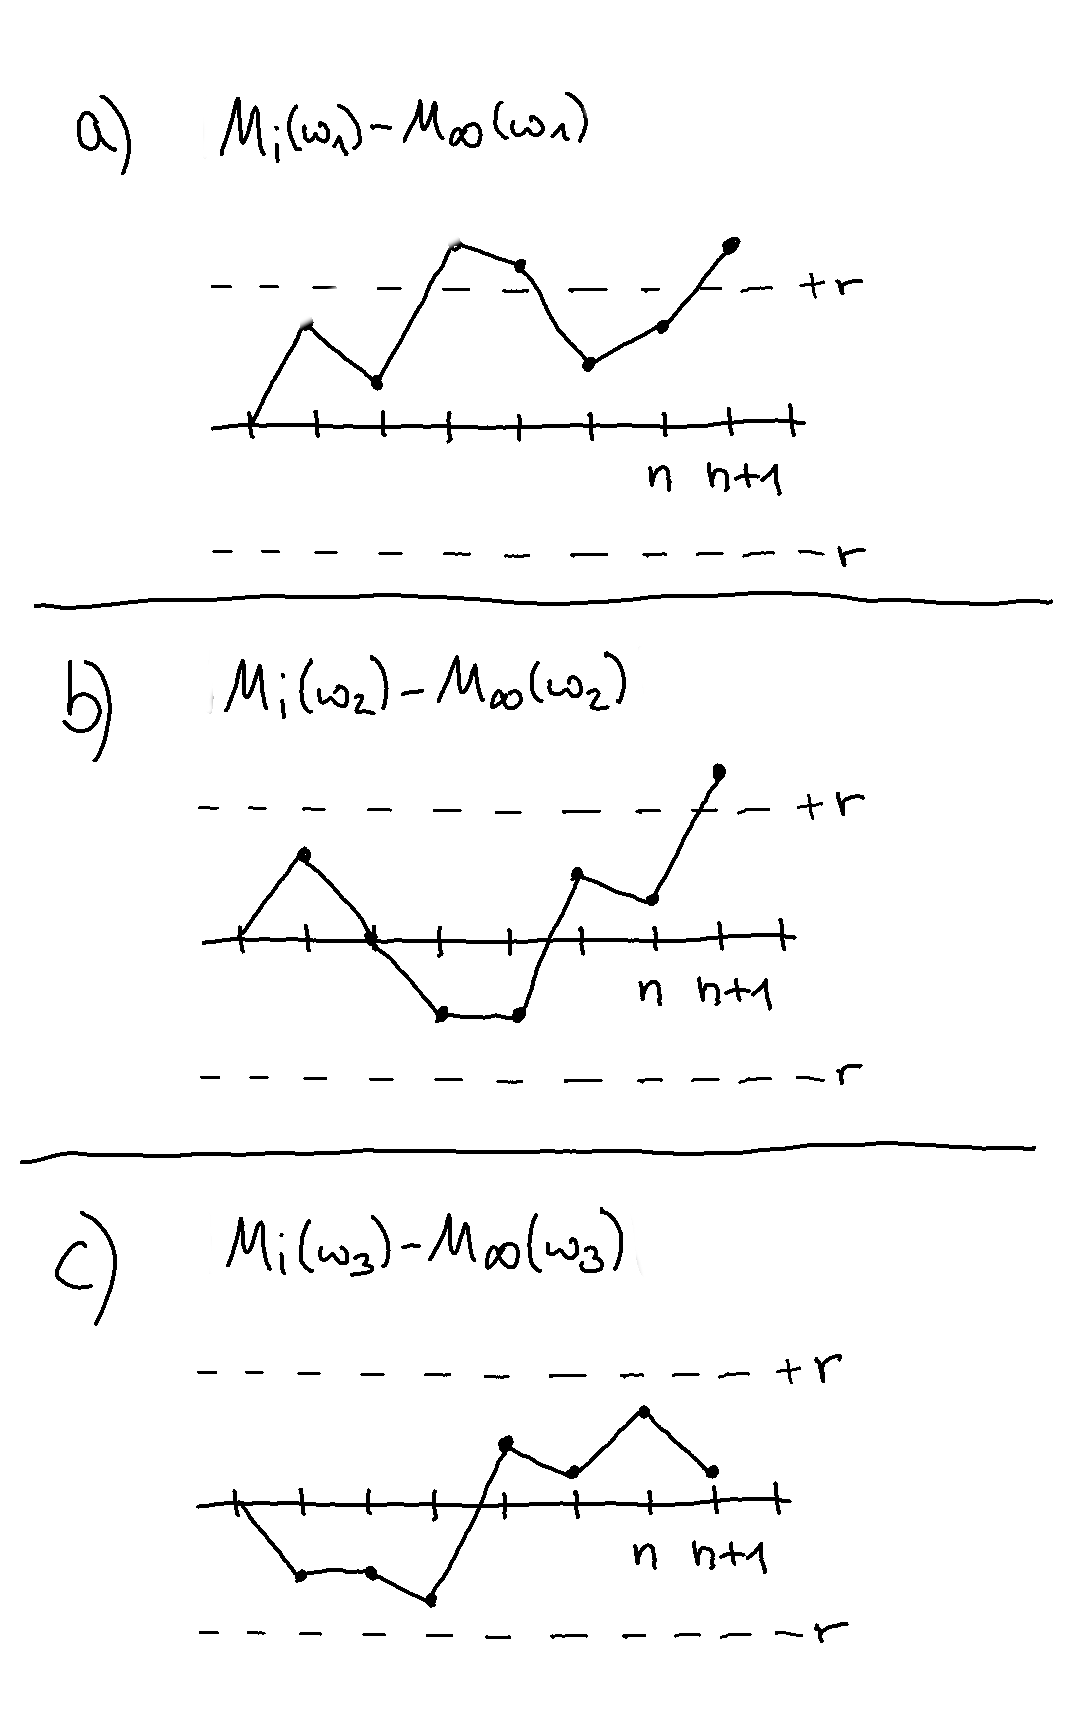
\includegraphics[width=0.65\textwidth]{\pathPrefix pics/SketchUE1.png}
		\begin{enumerate}[label=Fall \alph{*})]
			\item \qquad $\omega_1 \in A_n \quad \rightarrow\quad \omega_1 \in A_{n+1}$
			\item \qquad $\omega_2 \not\in A_n \quad \rightarrow \quad \omega_2 \in A_{n+1}$
			\item \qquad $\omega_3 \not\in A_n \quad \rightarrow \quad \omega_3 \not\in A_{n+1}$
		\end{enumerate}
		$\omega \in A_n \quad \rightarrow \quad \omega \not\in A_{n+1} \quad$ nicht möglich $\implies A_n \subset A_{n+1} \quad\forall n\in\N$
		\label{AbbUEProzess}
	\end{center}
\end{figure}

\begin{proof}[Beweis vom Professor]\enter
	$|M_n|$ ist Submartingal. Aus 4.2 folgt:
	\begin{align*}
		\exists M_\infty\in L_1:\P\left(\limn M_n=M_\infty\right)=1
	\end{align*}
	Mit Fatou kann man zeigen:
	\begin{align*}
		\E\Big[|M_\infty|^p\Big]
		&=\E\left[\limn |M_n|^p\right]
		\overset{\text{Fatou}}{\leq}
		\liminf\limits_{n\to\infty}\E\Big[|M_n|^p\Big]\leq B<\infty\\
		&\implies M_\infty\in L_p
	\end{align*}
	Jetzt nutzen wir majorierte Konvergenz:
	\begin{align*}
		\big|M_n-M_\infty\big|^p
		&\leq
		2^{p-1}\cdot\Big(|M_n|^p+|M_\infty|^p\Big)\\
		&\leq 2^{p-1}\cdot\Bigg(\left(\sup\limits_{n\in\N_0}|M_n|\right)^p+\underbrace{|M_\infty|^p}_{\text{integrierbar}}\Bigg)
	\end{align*}
	Mit Doobs $L_p$-Ungleichung folgt:
	\begin{align*}
		\left\Vert\sup\limits_{0\leq n\leq N}|M_n|\right\Vert_p
		&\leq \frac{p}{p-1}\cdot\Vert M_n\Vert_p\leq B\\
		\implies
		\left\Vert\sup\limits_{0\leq n\leq N}|M_n|\right\Vert_p
		&\leq B<\infty
	\end{align*}
	d.h. $|M_n-M_\infty|^p$ ist integrierbare obere Schranke. Folglich:
	\begin{align*}
		\limn\E\left[|M_n-M_\infty|^p\right]	
		\overset{\text{domKonv}}=
		\E\left[\limn|M_n-M_\infty|^p\right]=0
	\end{align*}
\end{proof}


% This work is licensed under the Creative Commons
% Attribution-NonCommercial-ShareAlike 4.0 International License. To view a copy
% of this license, visit http://creativecommons.org/licenses/by-nc-sa/4.0/ or
% send a letter to Creative Commons, PO Box 1866, Mountain View, CA 94042, USA.

\section{Aufgabenblatt 4}
\subsection{Aufgabe 4.1 (Monotonie der klassischen Aussagenlogik)}
Seien $G$ aussagenlogische Formel und seien $\F$ und $\F'$
Mengen aussagenlogischer Formeln. 
Dann gilt:
\begin{align*}
	\big(\F\models G\und \F\subseteq\F'\big)\implies\F'\models\F
\end{align*}
Erinnerung:
\begin{align*}
	\F'\models G:\Longleftrightarrow\big(\forall I:I\models\F'\implies I\models G\big)
\end{align*}

\begin{proof}
	Sei also $I$ beliebige Interpretation mit $I\models\F'$. 
	Dann gilt nach Definition
	\begin{align*}
		\forall F'\in\F':I\models F'
	\end{align*}
	Da $\F\stackrel{\text{Vor}}{\subseteq}\F'$ folgt 
	\begin{align*}
		\forall F\in\F:I\models F
	\end{align*}
	Aus der Voraussetzung $\F\models G$ folgt nun $I\models G$. 
	Da die Interpretation $I$ beliebig war, folgt die Behauptung $\F'\models G$. 
\end{proof}

\subsection{Aufgabe 4.2  (Wissenswertes über Nessie)}
\subsubsection{Aufgabe 4.2 (a)}
\begin{align*}
	F_1 &=(m \to\neg s)\\
	F_2 &=(\neg m\to (s\wedge t))\\
	F_3&=((\neg s\vee t)\to d)\\
	F_4&=(d\to a)
\end{align*}

\subsubsection{Aufgabe 4.2 (b)}
Wissen über Nessie ist $\F:=\lbrace F_1,\ldots, F_4\rbrace$.
``Folgt daraus, dass Nessie ein Märchenwesen ist?'', d. h.
Frage: Gilt $\F\models m$?

\begin{lösung}
	Man könnte an dieser Stelle \textit{Resolution} verwenden, aber es geht auch naiv. 
	Betrachte die Interpretation $I_1$ mit\\
	$m^{I_1}=\top,~s^{I_1}=\bot,~d^{I_1}=\top,~a^{I_1}=\top$ und $t^{I_1}$ beliebig\\ und die Interpretation $I_2$ mit\\
	$m^{I_2}=\bot,~s^{I_2}=\bot,~t^{I_2}=\top, d^{I_2}=\top,a^{I_2}=\top$\\
	Dann gilt $I_1\models\F$ und $I_2\models\F$ aber $I_1\models m$ und $I_2\not\models m$. 
	Also folgt $F\not\models m$ und $\F\not\models\neg m$.
	Man kann also nichts folgern.
\end{lösung}

\subsection{Aufgabe 4.3 (Logische Äquivalenzen)}
Beachte zunächst
\begin{align*}
	G\equiv F &\stackrel{\text{Def}}{\Longleftrightarrow}
	\Big(\forall I:I\models F\gdw I\models G\Big)\\
	\overset{\text{Def}}&{\Longleftrightarrow}
	\Big(\forall I:G^I=\top\gdw F^I=\top\Big)\\
	&\Longleftrightarrow\forall I:F^I=G^I
\end{align*}

Sei also $I$ eine beliebige Interpretation im Folgenden.

\subsubsection{Aufgabe 4.3 (a)}
\begin{align*}
	[(F\vee F)]^I=F^I\vee^\ast F^I\stackeq{\text{Tab}} F^I
\end{align*}
\begin{tabular}{c||c}
	$F^I$ & $F^I\vee^\ast F^I$\\ \hline
	$\top$ & $\top$\\
	$\bot$ & $\bot$
\end{tabular}

\subsubsection{Aufgabe 4.3 (b)}
\begin{align*}
	[\neg(F\wedge G)]^I=\neg^\ast\left(F^I\wedge^\ast G^I\right)\stackeq{\text{Tab}}
	\left(\neg^\ast F^I\vee^\ast\neg^\ast G^I\right)=\big[(\neg F\vee\neg G)\big]^I
\end{align*}

\begin{tabular}{c|c||c|c}
	$F^I$ & $G^I$ & $\neg^\ast(F^I\wedge^\ast G^I)$ & $(\neg^\ast F^I\vee^\ast\neg^\ast G^I)$\\ \hline
	$\top$ & $\top$ & $\bot$ & $\bot$\\
	$\top$ & $\bot$ & $\top$ & $\top$\\
	$\bot$ & $\top$ & $\top$ & $\top$\\
	$\bot$ & $\bot$ & $\top$ & $\top$
\end{tabular}

\subsubsection{Aufgabe 4.3 (c)}
Analog zu (a) und (b).
%\begin{align*}
%[(F\to G)]^I=\left(F^I\to^\ast G^I\right)\stackeq{\text{Tab}}
%\left( F^I\to^\ast\neg^\ast G^I\right)=\big[(\neg F\vee\neg G)\big]
%\end{align*}

\subsubsection{Aufgabe 4.3 (d)}
Analog zu (a) und (b).

\subsubsection{Aufgabe 4.3 (e)}
Analog zu (a) und (b).

\subsubsection{Aufgabe 4.3 (f)}
Analog zu (a) und (b).

\subsubsection{Aufgabe 4.3 (g)}
Analog zu (a) und (b).

\subsection{Aufgabe 4.4 (Das vollständige Junktorensystem \texorpdfstring{$\lbrace\neg, \vee\rbrace$}{lbrace neg,vee rbrace})}
Zeigen Sie: Es gibt zu jeder aussagenlogischen Formel (mit was auch immer für ein-und zweistelligen Junktoren aus dem Reservoir der 4 bzw. 16 möglichen Junktoren) eine
semantisch äquivalente Formel, welche nur die Junktoren $\neg$ und $\vee$ enthält.

\begin{lösung}
	Sei $\mathcal{R}=\lbrace p_1,p_2,\ldots\rbrace$ eine Menge von aussagenlogischen Variablen, 
	$J_1:=\lbrace J_1^1,\ldots,J_1^4\rbrace$ die Menge der einstelligen Junktoren und $J_2:=\lbrace J_2^1,\ldots,J_2^{16}\rbrace$ die Menge der zweistelligen Junktoren. 
	(Es gibt nach Vorlesung genau 4 einstellige und 16 zweistellige Junktoren). 
	Es müssen also zunächst folgende 16 + 4 Ersetzungsrelegung bzw. semantische Äquivalenzen gezeigt werden (analog zu Aufgabe 4.3):
	\begin{enumerate}
		\item $J_1^1 A\equiv\neg A$
		\item $J_1^2 A\equiv\neg\neg A$
		\item $J_1^3 A\equiv A\vee\neg A$
		\item $J_1^4 A\equiv\neg(A\vee\neg A)$
	\end{enumerate}
	und
	\begin{enumerate}
		\item $A J_2^1 B\equiv A\vee B$
		\item $A J_2^2 B=A\wedge B\equiv\neg(\neg A\vee\neg B)$
		\item $A J_2^3 B=A\to B\equiv\neg A\vee B$
		\item $\ldots$
	\end{enumerate}
	Nun können wir eine rekursive Funktion auf der Menge der Formeln über den 16+4 Junktoren definieren.
	Diese konkret aufzuschreiben ist etwas awkward und wird hier nicht gemacht.
\end{lösung}

\textbf{Mitschrift aus der Übung:}
\begin{lösung}
	Leite für jeden Junktor aus der Wahrheitswertetabelle eine äquivalente Formel und daraus dann eine Ersetzungsregel ab. 
	Dabei nutzen wir die de'Morgansche Regel:
	\begin{align*}
		(\varphi_1\wedge\varphi_2)\equiv\neg(\neg\varphi_1\vee\neg\varphi_2)
	\end{align*}
	Daraus erhält man die Ersetzungsregel
	\begin{align}\label{4.4Ersetzungsregel}
		\frac{(\varphi_1\wedge\varphi_2)}{\neg(\neg\varphi_1\vee\neg\varphi_2)}
	\end{align}
	Hier am Beispiel der Implikation:\\
	\begin{tabular}{c|c||c}
		$\varphi_1^I$ & $\varphi_2^I$ & $\varphi_1^I\to^\ast\varphi_2^I$ \\ \hline
		$\top$ & $\top$ & $\top$\\
		$\top$ & $\bot$ & $\bot$\\
		$\bot$ & $\top$ & $\top$\\
		$\bot$ & $\bot$ & $\top$
	\end{tabular}

	\begin{align*}
		(\varphi_1\to\varphi_2)
		&\equiv (\varphi_1\wedge\varphi_2)\vee(\neg\varphi_1\wedge\varphi_2)\vee(\neg\varphi_1\wedge\neg\varphi_2)\\
		\overset{\eqref{4.4Ersetzungsregel}}&{\equiv}
		\neg(\neg\varphi_1\vee\neg\varphi_2)\vee\neg(\neg\neg\varphi_1\vee\varphi_2)\vee\neg(\neg\neg\varphi_1\vee\neg\neg\varphi_2)\\
		&\equiv(\neg\varphi_1\vee\varphi_2)
	\end{align*}
	Somit erhält man die Ersetzungsregel
	\begin{align*}
		\frac{(\varphi_1\to\varphi_2)}{(\neg\varphi_1\vee\varphi_2)}
	\end{align*}
	Erhalte somit alle 16 + 4 Ersetzungsregel erschöpfend auf die Formel an (d.h. bis keine Ersetzungsregel mehr anwendbar ist). 
	Damit erhält man nach endlich vielen Schritten eine semantisch äquivalente Formel, welche nur noch $\neg$ und $\vee$ enthält.
\end{lösung}

\subsection{Aufgabe 4.5 (Positionen und Ersetzungen in Formeln)}
\subsubsection{Aufgabe 4.5 (a)}
\begin{tikzpicture}[node distance=5em]
	\tikzstyle{every state}=[shape=circle,draw=black]
	\node[state] (1) {$\neg:\Lambda$};
	\node[state] (2) [below = of 1] {$\wedge:1$};
	\node[state] (3) [below left = of 2] {$p:11$};
	\node[state] (4) [below right = of 2] {$\vee:12$};
	\node[state] (5) [below left = of 4] {$q:121$};
	\node[state] (6) [below right = of 4] {$\neg:122$};
	\node[state] (7) [below of =6] {$p:1221$};
	\path 	(2) edge [, -] node {} (1)
   	   		(3) edge [, -] node {} (2)
		 	(4) edge [, -] node {} (2)
	  		(5) edge [, -] node {} (4)
	 		(6) edge [, -] node {} (4)
	  		(7) edge [, -] node {} (6)
	;	
\end{tikzpicture}

\begin{align*}
	\mathcal{P}_F=\lbrace\Lambda,1,11,12,121,122,1221\rbrace
\end{align*}
Formal:
\begin{align*}
	\pos(\neg(p\wedge(q\vee\neg p)))
	\overset{2.}&=
	\lbrace\Lambda\rbrace\cup\lbrace 1\pi:\pi\in\pos((p\wedge(q\vee\neg p)))\rbrace\\
	&=\lbrace\Lambda,1\Lambda,11\Lambda,12\Lambda,121\Lambda,122\Lambda,1221\Lambda\rbrace\\
	\pos((p\wedge(q\vee\neg p)))
	\overset{3}&=
	\lbrace\Lambda\rbrace\cup\lbrace 1\pi_1:\pi_1\in\pos(p)\rbrace\cup\lbrace 2\pi_2:\pi_2\in\pos((q\vee\neg p))\rbrace\\
	&=\lbrace\Lambda,1\Lambda,2\Lambda,21\Lambda,22\Lambda,221\Lambda\rbrace\\
	\pos(p)&\stackeq{1.}\lbrace\Lambda\rbrace\cup\emptyset=\lbrace\Lambda\rbrace\\
	\pos((q\vee\neg p))&\stackeq{3.}\lbrace\Lambda\rbrace\cup\lbrace1\pi_1:\pi_1\in\pos(q)\rbrace\cup\lbrace 2\pi_2:\pi_2\in\pos(\neg p)\rbrace\\
	&=\lbrace\Lambda,1\Lambda,2\Lambda,21\Lambda\rbrace\\
	\pos(q)&\stackeq{1.}\lbrace\Lambda\rbrace\cup\emptyset=\lbrace\Lambda\rbrace\\
	\pos(\neg p)&\stackeq{2.}\lbrace\Lambda\rbrace\cup\lbrace 1\pi:\pi\in\pos(p)\rbrace=\Lambda,1\Lambda\rbrace
\end{align*}

\subsubsection{Aufgabe 4.5 (b)}
\begin{tikzpicture}[node distance=5em]
	\tikzstyle{every state}=[shape=circle,draw=black]
	\node[state] (1) {$\neg:\Lambda$};
	\node[state] (2) [below = of 1] {$\neg:1$};
	\node[state] (3) [below = of 2] {$\wedge:11$};
	\node[state] (4) [left = of 3] {$\vee:111$};
	\node[state] (5) [below left = of 4] {$p:1111$};
	\node[state] (6) [below right = of 4] {$q:1112$};
	\node[state] (7) [right = of 3] {$\vee:112$};
	\node[state] (8) [below left = of 7] {$q:1121$};
	\node[state] (9) [below right = of 7] {$\neg:1122$};
	\node[state] (10) [below = of 9] {$p:11221$};
	\path 	(2) edge [, -] node {} (1)
      		(3) edge [, -] node {} (2)
	  		(4) edge [, -] node {} (3)
	  		(5) edge [, -] node {} (4)
	  		(6) edge [, -] node {} (4)
	  		(7) edge [, -] node {} (3)
	  		(8) edge [, -] node {} (7)
	  		(9) edge [, -] node {} (7)
	  		(10) edge [, -] node {} (9)
	;	
\end{tikzpicture}

\begin{align*}
	G\lceil 1122\Lambda\rceil
	&=\Big[\neg\neg((p\vee q)\wedge(q\vee\neg p))\Big]\lceil 1122\Lambda\rceil\\
	&\stackeq{\text{2.}}
	\Big[\neg((p\vee q)\wedge(q\vee\neg p))\Big]\lceil 122\Lambda\rceil\\
	&\stackeq{\text{2.}}
	\Big[((p\vee q)\wedge(q\vee\neg p))\Big] \lceil 22\Lambda\rceil\\
	&\stackeq{\text{3.}}
	\Big[(q\vee\neg p)\Big]\lceil 2\Lambda\rceil\\
	&\stackeq{\text{3.}}
	[\neg p]\lceil\Lambda\rceil\\
	&\stackeq{\text{1.}}[\neg p]=\neg p
\end{align*}

\subsubsection{Aufgabe 4.5 (c)}
\begin{tikzpicture}[node distance=3em]
	\tikzstyle{every state}=[shape=circle,draw=black]
	\node[state] (1) {$\neg:\Lambda$};
	\node[state] (2) [below = of 1] {$\wedge:1$};
	\node[state] (3) [below left = of 2] {$\neg:11$};
	\node[state] (4) [below left = of 3] {$\vee:111$};
	\node[state] (5) [below left = of 4] {$p:1111$};
	\node[state] (6) [below right= of 4] {$q:1112$};
	\node[state] (7) [below right = of 2] {$\neg:12$};
	\node[state] (8) [below right = of 7] {$\vee:121$};
	\node[state] (9) [below left = of 8] {$q:1211$};
	\node[state] (10) [below right = of 8] {$\neg:1212$};
	\node[state] (11) [below = of 10] {$p:12121$};
	\path 	(2) edge [, -] node {} (1)
   		   	(3) edge [, -] node {} (2)
	  		(4) edge [, -] node {} (3)
	  		(5) edge [, -] node {} (4)
	  		(6) edge [, -] node {} (4)
	  		(7) edge [, -] node {} (2)
	  		(8) edge [, -] node {} (7)
	  		(9) edge [, -] node {} (8)
	  		(10) edge [, -] node {} (8)
	  		(11) edge [, -] node {} (10)
		;	
\end{tikzpicture}

\begin{align*}
	H\Big\lceil 121\Lambda\mapsto(\neg p\to q)\Big\rceil
	&=
	\Big[\neg(\neg(p\vee q)\wedge\neg(q\vee\neg p))\Big]\Big\lceil 121\Lambda\mapsto(\neg p\to q)\Big\rceil\\
	&\stackeq{\text{2.}}
	\neg\Big[(\neg(p\vee q)\wedge\neg(q\vee\neg p))\Big]\Big\lceil 21\Lambda\mapsto(\neg p\to q)\Big\rceil\\
	&\stackeq{\text{4.}}
	\neg\Big(\neg(p\vee q)\wedge\Big[\neg(q\vee\neg p)\Big]\Big\lceil 1\Lambda\mapsto(\neg p\to q)\Big\rceil\Big)\\
	&\stackeq{\text{2.}}
	\neg\Big(\neg(p\vee q)\wedge\neg\Big[(q\vee\neg p)\Big]\Big\lceil\Lambda\mapsto(\neg p\to q)\Big\rceil\Big)\\
	&\stackeq{\text{1.}}
	\neg\Big(\neg(p\vee q)\wedge\neg(\neg p\to q)\Big)
\end{align*}
Zur semantischen Äquivalenz: Das Ersetzungstheorem (Satz 3.23) ist nicht anwendbar, da 
\begin{align*}
	(q\vee\neg p)\not\equiv(\neg p\to q)
\end{align*}
Tatsächlich gilt
\begin{align*}
	H\not\equiv H\lceil 121\mapsto(\neg p\to q)\rceil
\end{align*}
Betrachte die Interpretation $I$ mit $p^I=q^I=\bot$.

\subsection{Aufgabe 4.6 (Formelersetzungen)}
\subsubsection{Aufgabe 4.6 (a)}
Die Aussage gilt nicht, denn betrachte folgendes Gegenbeispiel:\\
$F=(p\wedge p)=p\vee G$ mit $\pi=1$ und $H=\neg p$. 
Dann sind $F,G,H$ erfüllbar aber \\
$F\lceil\pi\to H\rceil=(p\vee\neg p)$ ist unerfüllbar.\\
Also: Obwohl die Formeln $F,G,H$ unabhängig voneinander erfüllbar sind, können in $H$ Variablen verwendet werden, die auch an anderer Stelle in $F$ vorkommen.

\subsubsection{Aufgabe 4.6 (b)}
Die Aussage stimmt, denn:\\
Durch scharfes Hinsehen (oder Wahrheitswertetabelle) sieht man (aufgrund der Unerfüllbarkeit von $G$)
\begin{align*}
	G\equiv((H\wedge G)\wedge(H\vee G))
\end{align*}
Nach dem Ersetzungstheorem (Satz 3.23) folgt damit die Behauptung, da in $F$ eine Teilformel durch eine semantisch äquivalente Formel ersetzt wird.

\subsubsection{Aufgabe 4.6 (c)}
Die Aussage stimmt nicht. Betrachte\\
$F=\neg p,\pi=1\Lambda,G=p,H=(p\vee q)$, offensichtlich ist $G\to H$ eine Tautologie, aber $F\to F\lceil\pi\mapsto H\rceil=\neg p\to\neg(p\vee q)$ nicht allgemeingültig. Denn $p^I=\bot$, $q^I=\top$)

%$G=H=p\wedge\neg p$ und $F=\neg H$ mit $\pi=\Lambda$. Dann ist $H\to G$ allgemeingültig, aber
%$F\to \underbrace{F\lceil\pi\to G\rceil}_{=H}$ ist unerfüllbar, denn $F$ ist allgemeingültig und $H$ unerfüllbar.\\


% This work is licensed under the Creative Commons
% Attribution-NonCommercial-ShareAlike 4.0 International License. To view a copy
% of this license, visit http://creativecommons.org/licenses/by-nc-sa/4.0/ or
% send a letter to Creative Commons, PO Box 1866, Mountain View, CA 94042, USA.
% vim: set noexpandtab:

\section{Aufgabenblatt 5}
\subsection{Aufgabe 5.1}
Sei $K=(a,a+h)$ mit $a\in\R$ und $h>0$ ein offenes Intervall.

\subsubsection{Aufgabe 5.1 (a)}
Es gilt für alle $v\in P_k(K)$ und $0\leq m\leq l$ sowie $p,q\in[1,\infty]$ die inverse Ungleichung
\begin{align*}
	|v|_{l,p,K}\leq c\cdot h^{m-l+\left(\frac{1}{p}-\frac{1}{q}\right)}\cdot|v|_{m,q,K}
\end{align*}
wobei $C$ eine Konstante ist, die nicht von $K$ abhängt (und damit insbesondere auch nicht von $h$).

\begin{proof}
	%Nutze Transformation auf Referenzelement $\hat{K}=(0,1)$, also
	%\begin{align*}
		%f:\R\to\R,\qquad x\mapsto h\cdot x+a
	%\end{align*}
	In Aufgabe 4.5 haben wir gezeigt für $\hat{K}=(0,1)$:
	\begin{align*}
		|\hat{v}|_{m,p,\hat{K}}\leq h^m\cdot\left(\frac{1}{h}\right)^{\frac{1}{p}}\cdot|v|_{m,p,K}
	\end{align*}
	Damit folgt:
	\begin{align*}
		|v|_{l,p,K}
		&=\underbrace{h^{-l}\cdot\left(\frac{1}{h}\right)^{-\frac{1}{p}}}_{=h^{-l+\frac{1}{p}}}\cdot\underbrace{|\hat{v}|_{l,p,\hat{K}}}_{\stackrel{l\geq m}{\leq}\Vert \hat{v}^{(m)}\Vert_{l-m,p,\hat{K}}}
	\end{align*}
	Jetzt nutzen wir die Äquivalenz der Normen auf dem endlich dimensionalem Raum $P_k(\hat{K})$:
	\begin{align*}
		\Vert \hat{v}^{(m)}\Vert_{l-m,p,\hat{K}}
		&\leq
		c\cdot\underbrace{\Vert\hat{v}^{(m)}\Vert_{0,q,\hat{K}}}_{=|\hat{v}|_{m,q,\hat{K}}}
	\end{align*}
	wobei $c$ unabhängig von $h(K)$ ist wegen des Referenzelements $\hat{K}$. Folglich gilt:
	\begin{align*}
		|v|_{l,p,K}
		&\leq
		c\cdot h^{-l+\frac{1}{p}}\cdot\underbrace{|\hat{v}|_{m,q,\hat{K}}}_{\stackeq{\text{Aufg. 4.5}}h^{k-\frac{1}{q}}\cdot|v|_{m,q,\hat{K}}}
		=c\cdot h^{m-l+\left(\frac{1}{p}-\frac{1}{q}\right)}\cdot|v|_{m,q,K}
	\end{align*}
	%Es gilt
	%\begin{align*}
		%\min\limits_{p\in P_k}\big\Vert\hat{v}+p\big\Vert_{0,p,\hat{K}}\leq c\cdot|\hat{v}|_{k+1,p,\hat{K}}
	%\end{align*}
\end{proof}

\begin{bemerkung}
	Falls $v$ eine Funktion auf einen Finiten-Elemente-Raum (also endlich dimensional) ist, das Element $(K,V,\Sigma)$ von der Triangulierung affin äquivalent zum Referenzelement $(\hat{K},\hat{V},\hat{\Sigma})$ ist, dann gilt:
	\begin{align*}
		\Vert v\Vert_{l,p,K}\leq c\cdot h_K^m\cdot\rho_k^{-l}\cdot\meas(K)^{\frac{1}{p}-\frac{1}{q}}\cdot\Vert v\Vert_{m,q,K}
	\end{align*}
	Falls $n$ die Dimension notiert, dann gilt:
	\begin{align*}
		c\cdot \rho_k^n&\leq\meas(K)\leq c\cdot h_k^n\\
		\frac{h_k}{\rho_k}&\leq c\qquad\text{(form-regulär)}\\
		\implies\Vert v\Vert_{l,p,K}&\leq c\cdot h_K^{m-l+n\cdot\left(\frac{1}{p}-\frac{1}{q}\right)}\cdot\Vert v\Vert_{m,q,K}\\
		\Vert v\Vert_{l,p,K}&=\sum\limits_{i=}^{m+1}\big| v^{(i)}\big|_{0,p,K}+\big\Vert v^{(m)}\big\Vert_{l-m,p,K}
	\end{align*}
	Rest der Lösung steht online.
	% login: PDENM18, PW: weak
\end{bemerkung}

$V_h\subseteq V$ ist konform mit $V\subseteq H^1(\Omega)\hookrightarrow C(\Omega)$\\
$V_h\not\subseteq V$ ist nichtkonform.

\subsubsection{Aufgabe 5.1 (b)}
Wie muss die rechte Seite angepasst werden, wenn die volle $W^{l,p}$-Norm in ähnlicher Weise abgeschätzt werden soll?

\begin{lösung}
	%TODO
\end{lösung}

\subsection{Aufgabe 5.2}
Im Rahmen nichtkonformer Finite Elemente soll die folgende Verallgemeinerung des Dualitätsarguments von Aubin-Nitsche untersucht werden.\\
Sei $H$ ein Hilbertraum mit Norm $\Vert\cdot\Vert_H$ und Skalarprodukt $(\cdot,\cdot)$. 
Ferner sei $V_h\subseteq H$ abgeschlossen mit Norm $\Vert\cdot\Vert_h$ und $V$ ein Hilbertraum, welcher stetig in $H$ eingebettet ist $(V\hookrightarrow H$). 
Die auf $V+V_h$ definierte und stetige Bilinearform $a_h$ stimme auf $V$ mit $a$ überein. 
Dann gilt:
\begin{align*}
	\Vert u-u_h\Vert_H\leq\sup\limits_{g\in H\setminus\lbrace0\rbrace}\frac{1}{\Vert g\Vert_H}\cdot\Big( &M\cdot\Vert u-u_h\Vert_h\cdot\Vert\varphi_g-\varphi_{g,h}\Vert_h\\
	&+\big|a_h(u-u_h,\varphi_g)-(u-u_h,g)\big|\\
	&+\big|a_h(u,\varphi_g-\varphi_{g,h})-(f,\varphi_g-\varphi_{g,h})\big|\Big)
\end{align*}
wobei zu $g\in H$ die Funktionen $\varphi_g\in V$ und $\varphi_{g,h}\in V_h$ als Lösungen von
\begin{align*}
	a(w,\varphi_g)=(w,g)\quad\forall w\in V\qquad\text{bzw.}\qquad a_h(w_h,\varphi_{g,h})=(w_h,g)\quad\forall w_h\in V_h
\end{align*}
definiert sind.

\begin{proof}
	Auf $V\times V$ gilt $a=a_h$
	\begin{align*}
		a_h:(V+V_h)\times(V+V_h),\qquad
		a(u,v)&=\int\limits_\Omega\nabla u\cdot\nabla v\d x\\
		a_h(u,v)&=\sum\limits_{K}\int\limits_K\nabla u\cdot\nabla v\d x
	\end{align*}
	Setze $\varphi_h:=\varphi_{g,h}$. Dann gilt:
	\begin{align*}
		(u-u_h,g)&=a(\underbrace{u}_{\in V},\underbrace{\varphi_g}_{\in V})-a_h(u_h,\varphi_h)\\
		&=a_h(u,\varphi_g)-a_h(u_h,\varphi_h)\\
		&=a_h(u,\varphi_g\underbrace{-\varphi_h)+a_h(u,\varphi_h)}_{=0}-a_h(u_h,\varphi_h)\\
		&{} \quad-\underbrace{a_h(u_h,\varphi_g-\varphi_h)+a_h(u_h,\varphi_g-\varphi_h)}_{=0}\\
		&=a_h(u-u_h,\varphi_g-\varphi_h)+\underbrace{a_h(u-u_h,\varphi_h)}_{(1)}+\underbrace{a_h(u_h,u_g-\varphi_h)}_{(2)}
	\end{align*}
	%TODO hier fehlt was
	und außerdem
	\begin{align*}
		a_h(u,\varphi_g-\varphi_h)-(f,\varphi_g-\varphi_h)
		&=\underbrace{a_h(u,\varphi_g)-(f,\varphi_g)}_{=0, \text{weak solution}}-a_h(u,\varphi_h)+\underbrace{(f,\varphi_h)}_{\stackeq{\text{Def }u_h}a_h(u_h,\varphi_h)}\\
		&=-a_h(u-u_h,\varphi_h) = (1)
	\end{align*}
	und außerdem %Wortwiederholung als Ausdruck von Langeweile
	\begin{align*}
		a_h(u-u_h,\varphi_g)-(u-u_h,g)
		&=\underbrace{a(u,\varphi_g)-(u,g)}_{=0}-a_h(u_h,\varphi_g)+\underbrace{(u_h,g)}_{=a_h(u_h,\varphi_h)}\\
		&=-a_h(u_h,\varphi_g-\varphi_h) = -(2)
	\end{align*}
	und außerdem %Wortwiederholung als Ausdruck von Langeweile
	\begin{align*}
		\Vert u-u_h\Vert
		&=\sup\limits_{g\in H\setminus\lbrace0\rbrace}\frac{(u-u_h,g)}{\Vert g\Vert_H}
	\end{align*}
	Damit folgt mit der Stetigkeit von $a_h$ und dem Betrag auf der rechten Seite die Behauptung.
\end{proof}

\subsection{Aufgabe 5.3}
Sei $\Omega$ ein konvexes Polyeder. Beweisen Sie für die Diskretisierung der Poisson-Gleichung
\begin{align*}
	\left\lbrace\begin{array}{rl}
		-\Delta u=f &\text{ in }\Omega\\
		u|_{\partial\Omega}=0
	\end{array}\right.\mit f\in L^2(\Omega)
\end{align*}
mit Crouzeix-Raviart-Elementen über einer regulären Zerlegung von $\Omega$ die \\$L^2$-Fehlerabschätzung
\begin{align*}
	\Vert u-u_h\Vert_0\leq c\cdot h^2\cdot\Vert u\Vert_2
\end{align*}

\begin{proof}
	$V=H_0^1(\Omega)$, $H=L^2$, $V_h\not\subseteq V$
	\begin{align*}
		a(v,w)&=\int\limits_\Omega\nabla v\cdot\nabla w\d x\\
		a_h(v,w)&=\sum\limits_K\int\limits_K\nabla v\cdot\nabla w\d x
	\end{align*}

	\underline{Teilschritt (a):}\\
	Das Dualitätsargument von Aubin-Nitsche ist anwendbar (klar).\nl
	\underline{Teilschritt (b):}\\
	Aus der Vorlesung ist bekannt:
	\begin{align*}
		\Vert u-u_h\Vert_h\leq c\cdot h\cdot\Vert u\Vert_2
	\end{align*}
	Bei der Abschätzung von $\Vert\varphi_g-\varphi_{g,h}\Vert$ hilft, dass $\varphi_g-\varphi_{g,h}$ als Diskretisierungsfehler des Problems 
	$a(w,\varphi)=(w,g)$ angesehen werden kann.\nl
	$\varphi_g$ und $\varphi_{g,h}$ sind auch schwache und diskrete Lösungen der Poisson-Gleichung, aber mit rechter Seite $g$ anstelle von $f$. 
	Folglich kann die Abschätzung aus der Vorlesung benutzt werden und es gilt
	\begin{align*}
		\Vert\varphi_g-\varphi_{g,h}\Vert_h\leq c\cdot h\cdot\Vert\varphi_g\Vert_2
	\end{align*}

	\underline{Teilschritt (c):}\\
	Es ist bekannt:
	\begin{align*}
		\big|L_w(z)\big|:=\Big|a_h(w,z)-(\hat{f},z)\Big|\leq c\cdot h\cdot\Vert w\Vert_2\cdot\Vert z\Vert_h\qquad\forall z\in V_h+v,\forall w\in H^2
	\end{align*}
	und $w$ erfüllt die Gleichung $-\Delta w = \hat{f}$.%f_{snake}%\~{f}$
	Dann folgt:
	\begin{align*}
		\underbrace{\big|a_h(u-u_h,\varphi_g)-(u-u_h,g)\big|}_{=|L_{\varphi_g}(u-u_h)|} &\leq Ch \|\varphi_g\|_2\underbrace{\|u-u_h\|_h}_{Ch\|u\|_2}\\
		&\leq Ch^2 \|u\|_2\|\varphi_g\|_2
	\end{align*}
	und
	\begin{align*}
		\underbrace{\big|a_h(u,\varphi_g-\varphi_{g,h})-(f,\varphi_g-\varphi_{g,h})\big|}_{=|L_{u}(\varphi_g-\varphi_{g,h})|} &\leq Ch \|u\|_2\underbrace{\|\varphi_g - \varphi_{g,h}\|_h}_{Ch\|\varphi_g\|_2} \\
		&\leq Ch^2 \|u\|_2\|\varphi_g\|_2
	\end{align*}

	%TODO vermutlich fehlt hier auch was. Bin dermaßen raus, dass ich das nicht einmal mehr einschätzen kann xD Haha 

	\underline{Teilschritt (d):}
	\begin{align*}
		\Vert u-u_h\Vert_0\leq\sup\limits_{g\in H\setminus\lbrace0\rbrace}\frac{1}{\Vert g\Vert_H}\big\lbrace(\text{MC+CC})~h^2\cdot\Vert u\Vert_2\cdot\underbrace{\Vert\varphi_g\Vert_2}_{C\|g\|_H}\big\rbrace
		\end{align*}
	Aus dem \textit{Regularitäts-Theorem} folgt, da $\Omega$ konvex ist ist:
	\begin{align*}
		\varphi_g\in H^2\qquad\text{und}\qquad\Vert\varphi_g\Vert_2\leq c\cdot\Vert g\Vert_0
	\end{align*}
	$\implies$ 
	\begin{align*}
		\|u-u_h\|_0 \leq C h^2 \|u\|_2.
	\end{align*}
	(Hier wird manchmal die $\|\cdot\|_0$-Norm verwendet. Diese soll anscheinend die $H$-Norm sein.)
\end{proof}

\subsection{Aufgabe 5.4}
	Sei $\Omega$ ein konvexes Polyeder. 
	Es erfülle $w\in H^2(\Omega)\cap H_0^1(\Omega)$ die Poisson-Gleichung $-\Delta w=\hat{f}$. 
	Ferner sei für $z\in V_h+V$
	\begin{align*}
		L_w(z):=a_h(w,z)-(\hat{f},z):=\sum\limits_K\int\limits_K\nabla w\cdot\nabla z\d x-\int\limits_\Omega\hat{f}\cdot z\d x
	\end{align*}
	wobei $V_h$ den Raum der Crouzeix-Raviart-Elemente über einer regulären Zerlegung von $\Omega$ bezeichne und $V=H_0^1(\Omega)$ sein.

\subsubsection{Aufgabe 5.4 (a)}
Es gilt
\begin{align*}
	L_w(z)=\sum\limits_K\sum\limits_{E\in\delta K}\int\limits_E\left(\frac{\partial}{\partial n_K}-\frac{\partial w^I}{\partial n_K}\right)\cdot\left(z-\overline{z(E)}\right)\d s
\end{align*}
Dabei bezeichne $w^I\in V_h\cap C^0(\Omega)$ die stetige, stückweise lineare Interpolierende, die $w$ in den Eckpunkten der Dreiecke interpoliert. 
Auf einer Kante $E$ sei
\begin{align*}
	\overline{z(E)}=\frac{1}{|E|}\cdot\int\limits_E z\d s
\end{align*}
der Integralmittelwert einer Funktion $z\in V_h+V$.

\subsubsection{Aufgabe 5.4 (b)}
Es gilt die Abschätzung
\begin{align*}
	\big|L_w(z)\big|\leq c\cdot h\cdot|w|_2\cdot\Vert z\Vert_h
\end{align*}

\begin{proof}
	Wir nutzen in dem Beweis die Spurungleichung in Kombination mit dem \\ Bramble-Hilbert-Lemma.
	%TODO
\end{proof}

% This work is licensed under the Creative Commons
% Attribution-NonCommercial-ShareAlike 4.0 International License. To view a copy
% of this license, visit http://creativecommons.org/licenses/by-nc-sa/4.0/ or
% send a letter to Creative Commons, PO Box 1866, Mountain View, CA 94042, USA.

\section{Aufgabenblatt 6}
\subsection{Aufgabe 6.1 (Resolutionsableitungen)}
Resolventenbildung: Entferne $A$ aus $C_1$ und $\neg A$ aus $C_2$ und verknüpfe den Rest disjunktiv.\\
Die Auswahl der beiden Klausel für die Resolventenbildung erfolgt mit der \textit{Methode des scharfen Hinsehens}. 
Es ist sinnvoll rückwärts zu denken:
\begin{align*}
	[A,B],[A,\neg B],[\neg A]\Reso[A,A],[\neg A]\Reso[~]
\end{align*}
Eine andere Strategie ist, zu Beginn alle einstelligen Klauseln auszunutzen. 
In Aufgabe 1 (b) kann man in allen Klauseln schon $\neg s$ und $r$ rausstreichen, wegen den Klauseln 4 und 5.

\subsubsection{Aufgabe 6.1}
\begin{align*}
	\begin{array}{rll}
		9 & \Res(2,6,t) & [q,r]\\
		10 & \Res(9, 7,r) & [q]\\
		11 & \Res(10,8,q) & [\neg t]\\
		12 & \Res(11,2, t) & [~]
	\end{array}
\end{align*}

\subsubsection{Aufgabe 6.2}
\begin{align*}
	\begin{array}{rll}
		9 & \Res(4,7,s) & [q,r]\\
		10 & \Res(5,9,r) & [q]\\
		11 & \Res(4,8,s) & [\neg q,\neg q]\\
		13 & \Res(10,11,q) & [~]
	\end{array}
\end{align*}

\subsection{Aufgabe 6.2 (Anwendungen des Resolutionsverfahrens}
Strategie:
\begin{enumerate}
	\item Ersetze $A\to B$ durch $\neg A\vee B$.
	\item Schreibe Formel so um, dass Unerfüllbarkeit zu zeigen ist.
	\item Bringe Formel in KNF mit den bekannten Ersetzungsregeln.
	\item Wende Resolutionsverfahren an (wie Aufgabe 1).
\end{enumerate}

\subsubsection{Aufgabe 6.2 (a)}
Hier schreiben wir direkt die Negation, da wir die Tautologie-Eigenschaft zeigen wollen, indem wir zeigen, dass die Negation unerfüllbar ist.
\begin{align*}
	&\neg((((p\wedge q)\to r)\wedge\neg r)\to(p\to(q\to r)))\\
	&\equiv
	\neg(\neg((\neg(p\wedge q)\vee r)\wedge\neg r)\vee(\neg p\vee(\neg q\vee r)))\\
	&\equiv
	\langle[\neg(\neg((\neg(p\wedge q)\vee r)\wedge\neg r)\vee(\neg p\vee(\neg q\vee r)))]\rangle\\
	&\equiv
	\langle[\neg\neg((\neg(p\wedge q)\vee r)\wedge\neg r)],[\neg(\neg p\vee(\neg q\vee r))]\rangle\\
	&\equiv
	\langle[((\neg(p\wedge q)\vee r)\wedge\neg r)],[\neg(\neg p\vee(\neg q\vee r))]\rangle\\
	&\equiv
	\langle[(\neg(p\wedge q)\vee r)],[\neg r],[\neg(\neg p\vee(\neg q\vee r))]\rangle\\
	&\equiv
	\langle[\neg(p\wedge q), r],[\neg r],[\neg(\neg p\vee(\neg q\vee r))]\rangle\\
	&\equiv
	\langle[\neg p,\neg q, r],[\neg r],[\neg(\neg p\vee(\neg q\vee r))]\rangle\\
	&\equiv
	\langle[\neg p,\neg q, r],[\neg r],[\neg\neg p],[\neg(\neg q\vee r)]\rangle\\
	&\equiv
	\langle[\neg p,\neg q, r],[\neg r],[p],[\neg(\neg q\vee r)]\rangle\\
	&\equiv
	\langle[\neg p,\neg q, r],[\neg r],[p],[\neg\neg q],[\neg r)]\rangle\\
	&\equiv
	\langle[\neg p,\neg q, r],[\neg r],[p],[q],[\neg r]\rangle\\,
	&\begin{array}{rll}
		1 &&[\neg p,\neg q,r]\\
		2 &&[\neg r]\\
		3 &&[p]\\
		4 &&[q]\\
		5 &&[\neg r]\\
		6 & \Res(1,2,r) & [\neg p,\neg q]\\
		7 & \Res(6,3,p) & [\neg q]\\
		8 & \Res(7,4,q) & [~]
	\end{array}
\end{align*}
Damit ist gezeigt, dass die Negation der gegebenen Formel unerfüllbar ist. 
Daher ist die gegebene Formel allgemeingültig (bzw. eine Tautologie).

\subsubsection{Aufgabe 6.2 (b)}
\begin{align*}
	&((\neg r\vee(p\wedge q))\wedge\neg((r\to p)\wedge(r\to q)))\\
	&\equiv
	((\neg r\vee(p\wedge q))\wedge\neg((\neg r\vee p)\wedge(\neg r\vee q)))\\
	&\equiv
	\langle[((\neg r\vee(p\wedge q))\wedge\neg((\neg r\vee p)\wedge(\neg r\vee q)))]\rangle\\
	&\equiv
	\langle[(\neg r\vee(p\wedge q))],[\neg((\neg r\vee p)\wedge(\neg r\vee q))]\rangle\\
	&\equiv
	\langle[\neg r,(p\wedge q)],[\neg((\neg r\vee p)\wedge(\neg r\vee q))]\rangle\\
	&\equiv
	\langle[\neg r, p],[\neg r, q],[\neg((\neg r\vee p)\wedge(\neg r\vee q))]\rangle\\
	&\equiv
	\langle[\neg r, p],[\neg r, q],[\neg(\neg r\vee p),\neg(\neg r\vee q)]\rangle\\
	&\equiv
	\langle[\neg r, p],[\neg r, q],[\neg\neg r,\neg(\neg r\vee q)],[\neg p,\neg(\neg r\vee q)]\rangle\\
	&\equiv
	\langle[\neg r, p],[\neg r, q],[r,\neg(\neg r\vee q)],[\neg p,\neg(\neg r\vee q)]\rangle\\
	&\equiv
	\langle[\neg r, p],[\neg r, q],[r,\neg\neg r],[r,\neg q],[\neg p,\neg(\neg r\vee q)]\rangle\\
	&\equiv
	\langle[\neg r, p],[\neg r, q],[r,\neg\neg r],[r,\neg q],[\neg p,\neg\neg r],[\neg p,\neg q)]\rangle\\
	&\equiv
	\langle[\neg r, p],[\neg r, q],[r,r],[r,\neg q],[\neg p, r],[\neg p,\neg q)]\rangle\\
	&\begin{array}{rll}
		1 &&[\neg r,p]\\
		2 &&[\neg r,q]\\
		3 &&[r,r]\\
		4 &&[\neg r,\neg q]\\
		5 &&[\neg p,r]\\
		6 &&[\neg p,\neg q]\\
		7 & \Res(2,3,r) & [q]\\
		8 & \Res(3,4,r) & [\neg q]\\
		9 & \Res(7,8,q) & [~]
	\end{array}
\end{align*}
Verrechnet, denn das ist erfüllbar mit $p^I=q^I=\top$.

\subsubsection{Aufgabe 6.2 (c)}
Wieder von Beginn an negieren, da wir Unerfüllbarkeit zeigen wollen.
\begin{align*}
	&\neg(((p\to q)\to p)\to p)\\
	&\equiv
	\neg(\neg(\neg(\neg p\vee q)\vee p)\vee p)\\
	&\equiv
	\langle[\neg(\neg(\neg(\neg p\vee q)\vee p)\vee p)]\rangle\\
	&\equiv
	\langle[\neg\neg(\neg(\neg p\vee q)\vee p)], [\neg p]\rangle\\
	&\equiv
	\langle[(\neg(\neg p\vee q)\vee p)], [\neg p]\rangle\\
	&\equiv
	\langle[\neg(\neg p\vee q), p], [\neg p]\rangle\\
	&\equiv
	\langle[\neg\neg p, p],[\neg q, p], [\neg p]\rangle\\
	&\equiv
	\langle[p, p],[\neg q, p], [\neg p]\rangle\\
	&\Reso[~]\mit\Res([p,p],[\neg p])
\end{align*}

\subsubsection{Aufgabe 6.2 (d)}
Wieder von Beginn an negieren, da wir Unerfüllbarkeit zeigen wollen.
\begin{align*}
	&\neg(((p\to q)\wedge(q\to r))\to\neg(\neg r\wedge p))\\
	&\equiv
	\neg(\neg((\neg p\vee q)\wedge(\neg q\vee r))\vee\neg(\neg r\wedge p))\\
	&\equiv
	\langle[\neg(\neg((\neg p\vee q)\wedge(\neg q\vee r))\vee\neg(\neg r\wedge p))]\rangle\\
	&\equiv
	\langle[\neg\neg((\neg p\vee q)\wedge(\neg q\vee r))],[\neg\neg(\neg r\wedge p)]\rangle\\
	&\equiv
	\langle[((\neg p\vee q)\wedge(\neg q\vee r))],[(\neg r\wedge p)]\rangle\\
	&\equiv
	\langle[(\neg p\vee q)],[(\neg q\vee r)],[(\neg r\wedge p)]\rangle\\
	&\equiv
	\langle[\neg p, q],[\neg q,r],[(\neg r\wedge p)]\rangle\\
	&\equiv
	\langle[\neg p, q],[\neg q,r],[\neg r],[p]\rangle\\
	&\begin{array}{rll}
		1 &&[\neg p,q]\\
		2 &&[\neg q,r]\\
		3 &&[\neg r]\\
		4 &&[p]\\
		5 & \Res(2,3,r) & [\neg q]\\
		6 & \Res(1,4) & [q]\\
		7 & \Res(5,6) &[~]
	\end{array}
\end{align*}

\subsection{Aufgabe 6.3 (Positive/negative Klauseln und Erfüllbarkeit}
Eine Klausel heißt \textbf{positiv} gdw. sie nur positive Literale (= aussagenlogische Variable) enthält, und eine Klausel heißt \textbf{negativ} gdw. sie nur negative Literale (= negierte aussagenlogische Variable) enthält.\nl
Eine Klauselmenge (= Menge von Klauseln) heißt \textbf{erfüllbar} gdw. es eine Interpretation $I$ gibt, die jede Klausel aus der Klauselmenge erfüllt.

\subsubsection{Aufgabe 6.3 (a)}
Eine Klauselmenge ist erfüllbar, wenn sie keine positive Klausel enthält.

\begin{proof}
	Sei $I_a$ die Interpretation, die alle Variablen $p\in R$ auf $\bot$ abbildet, d.h. $p^{I_a}=\bot$. Dann erfüllt $I_a$ alle Klauseln, die nicht positiv sind, d.h. alle Klauseln, die mindestens in negatives Literal enthalten. 
	Damit erfüllt $I_a$ auch jede Klauselmenge, die keine positiven Klauseln enthält.
\end{proof}

\subsubsection{Aufgabe 6.3 (b)}
Eine Klauselmenge ist erfüllbar, wenn sie keine negative Klausel enthält.

\begin{proof}
	Analog zu (a) mit $I_b$, wobei $p^{I_0}=\top$ für alle $p\in R$.
\end{proof}

\subsubsection{Aufgabe 6.3 (c)}
Die Aussage ist falsch, denn die leere Klausel $[~]$ ist sowohl positive Klausel als auch negative Klausel.

\subsection{Aufgabe 6.4 (Tautologieelimination)}
Sei $\langle D_1,\ldots,D_n\rangle$ eine verallgemeinerte Konjunktion mit verallgemeinerten Disjunktionen $D_1,\ldots,D_n$. 
Dann gilt:\\
Wenn in einer verallgemeinerten Disjunktion $D_j~(j\in\lbrace1,\ldots,n\rbrace)$ sowohl $F$ als auch $\neg F$ vorkommt (wobei $F$ beliebige aussagenlogische Formel ist), dann gilt:
\begin{align*}
	\big\langle D_1,\ldots,D_{j-1},D_j,D_{j+1},\ldots, D_n\big\rangle\equiv\big\langle D_1,\ldots,D_{j-1},D_{j+1},\ldots,D_n\big\rangle
\end{align*}

\begin{proof}
	Sei $I$ beliebige Interpretation und $f_j\in\lbrace1,\ldots,n\rbrace$ so, dass $F,\neg F\in D_j$. 		
	Folglich:
	\begin{align*}
		D_j=\big[F_1,\ldots,F_m\big]\mit F_k=F\text{ und }F_k=F\text{ und }F_l=\neg F\qquad k,l\in\lbrace1,\ldots,m\rbrace
	\end{align*}
	Dann gilt für unsere beliebiges $I$:
	\begin{align*}
		D_j^I&=\big((\ldots(F_1\vee F_2)\vee\ldots)\vee F_m\big)^I\\
		\overset{\text{Kommu+Asso}}&=
		\big((\ldots(F_k\vee F_l)\vee\ldots)\vee F_m\big)^I\\
		&=\big((\ldots(F_k\vee F_l)^I\vee^\ast\ldots v^\ast F_m^I\big)\\
		\overset{\text{Tauto}}&=
		\big((\ldots\top \vee^\ast\ldots)\vee^\ast F_m^I\big)\\
		&=\top
	\end{align*}
	Also ist $D_j$ eine Tautologie. 
	Nach Satz 3.19 gilt $(F\wedge G)\equiv F$, wenn $G$ allgemeingültig ist. 
	Mit dieser Äquivalenz sowie der Kommutativität und Assoziativität von $\wedge$ kann die Behauptung gezeigt werden.
\end{proof}

\subsection{Aufgabe 6.5 (Subsumtion)}
Eine Klausel $C$ \textbf{subsumiert} eine Klausel $C'$,i.Z. $C\subseteq C'$ gdw. jedes Literal aus $C$ auch in $C'$ vorkommt.\nl
Sei $F=\langle C_1,\ldots,C_n\rangle$ eine Formel in Klauselform und seien $C_i$ und  $C_j$ Klauseln aus $F$ mit $i\neq j,i,j\in\lbrace1,\ldots,n\rbrace$.\\
Wenn die Klausel $C_i$ die Klausel $C_j$ subsumiert, dann gilt:
\begin{align*}
	\big\langle C_1,\ldots,C_n\big\rangle\text{ ist erfüllbar gdw. }\big\langle C_1,\ldots C_{j-1},C_{j+1},\ldots,C_n\big\rangle\text{ ist erfüllbar.}
\end{align*}

\begin{proof}
	%TODO
\end{proof}

\subsection{Aufgabe 6.6 (Folgerungen und endlich viele Prämisse)}
\begin{align*}
	\F\models G\Longleftrightarrow \exists\F'\subseteq\F\text{ endlich }:\F'\models G
\end{align*}

\begin{proof}
	Bekannt:
	\begin{align*}
		\F\models G
		\overset{\text{Aufg 3.5}}&\Longleftrightarrow
		\F\cup\lbrace\neg G\rbrace\text{ ist unerfüllbar}\\
		\overset{\text{Kor. 3.46}}&\Longleftrightarrow
		\exists\F'\subseteq\F\cup\lbrace\neg G\rbrace\text{ endlich}:\F'\text{ unerfüllbar}\\
		&\Longleftrightarrow
		\exists\F''\subseteq\F\text{ endlich}:\F''\cup\lbrace\neg G\rbrace\text{ unerfüllbar}\\
		&\Longleftrightarrow
		\exists\F''\subseteq\F\text{ endlich}:\F''\models G
	\end{align*}
\end{proof}

\subsection{Aufgabe 6.7 (Korrektheit und Vollständigkeit)}
Erinnerung: $\vdash_r$ heißt ``per Resolution beweisbar`` (Syntax, arbeitet rein auf Zeichenebene).\\
Hingegen ist $\models$ die logische Konsequenzrelation (Semantik, d.h. wir betrachten Interpretationen)\nl
\ul{Korrektheit:} Wenn $\vdash F$, dann $\models F$ (für alle Formeln $F$).\nl
\ul{Vollständigkeit:} Wenn $\models F$, dann $\vdash F$ (Für alle Formeln $F$).\nl
Zum Beispiel ist das Resolutionsverfahren korrekt und vollständig.

\subsubsection{Aufgabe 6.7 (a)}
Geben Sie ein Verfahren zur Ermittlung der aussagenlogischen Allgemeingültigkeit
an, das korrekt aber nicht vollständig ist.

\begin{lösung}
	Korrektheit verlangt, dass alle vom Verfahren als ``allgemeingültig'' klassifizierten Formeln auch semantisch allgemeingültig (echt allgemeingültig) sind.\nl
	Ein triviales korrektes Verfahren, welches nicht vollständig ist, wäre demnach\\
	\texttt{Klassifiziere alle Formeln als ``nicht allgemeingültig''}.
\end{lösung}

\subsubsection{Aufgabe 6.7 (b)}
Geben Sie ein Verfahren zur Ermittlung der aussagenlogischen Allgemeingültigkeit
an, das vollständig aber nicht korrekt ist.

\begin{lösung}
	Analog zu (a):\\
	\texttt{Klassifiziere alle Formeln als ``allgemeingültig''.}
\end{lösung}

% This work is licensed under the Creative Commons
% Attribution-NonCommercial-ShareAlike 4.0 International License. To view a copy
% of this license, visit http://creativecommons.org/licenses/by-nc-sa/4.0/ or
% send a letter to Creative Commons, PO Box 1866, Mountain View, CA 94042, USA.
% vim: set noexpandtab:

\section{Aufgabenblatt 7}
\setcounter{section}{6}
\setcounter{subsection}{2}
\subsection{Aufgabe 6.3}
Betrachte
\begin{align*}
	-ε Δ u + b·∇u + cu = f \text{ in } u=0 \text{ auf } \Rand{Ω}
\end{align*}
mit $0 < ε \ll 1$ unter der Annahme
\begin{align*}
	c-\frac12 \div(b)\geq c_0 > 0 \text{ in } Ω
\end{align*}
Weiter untersuchen wir das Standard-Galerkin-FEM Verfahren auf einer regulären, affin äquivalenten Zerlegung von $Ω$. 
Es ist bekannt, dass die entstehende Bilinearform $a$ koerziv auf $H_0^1(Ω)$ bezüglich der Norm
\begin{align*}
	\norm{·} \coloneqq \left(ε \halfnorm{·}_{1, 2, Ω}^2+ \norm{·}_{0, 2, Ω}^2\right)^{\frac12}
\end{align*}
ist.
\subsubsection{Aufgabe 6.3 (a)}
Warum ist auf dem Standardweg (mit Hilfe des Céa-Lemmas \ref{theorem2.2CeasLemma}) in diesem Fall keine von $ε$ unabhängige Fehlerschätzung in der $\norm{·}_{ε}$-Norm möglich?

\begin{lösung}
	Da die Rechnung mit der Divergenz des Vektorfeldes $b$ zwei Mal auftaucht,
	erwähne ich sie hier.%
  %
	\begin{lemma}[Divergenz-Lemma]\enter \label{thm:aufg6.3-divergenz_lemma}
		Für $b ∈ C^1(Ω)$ und $u, v ∈ H_0^1(Ω)$ gilt
		\begin{align*} 
			∫_{Ω} b · ∇u v &= - ∫_{Ω} u b · ∇v + \div b u v \\
			\text{und } ∫_Ω \left(b·∇u\right) u &= -\frac 12 ∫_{Ω} \div b \abs u^2.
		\end{align*}
	\end{lemma}

	\begin{proof}
		Die Produktregel für $b_i u$ ($i$ durchläuft die Koordinaten in $Ω$) ergibt
		$(b_i u)_{x_i} = (b_i)_{x_i} u + b_i u_{x_i}$, also
		$(b_i u)_{x_i} - (b_i)_{x_i} u = b_i u_{x_i}$.
		Mit partieller Integration sehen wir für $u, v ∈ H_0^1(Ω)$
		\begin{align*}
			∫_{Ω} \left(b · ∇u\right) v
			= ∫_{Ω} Σ_i b_i u_{x_i} v
			&= ∫_{Ω} Σ_i {(b_i u)}_{x_i} v - {(b_i)}_{x_i} u v
			= - ∫_{Ω} Σ_i b_i u v_{x_i} + {(b_i)}_{x_i} u v \\
			&= - ∫_{Ω} u \left(b · ∇v\right) + \div(b) u v. \\
			\intertext{Für den Fall $u = v$ vereinfacht sich dies zu}
			∫_{Ω} \left(b · ∇u\right) u
			&= - ∫_{Ω} \left(b · ∇u\right) u + \div b \abs u^2 \\
			⇒ ∫_Ω \left(b·∇u\right) u &= -\frac 12 ∫_{Ω} \div b \abs u^2. \qedhere
		\end{align*}
	\end{proof}

	Die Bedingung an $c$ und $b$ garantiert, dass es eine eindeutige Lösung der
	Gleichung gibt. Céas Lemma \ref{theorem2.2CeasLemma} gibt uns eine Fehlerschranke,
	die von der Stetigkeits- und Koerzivitätsschranke der Bilinearform abhängig ist.
	Die Bilinearform $a$ ist
	\begin{align*}
		a(u, v) = ∫_{Ω} ε ∇u · ∇v + b·∇u v + cuv \quad u, v ∈ H_0^1(Ω)
	\end{align*}
	Um die Stetigkeit von $a$ nachzuweisen, rechne wie üblich:
	\begin{align*}
		\abs {a(u, v)} & \leq \left(∫_{Ω} ε \abs{∇ u}^2 \right)^{\frac12}
		\left(∫_{Ω} ε \abs{∇ v}^2 \right)^{\frac12}
		+ \norm{b}_{∞} \left(∫_{Ω} \abs{∇u}^2\right)^{\frac12}
		\left(∫_{Ω} \abs{v}^2\right)^{\frac12} \\
		&\tab + \norm{c}_{∞} \left(∫_{Ω} \abs{u}^2\right)^{\frac12}
		\left(∫_{Ω} \abs{v}^2\right)^{\frac12} \\
		&= ε^{\frac12} \halfnorm{u}_{1, 2, Ω} ε^{\frac12} \halfnorm{v}_{1,2,Ω}
		+ \norm{b}_{∞} \halfnorm{u}_{1, 2, Ω} \norm{v}_{0, 2, Ω}
		+ \norm{c}_{∞} \norm{u}_{0, 2, Ω} \norm{v}_{0, 2, Ω} \\
		&\leq ε^{-\frac12}\tilde M(b, c) \left(ε \halfnorm{u}_{1, 2, Ω} + \norm{u}_{0, 2, Ω} \right)^{\frac12}
		\left(ε \halfnorm{v}_{1, 2, Ω} + \norm{v}_{0, 2, Ω}\right)^{\frac12} \\
		&= M(ε, b, c) \norm{u}_{ε} \norm{v}_{ε}.
	\end{align*}
	Die Stetigkeitskonstante $M$ ist also von $ε$ abhängig und steigt mit fallendem $ε$.
	Das wird auch nicht durch die Koerzivitätskonstante $α$ ausgeglichen.
	Berechne diese
	\begin{align*}
		a(u, u)
		&= ∫_{Ω} ε \abs{∇u}^2 + b · ∇u u + c u^2 \\
		\overset{\ref{thm:aufg6.3-divergenz_lemma}}&=
		ε \halfnorm u_{1, 2, Ω}^2 + ∫_{Ω} \left(c - \frac12 \div b\right) \abs u^2 \\
		\overset{\text{Vor.}}&{\geq}
		ε \halfnorm u_{1, 2, Ω}^2 + c_0 \norm{u}_{0, 2, Ω}^2
		\geq \min\{1, c_0\} \norm u_ε.
	\end{align*}
	Die Koerzivitätskonstante ist also $α = \min\{1, c_0\}$ und damit von $ε$ unabhängig.
	Damit ergibt Céas Lemma \ref{theorem2.2CeasLemma} keine $ε$-unabhängige Abschätzung, denn es besagt
	\begin{align*}
		\norm{u - u_h}_{ε} \leq \frac {ε^{-\frac12}M}{α} \inf_{v_h ∈ V} \norm{u - v_h}_{ε}
		\leq \frac {ε^{-\frac12}M}{α} C \halfnorm u_{2, 2, Ω}
	\end{align*}
	\begin{bemerkungnr} \label{bemerkung-aufg6.3Interpolationsfehler}
		Um einzuschätzen wie gut diese Abschätzung ist, sei hier eine Abschätzung für den Interpolationsfehler erwähnt, die in Lemma \ref{theorem4.16} gezeigt wurde:
		\begin{align*}
			% \norm{u - u_h}_{ε} & \leq \frac M{α} \inf_{v_h ∈ V} \norm{u - v_h}_{ε} \\
			\norm{u - I_hu}_{ε}
			& = \left(ε \halfnorm{u - I_h u}_{1, 2, Ω}^2 + \norm{u - I_hu}_{0, 2, Ω}^2\right)^{\frac12} \\
			& \leq \left(C ε h^2 \halfnorm u_{2, 2, Ω}^2 + C h^4 \halfnorm u_{2, 2, Ω}^2\right)^{\frac 12} \\
			& \leq C \left(ε^{\frac 12} h + h^2 \right) \halfnorm u_{2, 2, Ω} \\
			⇒ \norm{u - u_h}_{ε}
			& \leq \frac{\tilde M}{α} ε^{- \frac 12} C \left(ε^{\frac 12} h + h^2\right) \halfnorm u_{2, 2, Ω} \\
			&= C \left(h + \frac {h^2}{ε^{\frac 12}}\right) \halfnorm u_{2, 2, Ω}
		\end{align*}
	\end{bemerkungnr}
\end{lösung}

\subsubsection{Aufgabe 6.3 (b)}
Beweisen Sie stattdessen Term für Term für lineare Elemente eine Fehlerabschätzung der Form
\begin{align*}
	\norm {u-u_h}_{ε} \leq C \left(ε^{\frac12}h + h + h^2 \right)\halfnorm{u}_{2, 2, Ω}.
\end{align*}

\begin{proof}[Simon Bechers erfolgreiche Variante]
	Die Koerzivität von $a$ können wir nutzen, um $\norm{u-u_h}_{ε}$ abzuschätzen.
	Dabei sei $v_h ∈ V_h$ erstmal beliebig, sodass wir später einen passenden Kandidaten wählen können.
	\begin{align*}
		α \norm{u-u_h}_{ε}^2
		&\leq a(u-u_h, u-u_h)
		= a(u-u_h, u-v_h) \quad ∀ v_h ∈ V_h \text{ (Galerkin-Orthogonalität)} \\
		&= ε \scaProd{∇(u-u_h)}{∇(u-v_h)}_{0, Ω} + \scaProd{b · ∇(u-u_h)}{u-v_h}_{0, Ω}
		+ \scaProd{c (u-u_h)}{u-v_h}_{0, Ω} \\
		ε \scaProd{∇(u-u_h)}{∇(u-v_h)}_{0, Ω}
		\overset{\text{Cauchy-Schwarz}}&{\leq}
		ε \halfnorm{u-u_h}_{1,2,Ω} \halfnorm{u-v_h}_{1,2,Ω}
		\leq \norm{u-u_h}_{ε} ε^{\frac 12}\halfnorm{u-v_h}_{1,2,Ω} \\
		\scaProd{b · ∇(u-u_h)}{u-v_h}_{0, Ω}
		\overset{\ref{thm:aufg6.3-divergenz_lemma}}&=
		\scaProd{-(u-u_h)}{b · ∇(u-v_h)}_{0, Ω} - \scaProd{\div b(u-u_h)}{u-v_h}_{0,Ω} \\
		\scaProd{-(u-u_h)}{b · ∇(u-v_h)}_{0, Ω}
		\overset{\text{Cauchy-Schwarz}}&{\leq}
		\norm{u-u_h}_{0,2,Ω}\norm{b}_{0,∞,Ω}\halfnorm{u-v_h}_{1,2,Ω}
		\leq \norm{u-u_h}_{ε}\norm{b}_{0,∞,Ω}\halfnorm{u-v_h}_{1,2,Ω} \\
	\end{align*}
\end{proof}
\begin{proof}[Felix schlechte Variante]
	Wir nutzen die Ideen aus Theorem \ref{theorem7.2} um den Fehler $\norm{u - u_h}_{ε}$ abzuschätzen. Leider kommt lediglich das Ergebnis
	\begin{align*}
		\norm{u - u_h}_{ε} \leq C (ε^{\frac 12} h + \frac {h^2}{ε^{\frac 12}} + h^2) \halfnorm u_{2, 2, Ω},
	\end{align*}
	wobei $C$ von $ε$ und $h$ unabhängig ist.
	Das ist für $h > ε^{\frac 12}$ schlechter als die geforderte Schranke.
	Im Theorem \ref{theorem7.2} kommt der Term $\frac {h^2}{ε^{\frac 12}}$ nicht vor, denn die dort genutzte $\norm{·}_{\text{SD}}$ beinhaltet einen Anteil in Richtung $b$, der in der $\norm{·}_{ε}$-Norm nicht auftaucht.
	Daher bezweifle ich (Felix), dass es besser geht.

	Wie im Beweis von Theorem \ref{theorem7.2} sei
	\begin{align*}
		I_h u &∈ V_h \text{ die Interpolierte von $u$} \\
		w_h \overset{\text{Def}}&= I_hu - u_h ∈ V_h, \\
		z_h \overset{\text{Def}}&= I_hu - u.
	\end{align*}
	Wir nutzen die Dreiecksungleichung
	\begin{align*}
		\norm{u - u_h}_{ε} \leq \norm{u - I_h u}_{ε} + \norm{I_h - u_h}_{ε} = \norm{w_h}_{ε} + \norm{z_h}_{ε}.
	\end{align*}
	Um den ersten Term abzuschätzen, nutze die Koerzivität von $a$ und die Galerkin-Orthogonalität:
	\begin{align*}
		\norm{w_h}_{ε}^2
		\leq α^{-1} a(w_h, w_h)
		&= α^{-1} (a(z_h, w_h) + \underbrace{a(u - u_h, w_h)}_{w_h ∈ V_h ⇒ = 0}) \\
		&\leq α^{-1} \abs{∫_{Ω} ε ∇z_h · ∇w_h} + \abs{∫_{Ω} (b · ∇z_h) w_h + c z_h w_h}.
	\end{align*}
	Nun schätze die einzelnen Terme mit Cauchy-Schwarz und Theorem \ref{theorem7.2} ab:
	\begin{align*}
		\abs{∫_{Ω} ε ∇z_h · ∇w_h}
		&\leq ε^{\frac 12} \halfnorm{z_h}_{1, 2, Ω} ε^{\frac 12} \halfnorm{w_h}_{1, 2, Ω} \\
		&\leq C ε^{\frac 12} h \halfnorm{u}_{2, 2, Ω} \norm{w_h}_{ε} \\
		\abs{∫_{Ω} (b · ∇z_h) w_h + c z_h w_h}
		\overset{\ref{thm:aufg6.3-divergenz_lemma}}&=
		\abs{∫_{Ω} -z_h b · ∇w_h - (\div b) z_h w_h + c z_h w_h} \\
		&\leq \norm b_{0, ∞, Ω} \norm{z_h}_{0, 2, Ω} \halfnorm{w_h}_{1, 2, Ω} \\
		&\tab + \norm{c - \div b}_{0, ∞, Ω} \norm{z_h}_{0, 2, Ω} \norm{w_h}_{0, 2, Ω} \\
		&\leq \norm{b}_{0, ∞, Ω} C h^2 \halfnorm{u}_{2, 2, Ω} ε^{- \frac 12} \norm{w_h}_{ε} \\
		&\tab + \norm{c - \div b}_{0, ∞, Ω} C h^2 \halfnorm u_{2, 2, Ω}\norm{w_h}_{ε} \\
		&\leq C h^2 \halfnorm u_{2, 2, Ω} ε^{-\frac 12} \norm{w_h}_{ε} \\
		⇒ \norm{w_h}_{ε}^2
		&\leq C(ε^{\frac 12} h + ε^{-\frac 12}h^2) \halfnorm u_{2, 2, Ω} \norm{w_h}_ε \\
		⇒ \norm{w_h}_{ε}
		&\leq C(ε^{\frac 12} h + ε^{-\frac 12}h^2) \halfnorm u_{2, 2, Ω}.
	\end{align*}
	Mit der Abschätzung für $\norm{z_h}_{ε}$ aus der Bemerkung \ref{bemerkung-aufg6.3Interpolationsfehler} ergibt sich
	\begin{align*}
		\norm{u - u_h}_{ε} \leq C (h + ε^{- \frac12}h^2 + ε^{\frac 12} h + ε^{-\frac 12}h^2) \halfnorm u_{2, 2, Ω}.
	\end{align*}
	Das ist das angekündigte Ergebnis. Die Konstante $C$ hängt unter anderem von $b$, $c$, der Formregularität der Triangulierung, aber nicht von $ε$ und $h$ ab.
\end{proof}
\setcounter{section}{7}
\setcounter{subsection}{0}
\subsection{Aufgabe 7.1}
Sei $Ω \subseteq ℝ^d$ ein beschränktes Gebiet mit Lipschitz-Rand $\Rand{Ω}$.
Die primale gemischte Methode für die Poisson-Gleichung
\begin{align*}
	-\laplace u=-\div(\grad(u))=f \text{ in } Ω
\end{align*}
mit homogenen Dirichlet-Randbedingungen $u=0$ auf $\Rand Ω$ ist gegeben durch:\nl
Finde $(σ, u)∈ L^2(Ω)^d \times H_0^1(Ω)$ so, dass
\begin{align*}
	\begin{array}{rll}
		\scaProd{σ}{τ}_{0, Ω}- \scaProd{τ}{∇ u}_{0, Ω}&=0 & ∀ τ ∈ L^2(Ω)^d\\
		-\scaProd{σ}{∇ v}_{0, Ω}&=-\scaProd f v_{0, Ω} & ∀ v ∈ H_0^1(Ω)
	\end{array}
\end{align*}

\subsubsection{Aufgabe 7.1 (a)}
Leiten Sie die Formulierung im Detail her.
Schreiben Sie dazu die Poisson-Gleichung zunächst durch Einführung einer zweiten Variable $σ = ∇u$ in ein System partieller Differentialgleichungen erster Ordnung um.

\begin{lösung}
	Die schwache Formulierung für die Poisson-Gleichung mit Dirichlet-Rand\-be\-din\-gun\-gen ist
	\begin{align*}
		\scaProd {∇u}{∇v}_{0, Ω} = \scaProd fv_{0, Ω} && ∀ v ∈ H_0^1(Ω).
	\end{align*}
	Bezeichnet man nun $σ \overset{\text{Def}} = ∇u$ ergibt das
	\begin{align*}
		\scaProd {σ}{∇v}_{0, Ω} = \scaProd fv_{0, Ω} && ∀ v ∈ H_0^1(Ω)
	\end{align*}
	mit $σ ∈ L^2(Ω)$.
	Wir schreiben zusätzlich die Bedingung $σ - ∇u = 0$ in der schwachen Formulierung:
	\begin{align*}
		0 = \scaProd{σ - ∇u}{τ}_{0, Ω} = \scaProd{σ}{τ}_{0, Ω} - \scaProd{∇u}{τ} && ∀ τ ∈ L^2(Ω)^d
	\end{align*}
	Wie üblich sind diese beiden schwachen Formulierungen im Fall $u ∈ H^2(Ω) ∩ H^1_0(Ω)$ äquivalent zur starken Formulierung.
\end{lösung}

\subsubsection{Aufgabe 7.1 (b)}
Obiges gemischtes Problem liefert ein stabiles Sattelpunktsproblem.

\begin{proof}
	Was allgemein unter einem Sattelpunktsproblem zu verstehen ist und unter welchen Bedingungen so eines stabil ist, ist in der Bemerkung am Ende dieses Aufgabenblattes beschrieben.
	Die Übersetzung von den Variablen im Allgemeinen Fall zu denen in unserem Problem ist:
	\begin{align*}
		X &= L^2(Ω)^d & M &= H_0^1(Ω) & a &= \scaProd{·}{·}_{0, Ω} & b &= \scaProd{·}{∇·}_{0, Ω} \\
		f &= 0 & g &= \scaProd f{·}_{0, Ω} & u &= σ & λ &= u \\
		v &= τ & μ &= v & V &= W
	\end{align*}
	Es ist also zuerst zu zeigen, dass $a$ koerziv auf $W$ ist, wobei
	\begin{align*}
		W \overset{\text{Def}}=
		\setDef{τ ∈ L^2(Ω)^d}{\scaProd{τ}{∇v} = 0\; ∀ v ∈ H_0^1(Ω)}.
	\end{align*}
	Da $a(w, w) = \scaProd ww = \norm{w}_{L^2(Ω)^d}^2$ ist $a$ koerziv mit Koerzivitätskonstante $1$, sogar auf ganz $L^2(Ω)^d$, nicht nur auf $W$.

	Nun betrachte die $\inf$-$\sup$-Bedingung. Sei $v ∈ H_0^1(Ω)$ mit $\norm v_{1, 2, Ω} = 1$ beliebig.
	Dann
	\begin{align*}
		\sup_{\substack{τ ∈ L^2(Ω)^d \\ \norm{τ}_{0, 2, Ω} = 1}} \scaProd{τ}{∇v}_{0, Ω}
		= \scaProd{\frac{∇v}{\norm{∇v}_{0, 2, Ω}}}{∇v}_{0, Ω}
		= \halfnorm{v}_{1, 2, Ω},
	\end{align*}
	da ein Skalarprodukt auf einer Kugel maximiert wird, wenn beide Argumente kollinear sind.
	Damit folgt mit der Friedrichsungleichung \ref{prop1.13FriedrichsUngleichung} für $H_0^1(Ω)$
	\begin{align*}
		\inf_{\substack{v ∈ H_0^1(Ω) \\ \norm v_{1, 2, Ω} = 1}}
		\sup_{\substack{τ ∈ L^2(Ω)^d \\ \norm{τ}_{0, 2, Ω} = 1}}
		\scaProd{τ}{∇v}_{0, Ω}
		= \inf_{\substack{v ∈ H_0^1(Ω) \\ \norm v_{1, 2, Ω} = 1}} \halfnorm v_{1, 2, Ω}
		\geq \inf_{\substack{v ∈ H_0^1(Ω) \\ \norm v_{1, 2, Ω} = 1}} \frac 1C \norm v_{1, 2, Ω}
		= \frac 1C > 0.
	\end{align*}
	Damit ist die $\inf$-$\sup$-Bedingung erfüllt und das Sattelpunktsproblem stabil.
\end{proof}

\subsection{Aufgabe 7.2}
Sei $Ω \subseteq ℝ^d$ ein beschränktes Gebiet mit Lipschitz-Rand $\Rand{Ω}$.
Die duale gemischte Methode für die Poisson-Gleichung 
\begin{align*}
	-\laplace u=-\div(\grad(u))=f \text{ in } Ω
\end{align*}
mit homogenen Dirichlet-Randbedingungen $u=0$ auf $\Rand Ω$ ist gegeben durch:\nl
Finde $(σ, u) ∈ H(\div, Ω) \times L^2(Ω)$: so, dass
\begin{align*}
	\begin{array}{rll}
		\scaProd{σ}{τ}_{0, Ω} + \scaProd{\div(τ)}{u}_{0, Ω} &= 0 & ∀ τ ∈ H(\div,Ω)\\
		\scaProd{\div(σ)}{v}_{0, Ω} &= -\scaProd{f}{v}_{0, Ω} & ∀ v ∈ L^2(Ω)
	\end{array}
\end{align*}
Der verwendete Raum
\begin{align*}
	H(\div,Ω) := %\coloneqq
	\setDef{τ ∈ L^2(Ω)^d}{\div(τ)∈ L^2(Ω)}
\end{align*}
kann auch als Vervollständigung von $C^{∞}(Ω)^d$ bzgl. der Norm 
\begin{align*}
	\norm v_{H(\div,Ω)}
	\overset{\text{Def}}=
	\left(\norm v_{0, 2, Ω}^2+ \norm {\div(v)}_{0, 2, Ω}^2\right)^{\frac12}
\end{align*}
definiert werden.

\subsubsection{Aufgabe 7.2 (a)}
Auf den ersten Blick schein $u$ nur in $L^2(Ω)$ zu liegen.
Zeigen Sie, dass tatsächlich aber $u∈ H_0^1(Ω)$ ist.
Was fällt bei den Randbedingungen auf?

\begin{proof}
	Wir zeigen, dass aus der ersten Bedingung
	\begin{align}\label{eqaufg7.2a-1}
		\scaProd{σ}{τ}_{0,Ω}+ \scaProd{\div(τ)}{u}_{0,Ω} &= 0 & ∀ τ ∈ H(\div,Ω)\\
	\end{align}
	folgt, dass $u$ schwach differenzierbar ist und $∇ u = σ$ in $Ω$ gilt.
	Dafür betrachte beliebige $φ ∈ C^{∞}_c(Ω)$ und $τ = φe_i ∈ H(\div, Ω)$, wobei $i ∈ \{1, \dots, d\}$ alle Komponenten durchläuft.
	Dafür gilt $\div τ = Σ_{j = 1}^d (τ_j)_{x_j} = φ_{x_j}$ und
	\begin{align*}
		∫_{Ω} σ_i φ
		= ∫_{Ω} Σ_{j = 1}^d σ_j (φe_i)_j
		\scaProd{σ}{τ}_{0, Ω}
		\overset{\eqref{eqaufg7.2a-1}}=
		\scaProd{\div τ}u_{0, Ω}
		= \scaProd{φ_{x_i}}u_{0, Ω}
		\quad ∀ φ ∈ C^{∞}_c(Ω)
	\end{align*}
	Also ist $u$ in die Richtung $x_i$ schwach differenzierbar mit der partiellen Ableitung $σ_i$. Da $i$ beliebig ist und $σ ∈ L^2(Ω)$ ist $u ∈ H^1(Ω)$ mit $∇u = σ$.

	Der Satz von Gauß erlaubt uns, Aussagen über Randintegrale zu finden.
	Randwerte von $u$ im $L^2(\Rand{Ω})$-Sinn sind wohldefiniert, da $u ∈ H^1(Ω)$.
	Für $τ ∈ H^1_0(Ω)^d \subseteq H(\div, Ω)$ gilt nun
	\begin{align*}
		∫_{Ω} (\div τ) u
		&= ∫_{\Rand{Ω}} (τu) · η \d S - ∫_{Ω} τ · ∇u
		= ∫_{\Rand{Ω}} (τu) · η \d S - ∫_{Ω} τ · σ \\
		\overset{\eqref{eqaufg7.2a-1}}{⇒}
		0 &= ∫_{\Rand{Ω}} (τu) · η \d S,
		= ∫_{\Rand{Ω}} (τ · η)u \d S,
	\end{align*}
	wobei $η$ der Einheitsnormalenvektor auf dem Rand ist.
	Da unter den betrachteten $τ ∈ H^1_0(Ω)^d$ alle möglichen Randwerte existieren, sind die Randwerte von $u$ gleich $0$ als $L^2(\Rand{Ω})$-Funktion, sprich $u ∈ H^1_0(Ω)$.
\end{proof}

\subsubsection{Aufgabe 7.2 (b)}
Obige gemischte Formulierung liefert ein stabiles Sattelpunktsproblem.

\begin{proof}
	Die Übersetzung von den Variablen im allgemeinen Fall zu denen in unserem Problem ist:
	\begin{align*}
		X &= H(\div, Ω) & M &= L^2(Ω) & a &= \scaProd{·}{·}_{0, Ω} & b &= \scaProd{\div(·)}{·}_{0, Ω} \\
		f &= 0 & g &= - \scaProd f{·}_{0, Ω} & u &= σ & λ &= u \\
		v &= τ & μ &= v & V &= W,
	\end{align*}
	wobei
	\begin{align*}
		W &=
		\setDef{τ ∈ H(\div, Ω)}{\scaProd{\div τ}{v}_{0, Ω} = 0\; ∀ v ∈ L^2(Ω)} \\
		&= \setDef{τ ∈ H(\div, Ω)}{\div τ = 0},
	\end{align*}
	also der Raum der Divergenz-freien $L^2(Ω)^d$-Funktionen.
	$a$ ist offensichtlich symmetrisch.
	Für $w ∈ W$ ist
	\begin{align*}
		a(w, w)
		&= \scaProd ww_{0, Ω}
		= \norm w_{0, 2, Ω}^2 + \underbrace{\scaProd{\div w}{\div w}_{0, Ω}}_{= 0, \text{ da } w ∈ W} \\
		&= \norm w_{0, 2, Ω}^2 + \norm{\div w}_{0, 2, Ω}^2
		= \norm w_{H(\div, Ω)}^2.
	\end{align*}
	Also ist $a$ auf $W$ mit Koerzivitätskonstante $1$ koerziv.

	Jetzt ist noch die $\inf$-$\sup$-Bedingung zu zeigen.
	Sei dafür $v ∈ L^2(Ω)$ mit $\norm v_{0, 2, Ω}$ beliebig.
	Wir wollen ein $τ ∈ H(\div, Ω)$ finden, sodass $\div τ$ möglichst nah dran ist an einem Vielfachen von $v$, damit $⟨\div τ, v⟩_{0, 2}$ maximal wird.
	Um Rechnungen zu vereinfachen, setzen wir $τ_i = 0$ für $i ∈ \{2, \dots, d\}$,
	denn dann ist $\div τ = (τ_1)_{x_1}$.
	Also sollte $τ_1$ eine Art Stammfunktion von $v$ sein.
	Damit punktweise Integration möglich ist, nehmen wir nicht $v$, sondern eine Approximation $φ ∈ C^{∞}_c(Ω)$ mit $\norm{v - φ}_{0, 2, Ω} \leq \frac12 \norm{v}_{0, 2, Ω}$.
	Dieser Schritt scheint viel zu verschenken und er tut es auch und eine bessere Annährung ergibt ein größeres $β$, aber wir sind gerade nur an einem beliebigen $β > 0$ interessiert.

	Damit $(τ_1)_{x_1} = φ$, setze
	\begin{align*}
		\tilde {τ_1}(x)
		&= ∫_{- ∞}^x φ(t, x_2, \dots x_d) \d t \\
		τ_1 &=
		\begin{cases}
			\tilde {τ_1}(x), &\text{für } x ∈ Ω \\
		0 &\text{sonst}
		\end{cases}
	\end{align*}
	$τ_1$ ist wohldefiniert, da $Ω$ beschränkt ist und daher tatsächlich nur über ein endliches Intervall integriert wird und $φ ∈ C^{∞}_c(Ω)$ darauf beschränkt ist.
	Nach dem Hauptsatz der Integral- und Differentialrechnung gilt tatsächlich $(τ_1)_{x_1} = φ$, zumindest im Inneren von $Ω$.

	Nun müssen wir zeigen, dass $τ_1 ∈ L^2(Ω)$, damit $τ ∈ H(\div, Ω)$.
	\begin{align*}
		\norm{τ_1}_{0, 2, Ω}^2
		% \leq \norm{\tilde τ_1}_{0, 2, ℝ^d}^2
		&= ∫_{Ω} \abs{∫_{- ∞}^x φ(t, x_2, \dots, x_d) \d t}^2 \d x
		\leq ∫_{Ω} \left( ∫_{-∞}^{∞} \abs{φ(t, x_2, \dots, x_d)} \d t \right)^2 \d x \\
		&= ∫_{Ω} \left( ∫_{-∞}^{∞} \abs{φ(t, x_2, \dots, x_d)} · 1 \d t \right)^2 \d x \\
		\overset{\text{Cauchy-Schwarz}}&{\leq}
		∫_{Ω}\left( \left( ∫_{-∞}^{∞} \abs{φ(t, x_2, \dots, x_d)}^2 \d t \right)^{\frac 12} \left(∫_{Ω} 1^2\right)^{\frac 12} \right)^2 \d x \\
		&= ∫_{Ω} ∫_{-∞}^{∞} \abs{φ(t, x_2, \dots, x_d)}^2 \d t \abs{Ω} \d x \\
		&\leq \abs{Ω} \abs{Ω_1} ∫_{Ω} \abs{φ(x_1, x_2, \dots, x_d)}^2 \d x \\
		&\leq \abs{Ω} \abs{Ω_1} \norm{φ}_{0, 2, Ω}^2
	\end{align*}
	Hierbei bezeichnet $\abs{Ω}$ das Maß von $Ω$ und $\abs{Ω_1}$ die maximale Ausdehnung von $Ω$ in die Richtung $x_1$.
	Der Integrand nach der ersten Abschätzung ist unabhängig von $x_1$ und daher kann $\abs{Ω_1}$ herausgezogen werden.
	Die Integrationsgrenzen $∞$ und $-∞$ sind tatsächlich auch beschränkt, da $Ω$ beschränkt ist und $φ$ Träger in $Ω$ hat.
	Damit gilt
	\begin{align*}
		\norm{τ}_{H(\div, Ω)}^2 &= \norm{τ}_{0, 2, Ω}^2 + \norm{\div τ}_{0, 2, Ω}^2 \leq \abs{Ω} \abs{Ω_1} \norm{φ}_{0, 2, Ω}^2 + \norm{φ}_{0, 2, Ω}^2 \\
		⇒ \norm{τ}_{H(\div, Ω)} &\leq \underbrace{\left(\abs{Ω} + \abs{Ω_1}\right)^{\frac 12}}_{:= C} \norm{φ}_{0, 2, Ω} % \coloneqq C
	\end{align*}
	Für das Supremum gilt demnach
	\begin{align*}
		\sup_{ρ ∈ H(\div, Ω)\setminus \{0\}} \frac {\scaProd{\div ρ}v_{0, Ω}}
		{\norm{ρ}_{H(\div, Ω)}}
		&\geq \frac {\scaProd{\div τ}v_{0, Ω}}
		{\norm{τ}_{H(\div, Ω)}} \\
		&\geq \frac {\scaProd{φ}v_{0, Ω}}
		{C \norm{φ}_{0, 2, Ω}} \\
		&\geq \frac{\scaProd vv_{0, Ω} - \scaProd {v - φ}v_{0, Ω}}
		{C \left(\norm{v}_{0, 2, Ω} + \norm{φ - v}_{0, 2, Ω}\right)} \\
		\overset{\text{Cauchy-Schwarz}}&{\geq}
		\frac{\norm v_{0, 2, Ω}^2 - \norm{v - φ}_{0, 2, Ω}\norm{v}_{0, 2, Ω}}
		{C \left(\norm{v}_{0, 2, Ω} + \frac 12\norm v_{0, 2, Ω}\right)} \\
		&\geq \frac{\norm v_{0, 2, Ω}^2 - \frac 12 \norm{v}_{0, 2, Ω}^2}
		{\frac 32 C \norm{v}_{0, 2, Ω}} \\
		&= \frac2{3·2C} \norm v_{0, 2, Ω}
	\end{align*}
	Damit lässt sich dann auch einfach das Infimum bestimmen:
	\begin{align*}
		\inf_{\substack{v ∈ L^2(Ω) \\ \norm v_{0, 2, Ω} = 1}}
		\sup_{ρ ∈ H(\div, Ω)\setminus \{0\}} \frac {\scaProd{\div ρ}v_{0, Ω}}
		{\norm{ρ}_{H(\div, Ω)}}
		\geq 
		\inf_{\substack{v ∈ L^2(Ω) \\ \norm v_{0, 2, Ω} = 1}}
		\frac 1{3C} \norm v_{0, 2, Ω} = \frac 1{3C} > 0.
	\end{align*}
	Damit handelt es sich um ein stabiles Sattelpunktsproblem.
\end{proof}

% This work is licensed under the Creative Commons
% Attribution-NonCommercial-ShareAlike 4.0 International License. To view a copy
% of this license, visit http://creativecommons.org/licenses/by-nc-sa/4.0/ or
% send a letter to Creative Commons, PO Box 1866, Mountain View, CA 94042, USA.

\section{Aufgabenblatt 8}

\subsection*{Aufgabe $\ast$)}
\begin{itemize}
	\item Transitionssystem ist $\A=(Q,\Sigma,I,\Delta,F)$ wobei
	\begin{itemize}
		\item $Q$ eine Menge von Zuständen ist (nicht notwendigerweise endlich!)
		\item $\Sigma$ ein endliches Alphabet
		\item $I\subseteq Q$ eine Menge von Anfangszuständen
		\item $\Delta\subseteq Q\times\Sigma\times Q$ eine Übergangsrelation (Transitionsrelation) ist
		\item $F\subseteq Q$ eine Menge von Endzuständen ist
	\end{itemize}
	\item Ein NEA ist ein Transitionssystem mit $|Q|<\infty$ und $|I|=1$.
	\item Ein NEA mit Wortübergängen hat die Form $\A=(Q,\Sigma,q_0,\Delta,F)$, wobei $Q,\Sigma,q_0,F$ wie beim NEA definiert sind und $\Delta\subseteq Q\times \Sigma^\ast\times Q$ eine endliche Menge von Wortübergängen ist. 
	(Beachte $\Sigma^\ast$!, somit ein NEA mit Wortübergängen \underline{kein} NEA!)
	\item Ein $\varepsilon$-NEA ist ein NEA mit Wortübergängen mit
	\begin{align*}
		\underbrace{|w|\leq1}_{\gdw w\in\Sigma\cup\lbrace\varepsilon\rbrace}\qquad\forall(q,w,q')\in\Delta
	\end{align*}
	\item $\varepsilon$-Übergang ist v.d.F. $(q,\varepsilon,q')\in Q\times\Sigma^\ast\times Q$
	\item Eine Menge $L$ von Wörtern mit $L\subseteq\Sigma^\ast$ heißt formale Sprache über $\Sigma$.
	\item unendliche Menge endlicher Wörter ist die Menge aller Wörter (= endliche Zeichenfolge) über $\Sigma$, i.Z. $\Sigma^\ast$.
\end{itemize}

\subsection*{Aufgabe $\ast\ast$)}
Für $L_1$ betrachte den NEA: $\A_1=(Q=\lbrace q_0,q_1,q_2\rbrace,\Sigma=\lbrace a,b\rbrace,q_0,\Delta,\lbrace q_2\rbrace)$ mit
\begin{align*}
	\Delta=\lbrace (q_0,a,q_1),(q_1,a,q_1),(q_1,b,q_1),(q_1,a,q_2)\rbrace\subseteq Q\times\Sigma\times Q
\end{align*}

\usetikzlibrary{positioning,automata}
\begin{tikzpicture}[shorten >=1pt,node distance=2.7cm,on grid]
  \node[state,initial]   (q_0)                {$q_0$};
  \node[state]           (q_1) [right=of q_0] {$q_1$};
  \node[state,accepting] (q_2) [right=of q_1] {$q_2$};
  \path[->] (q_0) edge                node [above] {a} (q_1)
            (q_1) edge [loop above]   node [above] {a,b} ()
                  edge                node [above] {a} (q_2);
\end{tikzpicture}

Für $L_2$ betrachte den NEA: $\A_2=(Q=\lbrace q_0,q_1,q_2\rbrace,\Sigma=\lbrace a,b\rbrace,q_0,\Delta,\lbrace q_0\rbrace)$ mit $\Delta$ wie im Bild:

\usetikzlibrary{positioning,automata}
\begin{tikzpicture}[shorten >=1pt,node distance=2.7cm,on grid]
  \node[state,initial, accepting]   (q_0)                {$q_0$};
  \node[state]           (q_1) [above right=of q_0] {$q_1$};
  \node[state] (q_2) [below right=of q_0] {$q_2$};
  \node[state] (q_3) [above right=of q_2] {$q_3$};
  \path[->] (q_0) edge [bend left=30] node [above] {a} (q_1)
                  edge [bend left=30] node [above] {b} (q_2)
            (q_1) edge [bend left=30] node [above] {a} (q_0)
            	  edge [bend left=30] node [above] {b} (q_3)
            (q_2) edge [bend left=30] node [above] {b} (q_0)
                  edge [bend left=30] node [above] {a} (q_3)
            (q_3) edge [bend left=30] node [above] {b} (q_1)
                  edge [bend left=30] node [above] {a} (q_2);
\end{tikzpicture}


\subsection{Aufgabe 1}
\begin{align*}
	V_0:=\lbrace v_0\rbrace,\qquad V_{i+1}:=V_i\cup\big\lbrace v\in V\mid\exists v'\in V_i:(v',v)\in E\big\rbrace
\end{align*}

\begin{proof}
	Teil 1 Ist trivial nach Konstruktion (ansonsten kann man das leicht induktiv zeigen)\nl
	\ul{Zu Teil 2:}\\
	Die Folge $(V_i)_{i\in\N}$ ist nach Teil 1 monoton wachsend und durch die endliche (!) Menge $V$ nach oben beschränkt. 
	Folglich muss es einen Index geben, ab dem die Folge stationär wird.\nl
	Alternativ: Beweis durch Widerspruch: Angenommen, $V_i\neq V_{i+1}~\forall i\in\N$. 
	Aus Teil 1 folgt dann $V_i\varsubsetneqq V_{i+1}~\forall i\in\N.$ 
	Man sieht leicht, dass $V_i\subseteq V~\forall i\in\N$. 
	Damit existiert eine injektive Abbildung, welche jeder natürlichen Zahl $n\in\N$ ein Element aus $V_{n+1}\setminus V_n$ zuweist. 
	Damit gilt: $|\N|\leq |V|$. Dies ist ein Widerspruch zur Annahme, dass $V$ endlich ist.\nl
	Aufwand: $\mathcal{O}(|V|^2)$ %bin mir nicht ganz sicher
\end{proof}

\subsection{Aufgabe 2}
Ein DEA ist ein NEA, falls
\begin{align*}
	:\Longleftrightarrow\forall q\in Q,\forall a\in\Sigma:\exists!~q'\in Q:(q,a,q')\in\Delta
\end{align*}
Es erscheint sinnvoll, sich stets zuerst den NEA zu überlegen und danach diesen in einen DEA umzuschreiben.

\subsubsection{Aufgabe 2 a)}
\begin{align*}
	L_1=\big\lbrace a^n bac^m\mid m,n>0\text{ $n$ ist gerade und $m$ ist ungerade}\big\rbrace
\end{align*}
Wir konstruieren zuerst einen NEA, der $L_a$ akzeptiert:

\begin{tikzpicture}[shorten >=1pt,node distance=2.3cm,on grid]
  \node[state,initial]   (q_0)                {$q_0$};
  \node[state]           (q_1) [right=of q_0] {$q_1$};
  \node[state]           (q_2) [below=of q_1] {$q_2$};
  \node[state]           (q_3) [right=of q_1] {$q_3$};
  \node[state]           (q_4) [right=of q_3] {$q_4$};
  \node[state]           (q_5) [right=of q_4] {$q_5$};
  \node[state, accepting](q_6) [right=of q_5] {$q_6$};
  \node[state]           (q_7) [below=of q_6] {$q_7$};
  \path[->] (q_0) edge                node [above] {a} (q_1)
            (q_1) edge                node [above] {a} (q_3)
                  edge [bend left=30] node [right] {a} (q_2)
            (q_2) edge [bend left=30] node [left]  {a} (q_1)
            (q_3) edge                node [above] {b} (q_4)
            (q_4) edge                node [above] {a} (q_5)
            (q_5) edge                node [above] {c} (q_6)
            (q_6) edge [bend left=30] node [right] {c} (q_7)
            (q_7) edge [bend left=30] node [left]  {c} (q_6);
\end{tikzpicture}

Um daraus einen DEA zu machen müssen wir:
\begin{itemize}
	\item Papierkorbzustände ergänzen
	\item Potenzmengenkonstruktion
\end{itemize}

Hier nun die Lösung aus der Übung (der Tutor stellte direkt den DEA auf und ging nicht obigen Umweg):

\begin{tikzpicture}[shorten >=1pt,node distance=2.3cm,on grid]
  \node[state,initial]   (q_0)                {$q_0$};
  \node[state]           (q_1) [right=of q_0] {$q_1$};
  \node[state]           (q_3) [right=of q_1] {$q_3$};
  \node[state]           (q_4) [right=of q_3] {$q_4$};
  \node[state]           (q_5) [right=of q_4] {$q_5$};
  \node[state, accepting](q_6) [right=of q_5] {$q_2$};
  \node[state]           (q_t) [below=of q_3] {$q_t$};
  \path[->] (q_0) edge                node [above] {a} (q_1)
                  edge [bend right=30] node [below] {b,c} (q_t)
            (q_1) edge [bend left=30] node [above] {a} (q_3)
                  edge [bend right=15]node [above] {b,c} (q_t)
            (q_3) edge                node [above] {b} (q_4)
                  edge [bend left=30] node [above] {a} (q_1)
                  edge                node [right] {c} (q_t)
            (q_4) edge                node [above] {a} (q_5)
                  edge [bend left=15] node [right] {a,c} (q_t)
            (q_5) edge [bend left=30] node [above] {c} (q_6)
                  edge [bend left=15] node [below] {a,b} (q_t)
            (q_6) edge [bend left=30] node [above] {c} (q_5)
                  edge [bend left=15] node [below] {a,b} (q_t)
            (q_t) edge [loop below]   node [below] {a,b,c} ();
\end{tikzpicture}

\subsubsection{Aufgabe b)}
\begin{align*}
	L_2=\big\lbrace w\in\lbrace0,1\rbrace^\ast\mid\exists i\in\lbrace0,1\rbrace:w\text{ endet mit $i$ \& enthält eine ungerade Anzahl $i$'s}\big\rbrace
\end{align*}

Konstruiere zuerst Automaten, welche Wörter über $\Sigma=\lbrace 0,1\rbrace$ erkennen, die mit $i$ enden und eine gerade Anzahl an $i$'s enthalten (für $i\in\lbrace0,1\rbrace$. 
Dann ``vereinige'' diese beiden Automaten in $\varepsilon$-NEA: 

\usetikzlibrary{positioning,automata}
\begin{minipage}[t]{0.49\textwidth}
	\begin{tikzpicture}[shorten >=1pt,node distance=2.7cm,on grid]
  \node[state,initial]   (q_0)                {$q_0$};
  \node[state]           (q_1) [below left=of q_0] {$q_1$};
  \node[state,accepting] (q_2) [below right=of q_0] {$q_2$};
  \path[->] (q_0) edge [bend left=30] node [above] {0} (q_2)
                  edge [loop above]   node [above] {1} ()
            (q_1) edge                node [left] {0} (q_0)
                  edge [loop above]   node [above] {1} ()
            (q_2) edge                node [above] {1} (q_1)
                  edge [bend left=30] node [above] {0} (q_0);
	\end{tikzpicture}
\end{minipage}
\begin{minipage}[t]{0.49\textwidth}
	\begin{tikzpicture}[shorten >=1pt,node distance=2.7cm,on grid]
  \node[state,initial]   (p_0)                {$p_0$};
  \node[state]           (p_1) [below left=of p_0] {$p_1$};
  \node[state,accepting] (p_2) [below right=of p_0] {$p_2$};
  \path[->] (p_0) edge [bend left=30] node [above] {1} (p_2)
                  edge [loop above]   node [above] {0} ()
            (p_1) edge                node [left] {1} (p_0)
                  edge [loop above]   node [above] {0} ()
            (p_2) edge                node [above] {0} (p_1)
                  edge [bend left=30] node [above] {1} (p_0);
	\end{tikzpicture}
\end{minipage}

Vereinigen liefert:

\begin{tikzpicture}[shorten >=1pt,node distance=3.5cm,on grid]
  \node[state,initial]   (S)                       {S};
  \node[state]           (q_0) [left=of S]   {$q_0$};
  \node[state]           (q_1) [below left=of q_0] {$q_1$};
  \node[state,accepting] (q_2) [below right=of q_0]{$q_2$};
  \node[state]           (p_0) [right=of S]  {$p_0$};
  \node[state]           (p_1) [below left=of p_0] {$p_1$};
  \node[state,accepting] (p_2) [below right=of p_0]{$p_2$};
  \path[->] (S)   edge [bend right=15] node [above] {$\varepsilon$} (q_0)
                  %edge                node [above] {0} (q_2)
                  edge [bend left=15] node [above] {$\varepsilon$} (p_0)
                  %edge                node [below right] {1} (p_2)
            (q_0) edge [bend left=30] node [above] {0} (q_2)
                  edge [loop above]   node [above] {1} ()
            (q_1) edge                node [left] {0} (q_0)
                  edge [loop above]   node [above] {1} ()
            (q_2) edge                node [above] {1} (q_1)
                  edge [bend left=30] node [above] {0} (q_0)
            (p_0) edge [bend left=30] node [above] {1} (p_2)
                  edge [loop above]   node [above] {0} ()
            (p_1) edge                node [left] {1} (p_0)
                  edge [loop above]   node [above] {0} ()
            (p_2) edge                node [above] {0} (p_1)
                  edge [bend left=30] node [above] {1} (p_0);
\end{tikzpicture}

Wir haben nun einen $\varepsilon$-NEA. 
Nun entfernen wir die $\varepsilon$-Transitionen:

\begin{tikzpicture}[shorten >=1pt,node distance=3.5cm,on grid]
  \node[state,initial]   (S)                       {S};
  \node[state]           (q_0) [left=of S]   {$q_0$};
  \node[state]           (q_1) [below left=of q_0] {$q_1$};
  \node[state,accepting] (q_2) [below right=of q_0]{$q_2$};
  \node[state]           (p_0) [right=of S]  {$p_0$};
  \node[state]           (p_1) [below left=of p_0] {$p_1$};
  \node[state,accepting] (p_2) [below right=of p_0]{$p_2$};
  \path[->] (S)   edge [bend right=15] node [above] {1} (q_0)
                  edge                node [above] {0} (q_2)
                  edge [bend left=15] node [above] {0} (p_0)
                  edge                node [below right] {1} (p_2)
            (q_0) edge [bend left=30] node [above] {0} (q_2)
                  edge [loop above]   node [above] {1} ()
            (q_1) edge                node [left] {0} (q_0)
                  edge [loop above]   node [above] {1} ()
            (q_2) edge                node [above] {1} (q_1)
                  edge [bend left=30] node [above] {0} (q_0)
            (p_0) edge [bend left=30] node [above] {1} (p_2)
                  edge [loop above]   node [above] {0} ()
            (p_1) edge                node [left] {1} (p_0)
                  edge [loop above]   node [above] {0} ()
            (p_2) edge                node [above] {0} (p_1)
                  edge [bend left=30] node [above] {1} (p_0);
\end{tikzpicture}

Jetzt nutzen wir die Potenzmengenkonstruktion, um daraus einen DEA zu erhalten. Dabei gehen wir \textit{On-the-tly} vor:
\begin{itemize}
	\item Betrachte zuerst die Menge der Knoten, die man vom Startzustand aus über Kante $i$ erreicht.
	\item Eine solche Menge wird Endzustand gdw. ein Element davon Endzustand war.
\end{itemize}

\begin{tikzpicture}[shorten >=1pt,node distance=3.1cm,on grid]
  \node[state,initial]   (S)                       {$\lbrace S\rbrace$};
  \node[state,accepting] (q_2p_0) [above right=of S]   {$\lbrace q_2,p_0\rbrace$};
  \node[state, accepting](q_0p_2) [below right=of S] {$\lbrace q_0,p_2\rbrace$};
  \node[state]           (q_0p_0) [below right=of q_2p_0]{$\lbrace q_0,p_0\rbrace$};
  \node[state,accepting] (q_1p_2) [above right=of q_0p_0] {$\lbrace q_1,p_2\rbrace$};
  \node[state,accepting] (q_2p_1) [below right=of q_0p_0] {$\lbrace q_2,p_1\rbrace$};
  \node[state]           (q_0p_1) [below right=of q_1p_2]{$\lbrace q_0,p_1\rbrace$};
  \node[state]           (q_1p_0) [below right=of q_0p_1]{$\lbrace q_1,p_0\rbrace$};
  \path[->] (S)   edge [bend right=0] node [left] {0} (q_2p_0)
                  edge [bend right=0] node [left] {1} (q_0p_2)
         (q_2p_0) edge [bend right=0] node [above]{1} (q_1p_2)
                  edge [bend left=30] node [right]{0} (q_0p_0)
         (q_0p_2) edge [bend right=0] node [below]{0} (q_2p_1)
                  edge [bend left=30] node [right]{1} (q_0p_0)
         (q_0p_0) edge [bend left=30] node [right]{0} (q_2p_0)
         		  edge [bend left=30] node [right]{1} (q_0p_2)
         (q_1p_2) edge [bend right=0] node [right]{0} (q_0p_1)
                  edge [bend right=0] node [right]{1} (q_1p_0)
         (q_2p_1) edge [bend right=0] node [below]{1} (q_1p_0)
                  edge [bend right=0] node [right]{0} (q_0p_1)
         (q_0p_1) edge [bend left=30] node [right]{0} (q_2p_1)
         		  edge [bend right=0] node [above]{1} (q_1p_0);
\end{tikzpicture}
%TODO Hier fehlen noch Kanten

\subsection{Aufgabe 3}
Zwei Transitionssysteme (NEAs sind Spezialfälle) heißen \textbf{äquivalent}, wenn sie dieselbe Sprache akzeptieren.\\
Formaler: Seien $\A=(Q,\Sigma,q_0,\Delta,F),\A'=(Q',\Sigma',q_0',\Delta',F')$ zwei NEAs. 
Diese sind äquivalent
\begin{align*}
	&\Longleftrightarrow L(\A_1)=L(\A_2)\\
	&\Longleftrightarrow \big\lbrace w\in\Sigma^\ast:\A_1\text{ akzeptiert }w\big\rbrace
	=\big\lbrace w\in\Sigma'^\ast:\A_2\text{ akzeptiert }w\big\rbrace\\
	&\Longleftrightarrow\big\lbrace w\in\Sigma^\ast:I\stackrel{w}{\longrightarrow}_{\A_1} F\big\rbrace=
	\big\lbrace w\in\Sigma'^\ast:I'\stackrel{w}{\longrightarrow}_{\A_2} F'\big\rbrace
\end{align*}

\subsection{Aufgabe 4}
Sei $\A=(Q,\Sigma,I,\delta,F)$ ein DEA.

\subsubsection{Aufgabe 4 a)}
\begin{align*}
	\forall\lbrace u,v\rbrace\subseteq\Sigma^\ast,\forall q\in Q:\delta(q,uv)=\delta\big(\delta(q,u),v\big)
\end{align*}

\begin{proof}
	%Sei $\lbrace u,v\rbrace\subseteq\Sigma^\ast$ beliebige Teilmenge und  $q\in Q$ beliebig.\nl
	Beweis durch Induktion über dieLänge von $v$ beliebigem $u\in\Sigma^\ast$.\\
	Erinnerung an die Definition:
	\begin{align}
		\delta^\ast(q,\varepsilon)&:=q\label{eq1}\\
		\delta^\ast(q,wa)&:=\delta\big(\delta^\ast(q,w),a\big)\label{eq2}
	\end{align}
	\ul{IA:} $|v|=0$, d.h. $v=\varepsilon$:
	\begin{align*}
		\delta^\ast(q,uv)\overset{u\cdot\varepsilon=u}&{=}
		\delta^\ast(q,u)
		\overset{\eqref{eq1}}{=}
		\delta^\ast\big(\delta^\ast(q,u),\varepsilon\big)
		=\delta^\ast\big(\delta^\ast(q,u),v\big)
	\end{align*}
	\ul{IH:} Für alle $v\in\Sigma^n$ gilt: $\delta^\ast(q,uv)=\delta^\ast\big(\delta^\ast(q,u),v\big)$\nl
	\ul{IS:} Sei $v'\in\Sigma^{n+1}$, d.h. es existiert $v\in\Sigma^n$ und $a\in\Sigma$ mit $v'=va$.
	\begin{align*}
		\delta^\ast\big(q,uv'\big)
		&=
		\delta^\ast\big(q,uva\big)\\
		\overset{\eqref{eq2}}&=
		\delta\big(\delta^\ast(q,uv),a\big)\\
		\overset{\text{IH}}&=
		\delta\big(\delta^\ast\big(\delta^\ast(q,u),v\big),a\big)\\
		\overset{\eqref{eq2}}&=
		\delta^\ast\big(\delta^\ast(q,u),va\big)\\
		&=
		\delta^\ast\big(\delta^\ast(q,u),v'\big)
	\end{align*}
\end{proof}

\subsubsection{Aufgabe 4 b)}
\begin{align*}
	\sim_k=\sim_{k+1}\implies\sim_k=\sim_\A
\end{align*}

\begin{proof}
	Angenommen es gilt $\sim_k=\sim_{k+1}$ für ein festes $k\in\N$. 
	Dann gilt:
	%TODO
\end{proof}

% This work is licensed under the Creative Commons
% Attribution-NonCommercial-ShareAlike 4.0 International License. To view a copy
% of this license, visit http://creativecommons.org/licenses/by-nc-sa/4.0/ or
% send a letter to Creative Commons, PO Box 1866, Mountain View, CA 94042, USA.
\section{Aufgabenblatt 9}
\subsection*{Aufgabe $\ast$)}
\begin{itemize}
	\item deterministischer endlicher Automat: ist ein NEA mit
	\begin{align*}
		\forall q\in Q,\forall a\in\Sigma:\exists! q'\in Q:(q,a,q')\in\Delta
	\end{align*}
	\item Potenzmengenkonstruktion: siehe letztes Übungsblatt.
	\item erreichbarer Zustand: Ein Zustand $q\in Q$ heißt \textbf{erreichbar}
	\begin{align*}
		:\Longleftrightarrow\exists w\in\Sigma^\ast:\delta(q_0,w)=q
	\end{align*}
	\item äquivalente Zustände: Sei $\A=(Q,\Sigma,q_0,\delta,F)$ ein DEA. 
	Für $q\in Q$ sei $\A_q:=(Q,\Sigma,q,\delta,F)$. 
	Zwei Zustände $q,q'\in Q$ heißen \textbf{äquivalent}, i.Z. 
	\begin{align*}
		q\sim_\A q':\Longleftrightarrow L(\A_q)=L(\A_{q'})
	\end{align*}
	\item Quotientenautomat: Der \textbf{Quotientenautomat} 
	$\tilde{\A}=(\tilde{Q},\Sigma,\tilde{q}_0,\tilde{\delta},\tilde{F})$ zu\\ $\A=(Q,\Sigma,q_0,\delta,F)$ ist definiert durch
	\begin{itemize}
		\item $\tilde{Q}:=\lbrace[q]_\sim\mid q\in Q\rbrace$
		\item $\tilde{\delta}([q]_\sim,a):=[\delta(q,a)]_\sim=:\widetilde{\delta(q,a)}$
		\item $\tilde{F}:=\lbrace[q]_\sim\mid q\in F\rbrace$
	\end{itemize}
	\item reduzierter Automat: Für einen DEA $\A$ bezeichnet $\A_{\text{red}}:=\tilde{\A}_0$ den 	\textbf{reduzierten Automaten}, den man aus $\A$ durch Eliminieren unerreichbarer Zustände und Zusammenfassen äquivalenter Zustände erhält.
	\item Nerode-Rechtskongruenz: Sei $L\subseteq\Sigma^\ast$ eine beliebige Sprache. 
	Für $u,v\in\Sigma^\ast$ definieren wir:
	\begin{align*}
		u\cong_L v:\Longleftrightarrow\forall w\in\Sigma^\ast:uw\in L\Leftrightarrow vw\in L
	\end{align*}
	``Egal was man hinten anhängt, sie verhalten sich bzgl. der Sprache gleich.''
\end{itemize}

\subsection*{Aufgabe $\ast\ast$)}
\subsubsection*{Aufgabe $\ast\ast$) (a)}
%TODO

%\usetikzlibrary{positioning,automata}
%\begin{tikzpicture}[shorten >=1pt,node distance=2.7cm,on grid]
%  \node[state,initial]   (q_0)                {$q_0$};
%  \node[state]           (q_1) [right=of q_0] {$q_1$};
%  \node[state,accepting] (q_2) [right=of q_1] {$q_2$};
%  \path[->] (q_0) edge                node [above] {a} (q_1)
%            (q_1) edge [loop above]   node [above] {a,b} ()
%                  edge                node [above] {a} (q_2);
%\end{tikzpicture}

\subsubsection*{Aufgabe $\ast\ast$) (b)}
%TODO

%\usetikzlibrary{positioning,automata}
%\begin{tikzpicture}[shorten >=1pt,node distance=2.7cm,on grid]
%  \node[state,initial, accepting]   (q_0)                {$q_0$};
%  \node[state]           (q_1) [above right=of q_0] {$q_1$};
%  \node[state] (q_2) [below right=of q_0] {$q_2$};
%  \node[state] (q_3) [above right=of q_2] {$q_3$};
%  \path[->] (q_0) edge [bend left=30] node [above] {a} (q_1)
%                  edge [bend left=30] node [above] {b} (q_2)
%            (q_1) edge [bend left=30] node [above] {a} (q_0)
%            	  edge [bend left=30] node [above] {b} (q_3)
%            (q_2) edge [bend left=30] node [above] {b} (q_0)
%                  edge [bend left=30] node [above] {a} (q_3)
%            (q_3) edge [bend left=30] node [above] {b} (q_1)
%                  edge [bend left=30] node [above] {a} (q_2);
%\end{tikzpicture}

\subsection{Aufgabe 1}
Gegeben ist der DEA
\begin{align*}
	\A=\Big(\lbrace q_0,\ldots,q_5\rbrace,\lbrace a,b\rbrace,q_0,\delta,\lbrace q_1,q_2,q_4\rbrace\Big)
\end{align*}
mit
\begin{figure}[H] 
	\begin{center}
		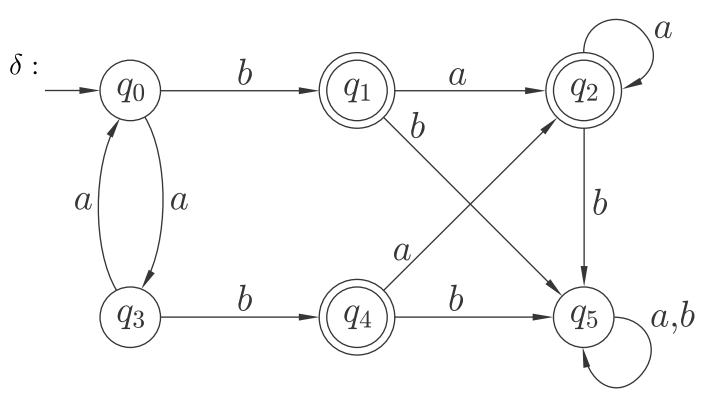
\includegraphics[width=0.8\textwidth]{pics/Blatt9.png}
	\end{center}
\end{figure}

\textbf{Wiederholung:} Approximation $\sim_k$ von $\sim_\A$:
\begin{itemize}
	\item $q\sim_0 q':\Longleftrightarrow (q\in F\Leftrightarrow q'\in F)$
	\item $q\sim_{k+1} q':\Longleftrightarrow(q\sim_k q\wedge\forall a\in\Sigma:\delta(q,a)\sim_k\delta(q',a)$
\end{itemize}
In Aufgabe 8.4 (b) wurde gezeigt:
\begin{align*}
	(\exists k\in\N:\sim_k=\sim_{k+1})\implies\sim_k=\sim_\A
\end{align*}
Bestimme also $\sim_\A$ schrittweise durch Approximation:
\begin{itemize}
	\item $Q|_{\sim_0}=\big\lbrace\lbrace q_1,q_2,q_4\rbrace,\lbrace q_0,q_3,q_5\rbrace\big\rbrace$ Wir trennen also die Endzustände von den Nichtendzuständen (dies ist immer der erste Schritt). Nun ``verfeinern'' wir diese Zerlegung.
	\item $Q|_{\sim_1}=\big\lbrace\lbrace q_1,q_2,q_4\rbrace,\lbrace q_0,q_3,\rbrace,\lbrace q_5\rbrace\big\rbrace$ (``Bleibt $q_i$ in der Äquivalenzklasse?'')
	\item $Q|_{\sim_2}=\big\lbrace\lbrace q_1,q_2,q_4\rbrace,\lbrace q_0,q_3\rbrace,\lbrace q_5\rbrace\big\rbrace=Q|_{\sim_1}\implies \sim_2=\sim_1=\sim_\A$ 
\end{itemize}

Mit $\tilde{q}:=[q|_{\sim_\A}=\lbrace q'\in Q\mid  q\sim_\A g'\rbrace$ erhalten wir:
\begin{align*}
	\tilde{A}&=\big(\lbrace\tilde{q}_1,\tilde{q}_0,\tilde{q}_5\rbrace,\lbrace a,b\rbrace,\tilde{q}_0,\tilde{\delta},
	\underbrace{\lbrace\tilde{q}_1,\tilde{q}_2,\tilde{q}_4\rbrace}_{=\lbrace\tilde{q}_1\rbrace}\big)\mit\\
	\tilde{\delta}(\tilde{q},x)&:=\widetilde{\delta(q,x)}\mit x\in\lbrace a,b\rbrace
\end{align*}

Quotientenautomat $\tilde{\A}$:
\usetikzlibrary{positioning,automata}
\begin{tikzpicture}[shorten >=1pt,node distance=2.7cm,on grid]
  \node[state,initial]   (q_0)                {$\tilde{q}_0$};
  \node[state, accepting](q_1) [right=of q_0] {$\tilde{q}_1$};
  \node[state] (q_5) [right=of q_1] {$\tilde{q}_5$};
  \path[->] (q_0) edge [loop above] node [above] {a} ()
                  edge [bend left=0] node [above] {b} (q_1)
            (q_1) edge [loop above] node [above] {a} ()
            	  edge [bend left=0] node [above] {b} (q_5)
            (q_5) edge [loop above] node [above] {a,b} ();
\end{tikzpicture}

\subsection{Aufgabe 2}
Gegeben sei der DEA
\begin{align*}
	\A=\Big(\lbrace q_0,\ldots,q_8\rbrace,\lbrace a,b\rbrace, q_0,\delta,\lbrace q_3,q_6\rbrace\Big)
\end{align*}
mit
\begin{figure}[H] 
	\begin{center}
		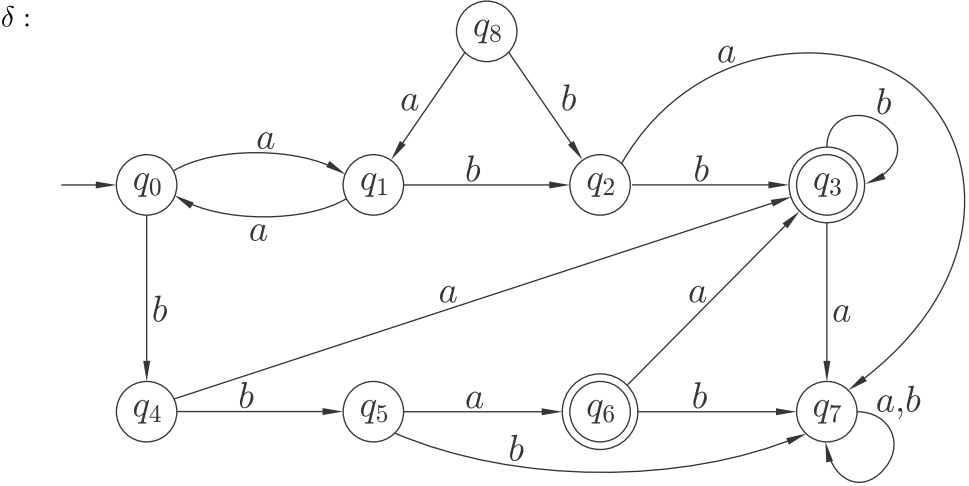
\includegraphics[width=0.8\textwidth]{pics/Blatt9_2.png}
	\end{center}
\end{figure}

Der Vorlesung folgend bezeichne $\A_0$ den zu $\A$ äquivalenten Automaten, den man erhält, indem man alle in $\A$ unerreichbaren Zustände entfernt (und $\delta$ entsprechend anpasst oder einschränkt). 
Hier entspricht $\A_0$ also $\A$ ohne $q_8$.\nl
Nun berechnen wir den Quotientenautomaten $\tilde{\A}_0$ von $\A_0$.\\
Bestimme zuerst $\tilde{\A}_0$: ($Q=\lbrace q_0,\ldots,q_7\rbrace$!)
\begin{itemize}
	\item $Q|_{\sim_0}=\big\lbrace q_3,q_6\rbrace,\lbrace q_0,q_1,q_2,q_4,q_5,q_7\rbrace\big\rbrace$
	\item $Q|_{\sim_1}=\big\lbrace q_3\rbrace,\lbrace q_6\rbrace,\lbrace q_0,q_1,q_7\rbrace,\lbrace q_2\rbrace,\lbrace q_4,q_5\rbrace\big\rbrace$
	% q_5 -> q_3 (in erster Klasse)
	% q_0,q_1 bleiben äquivalent
	\item $Q|_{\sim_2}=\big\lbrace q_3\rbrace,\lbrace q_6\rbrace,\lbrace q_0\rbrace,\lbrace q_1\rbrace,\lbrace q_7\rbrace,\lbrace q_2\rbrace,\lbrace q_4\rbrace,\lbrace q_5\rbrace\big\rbrace$
	\item $Q|_{\sim_3}=Q|_{\sim_2}\implies\sim_3=\sim_2=\sim_{\A_0}$
\end{itemize}
Hier sind also alle Zustände paarweise nicht äquivalent zueinander. 
Der zu $\A$ reduzierte DEA $\A_{\text{red}}$ ist also:
\begin{align*}
	\A_{\text{red}}=\tilde{\A}_0\cong\A_0
\end{align*}
Das heißt, also $\tilde{\A}_0$ isomorph zu $\A_0$ ist (also gleich bis auf Umbenennung der Zustände). Also im Prinzip ist gar nichts passiert (außer, dass $q_8$ entfernt wurde).

\subsection{Aufgabe 3}
Diese Aufgabe zeigt, warum es trotzdem sinnvoll sein kann, Nicht-DEAs zu verwenden.

\subsubsection{Aufgabe 3 a)}
\begin{align*}
	L(\A_n)
	&=\big\lbrace q\in\lbrace a,b\rbrace^\ast\mid\text{der $n$-te Buchstabe von hinten in $w$ ist ein }a\big\rbrace\\
	&=\lbrace a,b\rbrace^\ast\cdot\lbrace a\rbrace\cdot\lbrace a,b\rbrace^{n-1}
\end{align*}

\subsubsection{Aufgabe 3 b)}
$\A_3$:\\
\usetikzlibrary{positioning,automata}
\begin{tikzpicture}[shorten >=1pt,node distance=2.7cm,on grid]
  \node[state,initial]   (q_0)                {$q_0$};
  \node[state](q_1) [right=of q_0] {$q_1$};
  \node[state] (q_2) [right=of q_1] {$q_2$};
  \node[state, accepting] (q_3) [right=of q_2] {$q_3$};
  \path[->] (q_0) edge [loop above] node [above] {a,b} ()
                  edge [bend left=0] node [above] {a} (q_1)
            (q_1) edge [bend left=0] node [above] {a,b} (q_2)
            (q_2) edge [bend left=0] node [above] {a,b} (q_3);
\end{tikzpicture}

Berechnung eines äquivalenten DEA $\A_3'$ durch Potenzmengenkonstruktion:
%TODO tikz-Bild

Umbenennung der Zustände des Quotientenautomaten:
\begin{itemize}
	\item $p_0:=\lbrace q_0\rbrace$
	\item $p_1:=\lbrace q_0,q_1\rbrace$
	\item $p_2:=\lbrace q_0,q_1,q_2\rbrace$
	\item $p_3:=\lbrace q_0,q_2\rbrace$
	\item $p_4:=\lbrace q_0,q_1,q_2,q_3\rbrace$
	\item $p_5:=\lbrace q_0,q_2,q_3\rbrace$
	\item $p_6:=\lbrace q_0,q_1,q_3\rbrace$
	\item $p_7:=\lbrace q_0,q_3\rbrace$
\end{itemize}

Berechnung des Quotientenautomaten (nach Konstruktion gibt es keine unerreichbaren Zustände in obiger Potenzmengenkonstruktion):
\begin{itemize}
	\item $Q|_{\sim_0}=\big\lbrace\lbrace p_4,p_5,p_6,p_7\rbrace,\lbrace p_0,p_1,p_2,p_3\rbrace\big\rbrace$
	\item $Q|_{\sim_1}=\big\lbrace\lbrace p_4,p_5\rbrace,\lbrace p_6,p_7,\lbrace p_0,p_1\rbrace,\lbrace p_2,p_3\rbrace\big\rbrace$
	\item $Q|_{\sim_2}=\big\lbrace\lbrace p_4\rbrace,\lbrace p_5\rbrace,\lbrace p_6\rbrace,\lbrace p_7,\lbrace p_0\rbrace,\lbrace p_1\rbrace,\lbrace p_2\rbrace,\lbrace p_3\rbrace\big\rbrace=Q|_{\sim_3}\implies\sim_2=\sim_3=\sim_{\A'}$
\end{itemize}
Daher gilt: $\A_3\cong(\A_3')_{\text{red}}$ (analog zu Aufgabe 2).

\subsubsection{Aufgabe 3 c)}
Seien also $x=x_1 x_2\hdots x_n\in\lbrace a,b\rbrace^n$ und $y=y_1 y_2\hdots y_n\in\lbrace a,b\rbrace^n$ mit $x\neq y$.\\
Zu zeigen: $x\not\cong_{L(\A_n} y$, d.h.
\begin{align*}
	\exists w\in\lbrace a,b\rbrace^\ast:\big(xw\in L(\A_n)\wedge yw\not\in L(\A_n)\big)\vee\big(xw\not\in L(\A_n)\wedge yw\in L(\A_n)\big)
\end{align*}
Da $x\neq y$, gibt es einen kleinsten Index $j\in\lbrace1,\ldots,n\rbrace$ so, dass $x_j\neq y_j$ (die erste Position von links, an der sich $x$ und $y$ unterscheiden). 
Setze dann 
\begin{align*}
	w:=a^{j-1}
\end{align*}
Dann gibt es zwei Möglichkeiten für $x_j,y_j$:
\begin{enumerate}
	\item $x_j=a$ und $y_j=b$:
	\begin{align*}
		xw&=x_1\hdots x_{j-1}\underbrace{ a x_{j+1}\hdots x_n\underbrace{a\hdots a}_{j-1\text{ viele}}}_{n-(j-1)+(j-1)=n}\in L(\A_n)\\
		yw&=y_1\hdots y_{j-1}\underbrace{ b y_{j+1}\hdots x_n\underbrace{a\hdots a}_{j-1\text{ viele}}}_{n-(j-1)+(j-1)=n}\not\in L(\A_n)
	\end{align*}
	\item $x_j=b$ und $y_j=a$: analog.
\end{enumerate}

Alle paarweise verschiedenen Worte der Länge $n$ über dem Alphabet über $\lbrace a,b\rbrace$ sind nicht äquivalent bzgl. $\cong_{L(\A_n)}$. Da es $2^n$ verschiedene Wörter über $\lbrace a,b\rbrace$ gibt, so gibt es auch mindestens $2^n$ verschiedene Äquivalenzklassen von $\cong_{L(\A_n)}$. Aus Lemma 2.15 (4) folgt damit, dass ein minimaler Automat mindestens $2^n$ Zustände hat.

% This work is licensed under the Creative Commons
% Attribution-NonCommercial-ShareAlike 4.0 International License. To view a copy
% of this license, visit http://creativecommons.org/licenses/by-nc-sa/4.0/ or
% send a letter to Creative Commons, PO Box 1866, Mountain View, CA 94042, USA.

\section{Aufgabenblatt 10}
\subsection*{Aufgabe $\ast$)}
Gegeben ist der $\varepsilon$-NEA
\begin{align*}
	\A=\Big(\lbrace q_0,\ldots,q_4\rbrace,\lbrace a,b\rbrace,q_0,\Delta,\lbrace q_2\rbrace\Big)
\end{align*}

\usetikzlibrary{positioning,automata}
\begin{tikzpicture}[shorten >=1pt,node distance=2.7cm,on grid]
  \node[state,initial]   	(q_0)                		{$q_0$};
  \node[state] 				(q_1) [above right=of q_0] 	{$q_1$};
  \node[state, accepting] 	(q_2) [right=of q_1] 		{$q_2$};
  \node[state] 				(q_3) [below right=of q_0] 	{$q_3$};
  \node[state] 				(q_4) [right=of q_3]		{$q_4$};
  \path[->] (q_0) edge [bend left=0] node [above] {a} (q_1)
                  edge [bend left=0] node [above] {b} (q_3)
            (q_1) edge [bend left=0] node [above] {$\varepsilon$} (q_2)
            	  edge [bend left=0] node [left] {a,b} (q_3)
            (q_2) edge [bend left=0] node [right] {a} (q_3)
                  edge [bend left=0] node [right] {a} (q_4)
            (q_3) edge [bend left=0] node [above] {b} (q_4)
            (q_4) edge [loop right] node [right] {a} ();
\end{tikzpicture}

(Es fällt auf, dass $L(\A)=\lbrace a\rbrace$ ist.)
Zuerst entfernen wir die $\varepsilon$-Transitionen auf naheliegende Weise:

\usetikzlibrary{positioning,automata}
\begin{tikzpicture}[shorten >=1pt,node distance=2.7cm,on grid]
  \node[state,initial]   	(q_0)                		{$q_0$};
  \node[state, accepting]   (q_1) [above right=of q_0] 	{$q_1$};
  \node[state, accepting] 	(q_2) [right=of q_1] 		{$q_2$};
  \node[state] 				(q_3) [below right=of q_0] 	{$q_3$};
  \node[state] 				(q_4) [right=of q_3]		{$q_4$};
  \path[->] (q_0) edge [bend left=0] node [above] {a} (q_1)
                  edge [bend left=0] node [above] {b} (q_3)
            (q_1) edge [bend left=0] node [above] {a} (q_4) %Diese Transition wurde geändert
            	  edge [bend left=0] node [left] {a,b} (q_3)
            (q_2) edge [bend left=0] node [right] {a} (q_3)
                  edge [bend left=0] node [right] {a} (q_4)
            (q_3) edge [bend left=0] node [above] {b} (q_4)
            (q_4) edge [loop right] node [right] {a} ();
\end{tikzpicture}

Wichtig ist hierbei, dass nun $q_1$ auch ein Endzustand geworden ist.
Nun erzeugen wir den äquivalenten DEA mithilfe der Potenzmengenkonstruktion:

\usetikzlibrary{positioning,automata}
\begin{tikzpicture}[shorten >=1pt,node distance=2.7cm,on grid]
  \node[state,initial]   	(q_0)                		{$\lbrace q_0\rbrace$};
  \node[state, accepting]   (q_1) [above right=of q_0] 	{$\lbrace q_1\rbrace$};
  \node[state]			 	(q_3q_4) [right=of q_1] 		{$\lbrace q_3,q_4\rbrace$};
  \node[state] 				(q_3) [below right=of q_0] 	{$\lbrace q_3\rbrace$};
  \node[state]			 	(q_4) [right=of q_3]		{$\lbrace q_4\rbrace$};
  \node[state]				(T)	  [below right =of q_3q_4] {$\emptyset$};
  \path[->] (q_0) edge [bend left=0] node [above] {a} (q_1)
                  edge [bend left=0] node [above] {b} (q_3)
            (q_1) edge [bend left=0] node [above] {a} (q_3q_4)
            	  edge [bend left=0] node [left] {b} (q_3)
            (q_3q_4) edge [bend left=0] node [right] {a,b} (T)
                  %edge [bend left=0] node [right] {a} (q_4)
            (q_3) edge [bend left=0] node [above] {b} (q_4)
            	  edge [bend left=30] node [below] {a} (T)
            (q_4) edge [loop right] node [right] {a} ()
            	  edge [bend left=0] node [below] {b} (T)
           	(T)   edge [loop right] node [above] {a,b} ();
\end{tikzpicture}

Den unerreichbaren Zustand $q_2$ braucht man nicht beachten. Den Papierkorbzustand $\emptyset$ nicht vergessen. Also ist der äquivalente DEA:
\begin{align*}
	\A'&=\Big(\big\lbrace q_0\rbrace,\lbrace q_1\rbrace,\lbrace q_3\rbrace,\lbrace q_3,q_4\rbrace,\lbrace q_4\rbrace,\emptyset\big\rbrace,\lbrace a,b\rbrace,\lbrace q_0\rbrace,\delta,\big\lbrace\lbrace q_1\rbrace\big\rbrace\Big)\\
	\overset{\text{Umbennung}}&{=:}
	\Big(\underbrace{\lbrace p_0, p_1,p_3,p_2,p_4, p_5\rbrace}_{=:P},\lbrace a,b\rbrace,p_0,\delta,\lbrace p_1\rbrace\Big)
\end{align*}

Da $\A'$ keine unerreichbaren Zustände mehr besitzt, gilt $\A_0=\A'$.
Um $\A_{\text{red}}$ zu berechnen, berechnen wir $\sim_{\A}$ schrittweise durch $\sim_k$:
\begin{itemize}
	\item $P|_{\sim_0}=\big\lbrace\lbrace p_1\rbrace,\lbrace p_0,p_2,p_3,p_4,p_5\rbrace\big\rbrace$ (Startzustände und Endzustände trennen)
	\item $P|_{\sim_1}=\big\lbrace\lbrace p_1\rbrace,\lbrace p_0\rbrace,\lbrace p_2,p_3,p_4,p_5\rbrace\big\rbrace$
	\item $P|_{\sim_2}=\big\lbrace\lbrace p_1\rbrace,\lbrace p_0\rbrace,\lbrace p_2,p_3,p_4,p_5\rbrace\big\rbrace$
\end{itemize}
Es gilt also $\sim_2=\sim_1\implies\sim_\A=\sim_1$. 
Der Quotientenautomat
\begin{align*}
	\tilde{A}&=\big(\tilde{Q},\Sigma,\tilde{q}_0,\tilde{\delta},\tilde{F}\big)\mit\\
	\tilde{Q}&=\big\lbrace\lbrace p_1\rbrace,\lbrace p_0\rbrace,\lbrace p_2,p_3,p_4,p_5\rbrace\big\rbrace
	=
	\big\lbrace [p_1]_{\sim},[p_0]_\sim,[p_2]_\sim\big\rbrace\\
	\Sigma&=\lbrace a,b\rbrace\\
	\tilde{q}_0&=\lbrace p_0\rbrace=[p_0]_\sim\\
	\tilde{\delta}&=\left\lbrace
		\begin{array}{l}
			\big([p_0]_{\sim},a,[p_1]_{\sim}\big), \big([p_0]_{\sim},b,[p_2]_{\sim}\big),\\
			\big([p_1]_{\sim},a,[p_2]_{\sim}\big), \big([p_1]_{\sim},b,[p_2]_{\sim}\big),\\
			\big([p_2]_{\sim},a,[p_2]_{\sim}\big), \big([p_2]_{\sim},b,[p_2]_{\sim}\big)
		\end{array}
	\right\rbrace\\
	\tilde{F}&=\big\lbrace \lbrace p_1\rbrace\big\rbrace=\big\lbrace [p_1]_\sim\big\rbrace
\end{align*}
erfüllt also
\begin{align*}
	\A_{\text{red}}=\tilde{\A_0}\cong\A_0=\A'
\end{align*}
und insbesondere gilt
\begin{align*}
	L\big(\A_\red\big)=\lbrace a\rbrace.
\end{align*}

\begin{tikzpicture}[shorten >=1pt,node distance=2.7cm,on grid]
  \node[state,initial]   	(q_0)                		{$[p_0]_{\sim}$};
  \node[state, accepting]   (q_1) [above right=of q_0] 	{$[p_1]_{\sim}$};
  \node[state] 				(q_2) [below right=of q_0] 	{$[p_2]_{\sim}$};
  \path[->] (q_0) edge [bend left=0] node [above] {a} (q_1)
                  edge [bend left=0] node [above] {b} (q_2)
            (q_1) edge [bend left=0] node [right] {a,b} (q_2)
            (q_2) edge [loop right]  node [above] {a,b} ();
\end{tikzpicture}

\subsection{Aufgabe 1}
\textbf{Konvention.} Bei mir ist $\N:=\lbrace 1,2,3,\ldots\rbrace$.\nl
Meine Idee (geht sicher viel eleganter):\\
Da es sehr viele Zerlegungsmöglichkeiten pro Wort $w$ gibt, ist es geschickter zu schauen, für welche $y\in\Sigma^+$ überhaupt die Eigenschaft 
\begin{align*}
	\exists x,z\in\Sigma^\ast:\forall k\in\N:xy^kz\in L(\A)
\end{align*}
gilt.
Man sieht, dass nur $y\in\lbrace c,cd,dc\rbrace=:M$ dies erfüllen. Nun gehen wir $w$ einzeln durch und schauen uns nur die Zerlegungen an, bei der $y\in M$ gilt (denn nur die sind interessant). Da $x,z=\varepsilon$ möglich, erhalten wir genau diese möglichen Zerlegungen durch \textit{Stringvergleich}, d.h. wir schauen, ob ein $p\in M$ existiert, welches ein Substring von dem festen $w$ ist. Also: (Nutze Kurzschreibweise $\alpha|\beta|\gamma$ für Zerlegung des Wortes $w$ in $x=\alpha$, $y=\beta$ und $z=\gamma$)
\begin{itemize}
	\item $w=adc$: Mögliche Zerlegungen: 
	\begin{itemize}
		\item $ad|c|\varepsilon$: ist in $L(\A)$, aber $c$ dann nicht mehr loopbar.
		\item $a|dc|\varepsilon$: ist in $L(\A)$ und erfüllt \eqref{eqAufgabe1}.
	\end{itemize}
	\item $w=cda$ ist gar nicht in $L(\A)$, weshalb keine solche Zerlegungen existieren können, die \eqref{eqAufgabe1} erfüllen. 
	\item $w=bcdc$ Mögliche Zerlegungen: 
	\begin{itemize}
		\item $b|c|dc$: erfüllt \eqref{eqAufgabe1}.
		\item $bcd|c|\varepsilon$: erfüllt \eqref{eqAufgabe1} nicht, da $c$ nicht mehr "geloopt" werden kann, nach $acd$ gelesen wurde.
		\item $b|cd|c$: erfüllt \eqref{eqAufgabe1}.
		\item $bc|dc|\varepsilon$: erfüllt \eqref{eqAufgabe1}.
	\end{itemize}
	\item $w=acdc$ Mögliche Zerlegungen: 
	\begin{itemize}
		\item $a|c|dc$: erfüllt \eqref{eqAufgabe1}.
		\item $acd|c|\varepsilon$ erfüllt \eqref{eqAufgabe1} nicht, da $c$ dann nicht mehr geloopt werden kann.
		\item $ac|dc|\varepsilon$ erfüllt \eqref{eqAufgabe1}.
		\item $a|cd|c$ erfüllt \eqref{eqAufgabe1}.
	\end{itemize}
\end{itemize}
Somit erhalten wir für $adc$ 1, für $cda$ 0, für $bcdc$ 3 und für $acdc$ 3 Zerlegungen, die die gesuchten Eigenschaft erfüllen:

\begin{align}\label{eqAufgabe1}
	\forall k\in\N:xy^kz\in L(\A)
\end{align}

\textbf{Tutor-Lösung: (stimmt mit meiner überein)}
\begin{itemize}
	\item $w=adc\in L(\A)$: kein Zerlegung möglich bei der $y$ auch wegfallen kann
	\item $w=cda\not\in L(\A)$: keine "pumpbare" Zerlegung möglich, da nicht in der Sprache
	\item $w=bcdc\in L(\A)$:
	\begin{itemize}
		\item $x=b,\qquad,y=c,\qquad z=dc$
		\item $x=b,\qquad y=cd,\qquad z=c$
		\item $x=bc,\qquad y=dc,\qquad z=\varepsilon$
	\end{itemize}
	\item $w=acdc\in L(\A)$:
	\begin{itemize}
		\item $x=a,\qquad y=c,\qquad z=dc$
		\item $x=ac,\qquad y=dc,\qquad z=\varepsilon$
		\item $x=a,\qquad y=cd,\qquad z=\varepsilon$ 
	\end{itemize}
\end{itemize}

Beachte: falls man $0\in\N$ annimmt, entfallen noch einige Fälle oben.

\subsection{Aufgabe 2}
Die Sprache
\begin{align*}
	L:=\big\lbrace a^p\mid p\text{ ist Primzahl}\big\rbrace\mit\Sigma:=\lbrace a\rbrace
\end{align*}
ist nicht erkennbar.

\begin{proof}
	Wir führen einen Widerspruchsbeweis: Angenommen, $L$ ist erkennbar.
	Dann folgt aus dem Pumping-Lemma (3.1): Es gibt $n_0\in\N_{\geq1}$ so, dass jedes Wort $w\in L$ mit $|w|\geq n_0$ sich zerlegen lässt in $w=xyz$ mit $y\neq\varepsilon$ und $xy^kz\in L$ für alle $k\geq0$.
	Sei also $w=a\ldots a\in L$ beliebig mit $p\geq n_0$. Also gilt
	\begin{align*}
		&w=\underbrace{a\ldots a}_{p\geq n_0\text{ Stück}}\overset{!}= xy^k z\\
		&\implies \exists l,m,n\in\N_{\geq0}: w=a^p=a^l a^m a^n\\
		&\implies p=l+m+n
	\end{align*}
	Nach Voraussetzung ist $p$ eine Primzahl und nach Pumpinglemma gilt:
	\begin{align*}
		&x y^k z\in L &\forall k\in\N_{\geq0}\\
		&\implies l+m\cdot k+ n\text{ ist Primzahl} &\forall k\in\N_{\geq0}
	\end{align*}
	Dies ist aber im Allgemeinen keine Primzahl (was ich gerade leider nicht für alle Fälle zeigen kann...).\\
	Widerspruch! Somit ist $L$ nicht erkennbar.
\end{proof}

\begin{proof}[Beweis des Tutors.]\enter
	\textbf{Pumping-Lemma (vereinfacht)}:\\
	Für jede erkennbare Sprache $L$ existiert ein $n_0\in\N$ so, dass\\
	für alle Wörter $w\in L$ mit $|w|\geq n_0$\\
	existiert eine Zerlegung $w=xyz$ mit $y\neq\varepsilon$ so, dass\\
	für alle $k\in\N$ gilt: $xy^kz\in L$.\nl
	Beweis durch Widerspruch:
	Angenommen, $L$ wäre erkennbar. Dann gilt das Pumpinglemma (vereinfacht) auch für $L$.
	Sei $p$ ein Primzahl mit $p\geq n_0$ (existiert nach Satz von Euklid: Es gibt unendlich viele Primzahlen).
	Dann gilt:
	$a^p\in L$ und $|a^p|\geq n_0$.
	Damit muss es eine Zerlegung von $a^p=xyz$ geben $\rightsquigarrow x=a^n,y=a^m,z=a^{n_2}$ mit $n_1,n_2,m\in\N$ und $m>0$.
	Also gilt $p=n_1+n_2+m$. 
	Definiere $n:=n_1+n_2$.
	Da $a^p=a^{m+n}\in L$, folgt aus dem Pumping-Lemma,
	dass auch $a^{n+k\cdot m}\in L$ für alle $k\in\N$.
	Insbesondere für $k=n$ %Die Idee, die mir fehlte!
	gilt $a^{n+n\cdot m}\in L$.
	Aber falls $n\neq1$ (also $n>1$ oder $n=0$) ist $n+n\cdot m=n\cdot(m+1)$ keine Primzahl!\\
	Falls $n=1$, dann müsste $a^{n+0\cdot m}=a^n=a\in L$ gelten. Widerspruch!
\end{proof}

\subsection{Aufgabe 3}
Die Sprache
\begin{align*}
	L:=\Big\lbrace w\mid w=1^k\text{ für }k\geq0\text{ oder }w=0^j1^p\text{ für }j\geq1\text{ und }p\text{ Primzahl}\Big\rbrace\\
	\mit\Sigma=\lbrace0,1\rbrace
\end{align*}
ist nicht erkennbar.

\begin{proof}
	\textbf{Pumping-Lemma (verschärft, Änderungen unterstrichen)}:\\
	Für jede erkennbare Sprache $L$ existiert ein $n_0\in\N$ so, dass\\
	%für alle Wörter $w\in L$ mit $|w|\geq n_0$ 
	\underline{für alle Wörter $u,v,w$ mit $uvw\in L$ und $|w|\geq n_0$}\\
	existiert eine Zerlegung $\underline{v}=xyz$ mit $y\neq\varepsilon$ so, dass\\
	für alle $k\in\N$ gilt: $xy^kz\in L$.\nl
	Das vereinfachte Pumpinglemma kann hier zwar auch wieder angewendet werden, hilft uns aber nicht, da
	alle $w\in L$ mit $|w|>0$ "pumpbar" zerlegt werden können:
	\begin{itemize}
		\item $w=1^k\rightsquigarrow x=1^{k-1},y=1,z\varepsilon$
		\item $w=0^j 1^p\rightsquigarrow x=\varepsilon,y=0^j,z=1^p$
	\end{itemize}
	Es gibt also eine gültige Zerlegung, weshalb wir mit dem vereinfachten Pumpinglemma keinen Widerspruch herleiten können.
	Mit dem Pumping-Lemma in verschärfter Form kann das Ergebnis aus Aufgabe 10.2 genutzt werden:
	Sei $p$ eine Primzahl mit $p\geq n_0$. Zerlege dann das Wort $01^p$ in $u=0$, $v=1^p$ und $w=\varepsilon$.
	Es gilt $01^p\in L$ und $|v|\geq n_0$.
	Zerlege dann $v$ nun wie in 10.2 gezeigt.
\end{proof}

\subsection{Aufgabe 4}
\textbf{Satz 4.1} Ist $L$ erkennbar, so ist auch $L^\ast$ erkennbar.

\begin{proof}
	%Erinnerung: Eine Sprache $L$ ist per Definition erkennbar, wenn es einen NEA $\A$ gibt, der $L$ akzeptiert, d.a. $L=L(\A)$.\nl
	Da $L$ erkennbar ist, gibt es per Definition einen NEA
	\begin{align*}
		\A:=(Q,\Sigma,q_0,\Delta,F)
	\end{align*}
	mit $L(\A)=L$. 
	Sei nun $q_{0\varepsilon}\not\in Q$ und setze
	\begin{align*}
		\A_\varepsilon&:=\Big(Q\cup\lbrace q_{0\varepsilon}\rbrace,\Sigma,q_{0\varepsilon},\Delta_\varepsilon,\lbrace q_{0\varepsilon}\rbrace\Big)\\
		\Delta_\varepsilon&:=\Delta\cup\underbrace{\big\lbrace(f,\varepsilon,q_{0\varepsilon}):f\in F\big\rbrace}_{
			=\big(F\times\lbrace\varepsilon\rbrace\times\lbrace q_{0\varepsilon}\rbrace\big)
		}\cup\big\lbrace(q_{0\varepsilon},\varepsilon,q_{0})\big\rbrace\Big)
	\end{align*}
	
	
  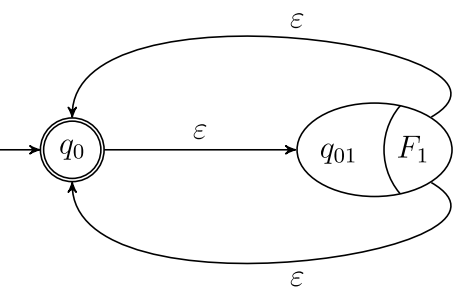
\includegraphics[width=0.7\textwidth]{pics/Blatt10_4.png}
  
  Offenbar ist $\A_\varepsilon$ ein $\varepsilon$-NEA. Mit Lemma 1.12 bekommt man einen zu $\A_\varepsilon$ äquivalenten NEA, nennen wir ihn $\A_{\text{NEA}}$. Äquivalent bedeutet $L(\A_\varepsilon)=L(\A_{\text{NEA}})$.\nl
  Bleibt noch zu zeigen, dass $L(\A_\varepsilon)=L^\ast$ gilt. 
  Sei also $w\in L^\ast$.
  Dann gibt es ein $n\in\N$ so, dass $w\in\bigcup\limits_{i=0}^n L$ ist. Man sieht leicht, dass $w\in L(\A_\varepsilon)$ liegen muss. (Das formal aufzuschreiben ist ein wenig sperrig.)
\end{proof}

\subsection{Aufgabe 5}
Folgende Automatenklassen sind in ihrer Ausdrucksstärke gleichmächtig zueinander:
NEA, $\varepsilon$-NEA (entfernen von $\varepsilon$-Transitionen), NEA mit Wortübergängen (Zwischenzustände einführen), DEA (Potenzmengenkonstruktion)\\
Transitionssysteme sind \underline{nicht} äquivalent zu obigen.\nl
Beweise oder Widerlege:
\begin{enumerate}[label=\alph*)]
	\item $L$ erkennbar $\implies\exists\varepsilon$-NEA $\A:L(\A)=L$.\\
	Stimmt, denn:
	\begin{align*}
		L\text{ erkennbar}
		\overset{\text{Def 1.6}}&\Longleftrightarrow
		\exists\text{NEA}\A_N:L(\A_N)=L\\
		\overset{\text{Lemma 10}}&\Longleftrightarrow
		\exists\varepsilon\text{-NEA }\A:L(\A)\overset{\text{Def 1.6}}{=}L(\A_N)=L
	\end{align*}
	\item $\exists$ NEA mit Wortübergängen mit $L(\A)=L\implies L$ erkennbar.\\
	Stimmt, denn:
	\begin{align*}
		&\exists\text{ NEA $\A$ mit Wortübergängen mit }L(\A)=L\\
		\overset{\text{Satz 1.9}}&\implies
		\exists\text{ NEA }\A_N:L(\A_N)\overset{\text{Def 1.6}}=L(\A)=L\\
		\overset{\text{Def 1.6}}&\implies
		L\text{ erkennbar}
	\end{align*}
	\item $\exists$ Transitionssystem $\A$ mit $L(\A)=L\implies L$ erkennbar\\
	Das stimmt nicht, Gegenbeispiel:
	\begin{align*}
		L:=\Big\lbrace a^p:p\text{ ist Primzahl }\Big\rbrace
	\end{align*}
	Transitionssystem: (wird endliche Kette, Endzustände sind Primzahlen)
	\item $L$ erkennbar und $L\subseteq L'\implies L'$ erkennbar\\
	Stimmt nicht, Gegenbeispiel:
	\begin{align*}
		L:=\lbrace aa\rbrace\qquad
		L':=\Big\lbrace a^p:p\text{ ist Primzahl }\Big\rbrace
	\end{align*}
	\item $L$ erkennbar und $L'\subseteq L\implies L'$ erkennbar.\\
	Stimmt nicht, Gegenbeispiele:
	\begin{align*}
		&L=\Big\lbrace a^n:n\in\N\big\rbrace,& l'=\big\lbrace a^p:p\text{ ist Primzahl }\Big\rbrace\\
		&L_2=\Sigma^\ast, &\Big\lbrace a^n b^n:n\in\N\Big\rbrace
	\end{align*}
	\item $L_1,L_2$ erkennbar $\implies L:=L_1\cap L_2$ erkennbar.\\
	Stimmt, wegen Satz 4.1.
	\item Wenn es ein $n\in\N$ gibt, so dass $\cong_L$ (Nerode-Rechtskongruenz) höchstens $n$ Äquivalenzklassen hat, so ist $L$ erkennbar.\\
	Ja, dies ist eine Richtung des Satzes von Myhill-Nerode
	($L$ ist erkennbar / regulär $\Longleftrightarrow \, \cong_L$ hat endlichen Index / endliche viele Äquivalenzklassen)
\end{enumerate}


% This work is licensed under the Creative Commons
% Attribution-NonCommercial-ShareAlike 4.0 International License. To view a copy
% of this license, visit http://creativecommons.org/licenses/by-nc-sa/4.0/ or
% send a letter to Creative Commons, PO Box 1866, Mountain View, CA 94042, USA.

\section{Aufgabenblatt 11}
\subsection*{Aufgabe $\ast$)}
%TODO

\subsection*{Aufgabe $\ast\ast$)}
%TODO

\subsection{Aufgabe 1}
Seien $r,s$ reguläre Ausdrücke, Beachte $r=s:\Longleftrightarrow L(r)=L(s)$ (eigentlich $r\equiv s$). Dann gilt:
\begin{enumerate}[label=\alph*)]
	\item $r+s=s+r$
	\item $(r+s)+t=r+(s+t)$
	\item $(rs)t=r(st)$
	\item $r(s+t)=rs+rt$
	\item $\emptyset^\ast=\varepsilon$
	\item $(r^\ast)^\ast=r^\ast$
	\item $r^\ast=rr^\ast+\varepsilon$
	\item $(\varepsilon+r)^\ast=r^\ast$
\end{enumerate}

\begin{proof}
	\underline{Zeige a):}
	\begin{align*}
		r+s
		\overset{\text{Not}}&=		
		L(r+s)
		\overset{\text{Def}}=
		L(r)\cup L(s)
		\overset{\text{Kommu. von }\cup}=
		L(s)\cup L(r)
		\overset{\text{Def}}=
		L(s+r)
		\overset{\text{Not}}=	
		s+r
	\end{align*}
	\underline{Zeige b):}
	\begin{align*}
		L\big((r+s)+t\big)
		\overset{\text{}}&=
		L(r+s)\cup L(t)\\
		\overset{\text{}}&=
		\big(L(r)\cup L(s)\big)\cup L(t)\\
		\overset{\text{Asso. von }\cup}&=
		L(r)\cup\big(L(s)\cup L(t)\big)\\
		\overset{\text{}}&=
		L(r)\cup L(s+t)\\
		\overset{\text{}}&=
		L\big(r+(s+t)\big)
	\end{align*}
	
	\underline{Zeige c):} "Ersetze Punkt durch Konkatenationsoperator auf Sprachen":
	\begin{align*}
		L\big((r\cdot s)\cdot t\big)
		\overset{\text{}}&=
		L(r\cdot s)\cdot L(t)\\
		\overset{\text{}}&=
		\big(L(r)\cdot L(s)\big)\cdot L(t)\\
		\overset{\text{}}&=
		\big\lbrace ab:a\in L(r)\cdot L(s)\wedge b\in L(t)\big\rbrace\\
		\overset{\text{}}&=
		\Big\lbrace ab:a\in\big\lbrace cd:c\in L(r)\wedge d\in L(s)\big\rbrace\wedge b\in L(t)\Big\rbrace\\
		\overset{\text{}}&=
		\Big\lbrace cdb:\big(c\in L(r)\wedge d\in L(s)\big)\wedge b\in L(t)\Big\rbrace\\
		\overset{\text{Asso. von }\wedge}&=
		\Big\lbrace cdb:c\in L(r)\wedge\big(d\in L(s)\wedge b\in L(t)\big)\Big\rbrace\\
		\overset{\text{}}&=
		\Big\lbrace ce:c\in L(r)\wedge e\in\big\lbrace db:d\in L(s)\wedge b\in L(t)\big\rbrace\Big\rbrace\\
		\overset{\text{}}&=
		\big\lbrace ce:c\in L(r)\wedge e\in L(s)\cdot L(t)\big\rbrace\\
		\overset{\text{}}&=
		L(r)\cdot\big(L(s)\cdot L(t)\big)\\
		\overset{\text{}}&=
		L(r)\cdot L(s\cdot t)\\
		\overset{\text{}}&=
		L\big(r\cdot(s\cdot t)\big)
	\end{align*}
	
	\underline{Zeige d):}
	\begin{align*}
		L\big(r(s+r)\big)
		\overset{\text{Def}}&=
		L(r)\cdot L(s+t)\\
		\overset{\text{}}&=
		L(r)\cdot\big(L(s)\cup L(t)\big)\\
		\overset{\text{Aufgabe 7.2 (a)}}&=
		L(r)\cdot L(s)\cup L(r)\cdot L(t)\\
		\overset{\text{}}&=
		L(r\cdot s)\cup L(r\cdot t)\\
		\overset{\text{}}&=
		L(rs+rt)
	\end{align*}		
	
	\underline{Zeige e):}
	Achtung! Hier ist \underline{nicht} der Kleene-Stern gemeint. 
	Er ist definiert als der Kleene-Stern der Sprache,
	\begin{align*}
		L(\underbrace{\emptyset^\ast}_{\text{Regex}})
		\overset{\text{}}&=
		L(\underbrace{\emptyset}_{\text{Regex}})^\ast
		\overset{\text{}}=
		\underbrace{\emptyset}_{\text{Sprache}}^\ast
		\overset{\text{Def }\ast}=
		\bigcup\limits_{n=0}^\infty
		\overset{\text{}}=
		\varepsilon\cup\emptyset\cup\ldots
		\overset{\text{}}=
		\lbrace\underbrace{\varepsilon}_{\text{leeres W}}\rbrace
		\overset{\text{}}=
		L(\underbrace{\varepsilon}_{\text{Regex}})
	\end{align*}
	
	\underline{Zeige f):}
	\begin{align*}
		L\big((r^\ast)^\ast\big)
		\overset{\text{}}&=
		L(r^\ast)^\ast
		\overset{\text{}}=
		\big(L(r)^\ast\big)^\ast
		\overset{\text{Aufg 7.2 (d)}}=
		L(r)^\ast
		\overset{\text{}}=
		L(r^\ast)
	\end{align*}
	Beachte: Alle $\ast$-Symbole innerhalb $L(\ldots)$ bezeichnen den Sternoperator der regulären Ausdrücke.
	Alle $\ast$-Symbole außerhalb $L(\ldots)$ bezeichnet den Kleene-Stern.
	
	\underline{Zeige g):}
	\begin{align*}
		L(r^\ast)
		\overset{\text{}}&=
		L(r)^\ast\\
		\overset{\text{}}&=
		\bigcup\limits_{n=0}^\infty L(r)^n\\
		\overset{\text{}}&=
		L(r)^0\cup\bigcup\limits_{n=1}^\infty L(r)^n\\
		\overset{\text{}}&=
		L(r)^0\cup L(r)\cdot\left(\bigcup\limits_{n=0}^\infty L(r)^n\right)\\
		\overset{\text{}}&=
		\lbrace\varepsilon\rbrace\cup L(r)\cdot L(r)^\ast\\
		\overset{\text{}}&=
		L(\varepsilon)\cup L(r)\cdot L(r^\ast)\\
		\overset{\text{}}&=
		L(\varepsilon)\cup L(r\cdot r^\ast)\\
		\overset{\text{}}&=
		L(\varepsilon+rr^\ast)\\
		\overset{\text{a)}}&=
		L(rr^\ast+\varepsilon)
	\end{align*}
	
	\underline{Zeige h):}
	\begin{align*}
		L\big((\varepsilon+r)^\ast\big)
		\overset{\text{}}&=
		L(\varepsilon+r)^\ast\\
		\overset{\text{}}&=
		\big(L(\varepsilon)\cup L(r)\big)^\ast\\
		\overset{\text{}}&=
		\big(\lbrace\varepsilon\rbrace\cup L(r)\big)^\ast\\
		\overset{\text{}}&=
		L(r)^\ast\\
		\overset{\text{}}&=
		L(r^\ast)
	\end{align*}
\end{proof}

\subsection{Aufgabe 2}
Verwenden Sie die Konstruktion aus dem Beweis von Satz von Kleene (Satz 5.4) und das
Lemma von Arden (Lemma 5.6), um einen regulären Ausdruck $r$ anzugeben, der die von dem
folgenden Automaten $\A$ akzeptierte Sprache repräsentiert (das heißt, es soll $L(r) = L(\A)$ gelten).

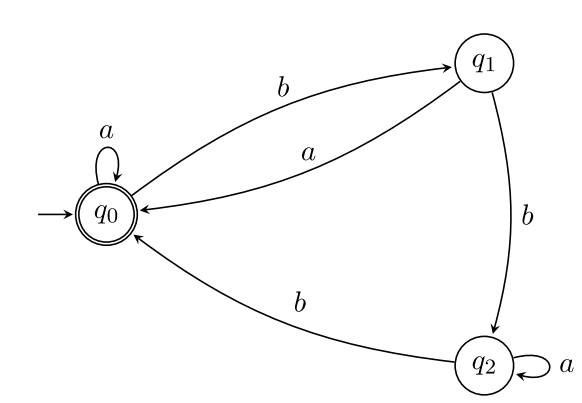
\includegraphics[width=0.7\textwidth]{pics/Blatt11_2.png}
 
\begin{lösung}
	\textbf{Lemma von Arden:}
	Seien $A,B\subseteq\Sigma^\ast$ und $\varepsilon\not\in A$.
	Dann hat
	\begin{align}\label{eqLemmaArden}\tag{Arden}
		X=A\cdot X\cup B
	\end{align}
	die eindeutige Lösung $X=A^\ast\cdot B$.\nl
	Wir erzeugen nun für jeden Zustand $q\in Q$ eine Gleichung.
	\begin{align}\label{eq2_1}
		X_0&=\lbrace a\rbrace\cdot X_0\cup\lbrace b\rbrace\cdot X_1\cup\lbrace\varepsilon\rbrace\\\label{eq2_2}
		X_1&=\lbrace a\rbrace\cdot X_0\cup\lbrace b\rbrace\cdot X_2\\
		X_2&=\lbrace a\rbrace\cdot X_2\cup\lbrace b\rbrace\cdot X_0\label{eq2_3}
	\end{align}
	Notizen:
	\begin{itemize}
		\item Bei Endzuständen muss $\cup\lbrace\varepsilon\rbrace$ ergänzt werden.
		\item Man schaut sich alle ausgehenden Transitionen an.
	\end{itemize}
	Wende nun Lemma von Arden auf \eqref{eq2_3} an:
	\begin{align}\label{eq2_4}
		X_2&=\lbrace a\rbrace^\ast\cdot\lbrace b\rbrace\cdot X_0 &\text{Lemma auf \eqref{eq2_3}}\\\nonumber
		X_1&=\lbrace a\rbrace\cdot X_0\cup\lbrace b\rbrace\cdot\lbrace a\rbrace^\ast\cdot\lbrace b\rbrace\cdot X_0 &\text{Einsetzen von \eqref{eq2_4} in \eqref{eq2_2}}\\
		&=\Big(\lbrace a\rbrace\cup\lbrace b\rbrace\cdot\lbrace a\rbrace^\ast\cdot\lbrace b\rbrace\Big)\cdot X_0\label{eq2_5}\\
		X_0&=\lbrace a\rbrace\cdot X_0\cup\lbrace b\rbrace\Big(\lbrace a\rbrace\cup\lbrace b\rbrace\cdot\lbrace a\rbrace^\ast\cdot\lbrace b\rbrace\Big)\cdot X_0\cup\lbrace\varepsilon\rbrace &\text{Einsetzen von \eqref{eq2_5} in \eqref{eq2_1}}\nonumber\\
		\overset{\text{Distr}}&{=}
		\Big(\lbrace a\rbrace\cup\lbrace b\rbrace\cdot\big(\lbrace a\rbrace\cup\lbrace b\rbrace\cdot\lbrace a\rbrace^\ast\cdot\lbrace b\rbrace\big)\Big)\cdot X_0\cup\lbrace\varepsilon\rbrace\label{eq2_6}\\
		X_0&=\Big(\lbrace a\rbrace\cup\lbrace b\rbrace\cdot\big(\lbrace a\rbrace\cup\lbrace b\rbrace\cdot\lbrace a\rbrace^\ast\cdot\lbrace b\rbrace\big)\Big)^\ast\cdot\lbrace\varepsilon\rbrace &\text{Lemma auf \eqref{eq2_6}}\nonumber\\
		&=L\Big(\big(a+b\cdot(a+ba^\ast b)\big)^\ast\Big)\nonumber\\
		&=L\Big(\big(a+ba+bba^\ast b\big)^\ast\Big)\nonumber
	\end{align}
\end{lösung} 

\subsection{Aufgabe 3}
Sei $\Sigma=\lbrace a,b,c\rbrace$.
 Geben Sie für jede der folgenden Sprachen $L_i$ einen regulären Ausdruck $r_i$ mit $L_i=L(r)$ an.
Erklären Sie die Wahl Ihrer regulären Ausdrücke $r_i$.

\begin{enumerate}[label=\alph*)]
	\item $L_1=\big\lbrace w\in\Sigma^\ast:w\text{ beginnt mit $a$ mit $|w|_b$ ist gerade}\big\rbrace$
	\item $L_2=\big\lbrace w\in\Sigma^\ast:\nexists u,v\in\Sigma^\ast:w=uaav\big\rbrace$
\end{enumerate}

\begin{lösung}
	Idee: 
	\begin{enumerate}
		\item Konstruiere NEA $\A_i$ mit $L(\A_i)=L_i$.
		\item Ermittle den regulären Ausdruck $r_i$ von $\A_i$ wie in Aufgabe 2.
	\end{enumerate}		

	\underline{Zeige a):}
	
	\usetikzlibrary{positioning,automata}
\begin{tikzpicture}[shorten >=1pt,node distance=2.7cm,on grid]
  \node[state,initial]   	(q_0)                		{$q_0$};
  \node[state, accepting] 	(q_1) [above right=of q_0] 	{$q_1$};
  \node[state] 	(q_2) [below=of q_1] 		{$q_2$};
  \path[->] (q_0) edge [bend left=0] node [above] {a} (q_1)
            (q_1) edge [loop right] node [above] {a,c} ()
            	  edge [bend left=30] node [left] {b} (q_2)
            (q_2) edge [loop right] node [right] {a,c} ()
                  edge [bend left=30] node [right] {b} (q_1)
       ;
\end{tikzpicture}

	$q_1\hat{=}$ "gerade Anzahl von b's gelesen"\\
	$q_2\hat{=}$ "ungerade Anzahl von b's gelesen"
	
	\begin{align}
		X_0&=\lbrace a\rbrace\cdot X_1\\
		X_1&=\lbrace a,c\rbrace\cdot X_1\cup\lbrace b\rbrace\cdot X_2\cup\lbrace\varepsilon\rbrace\\
		X_2&=\lbrace a,c\rbrace\cdot X_2\cup\lbrace b\rbrace\cdot X_1
	\end{align}
	
	Mit dem Lemma von Arden erhalten wir (anwenden auf letzte Gleichung):
	\begin{align*}
		X_2&=\lbrace a,c\rbrace^\ast\cdot\lbrace b\rbrace\cdot X_1\\
		X_1&=\lbrace a,c\rbrace\cdot X_1\cup\lbrace b\rbrace\cdot\lbrace a,c\rbrace^\ast\cdot\lbrace b\rbrace\cdot X_1\cup\lbrace\varepsilon\rbrace\\
		&=\Big(\lbrace a,c\rbrace\cup\lbrace b\rbrace\cdot\lbrace a,c\rbrace^\ast\cdot\lbrace b\rbrace\Big)\cdot X_1 \cup\lbrace\varepsilon\rbrace\\
		X_1&=\Big(\lbrace a,c\rbrace\cup\lbrace b\rbrace\cdot\lbrace a,c\rbrace^\ast\cdot\lbrace b\rbrace\Big)^\ast\cdot\lbrace\varepsilon\rbrace\\
		X_0&=\lbrace a\rbrace\cdot\Big(\lbrace a,c\rbrace\cup\lbrace b\rbrace\cdot\lbrace a,c\rbrace^\ast\cdot\lbrace b\rbrace\Big)^\ast\\
		&=L\Big(a\cdot\big((a+c)+b(a+c)^\ast b\big)^\ast\Big)=:r_i
	\end{align*}		
	
	\underline{Zeige b):}
	Sprache umschreiben:
	\begin{align*}
		L_2&=\big\lbrace w\in\Sigma^\ast:\nexists u,v\in\Sigma^\ast:w=uaav\big\rbrace\\
		&=\big\lbrace w\in\Sigma^\ast: w\text{ enthält keine zwei aufeinanderfolgenden $a$'s}\big\rbrace
	\end{align*}
	
	\begin{tikzpicture}[shorten >=1pt,node distance=2.7cm,on grid]
  \node[state,initial, accepting](q_0)           		{$q_0$};
  \node[state, accepting] 	(q_1) [right=of q_0] 	{$q_1$};
  \path[->] (q_0) edge [loop above] node [above] {b,c} ()
  				  edge [bend left=30] node [above] {a} (q_1)
            (q_1) edge [bend left=30] node [below] {b,c} (q_0)
       ;
	\end{tikzpicture}

	\begin{align*}
		r_1=\big(b+c+a\cdot(b+c)\big)^\ast\cdot(a+\varepsilon)
	\end{align*}
	
	
\end{lösung}


% This work is licensed under the Creative Commons
% Attribution-NonCommercial-ShareAlike 4.0 International License. To view a copy
% of this license, visit http://creativecommons.org/licenses/by-nc-sa/4.0/ or
% send a letter to Creative Commons, PO Box 1866, Mountain View, CA 94042, USA.

\section{Aufgabenblatt 12}
\subsection*{Aufgabe $\ast$)}
Die dritte Bedingung in $L$ sagt, dass die Wörter in $L$ nicht mit $a$ beginnen dürfen.
Kurz geschrieben (Achtung, keine offizielle Notation!)
\begin{align*}
	L=\Big\lbrace w=u_1 babc u_2,w=u_3 ccc u_4,w\neq a u_5:u_1,\ldots,u_5\in\Sigma^\ast\Big\rbrace
\end{align*}
Somit erhält man den Regulären Ausdruck 
\begin{align*}
	r=(b+c)^\ast\cdot(a+b+c)^\ast\cdot(b\cdot a\cdot b\cdot c+c\cdot c\cdot c)\cdot(a+b+c)^\ast
\end{align*}

\subsection*{Aufgabe $\ast\ast$)}
\begin{enumerate}[label=(\alph*)]
	\item $\begin{aligned}
		L(r_1)=\Big\lbrace b^m a^n:m\in\N_{\geq0},n\in\lbrace0,1\rbrace\Big\rbrace
	\end{aligned}$
	\item $\begin{aligned}
		L(r_1)=\Big\lbrace b^m a^n:m\in\N_{\geq0},n\in\lbrace0,1\rbrace\Big\rbrace
	\end{aligned}$
	\item $\begin{aligned}
		L(r_1)=\Big\lbrace b^m a^n:m\in\N_{\geq0},n\in\lbrace0,1\rbrace\Big\rbrace
	\end{aligned}$
\end{enumerate}

\subsection{Aufgabe 1}

\begin{lösung}
	\underline{Zeige a):}
	
	\underline{Zeige b):}
	
	
	\underline{Zeige c):}
	
	
	\underline{Zeige e):}
		
	\underline{Zeige f):}
	
\end{lösung}

\subsection{Aufgabe 2}

\begin{lösung}
	
\end{lösung} 

\subsection{Aufgabe 3}
Betrachte die Grammatik
\begin{align*}
	G_0&=\Big(\lbrace S,T,U,V,R\rbrace,\lbrace a,b\rbrace,P_0,S\Big)\\
	P_0&=\left\lbrace
		\begin{array}{c}
			 S\to\varepsilon,S\to aSb,S\to T,S\to R,\\
			 T\to bbT, T\to U\\
			 U\to aa U,U\to bbT\\
			 V\to bSa\\
			 R\to\varepsilon\\
			 R\to bSa
		\end{array}\right\rbrace		
\end{align*}
	
\subsubsection{Aufgabe 3 a)}
Geben Sie zu $G_0$ alle nicht-terminierenden Symbole und nicht-erreichbaren Symbole an und geben Sie eine zu $G_0$ äquivalente reduzierte Grammatik $G_1$ an.

\begin{lösung}
	%TODO
\end{lösung}

\subsubsection{Aufgabe 3 b)}
Konstruieren Sie eine Grammatik $G_2$ mit $L(G_2)=L(G_1)\setminus\lbrace\varepsilon\rbrace$, die keine Regeln der Form $A\to\varepsilon$ für $A\in N$ enthält.

\begin{lösung}
	%TODO
\end{lösung}

\subsubsection{Aufgabe 3 c)}
Geben Sie ein zu $G_1$ äquivalente $\varepsilon$-freie Grammatik $G_3$ an.
Erweitern Sie dazu, wenn nötig, die Grammatik $G_2$ um ein neues Startsymbol $S_3$ und entsprechende Regeln.

\begin{lösung}
	%TODO
\end{lösung}

\subsubsection{Aufgabe 3 d)}
Geben Sie eine zu $G_3$ äquivalente Grammatik $G_4$ an, die keine Produktionen der Form $A\to B$ mit Nichtterminalsymbolen $A,B$ enthält.

\begin{lösung}
	%TODO
\end{lösung}

\subsubsection{Aufgabe 3 e)}
Geben Sie eine zu $G_4$ äquivalente Grammatik $G_5$ in Chomsky-Normalform an.

\begin{lösung}
	%TODO
\end{lösung}
\breakCIbuild


	\listoffigures 
	%\listoftables
	%\bibliography{literatur}
\end{document}
